% Options for packages loaded elsewhere
\PassOptionsToPackage{unicode}{hyperref}
\PassOptionsToPackage{hyphens}{url}
%
\documentclass[
  a4paper,
]{scrbook}

\usepackage{amsmath,amssymb}
\usepackage{iftex}
\ifPDFTeX
  \usepackage[T1]{fontenc}
  \usepackage[utf8]{inputenc}
  \usepackage{textcomp} % provide euro and other symbols
\else % if luatex or xetex
  \usepackage{unicode-math}
  \defaultfontfeatures{Scale=MatchLowercase}
  \defaultfontfeatures[\rmfamily]{Ligatures=TeX,Scale=1}
\fi
\usepackage{lmodern}
\ifPDFTeX\else  
    % xetex/luatex font selection
  \setmainfont[]{Latin Modern Roman}
  \setsansfont[]{Latin Modern Roman}
\fi
% Use upquote if available, for straight quotes in verbatim environments
\IfFileExists{upquote.sty}{\usepackage{upquote}}{}
\IfFileExists{microtype.sty}{% use microtype if available
  \usepackage[]{microtype}
  \UseMicrotypeSet[protrusion]{basicmath} % disable protrusion for tt fonts
}{}
\makeatletter
\@ifundefined{KOMAClassName}{% if non-KOMA class
  \IfFileExists{parskip.sty}{%
    \usepackage{parskip}
  }{% else
    \setlength{\parindent}{0pt}
    \setlength{\parskip}{6pt plus 2pt minus 1pt}}
}{% if KOMA class
  \KOMAoptions{parskip=half}}
\makeatother
\usepackage{xcolor}
\setlength{\emergencystretch}{3em} % prevent overfull lines
\setcounter{secnumdepth}{5}
% Make \paragraph and \subparagraph free-standing
\ifx\paragraph\undefined\else
  \let\oldparagraph\paragraph
  \renewcommand{\paragraph}[1]{\oldparagraph{#1}\mbox{}}
\fi
\ifx\subparagraph\undefined\else
  \let\oldsubparagraph\subparagraph
  \renewcommand{\subparagraph}[1]{\oldsubparagraph{#1}\mbox{}}
\fi


\providecommand{\tightlist}{%
  \setlength{\itemsep}{0pt}\setlength{\parskip}{0pt}}\usepackage{longtable,booktabs,array}
\usepackage{calc} % for calculating minipage widths
% Correct order of tables after \paragraph or \subparagraph
\usepackage{etoolbox}
\makeatletter
\patchcmd\longtable{\par}{\if@noskipsec\mbox{}\fi\par}{}{}
\makeatother
% Allow footnotes in longtable head/foot
\IfFileExists{footnotehyper.sty}{\usepackage{footnotehyper}}{\usepackage{footnote}}
\makesavenoteenv{longtable}
\usepackage{graphicx}
\makeatletter
\def\maxwidth{\ifdim\Gin@nat@width>\linewidth\linewidth\else\Gin@nat@width\fi}
\def\maxheight{\ifdim\Gin@nat@height>\textheight\textheight\else\Gin@nat@height\fi}
\makeatother
% Scale images if necessary, so that they will not overflow the page
% margins by default, and it is still possible to overwrite the defaults
% using explicit options in \includegraphics[width, height, ...]{}
\setkeys{Gin}{width=\maxwidth,height=\maxheight,keepaspectratio}
% Set default figure placement to htbp
\makeatletter
\def\fps@figure{htbp}
\makeatother

\usepackage{booktabs}
\usepackage{longtable}
\usepackage{array}
\usepackage{multirow}
\usepackage{wrapfig}
\usepackage{float}
\usepackage{colortbl}
\usepackage{pdflscape}
\usepackage{tabu}
\usepackage{threeparttable}
\usepackage{threeparttablex}
\usepackage[normalem]{ulem}
\usepackage{makecell}
\usepackage{xcolor}
\usepackage{fancyhdr}
\usepackage{textcomp}
\usepackage{titling}
\usepackage{pdflscape}
\usepackage{geometry}
\setlength{\droptitle}{-2cm}
\preauthor{
  \begin{center}
  \Large
  \vspace{10mm}
  by
  \vspace{20mm}
}
\postauthor{
  \end{center}
  \vfill
}

\predate{
  \begin{center}
  A thesis 
  submitted in partial fulfilment of the \\
  requirements of the degree of \\
  Doctor of Philosophy in Physics\\               % Degree
  School of Physical and Chemical Sciences\\          % Department
  Te Herenga Waka - Victoria University of Wellington\\                       % University 
  \vspace{5mm}
}
\postdate{
  \\
  
\includegraphics[width=3in,height=1.5in]{figures/VUW-logo.png}\\
  \end{center}
  }

\renewcommand{\topfraction}{.8}
\renewcommand{\bottomfraction}{.7}
\renewcommand{\textfraction}{.15}
\renewcommand{\floatpagefraction}{.8}
\setcounter{topnumber}{3}
\setcounter{bottomnumber}{3}
\setcounter{totalnumber}{4}

\clubpenalty=9996
\widowpenalty=9999
\makeatletter
\makeatother
\makeatletter
\@ifpackageloaded{bookmark}{}{\usepackage{bookmark}}
\makeatother
\makeatletter
\@ifpackageloaded{caption}{}{\usepackage{caption}}
\AtBeginDocument{%
\ifdefined\contentsname
  \renewcommand*\contentsname{Table of contents}
\else
  \newcommand\contentsname{Table of contents}
\fi
\ifdefined\listfigurename
  \renewcommand*\listfigurename{List of Figures}
\else
  \newcommand\listfigurename{List of Figures}
\fi
\ifdefined\listtablename
  \renewcommand*\listtablename{List of Tables}
\else
  \newcommand\listtablename{List of Tables}
\fi
\ifdefined\figurename
  \renewcommand*\figurename{Figure}
\else
  \newcommand\figurename{Figure}
\fi
\ifdefined\tablename
  \renewcommand*\tablename{Table}
\else
  \newcommand\tablename{Table}
\fi
}
\@ifpackageloaded{float}{}{\usepackage{float}}
\floatstyle{ruled}
\@ifundefined{c@chapter}{\newfloat{codelisting}{h}{lop}}{\newfloat{codelisting}{h}{lop}[chapter]}
\floatname{codelisting}{Listing}
\newcommand*\listoflistings{\listof{codelisting}{List of Listings}}
\makeatother
\makeatletter
\@ifpackageloaded{caption}{}{\usepackage{caption}}
\@ifpackageloaded{subcaption}{}{\usepackage{subcaption}}
\makeatother
\makeatletter
\@ifpackageloaded{tcolorbox}{}{\usepackage[skins,breakable]{tcolorbox}}
\makeatother
\makeatletter
\@ifundefined{shadecolor}{\definecolor{shadecolor}{rgb}{.97, .97, .97}}
\makeatother
\makeatletter
\makeatother
\makeatletter
\makeatother
\ifLuaTeX
  \usepackage{selnolig}  % disable illegal ligatures
\fi
\usepackage[citestyle = ieee,urldate = iso8601]{biblatex}
\addbibresource{references.bib}
\IfFileExists{bookmark.sty}{\usepackage{bookmark}}{\usepackage{hyperref}}
\IfFileExists{xurl.sty}{\usepackage{xurl}}{} % add URL line breaks if available
\urlstyle{same} % disable monospaced font for URLs
\hypersetup{
  pdftitle={Developing an Insect Odorant Receptor Bioelectronic Nose for Vapour-Phase Detection},
  pdfauthor={Eddyn Oswald Perkins Treacher},
  hidelinks,
  pdfcreator={LaTeX via pandoc}}

\title{Developing an Insect Odorant Receptor Bioelectronic Nose for
Vapour-Phase Detection}
\author{Eddyn Oswald Perkins Treacher}
\date{Dec 2024}

\begin{document}
\frontmatter

\maketitle

\clearpage
\newpage
\thispagestyle{empty} % Hide header and footer on this page
\mbox{~}
\clearpage
\newpage

%----------------------------------------------
%   Abstract
%----------------------------------------------

\thispagestyle{plain}

\begin{flushleft}
% Manually add a section to the table of contents
\pagenumbering{roman}
\addcontentsline{toc}{chapter}{Abstract}
\huge\textbf{Abstract}
\end{flushleft}

\vspace*{\baselineskip}

The ability to detect volatile organic compounds in a highly sensitive and selective manner is desirable for applications as varied as diagnoses of illnesses at a remote clinic, monitoring of air in an industrial setting, or identification of invasive organisms at a biosecurity checkpoint. Historically, animal noses have been used for such tasks, as their combined sensitivity and selectivity are superior to traditional artificial sensors. However, training and deploying animals in such situations is both time and cost intensive. In recent years, an improved understanding of \textit{in vivo} biological sensing has driven efforts to mimic these highly efficient processes in an artificial sensor format. \\[5pt] To this end, a "bioelectronic nose" was developed. This sensor uses an artificial transducer to amplify responses of an insect odorant receptor protein to specific volatile compounds. Thin-film transistors were used as the amplifier element, given their low cost, small size and extreme sensitivity. Various thin-film morphologies were compared, and their suitability for bioelectronic nose development assessed. Transducers made using a novel steam-assisted thin-film deposition technique were found to have highly consistent device-to-device electrical properties relative to other films. Films made using this process typically showed more surface contamination than other morphologies, but their high sensitivity was confirmed with a non-specific sensing series in an aqueous environment. \\[5pt] One of the major challenges encountered in this thesis was variability in the quality of sensor functionalisation. Raman spectroscopy and fluorescence microscopy confirmed an existing non-covalent attachment method could successfully immobilise nanodiscs onto the transistor channel region. However, various sensors functionalised using the same procedure often exhibited no sensing activity. Extensive electrical characterisation indicated the presence of an unidentified contamination layer which prevented electrical interaction between the insect odorant receptors and the transducer thin-film. It was shown that this layer was unlikely to be directly associated with the thin-film morphology used for the transducer. \\[5pt] Subsequently, an alternative biotin-based non-covalent method was used for functionalisation of the proteins, which eliminated several possible sources of contamination. This alternative biotin-based method was used to demonstrate successful aqueous sensing of femtomolar concentrations of methyl salicylate by an iOR10a-functionalised device. When tested in a custom-built vapour delivery system, a similar bioelectronic sensor was shown to be highly sensitive to the target vapour. However, consistent reproduction of the biotin-based method was challenging due to the harsh cleaning method involved. It was therefore difficult to determine conclusively whether the vapour-phase sensor responses were selective. By finding new, systematic approaches to address the barriers to sensor success carefully identified in this work, there are promising signs that a highly reliable vapour-phase bioelectronic nose can be produced.

%\fancyhf{} %clear all headers and footers fields
%\thispagestyle{fancy} % Change header and footer on this page
%\renewcommand{\headrulewidth}{0pt}
%\fancyhead[L]{\textit{Abstract}} % Set header content
%\fancyfoot[L]{\thepage} %prints the page number on the right side of the header

\clearpage
\newpage
\thispagestyle{empty} % Hide header and footer on this page
\mbox{~}
\clearpage
\newpage


%----------------------------------------------
%   Acknowledgement
%----------------------------------------------

\thispagestyle{plain}

\begin{flushleft}
% Manually add a section to the table of contents
\addcontentsline{toc}{chapter}{Acknowledgements}
\huge\textbf{Acknowledgements}
\end{flushleft}

\vspace*{\baselineskip}

I would first like to acknowledge the lands of my ancestors, and the lands of the sovereign first peoples to which my ancestors travelled. We each come from the land, live off the land and return to the land.\\[5pt]
\textit{Noon of Essex to Warrang, on the Friends, Autumn 1811} \\[5pt]
\textit{Cave of Cambridgeshire to Warrang, on the Royal Charlotte, Autumn 1825} \\[5pt]
\textit{Boyce of Suffolk to Warrang, 1832} \\[5pt] 
\textit{Charlton of Northumberland to Warrang, on the Clyde, Spring 1834} \\[5pt]
\textit{Prouse of Devonshire to Pito-one, on the Duke of Roxburgh, Summer 1840} \\[5pt]
\textit{Ebden of Devonshire to Pito-one, on the Tyne, Winter 1841} \\[5pt]
\textit{Collis of Hampshire to Pito-one, on the Birman, Autumn 1842} \\[5pt]
\textit{Swann of Loch Garman to Te Whanganui-a-Tara, 1844} \\[5pt] 
\textit{Blythe of Berkshire to Whakatū, circa 1846} \\[5pt]
\textit{Innes of Berkshire to Naarm, on the Sacramento, Autumn 1853} \\[5pt]
\textit{Sheppard of Gloucestershire to Naarm, 1853} \\[5pt] 
\textit{Bruce of London to Naarm, on the Omega, Autumn 1855} \\[5pt]
\textit{Quennell of Surrey to Warrang, on the Asiatic, Winter 1855} \\[5pt]
\textit{Barr of Glasgow to Kōpūtai, on the Sir Edward Paget, Winter 1856} \\[5pt] 
\textit{Perkins of London to Te Whanganui-a-Tara, on the Matoaka, Spring 1859} \\[5pt]
\textit{McKee of Antrim to Tāmaki Makaurau, on the Indian Empire, Spring 1862} \\[5pt]
\textit{Sandilands of Peeblesshire to Ōtepoti, circa 1864} \\[5pt] 
\textit{Treacher of Berkshire to Te Whanganui-a-Tara, on the Wild Duck, Summer 1865} \\[5pt]
\textit{McTaggart of Argyllshire to Kōpūtai, on the Edward P. Bouverie, Autumn 1869} \\[5pt] 
\textit{Chapman of Kent to Whakatū, on the Adamant, Winter 1874} \\[5pt]
\textit{Cheel of London to Whakatū, on the Queen Bee, Winter 1877} \\[5pt]  
\textit{Hutchison of Aberdeen to Tarntanya, before 1882.} \\[5pt] 
I chose to start my doctoral studies just a few months into a global pandemic. Completing a challenging project with a worldwide crisis in the background might have been impossible without the supervision of AProf. Natalie Plank. Her ability to adapt to and overcome any problem has taught me that there is no situation which is truly unmanageable. I am deeply grateful for her leadership throughout a time of particular chaos. \newpage
\fancyhf{} %clear all headers and footers fields
\thispagestyle{fancy} % Change header and footer on this page
\renewcommand{\headrulewidth}{0pt}
\fancyhead[L]{\textit{Acknowledgements}} % Set header content
\fancyfoot[L]{\thepage} %prints the page number on the left side of the header 
I started this project with minimal formal training in biological science, coming from a primarily physics and engineering background. \\[5pt] The immense support I received from Melissa Jordan and Colm Carraher from the Institute for Plant and Food Research (PFR) to complete this project meant that this was not an issue, and I thank them both immensely for this. \\[5pt] I would not have been able to begin this thesis without the financial backing and support I received from PFR and the Better Border Biosecurity (B3) programme. In particular, I am very grateful to Andrew Kralicek, formerly with PFR and now at Scentian Bio, and the ex-Director of B3, David Teulon, for helping to secure funding for my project. I would also like to thank the donor of the Ernest Marsden Scholarship in Physics for their significant financial support. \\[5pt] There are many incredibly supportive people who I worked alongside during my project. I would like to start off by thanking Rifat Ullah, whose mentoring and kindness encouraged me to pursue further study. His work on the initial design and setup of the vapour delivery system was invaluable to me throughout this project. I am also especially grateful to Alex Puglisi, for constructing the mechanical elements of the vapour delivery system and giving me extensive feedback on the system design. I would like to thank Peter Coard, for his advice and guidance when constructing the electrical elements of the vapour delivery system. I thank Selvan Murugathas, too, for his advice on constructing the insect odorant receptor sensors, as well as Damon Colbert and Valentina Lucarelli, who provided the insect odorant receptor nanodiscs used in this work. \\[5pt] Thank you to AProf. Ben Ruck, my supportive secondary supervisor, and to AProf. Franck Natali, for always asking about my thesis in the tearoom. Thank you to Gideon Gouws for his friendly encouragement and advice. For their substantial technical assistance and mentoring during this project, I thank Alan Rennie, Grant Franklin, Chris Lepper, Rashika Gunasekara, Pete Jebson and Sushila Pillai from VUW, Andrew Chan from PFR, AProf. Charles Unsworth from the University of Auckland, and Prof. Simon Brown and his nanomaterials group from the University of Canterbury. \\[5pt] I was lucky enough to start my doctoral program just as a group of supportive and talented senior students were finishing, and finished just as a group of enthusiastic and talented new doctoral students were starting. A special thanks to Jenna Nyugen, Erica Happe and Erica Cassie for teaching me the fabrication processes and characterisation procedures that made this thesis happen; and a special thanks to Marissa Dierkes, Danica Fontein, Sangar Begzaad and Alireza Zare, for their incredible support throughout the thesis writing process. I am also thankful for the assistance of the cleanroom group interns over the course of my PhD, including Liam, Hayden and Lotte. I would further like to thank everyone else I shared an office with and worked alongside, including Jackson, Will, Roshni, Ali, Sam, Kira, Catherine, Martin, Janani, Ted, Kiri and Joe. \\[5pt] A massive thank you to Openstar Technologies. It has been an honour to work on a cutting-edge plasma physics project right here in Te Whanganui-a-Tara. A particularly big thank you to Ratu, Darren and Thomas for having me as part of the plasma physics team. Thank you also to the other Openstar interns, in particular the other plasma physics interns, Valentina, Benjy and Chris. I wish you success in all your dipole-confined plasma related endeavours. \\[5pt] I want to thank Shodokan Aikido New Zealand for their support throughout this thesis, in particular for the once-in-a-lifetime opportunity to travel to Osaka to be graded for first-dan by Nariyama Shihan. Thanks for all the training and support, Ian. \\[5pt] Thank you to all the friends and whānau, old and new, who have supported me over these wild past few years. You know who you are. \\[5pt] Thank you to my brother, Keeson, and to my parents, Hilary and Phillip. Your support means everything to me, and I would not be where I am today without you. Our Friday lunchtime cafe visits kept me motivated and inspired throughout the doctoral program. Thank you, thank you, thank you for your love, your compassion, and for being there for me. \\[5pt] Finally, thank you Nina. Your incredible love has kept me going through the most difficult and most wonderful times over the last four years. You are the light of my life, and I am so happy to have taken on this challenge with you by my side. \\[5pt] Arohanui and peace to you all, Eddyn (Ned)

\fancyhf{} %clear all headers and footers fields
\thispagestyle{fancy} % Change header and footer on this page
\renewcommand{\headrulewidth}{0pt}
\fancyhead[R]{\textit{Acknowledgements}} % Set header content
\fancyfoot[R]{\thepage} %prints the page number on the right side of the header

\clearpage
\newpage
\thispagestyle{empty} % Hide header and footer on this page
\mbox{~}
\clearpage
\newpage

\pagestyle{headings}

\ifdefined\Shaded\renewenvironment{Shaded}{\begin{tcolorbox}[sharp corners, frame hidden, breakable, borderline west={3pt}{0pt}{shadecolor}, enhanced, boxrule=0pt, interior hidden]}{\end{tcolorbox}}\fi

\renewcommand*\contentsname{Table of Contents}
{
\setcounter{tocdepth}{2}
\addcontentsline{toc}{chapter}{Table of Contents}
\tableofcontents
}
\listoffigures
\addcontentsline{toc}{chapter}{List of Figures}
\listoftables
\addcontentsline{toc}{chapter}{List of Tables}

\clearpage
\newpage
\thispagestyle{empty} % Hide header and footer on this page
\mbox{~}
\clearpage
\newpage

%----------------------------------------------
%   List of Abbreviations
%----------------------------------------------

\thispagestyle{plain}

\begin{flushleft}
% Manually add a section to the table of contents
\addcontentsline{toc}{chapter}{List of Abbreviations}
\huge\textbf{List of Abbreviations}
\end{flushleft}

\vspace*{\baselineskip}

\begin{table}[H]
  \begin{tabular}{@{}p{0.25\textwidth} p{0.75\textwidth}@{}}  % Adjust the width as needed
    2D  & 2-Dimensional  \\[5pt]
    Ab  & Antibody  \\[5pt]
    AB  & Amyl Butyrate  \\[5pt]
    AB-NTA  & N$\alpha$,N$\alpha$-Bis(carboxymethyl)-\textit{L}-lysine hydrate  \\[5pt]
    AFM  & Atomic Force Microscope/Microscopy  \\[5pt]
    AH  & Absolute Humidity  \\[5pt]
    Avi-tag  & Avidin-tag  \\[5pt]
    BMIM  & 1-butyl-3-methylimidazolium bis(trifluoromethylsulfonyl)imide  \\[5pt]
    BWF  & Breit-Wigner-Fano  \\[5pt]
    CAD  & Computer Aided Design \\[5pt]
    CNT  & Carbon Nanotube  \\[5pt]
    CVD  & Chemical Vapour Deposition  \\[5pt]
    Cy3  & Cyanine 3  \\[5pt]
    DAN  & 1,5-diaminonaphthalene  \\[5pt]
    DAQ  & Data Acquisition Input/Output Module  \\[5pt]
    DCB  & 1,2-dichlorobenzene  \\[5pt]
    DI  & Deionised  \\[5pt]
    DMF  & Dimethylformamide   \\[5pt]
    DMSO  & Dimethylsulfoxide   \\[5pt]
    DMT-MM   & 4-(4,6-dimethoxy-1,3,5-triazin-2-yl)-4 methylmorpholinium chloride \\[5pt]
    DMMP  & Dimethyl Methylphosphonate  \\[5pt]
    DNA  & Deoxyribonucleic Acid  \\[5pt]
    E2Hex  & \textit{trans}-2-hexan-1-al  \\[5pt]
    EB  & Ethyl Butyrate  \\[5pt]
    EDC  & 1-Ethyl-3-(3-dimethylaminopropyl)carbodiimide  \\[5pt]
    EDL  & Electric Double Layer  \\[5pt]
    EIS  & Electrochemical Impedance Spectroscopy  \\[5pt]
    EtHex  & Ethyl Hexanoate  \\[5pt]
  \end{tabular}
\end{table}

\newpage
\fancyhf{} %clear all headers and footers fields
\thispagestyle{fancy} % Change header and footer on this page
\renewcommand{\headrulewidth}{0pt}
\fancyhead[L]{\textit{List of Abbreviations}} % Set header content
\fancyfoot[L]{\thepage} %prints the page number on the right side of the header
\begin{table}[H]
  \begin{tabular}{@{}p{0.25\textwidth} p{0.75\textwidth}@{}}  % Adjust the width as needed
    EtOH  & Ethanol  \\[5pt]
    FET  & Field-Effect Transistor  \\[5pt]
    FITC  & Fluorescein isothiocyanate  \\[5pt]
    GA  & Glutaraldehyde  \\[5pt]
    GFET  & Graphene Field-Effect Transistor  \\[5pt]
    GFP  & Green Fluorescent Protein  \\[5pt]
    GPCR  & G-protein Coupled Receptor  \\[5pt]
    HEK  & Human Embryonic Kidney  \\[5pt]
    His-tag  & Histidine-tag  \\[5pt]
    hOR  & Human Odorant Receptor  \\[5pt]
    HPLC  & High-performance Liquid Chromatography   \\[5pt]
    iOR  & Insect Odorant Receptor  \\[5pt]
    IPA  & Isopropanol  \\[5pt]
    LOD  & Limit of Detection  \\[5pt]
    m-CNT  & Metallic Carbon Nanotube   \\[5pt]
    MeOH  & Methanol   \\[5pt]
    MeSal  & Methyl Salicylate   \\[5pt]
    MFC  & Mass Flow Controller   \\[5pt]
    mOR  & Mouse Odorant Receptor  \\[5pt]
    MOSFET  & Metal-Oxide-Semiconductor Field-Effect Transistor  \\[5pt]
    MSP  & Membrane Scaffold Protein  \\[5pt]
    MWCNT  & Multi-Walled Carbon Nanotube  \\[5pt]
    ND  & Nanodisc  \\[5pt]
    NHS  & N-Hydroxysuccinimide  \\[5pt]
    NHSS  & N-hydroxysulfosuccinimide   \\[5pt]
    NMR  & Nuclear Magnetic Resonance  \\[5pt]
    NSB  & Non-Specific Binding   \\[5pt]
    NTA  & Nitrilotriacetic Acid   \\[5pt]
    OBP  & Odorant Binding Protein  \\[5pt]
    OR  & Odorant Receptor  \\[5pt]
    ORCO  & Odorant Receptor Co-Receptor  \\[5pt]
    PBA  & 1-Pyrenebutyric Acid  \\[5pt]
  \end{tabular}
\end{table}

\newpage
\fancyhf{} %clear all headers and footers fields
\thispagestyle{fancy} % Change header and footer on this page
\renewcommand{\headrulewidth}{0pt}
\fancyhead[R]{\textit{List of Abbreviations}} % Set header content
\fancyfoot[R]{\thepage} %prints the page number on the right side of the header
\begin{table}[H]
  \begin{tabular}{@{}p{0.25\textwidth} p{0.75\textwidth}@{}}  % Adjust the width as needed
    PBASE  & 1-Pyrenebutanoic Acid N-hydroxysuccinimide Ester  \\[5pt]
    PBS  & Phosphate-Buffered Saline  \\[5pt]
    PCB  & Printed Circuit Board   \\[5pt]
    PDL & Poly-\textit{D}-lysine  \\[5pt]
    PDMS  & Polydimethylsiloxane   \\  [5pt]
    PEG  & Polyethylene Glycol  \\[5pt] 
    PID  & Photoionisation Detector  \\[5pt]
    P\&ID & Process \& Instrumentation Diagram  \\[5pt]
    PLL  & Poly-\textit{L}-lysine  \\[5pt]
    PPB  & Pyrene-PEG-Biotin  \\[5pt]
    PPF  & Pyrene-PEG-FITC  \\[5pt]
    PPN  & Pyrene-PEG-NTA  \\[5pt]
    PPR  & Pyrene-PEG-Rhodamine  \\[5pt]
    PTFE  & Polytetrafluoroethylene (Teflon™)  \\[5pt]
    PVC  & Polyvinyl chloride  \\[5pt]
    QCM  & Quartz Crystal Microbalance  \\[5pt]
    RH  & Relative Humidity  \\[5pt]
    RHI  & Relative Humidity and Temperature Indicator  \\[5pt] 
    RNA  & Ribonucleic Acid   \\[5pt]
    SAW  & Surface Acoustic Wave   \\[5pt]
    s-CNT  & Semiconducting Carbon Nanotube   \\[5pt]
    SEM  & Scanning Electron Microscope/Microscopy   \\[5pt]
    SMU  & Source Measure Unit   \\[5pt]
    SPR  & Surface Plasmon Resonance   \\[5pt]
    SWCNT  & Single-Walled Carbon Nanotube   \\[5pt]
    TFTFET  & Thin-Film Field-Effect Transistor  \\[5pt]
    TMAH  & Tetramethylammonium hydroxide  \\[5pt]
    TX  & Transfer Characteristics  \\[5pt]
    UV  & Ultraviolet  \\[5pt]
    VI  & Virtual Instrument  \\[5pt]
    VUAA1  & N-(4-Ethylphenyl)-2-{[4-ethyl-5-(pyridin-3-yl)-4H-1,2,4-triazol-3-yl]sulfanyl}acetamide  \\[5pt] 
  \end{tabular}
\end{table}

\clearpage
\newpage
\thispagestyle{empty} % Hide header and footer on this page
\mbox{~}
\clearpage
\newpage

% Adjust the top and bottom margins of float pages to center floats
\makeatletter
\setlength{\@fptop}{0pt plus 1fil}
\setlength{\@fpbot}{0pt plus 1fil}
\makeatother

\pagestyle{headings}
\mainmatter
\bookmarksetup{startatroot}

\hypertarget{introduction}{%
\chapter{Introduction}\label{introduction}}

\hypertarget{background}{%
\section{Background}\label{background}}

The ``bioelectronic nose'', an electronic transducer modified with
elements of the animal olfactory system, has the potential to allow
specific detection of airborne volatile compounds at concentrations as
low as parts per trillion
\autocite{Glatz2011,Kwon2015,Dung2018,Kim2022a}. An ideal transducer
platform is the thin-film transistor (TFT) which is particularly
portable, simple to use, small and robust
\autocite{Kauffman2008,Khan2020}. The thin films used in these
field-effect transistors (FETs) include carbon nanotube networks and
graphene, low-dimensional nanomaterials which are both highly sensitive
and biocompatible \autocite{Shkodra2021}. The implications of successful
development of such a portable and robust bioelectronic nose are
significant. Applications could be found in high-importance fields such
as biosecurity, medicine, environmental protection and food safety
\autocite{Dung2018,Arakawa2019,Yang2017,Son2017}. For example, it has
been demonstrated that it is possible to detect invasive brown
marmorated stinkbugs based on their volatile trace \autocite{Moser2020}.
A bioelectronic nose could potentially accomplish this biosecurity task
far more cheaply and efficiently than trained sniffer dogs
\autocite{Lee2010,Moon2020,Terutsuki2020}. There has been rapid progress
in the development of bioelectronic noses using carbon nanotube
field-effect transistors (CNT FETs) and graphene field-effect
transistors (GFETs) over the past 15-20 years
\autocite{Yoon2009,Lee2010,Yang2018}.

Insect odorant receptors (iORs) enable simple invertebrates, such as the
vinegar fruit fly \emph{Drosophila melanogaster}, to distinguish between
a huge number of specific volatile compounds
\autocite{Hallem2004,Smart2008,Wicher2008,Munch2016,Bohbot2020}. Within
the past five years, a variety of \emph{Drosophila melanogaster} iORs
have been successfully coupled with highly sensitive low-dimensional
thin-film transistors (TFTs) for specific detection of fruit-like odors
in an aqueous environment \autocite{Murugathas2019a,Murugathas2020}.
iORs have also been used for sensitive and selective volatile detection
in a lipid bilayer format, but not in a portable bioelectronic nose
format \autocite{Yamada2021}. In this thesis, my aim was to investigate
whether a bioelectronic nose capable of odorant detection in a
vapour-phase environment could be constructed by coupling iORs with
TFTs. Alongside practical applications, development of a vapour-phase
bioelectronic nose using iORs may give us a greater understanding of the
mechanisms underlying insect olfaction \autocite{Lee2010}. The
transduction mechanism of nanomaterial-based iOR sensors is still
unknown, and I hope to shed further light on the biological and
electronic processes underpinning this mechanism
\autocite{Murugathas2020,Khadka2019,Cheema2021}.

\hypertarget{thesis-outline}{%
\section{Thesis Outline}\label{thesis-outline}}

This thesis consists of nine chapters. The first three chapters,
including this one, are background chapters introducing the general
topics of this thesis. The fourth and fifth chapters are methods
chapters, while the next three chapters (sixth, seventh and eight)
describe the results obtained. The ninth chapter concludes the thesis
and discusses possible next steps for future research.

\textbf{Chapter 2} gives a broad description of carbon nanotube and
graphene field-effect transistors with a focus on their use in sensing
applications. The chapter begins by looking at the general structure and
properties of thin-film transistors, where key figures of merit such as
transconductance, on-off ratio, gate current and hysteresis are
described. Graphene field-effect transistors (GFETs) and carbon nanotube
network field-effect transistors (CNT FETs) are then discussed in
greater detail. These descriptions include the chemical composition of
each nanomaterial, their conduction behaviour and their unique sensor
properties when integrated into a field-effect transistor as a
thin-film.

\textbf{Chapter 3} investigates existing odorant receptor-coupled
thin-film field-effect transistors in the literature. First, the
biological structure of odorant receptors and membrane formats for their
protection \emph{in vitro} are discussed. Details are then provided
regarding the construction and operation of existing vertebrate odorant
receptor TFT biosensors. The structure and function of the insect
odorant receptor is then contrasted with the vertebrate odorant
receptor, and existing insect odorant receptor TFT biosensors in the
literature are discussed. The chapter finishes with a brief discussion
of non-specific binding and its role in hindering biosensor activity.

\textbf{Chapter 4} describes the fabrication of the CNT FET and GFET
transducers used in this thesis and the characterisation techniques used
to probe their behaviour. The chapter starts with an introduction to
photolithography for thin-film transistor device fabrication. Various
techniques are described for random deposition of carbon nanotube
networks to act as channels for these thin-film transistors.
Characterisation techniques described in this chapter include atomic
force microscopy (AFM), fluorescence microscopy, Raman spectroscopy and
electrical characterisation with various semiconductor device analysers.

\textbf{Chapter 5} presents the results obtained from the use of
characterisation techniques on the pristine GFETs and CNT FETs. Various
carbon nanotube (CNT) network morphologies are displayed and analysed.
The Raman spectra and electrical device parameters of these CNT network
morphologies are then discussed, along with electrical parameters from
graphene devices. The sensitivity of a dense CNT network morphology
device is then verified in the aqueous phase.

\textbf{Chapter 6} explores the non-covalent functionalisation of GFETs
and CNT FETs with various linker molecules for insect odorant receptor
attachment. The linker molecules tested were 1-pyrenebutanoic acid
N-hydroxysuccinimide ester (PBASE) and 1-pyrenebutyric acid (PBA) with
1-Ethyl-3-(3-dimethylaminopropyl)carbodiimide (EDC). Pyrene-NTA and
pyrene-biotin were also investigated as other possible linker molecules.
The quality of various functionalisation approaches was then explored
with various fluorescently-tagged linker molecules and biomolecules. In
this process, various potential obstacles to successful biosensor
functionalisation were identified.

\textbf{Chapter 7} maps out progress made towards the creation of an
insect odorant receptor functionalised TFT biosensor for use in a
vapour-phase environment. Two different approaches are described that
gave rise to working aqueous-phase biosensors. The first
functionalisation approach, which used PBASE in methanol, led to
irreproducible results when biosensing. Possible factors causing the
unreliability of this method were then investigated. A second approach
was then designed to avoid the malign influence of any identified
factors.

\textbf{Chapter 8} outlines the development of a vapour delivery system
for characterisation of the insect odorant receptor functionalised TFT
biosensors in a vapour-phase environment. The vapour delivery system was
upgraded from an existing system to include new mass flow controllers,
to have greater control of flow through the system, and off the shelf
vapour sensors, to collect vapour flow data that could be used for
comparison against biosensor activity. The chapter also describes the
design and construction of an electronic interface to monitor and
control the components of the vapour delivery system, and calibration of
the system.

\textbf{Chapter 9} details the use of the vapour delivery system for
testing the functionalised biosensors in the vapour phase. First, the
flow behaviour of volatile organic vapours through the system was
validated using onboard reference sensors. The response of a pristine
carbon nanotube device to two volatile compounds is then compared to the
response of carbon nanotube devices functionalised using the second
functionalisation approach discussed in the previous chapter.

\textbf{Chapter 10} summarises the conclusions drawn from this work, and
proposes various related studies which can be undertaken to continue the
work described in this thesis.

\bookmarksetup{startatroot}

\hypertarget{sec-thin-film-transistors}{%
\chapter{Carbon Nanotube and Graphene Field-Effect
Transistors}\label{sec-thin-film-transistors}}

\hypertarget{introduction-1}{%
\section{Introduction}\label{introduction-1}}

There are many transducer options available for creating a biosensor
platform, including electrochemical impedance spectroscopy (EIS), quartz
crystal microbalance (QCM), surface acoustic wave (SAW), surface plasmon
resonance (SPR) and fluorescence-based detectors. However, the small
size, low cost, high biological compatibility and fast response time of
field-effect transistors give them a distinct advantage over alternative
platforms \autocite{Khan2020,Shkodra2021,Hirata2021}. Field-effect
transistors (FETs), initially proposed in the 1930s, consist of two
conductive electrodes on either side of a semiconducting channel, the
``source'' and ``drain'' electrodes, alongside an isolated ``gate''
electrode which is typically perpendicular to the channel. An applied
electric field from the gate electrode capacitively controls channel
resistance, giving rise to the label ``field-effect''. By adjusting gate
voltage, the flow of charge carriers between source and drain can be
varied over several orders of magnitude. The ability of this simple
structure to obtain a large signal response from small changes in
channel behaviour means field-effect transistors can be used as
high-quality amplifiers for sensor applications
\autocite{Kauffman2008,Petti2016,Tran2016,Shkodra2021,Yao2021}.

Carbon nanotube network and graphene field-effect transistors (CNT FETs
and GFETs) are both examples of a class of field-effect transistors
called thin-film transistors (TFTs). Thin-film transistors were first
developed in 1962 \autocite{Weimer1962}, and are closely related to the
commonly-used metal oxide semiconductor field-effect transistor
(MOSFET). Unlike MOSFETs, thin-film transistors do not use the substrate
as the device channel. Instead, current passes through a semiconducting
film on the surface of the device; the films discussed here are graphene
and carbon nanotubes, two carbon-based low-dimension nanomaterials.
Since thin-film transistors do not require a conductive substrate, they
can be fabricated using light, flexible and stretchable substrates,
making them significantly more versatile than MOSFETs
\autocite{Kauffman2008,Cao2009,Petti2016,Shkodra2021}. Invisible
conductive thin-films such as metal oxides and carbon nanotube networks
can also be used to create transparent electronics \autocite{Cao2009}.
While the principle of modulating current with a gate electrode is
shared by the MOSFET and TFT, the underlying physics behind the
transistor behaviour differs between the two. The MOSFET is turned on by
the change in carrier behaviour when switching from a depletion to an
inversion mode, while this is not the case for a TFT
\autocite{Petti2016}. Details of graphene and carbon nanotube TFT
switching behaviours can be found in the subsequent sections.

\hypertarget{sec-general-FETs}{%
\section{Thin-Film Field-Effect Transistors}\label{sec-general-FETs}}

\hypertarget{sec-gating}{%
\subsection{Structure and Gating}\label{sec-gating}}

\begin{figure}

\begin{minipage}[t]{0.03\linewidth}

{\centering 

\raisebox{-\height}{


\includegraphics{figures/(a).png}

}

}

\end{minipage}%
%
\begin{minipage}[t]{0.01\linewidth}

{\centering 

~

}

\end{minipage}%
%
\begin{minipage}[t]{0.45\linewidth}

{\centering 

\raisebox{-\height}{

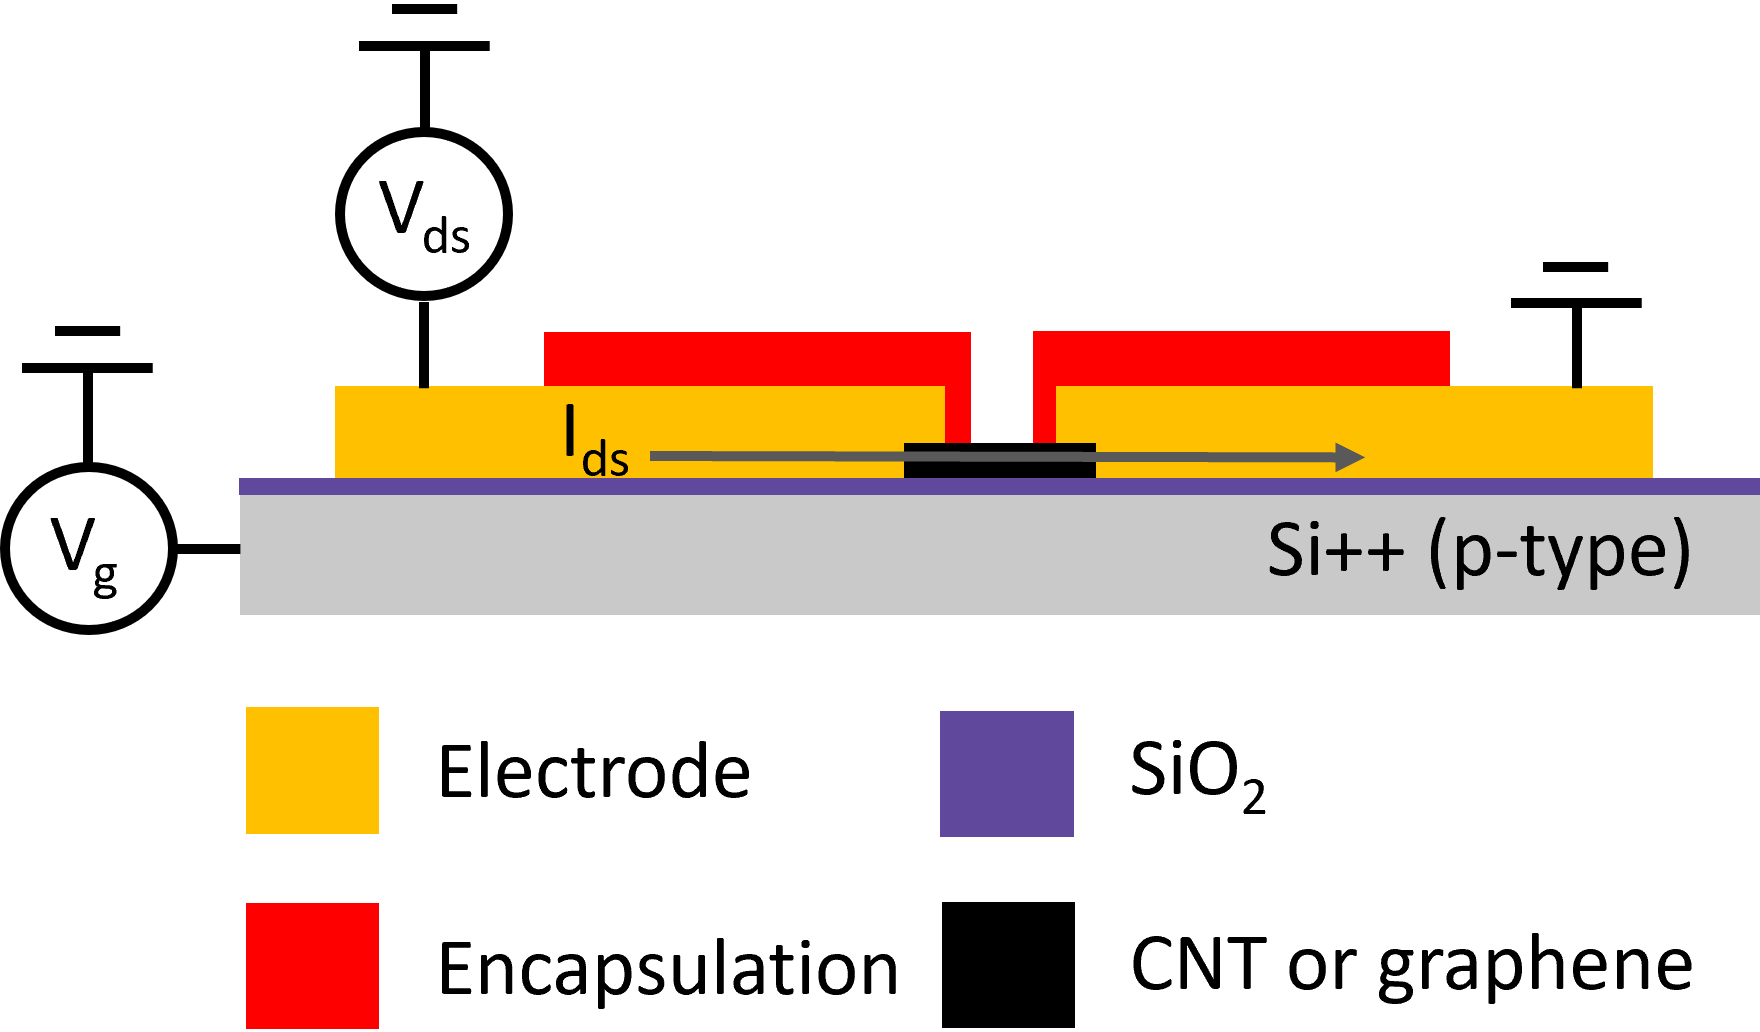
\includegraphics{figures/ch2/back-gate-schematic.png}

}

}

\end{minipage}%
%
\begin{minipage}[t]{0.01\linewidth}

{\centering 

~

}

\end{minipage}%
%
\begin{minipage}[t]{0.03\linewidth}

{\centering 

\raisebox{-\height}{


\includegraphics{figures/(b).png}

}

}

\end{minipage}%
%
\begin{minipage}[t]{0.01\linewidth}

{\centering 

~

}

\end{minipage}%
%
\begin{minipage}[t]{0.45\linewidth}

{\centering 

\raisebox{-\height}{

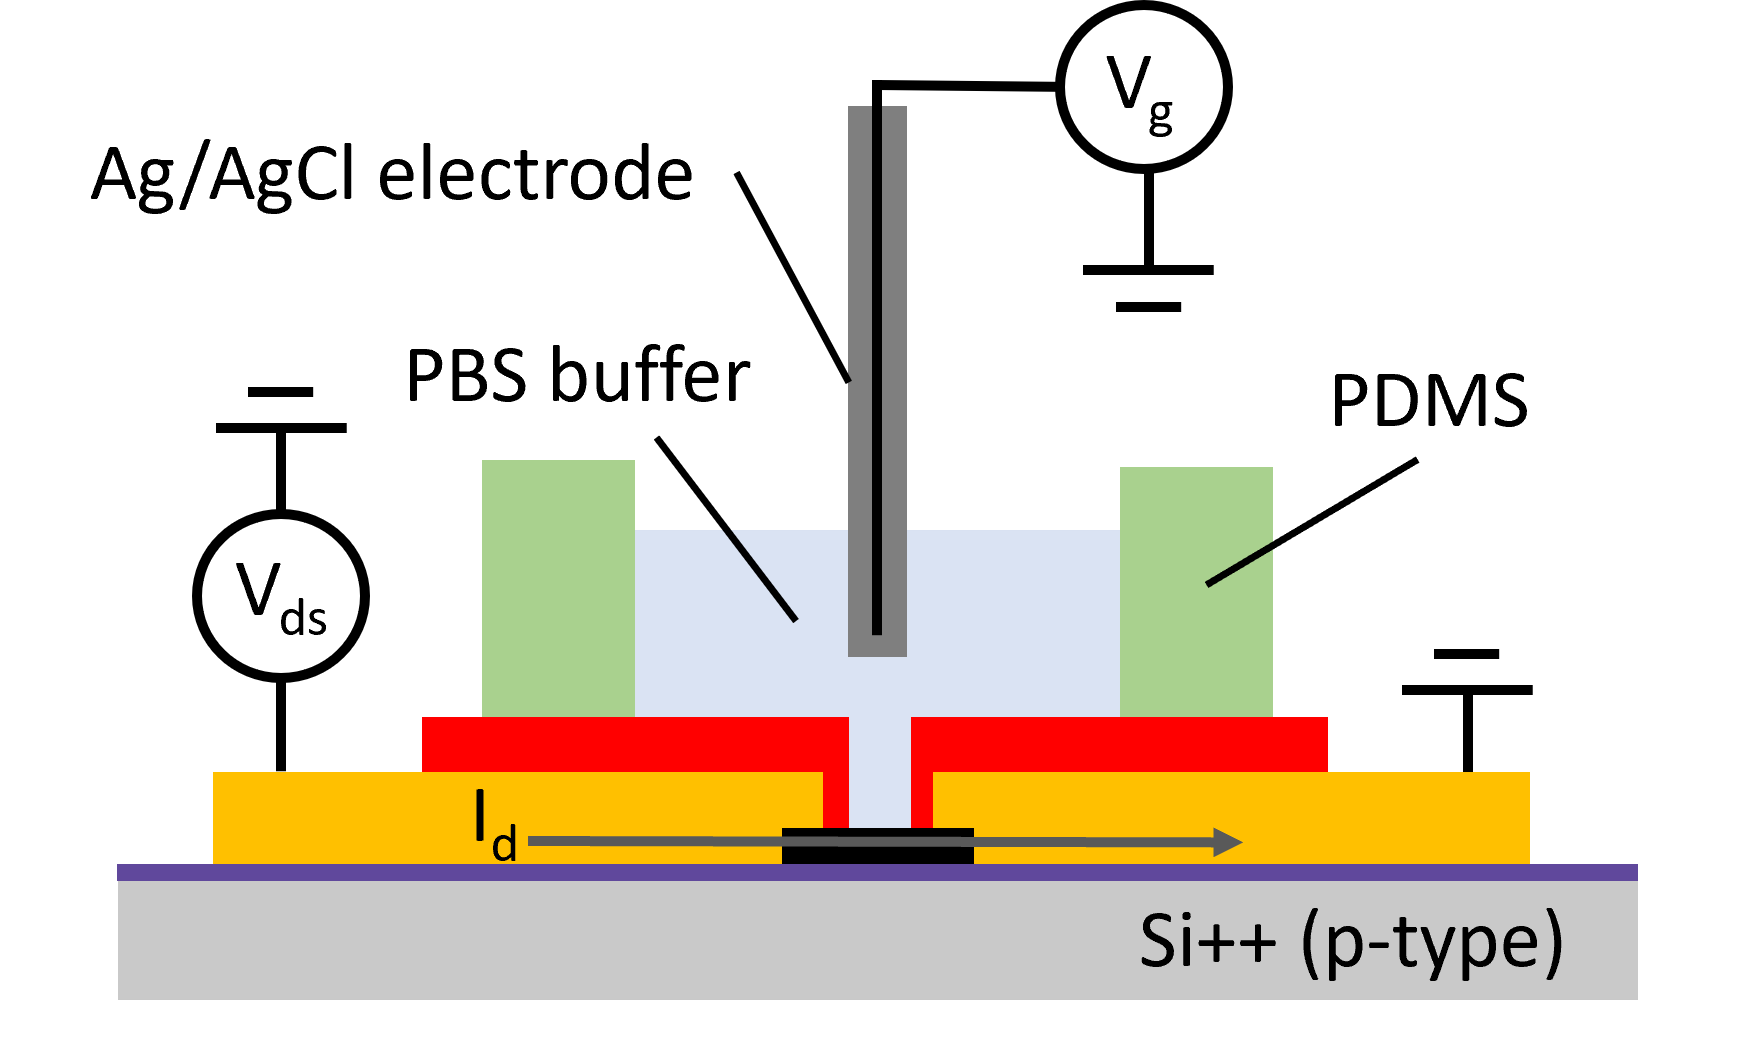
\includegraphics{figures/ch2/liquid-gate-schematic.png}

}

}

\end{minipage}%
%
\begin{minipage}[t]{0.01\linewidth}

{\centering 

~

}

\end{minipage}%

\caption[Schematics showing cross-sections of a thin-film
transistor.]{\label{fig-gating-schematics}Schematics (not to scale)
showing the side-view cross-section of a thin-film field-effect
transistor in both the (a) back-gated and (b) liquid-gated
configuration. Here, a graphene monolayer or a carbon nanotube network
is used as the transistor thin-film. The drain electrode is the gold
contact on the left side of each figure, while the source electrode is
the gold contact on the right.}

\end{figure}

Two basic configurations of the thin-film transistor are the back-gated
field-effect transistor and the liquid-gated (or electrolyte-gated)
transistor. The relatively simple back-gated configuration, shown in
Figure~\ref{fig-gating-schematics} (a), uses the degenerately doped Si
substrate as the gate. The channel is isolated from the gate with a thin
SiO\(_2\) layer. A liquid-gated device, shown in
Figure~\ref{fig-gating-schematics} (b), is used for sensitive
liquid-phase analyte detection. A submerged Ag/AgCl reference electrode
is generally used as a top-gate in this configuration. The channel is
isolated from the gate by the bulk of an electrolyte solution, which can
be restricted to the channel area using a hydrophobic
polydimethylsiloxane microchamber or ``PDMS well''. The electrolyte used
is typically the biofriendly phosphate-buffered saline (PBS), but other
aqueous salt solutions, polymers and ion-gels have also been used
\autocite{Avouris2007,Shkodra2021,Tran2016,Li2023}. Transistor operation
is controlled by a ``drain'' bias \(V_{ds}\), placed between the drain
and source electrodes, and a ``gate'' bias \(V_g\), placed between the
gate and source electrodes. Gate capacitance determines the influence of
\(V_g\) on drain-source current \(I_d\). In general, gate capacitance is
a series combination of geometric capacitance, \(C_{G}\), and the
quantum capacitance of the channel nanomaterial, \(C_{Q}\) (the change
in charge with respect to the electrochemical potential of a system)
\autocite{Avouris2007,Cao2009,Heller2009a,Tran2016,Miranda2016,Kireev2017,Li2023}.

\hypertarget{liquid-gating-and-debye-length}{%
\subsubsection*{Liquid-Gating and Debye
Length}\label{liquid-gating-and-debye-length}}
\addcontentsline{toc}{subsubsection}{Liquid-Gating and Debye Length}

Understanding the ionic behaviour of the gate electrolyte used in a
liquid-gated device setup gives insight into the gating and sensing
behaviour of the setup. When a voltage is applied at the liquid-gate,
the charged ions in solution move to form two electric double layers,
one at the interface between the electrolyte and gate electrode, and one
at the interface between electrolyte and semiconducting channel, as
shown in Figure~\ref{fig-Debye-length}. The gate capacitance is a series
combination of the capacitance of each EDL in series with quantum
capacitance \(C_{Q}\) \autocite{Heller2010,Kireev2017,Shkodra2021}. The
Gouy-Chapman-Stern model splits the EDL into two distinct regions, the
first being a compact layer of ions, the Stern layer, and the second
being a more diffuse layer, the Gouy-Chapman layer
\autocite{Tiwari2022}. The surface potential of the solid-electrolyte
interface exponentially decreases across the diffuse region of the
double-layer; the characteristic length of this potential screening is
known as Debye length, \(\lambda_D\). The typical electrolyte Debye
length is on a nanometer scale, therefore the bulk electrolyte acts as
an insulator, similar to the SiO\(_2\) dielectric in the back-gated
configuration. The Stern layer capacitance is inversely proportional to
the Debye length, and therefore decreased \(\lambda_D\) corresponds to
increased gate capacitance
\autocite{Heller2010,Ohno2015,Shkodra2021,Yao2021}.

\begin{figure}

{\centering 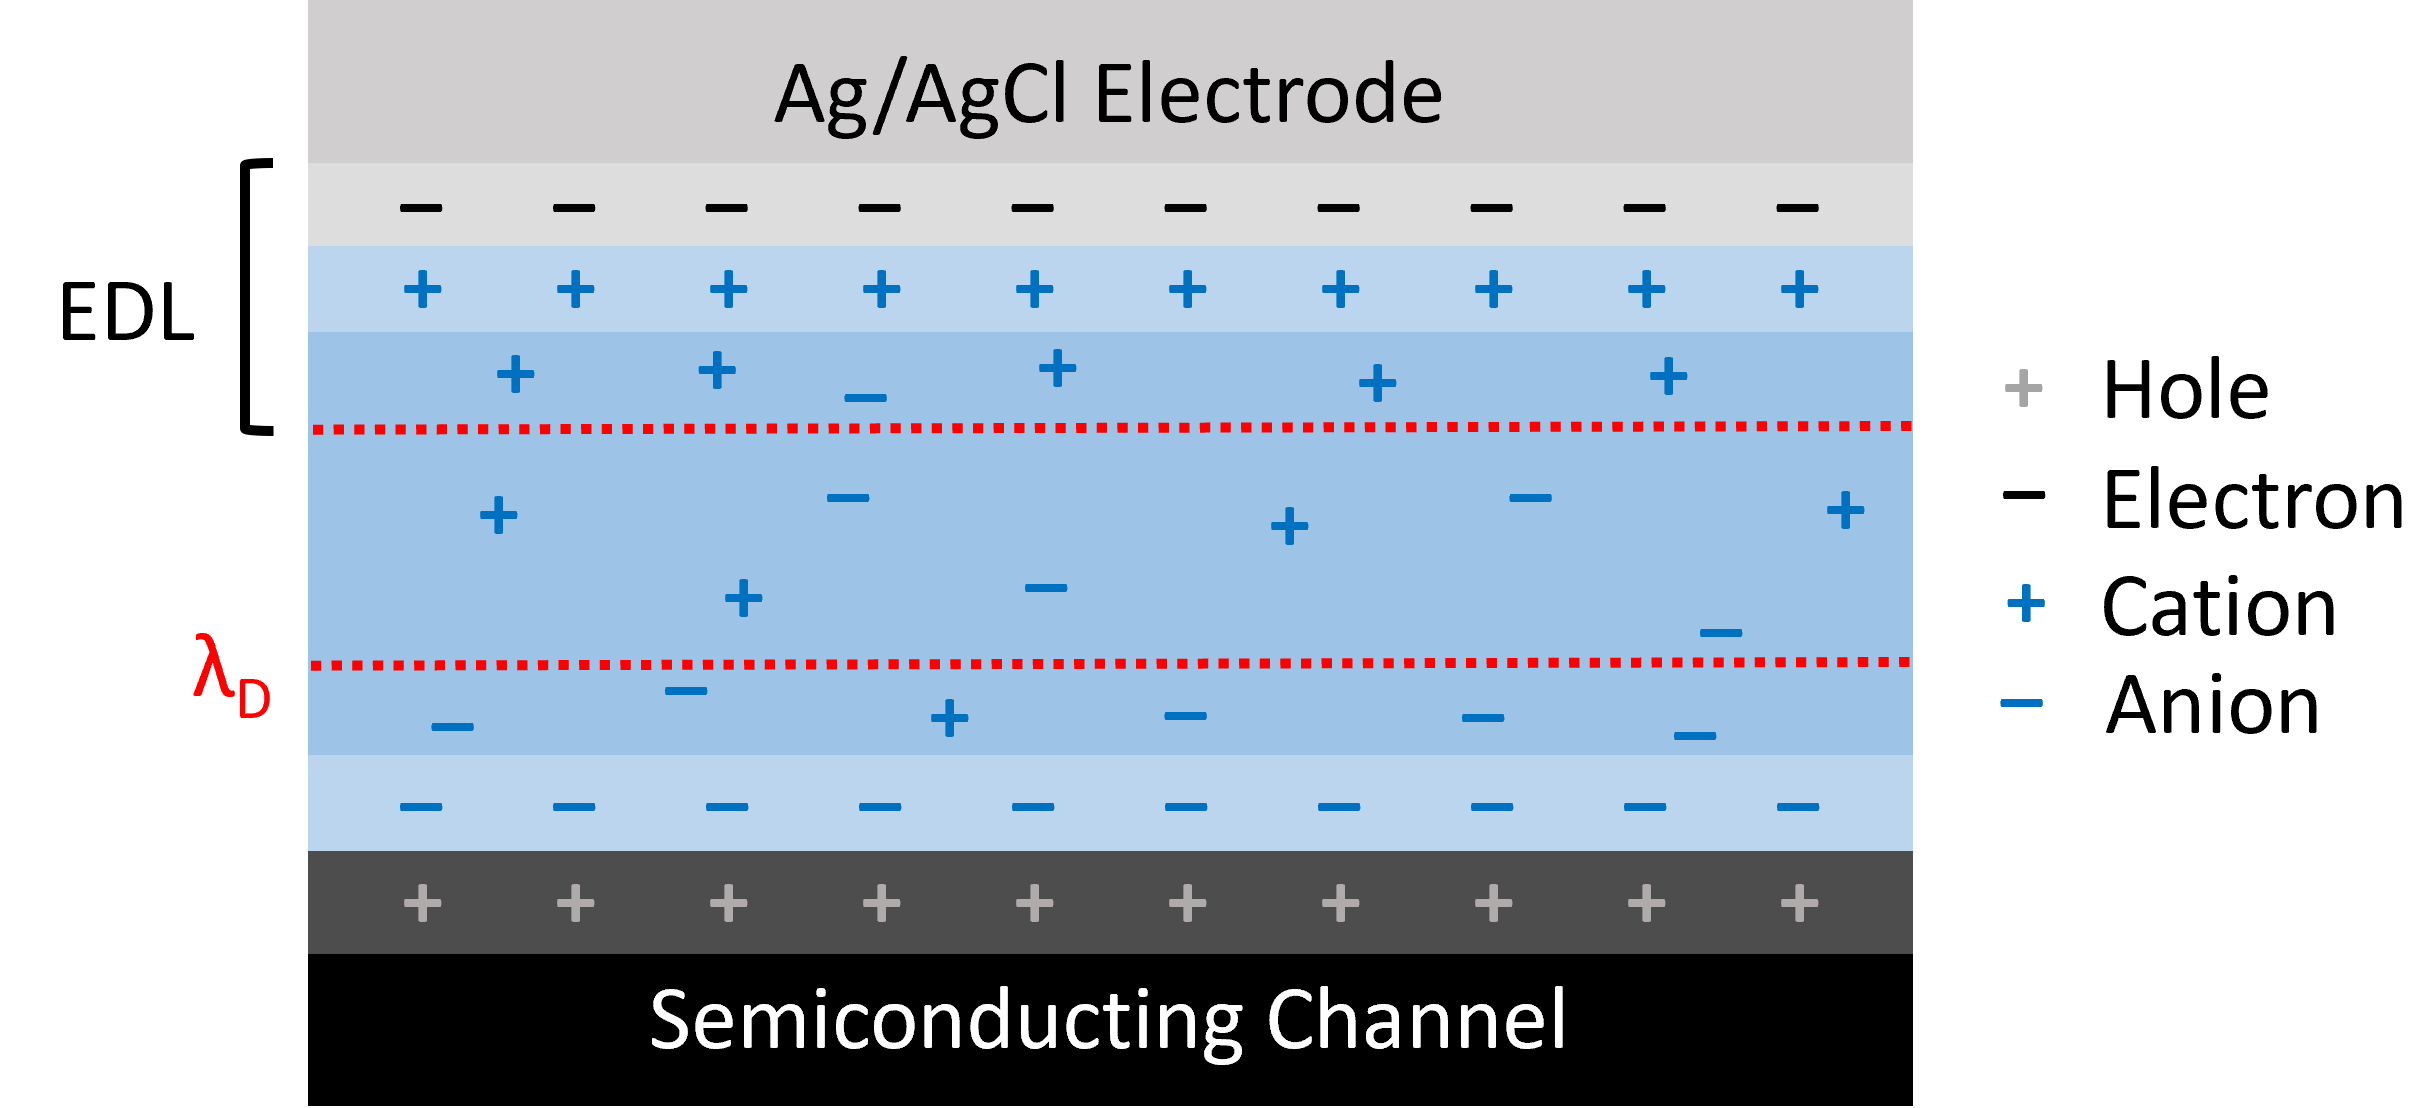
\includegraphics[width=0.7\textwidth,height=\textheight]{figures/ch2/Debye-length-schematic-alt.png}

}

\caption[A diagram of an electric double layer between source and
liquid-gate electrodes.]{\label{fig-Debye-length}A diagram of the
formation of an electric double layer (EDL) under an applied voltage
between source and liquid-gate electrodes, with a \(p\)-type
semiconductor used for the channel thin-film. Electric double layers are
present at both the gate-electrolyte interface and
semiconductor-electrolyte interface.}

\end{figure}

The equation for Debye length \(\lambda_D\) in an electrolyte solution
is given by Equation~\ref{eq-debye-length}.

\begin{equation}\protect\hypertarget{eq-debye-length}{}{
\lambda_D = \sqrt{\frac{\epsilon_0\epsilon_rk_bT}{2N_Aq^2I}}
}\label{eq-debye-length}\end{equation}

Here, \(\epsilon_0\) is vacuum permittivity, \(\epsilon_r\) is the
relative permittivity of the electrolyte, \(k_b\) is the Boltzmann
constant, \(T\) is absolute temperature in K, \(N_A\) is the Avogadro
number, \(q\) is the elementary charge and \(I\) is ionic strength in
mmol L\(^{-1}\). When temperature is kept constant, \(\lambda_D\) only
depends on the ionic strength of the electrolyte and not on any
attributes of the gate electrode or channel
\autocite{Stern2007,Shkodra2021}. Successive dilutions of a particular
electrolyte will increase the Debye length: for \(1 \times\) PBS,
\(\lambda_D\) is \(\sim\) 1 nm, for \(0.1 \times\) PBS, \(\lambda_D\) is
\(\sim\) 2 nm, for \(0.01 \times\) PBS \(\lambda_D\) is \(\sim\) 8 nm
and so on. This means gate capacitance is directly dependent on the
electrolyte used and its concentration
\autocite{Kireev2017,Shkodra2021}. A \(1 \times\) PBS electrolyte gives
a gate capacitance several orders of magnitude larger than that of a
SiO\(_2\) back-gate. A larger capacitance significantly increases the
effect of electrostatic gating on the channel current, often described
as increased electrostatic coupling between gate and channel. A
liquid-gated device with low Debye length will therefore be highly
sensitive to electrostatic changes across a small voltage range
\autocite{Heller2010,Ohno2015,Kireev2017,Yao2021}.

However, a decreased Debye length also has disadvantages for sensing.
Electrostatic potentials outside of the electrolyte-channel electrical
double layer are effectively screened from the channel. Electrical
double layers will also form around charged receptors within the
solution. The combined screening effect means signals due to potential
changes in charged biomolecules within the bulk electrolyte will have no
effect on gating of the channel, and therefore no effect on \(I_d\).
Interactions between the analyte and any receptor element must therefore
occur within the Debye length, and so a tradeoff exists between channel
sensitivity and the size of the sensitive region above the channel. Many
medium or large proteins will require a relatively dilute electrolyte
for analyte capture to be detected by the channel, which may not reflect
the intended environment for biosensor application
\autocite{Stern2007,Piccinini2018,Shkodra2021}. Other approaches to
increasing Debye length without reducing device sensitivity have
therefore also been trialled. One approach involves attaching a layer of
polyethylene glycol polymer (PEG) to the channel, limiting the approach
of counterions. This increases Debye length at the electrolyte-channel
interface while preserving the capacitance of the electrolyte-gate
interface, keeping device sensitivity relatively high
\autocite{Gao2016,Filipiak2018,Kesler2020,Albarghouthi2022}.

\hypertarget{electrical-characterisation}{%
\subsection{Electrical
Characterisation}\label{electrical-characterisation}}

\begin{figure}

{\centering 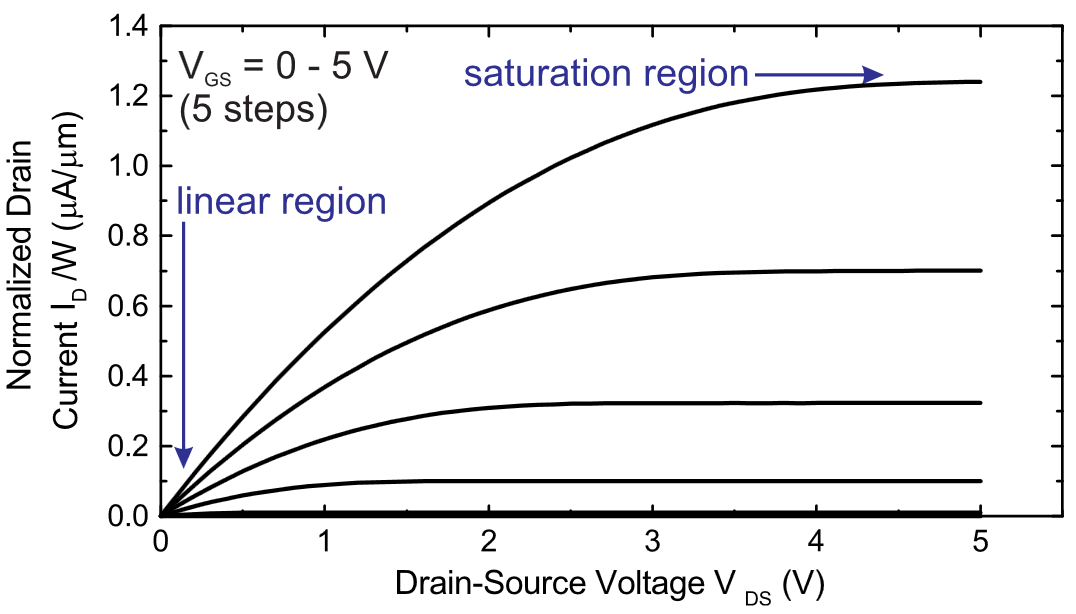
\includegraphics[width=0.65\textwidth,height=\textheight]{figures/ch2/linear_region_edit.png}

}

\caption[The linear and saturation operation regimes of an \(n\)-type
metal oxide semiconductor thin-film
transistor.]{\label{fig-linear-region}The linear and saturation
operation regimes of an \(n\)-type metal oxide semiconductor thin-film
transistor, \(V_{t} \sim 0\) V. Current has been normalised with respect
to channel width (W). Reproduced with permission from
\autocite{Petti2016}. Copyright \(\copyright\) 2016 AIP Publishing.}

\end{figure}

The current-voltage plots of a given transistor are known as its
``characteristic curves''. The I-V curve of \(I_d\) against \(V_{ds}\)
at constant \(V_g\) is known as the ``source-drain'' or ``output''
characteristic curve, while \(I_d\) against \(V_g\) at constant
\(V_{ds}\) is known as the ``transfer'' characteristic curve at that
source-drain voltage \autocite{Kauffman2008,Petti2016,Shkodra2021}.
Applying a gate voltage \(V_g\) to the gate of an thin-film transistor
influences the amount and type of available charge carriers for
conduction \autocite{Avouris2007,Tran2016,Heller2009a}. In an ambipolar
transistor, a highly negative \(V_g\) will give rise to hole conduction,
and a highly positive \(V_g\) will give rise to electron conduction
\autocite{Avouris2007,Yao2021,Li2023}. The minimum \(V_g\) required to
turn the flow of current in a thin-film transistor ``on'' is referred to
as the threshold voltage \(V_t\)
\autocite{Petti2016,Shkodra2021,Li2023}. Threshold voltage is discussed
in more detail in Section~\ref{sec-electrical-characterisation-CNT}.
When \(|V_{ds}| < |V_g| - |V_t|\) while \(|V_g|>|V_t|\), the device is
in the linear regime. Here, \(V_{ds}\) is directly proportional to
\(I_{d}\), similar to an Ohmic resistor. When
\(|V_{ds}| > |V_g| - |V_t|\) and \(|V_g|>|V_t|\), the device is in the
saturation regime, where the relationship between \(V_{ds}\) and
\(I_{d}\) becomes non-linear \autocite{Petti2016,Shkodra2021,Li2023}.

\begin{figure}

\begin{minipage}[t]{0.03\linewidth}

{\centering 

\raisebox{-\height}{


\includegraphics{figures/(a).png}

}

}

\end{minipage}%
%
\begin{minipage}[t]{0.01\linewidth}

{\centering 

~

}

\end{minipage}%
%
\begin{minipage}[t]{0.45\linewidth}

{\centering 

\raisebox{-\height}{

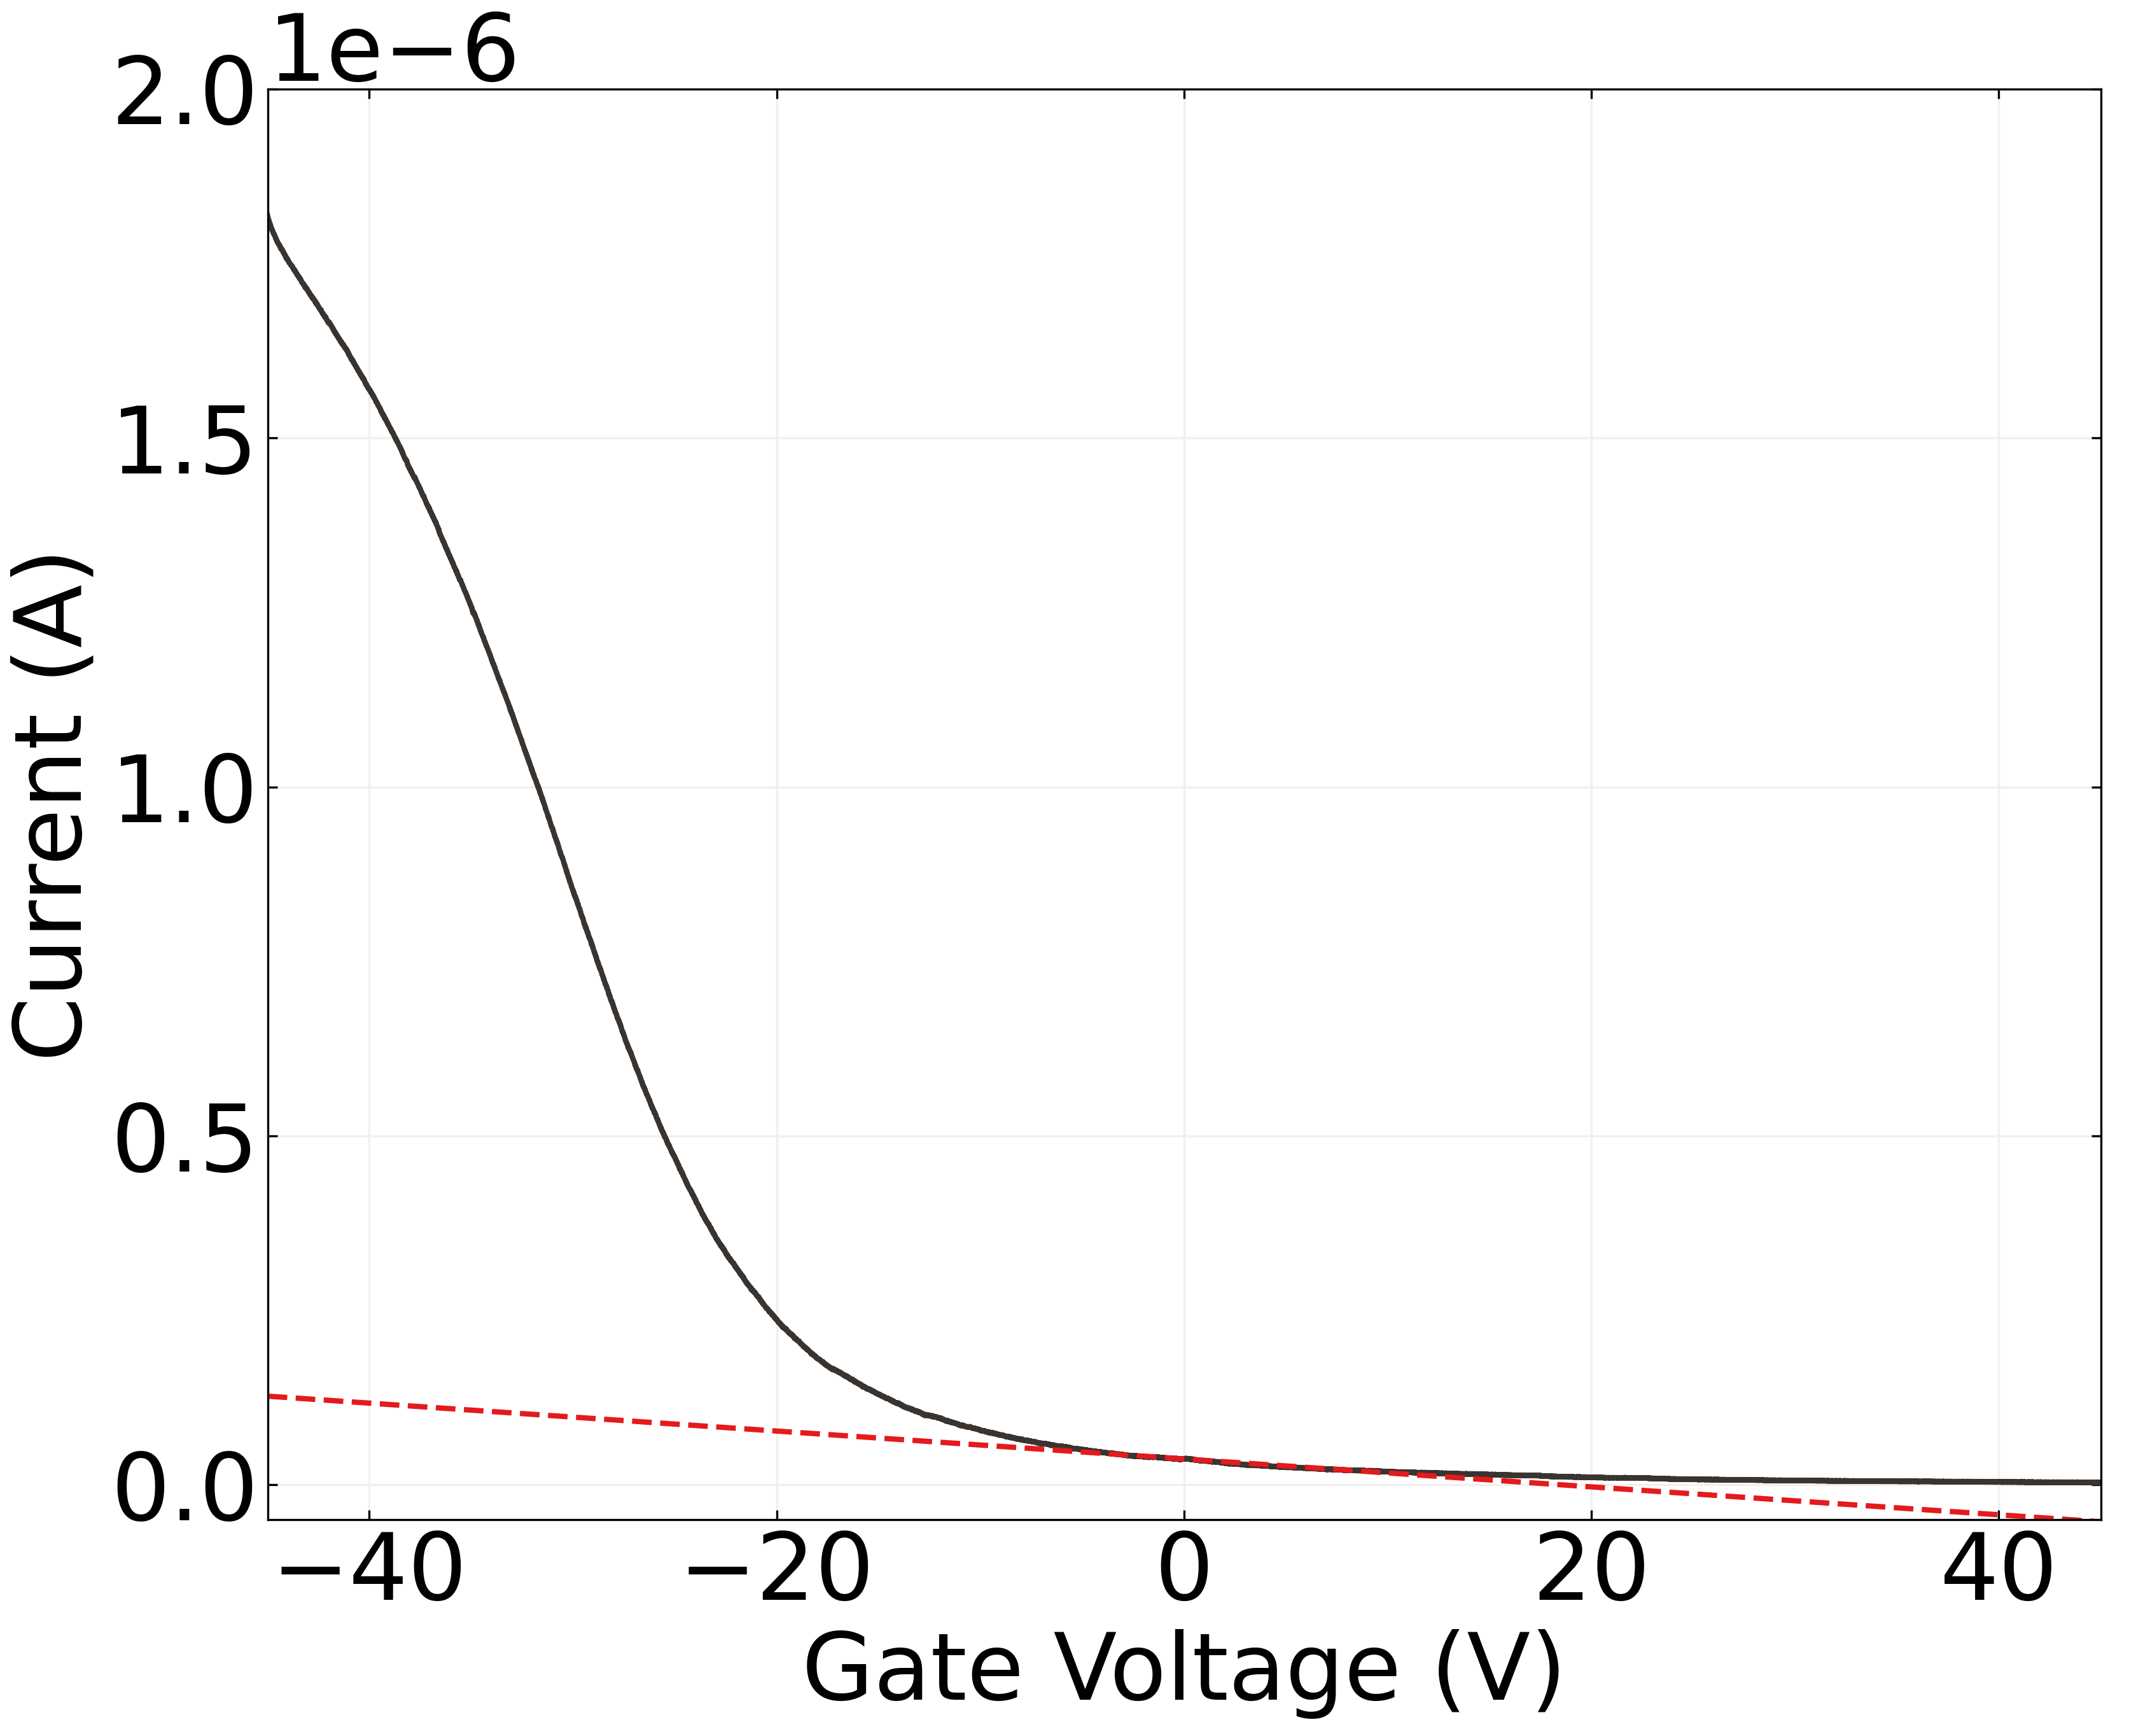
\includegraphics{figures/ch2/Q5C10ch8transconductance.png}

}

}

\end{minipage}%
%
\begin{minipage}[t]{0.01\linewidth}

{\centering 

~

}

\end{minipage}%
%
\begin{minipage}[t]{0.03\linewidth}

{\centering 

\raisebox{-\height}{


\includegraphics{figures/(b).png}

}

}

\end{minipage}%
%
\begin{minipage}[t]{0.01\linewidth}

{\centering 

~

}

\end{minipage}%
%
\begin{minipage}[t]{0.45\linewidth}

{\centering 

\raisebox{-\height}{

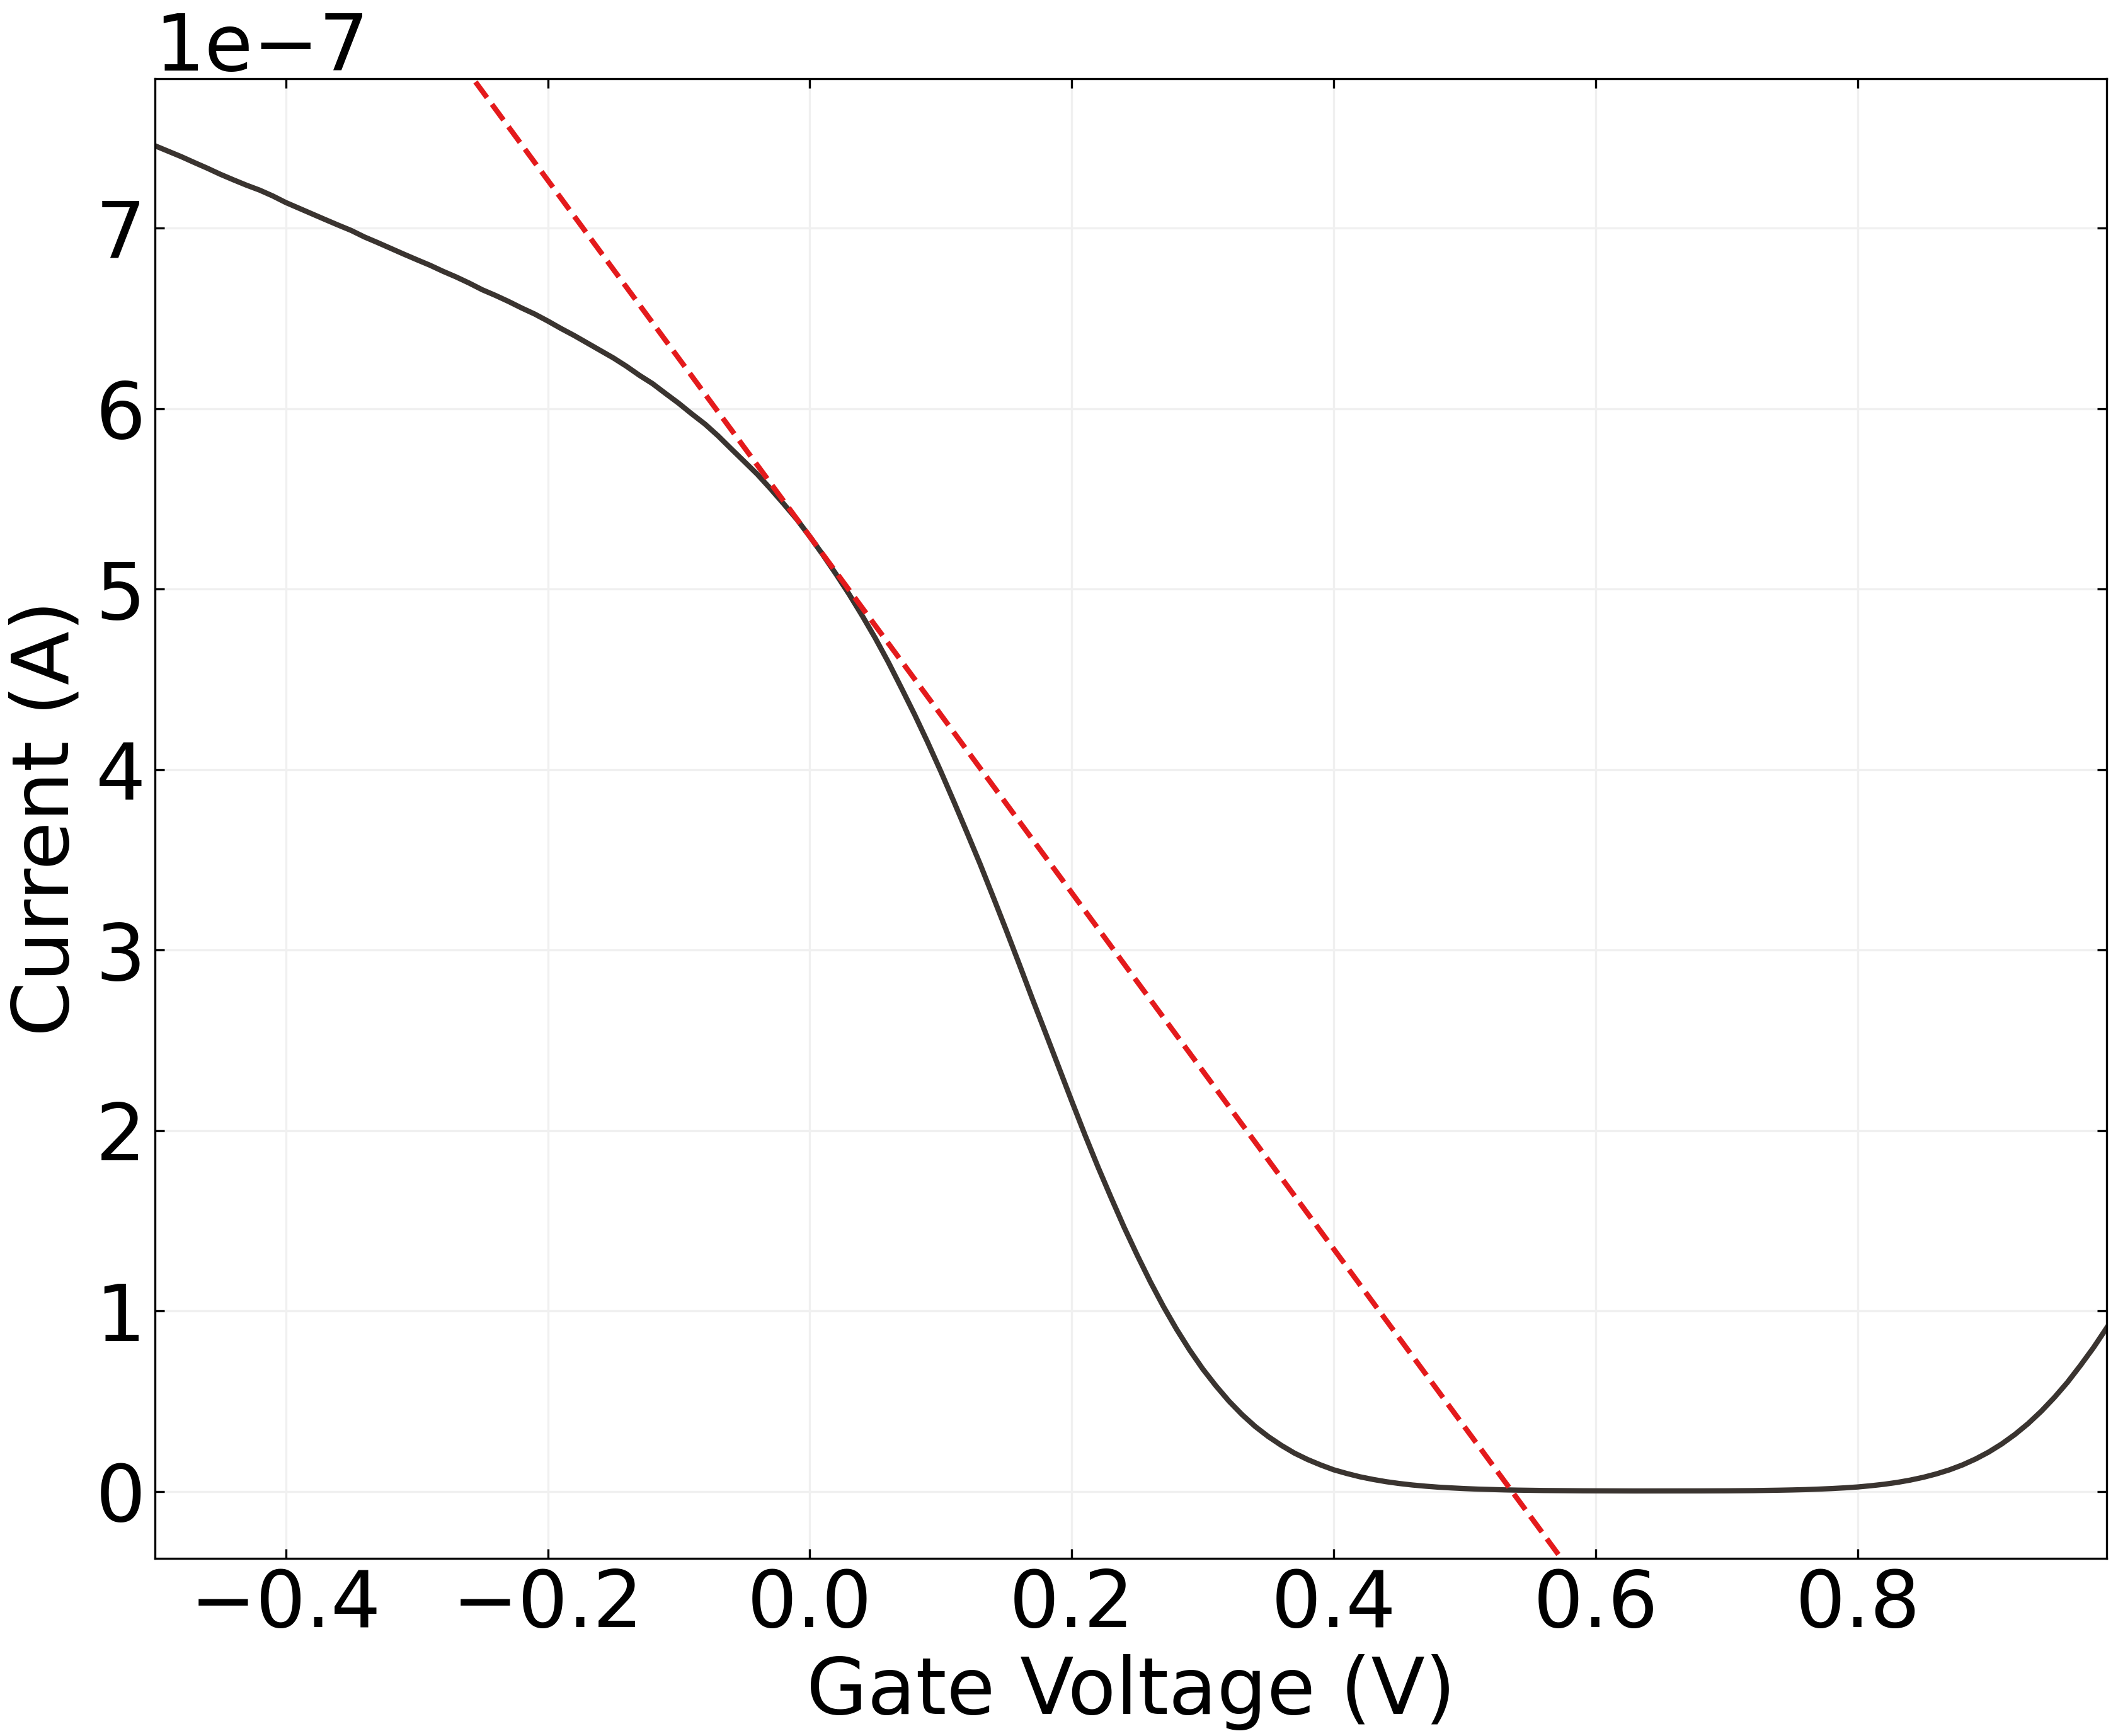
\includegraphics{figures/ch2/NTQ31C5ch1transconductance.png}

}

}

\end{minipage}%
%
\begin{minipage}[t]{0.01\linewidth}

{\centering 

~

}

\end{minipage}%
\newline
\begin{minipage}[t]{0.03\linewidth}

{\centering 

\raisebox{-\height}{


\includegraphics{figures/(c).png}

}

}

\end{minipage}%
%
\begin{minipage}[t]{0.01\linewidth}

{\centering 

~

}

\end{minipage}%
%
\begin{minipage}[t]{0.45\linewidth}

{\centering 

\raisebox{-\height}{

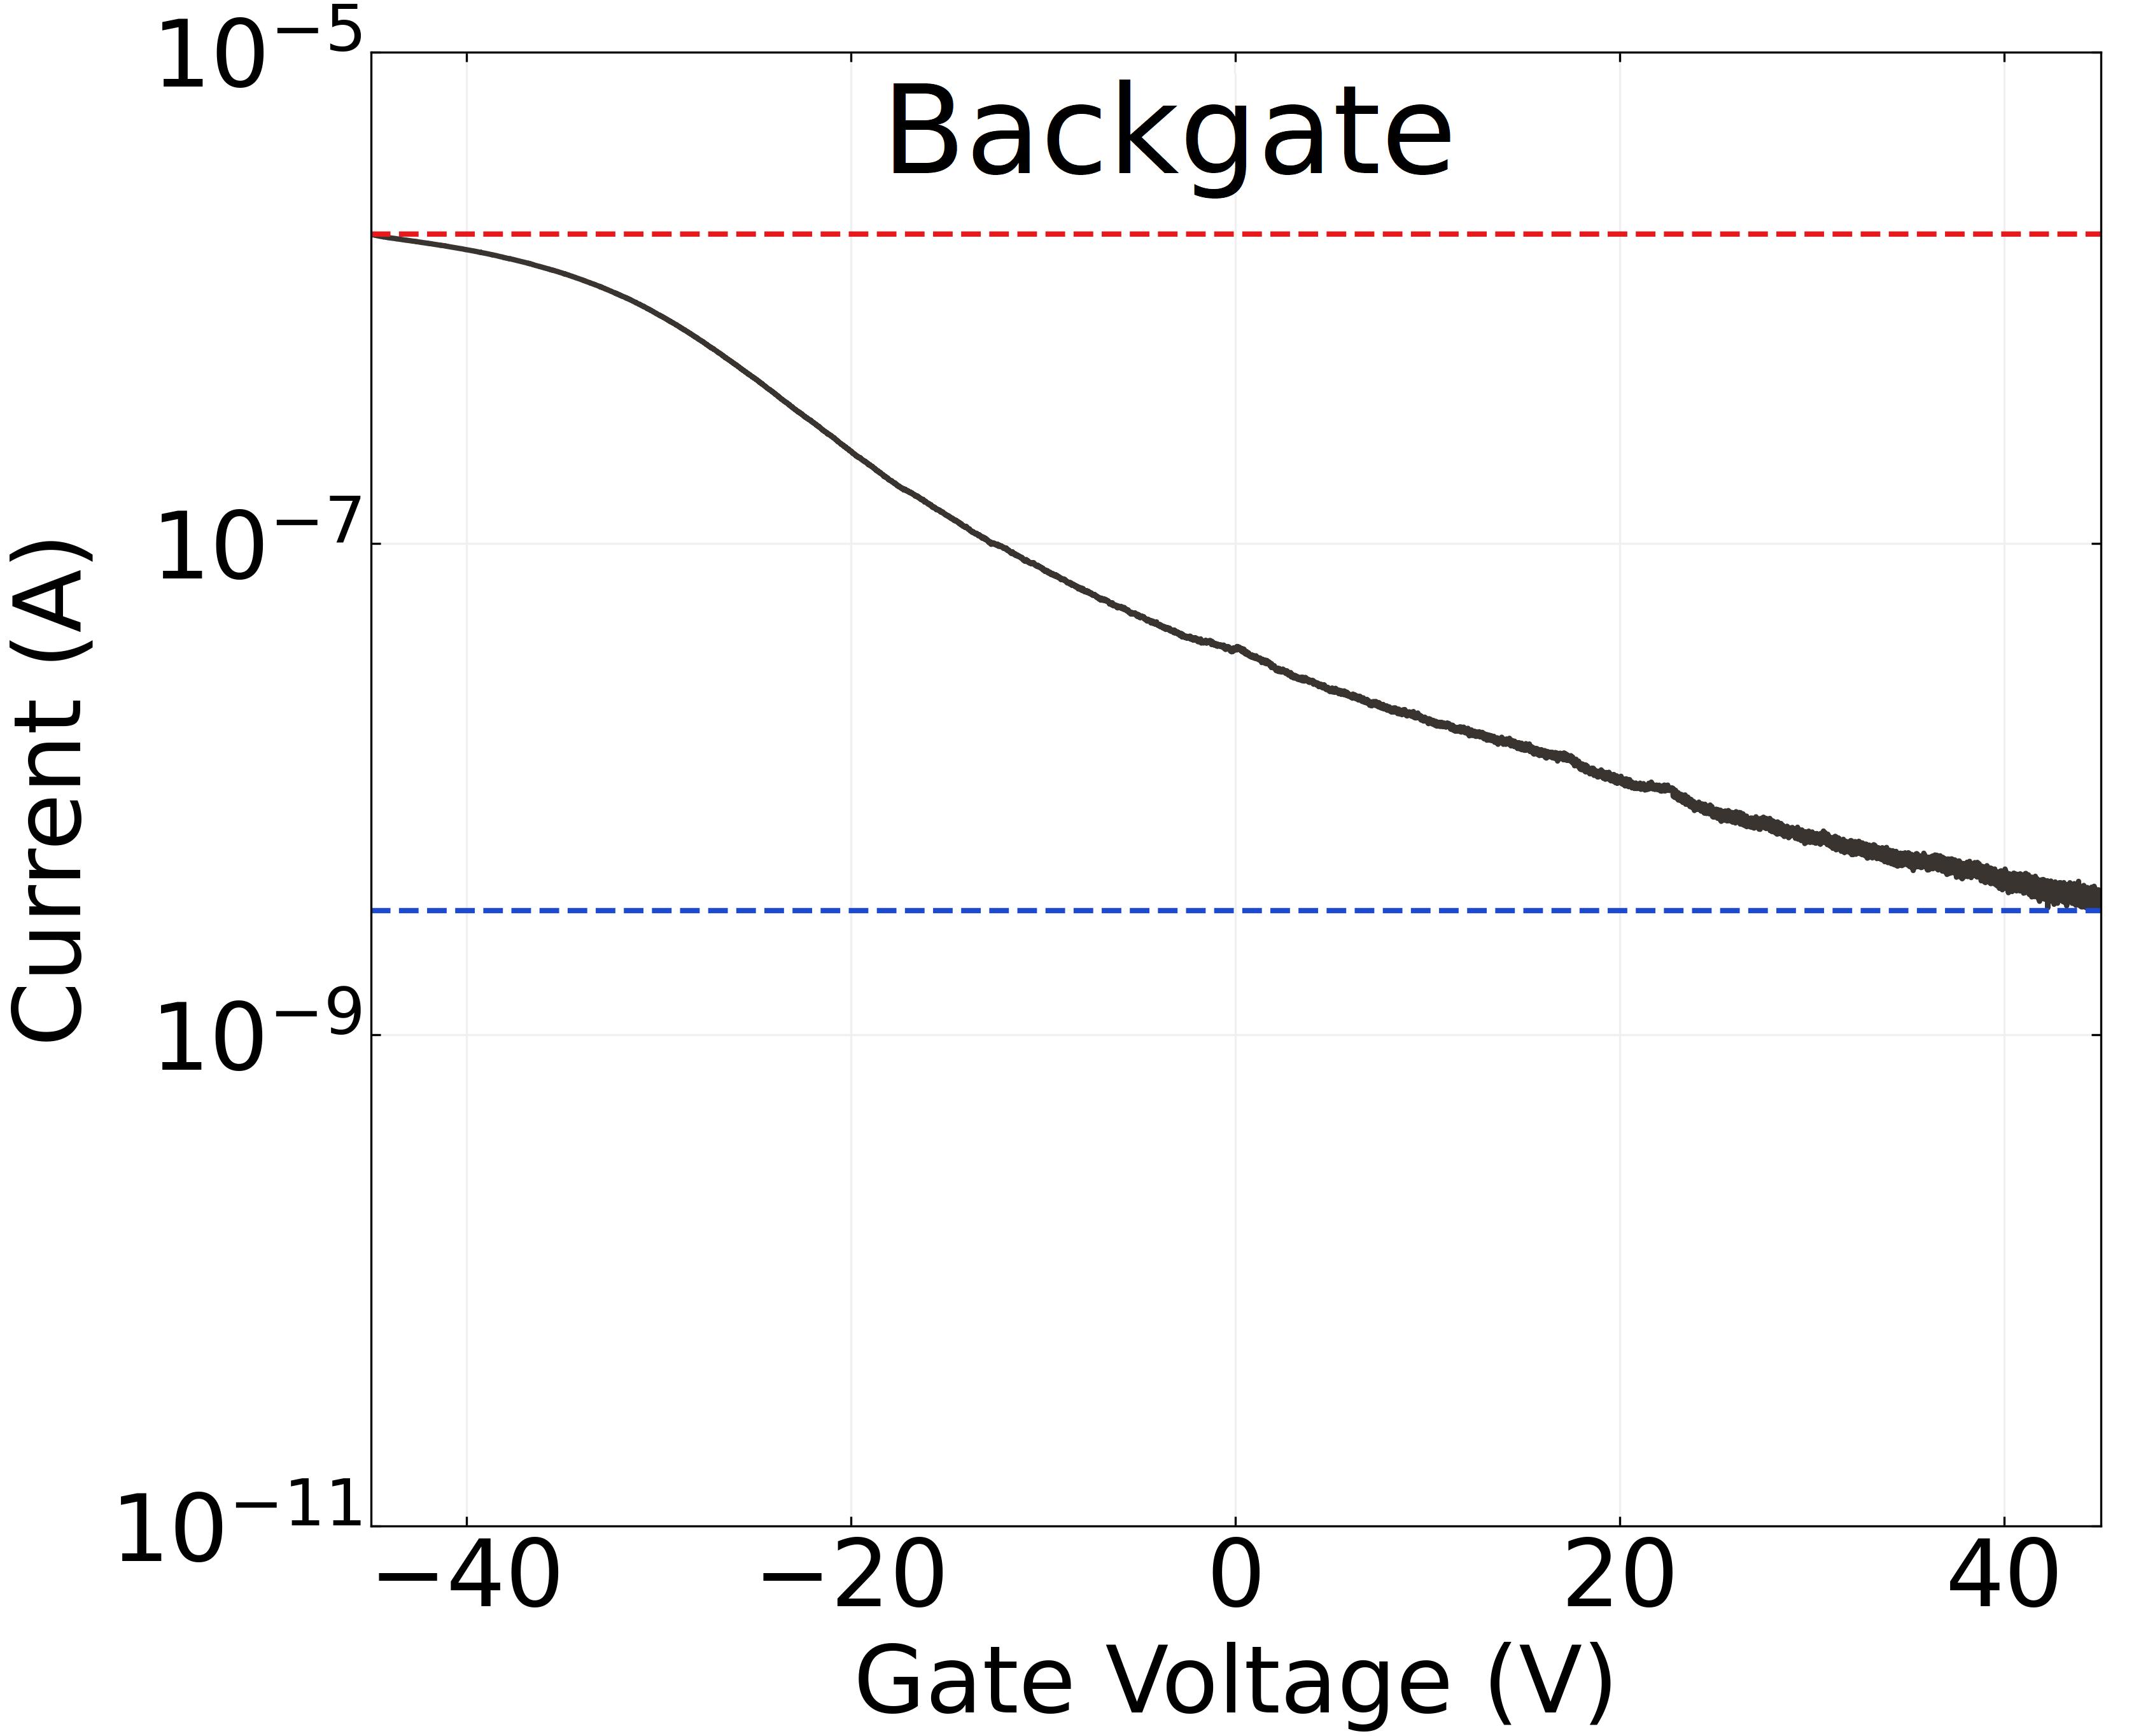
\includegraphics{figures/ch2/Q5C10ch8on_off_current.png}

}

}

\end{minipage}%
%
\begin{minipage}[t]{0.01\linewidth}

{\centering 

~

}

\end{minipage}%
%
\begin{minipage}[t]{0.03\linewidth}

{\centering 

\raisebox{-\height}{

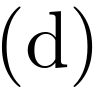
\includegraphics{figures/(d).png}

}

}

\end{minipage}%
%
\begin{minipage}[t]{0.01\linewidth}

{\centering 

~

}

\end{minipage}%
%
\begin{minipage}[t]{0.45\linewidth}

{\centering 

\raisebox{-\height}{

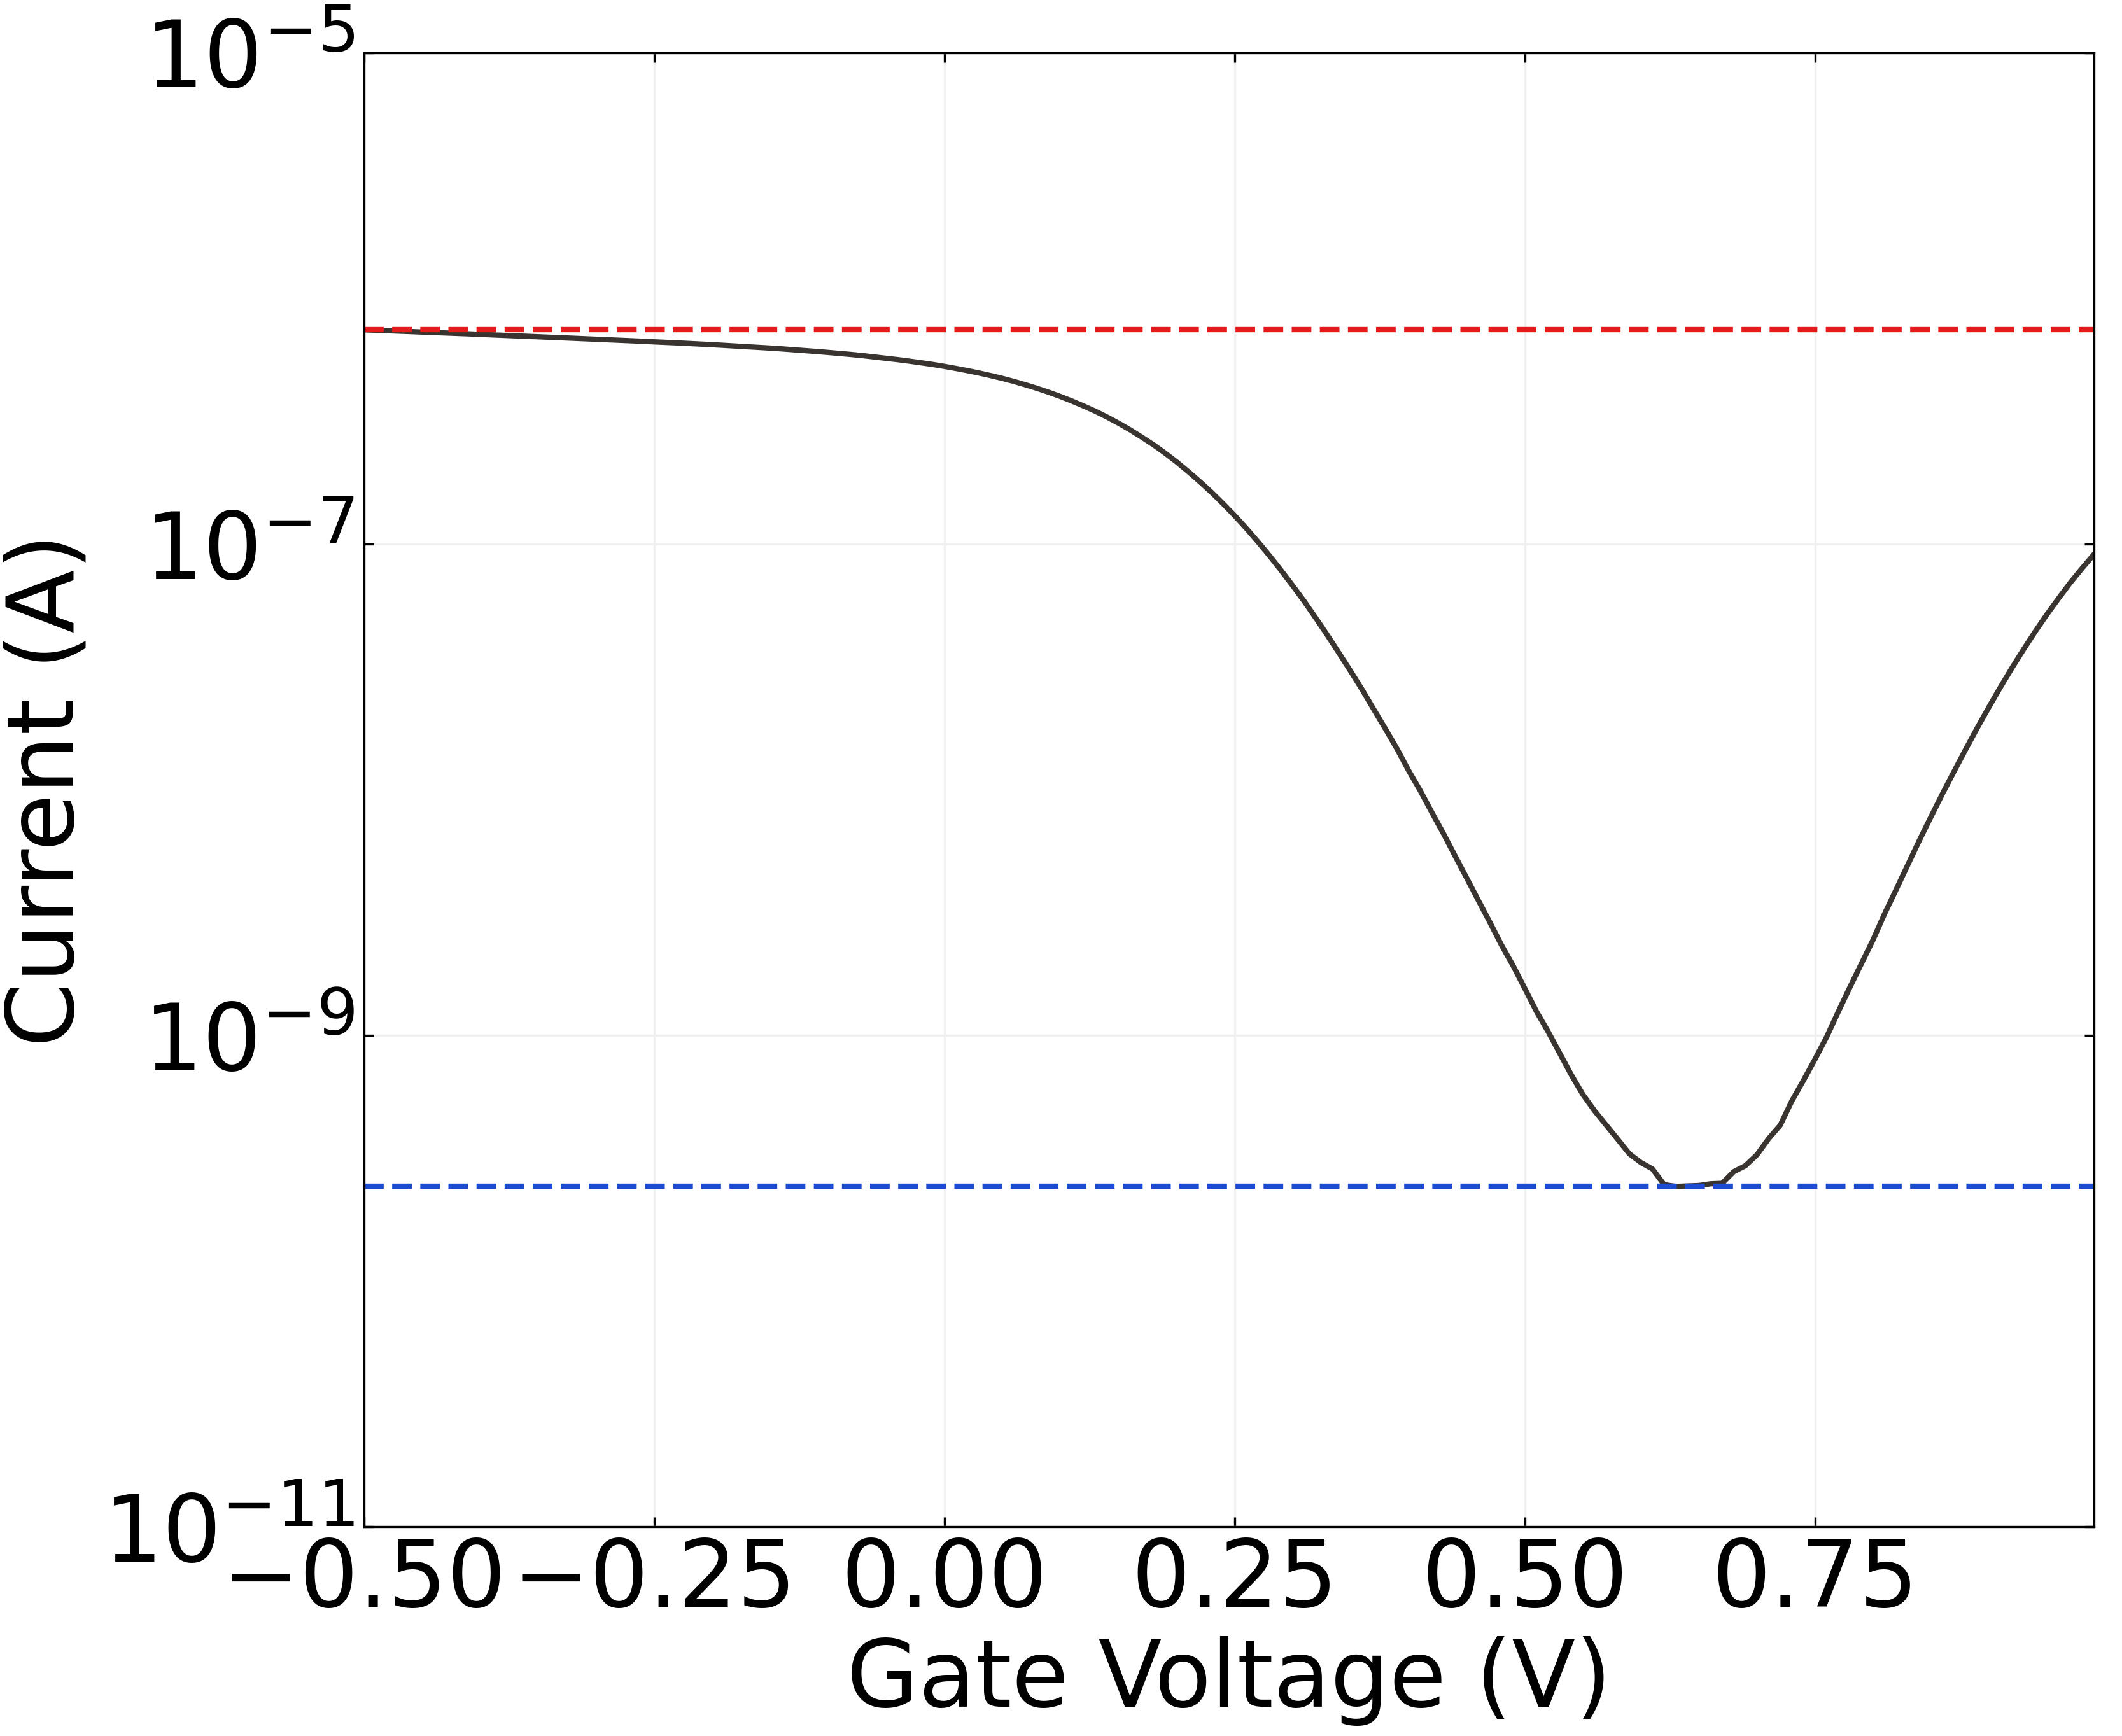
\includegraphics{figures/ch2/NTQ31C5ch1on_off_current.png}

}

}

\end{minipage}%
%
\begin{minipage}[t]{0.01\linewidth}

{\centering 

~

}

\end{minipage}%

\caption[Examples of field-effect transistor transfer characteristics
when back-gated and liquid-gated, showing transconductance, on-current
and off-current.]{\label{fig-gating-transfer}Examples of field-effect
transistor transfer characteristics taken at \(V_{ds}\) = 100 mV using
two carbon nanotube network device channels fabricated in the same
manner. A linear scale is used in (a) and (b), while a logarithmic scale
is used in (c) and (d). The curves in (a) and (c) are from a backgated
channel, while the curves in (b) and (d) are from a liquid-gated
channel. The linear fit with gradient corresponding to transconductance
at \(V_g\) = 0 V is shown in (a) and (b) with a dotted red line. The
approximate on current in (c) and (d) is shown with a red horizontal
line, while the off current is shown with a blue horizontal line.}

\end{figure}

The linear and saturation regions for a metal oxide thin-film transistor
are shown in Figure~\ref{fig-linear-region}. In this thesis, constant
\(V_g\) measurements from thin-film transistors were typically taken
when \(V_{ds}\) was small and the TFT was in the linear operation
regime. Figure~\ref{fig-gating-transfer} (a) and (c) show back-gated
transfer characteristics of a thin-film transistor, and
Figure~\ref{fig-gating-transfer} (b) and (d) show liquid-gated TFT
transfer characteristics. The back-gated device exhibits unipolar
behaviour, where the transistor conducts in only one direction along the
\(I_d - V_g\) curve, while the liquid-gated device exhibits ambipolar
behaviour, where conduction occurs along both directions of the curve.
The liquid-gated device is also able to traverse a wide range of
currents over a much more limited voltage interval than the back-gated
device. A variety of quantitative parameters or figures of merit can be
extracted from the transfer characteristics of a thin-film transistor
\autocite{Petti2016}. Transconductance and on-off ratio are discussed
below, while threshold voltage and subthreshold swing are discussed for
the carbon nanotube network case in
Section~\ref{sec-electrical-characterisation-CNT}.

One of the most important figures of merit which can be extracted from
the transfer characteristic curve of a thin-film FET is the on-off
current ratio, the ratio of the current through a device when the
transistor is gated fully ``on'', \(I_{on}\), to the current \(I_{off}\)
when gated fully ``off''. \autocite{Kauffman2008,Petti2016,Shkodra2021}.
Having a low off current is desirable as it corresponds to low power
consumption by the transistor \autocite{Rouhi2010}. In
Figure~\ref{fig-gating-transfer} (a), there is a clear on regime at
large negative voltages and an off regime at large positive voltages.
Although the transfer curve never completely flattens in each direction,
\(I_{on}\) can be reasonably estimated with the highest current
obtained, while \(I_{off}\) can be estimated from the lowest current
reading. In an ambipolar FET, such as that shown in
Figure~\ref{fig-gating-transfer} (b), the off current can be defined as
the minimum current during the transfer sweep, where the majority
carrier transitions from being holes to electrons or \emph{vice versa}
\autocite{Petti2016,Zheng2017}. For the backgated channel shown in
Figure~\ref{fig-gating-transfer} (a), the on-off ratio
\(I_{on}/I_{off}\) is \(\sim\) 700, while for the liquid-gated device in
Figure~\ref{fig-gating-transfer} (b), \(I_{on}/I_{off} \sim 3000\).
These values are comparable to those found in the literature
\autocite{Avouris2007,Kauffman2008,Heller2010}. The superior on-off
ratio is a significant advantage of the liquid-gated configuration
\autocite{Shkodra2021}.

In the linear regime, transconductance at a specific gate voltage is
given by \(g_m = |dI_{d}/dV_g|\). Transconductance indicates how
responsive the device is to electrostatic gating at a given gate
voltage. In other words, when \(g_m\) is large, small changes in \(V_g\)
can significantly modulate channel current \(I_d\), which is useful for
sensing \autocite{Heller2009a,Ohno2015,Kireev2017}. Transconductance at
a given gate voltage is also proportional to the mobility (movement) of
charge carriers in the device channel, and therefore depends on the
scattering properties of the material
\autocite{Rouhi2010,Petti2016,Li2023}. The transconductance at a
specific gate voltage can be found from performing a linear fit in a
small region around that voltage on the transfer curve. Linear fits for
transconductance at \(V_g = 0\) V, the operating voltage used for
sensing in this thesis, are shown for a back-gated device in
Figure~\ref{fig-gating-transfer} (a), and a liquid-gated device in
Figure~\ref{fig-gating-transfer} (b). The corresponding transconductance
values of \(g_m\) = 0.002 µS and \(g_m\) = 1 µS respectively. The
difference of several orders of magnitude between back-gated and
liquid-gated transconductance corresponds to the difference of several
orders of magnitude between back and liquid-gated gate capacitance
\autocite{Tran2016,Shkodra2021}. The ability to achieve high
transconductance at relatively low voltage is important for the creation
of low power sensors, which is another advantage of the liquid-gated
setup.

``Application of higher voltages to the gate in both the liquid-gate and
back-gate cases can result in significant leakage currents through the
gate. These currents mean that the insulating layer at the gate
producing the capacitive effect no longer acts as an insulator,
adversely affecting transistor behaviour and contributing to sensor
drift that may be mistaken for signal responses to analyte
\autocite{Noyce2019,Shkodra2021,Albarghouthi2022}. In the case of
back-gated devices, gate leakage occurs due to conduction through the
oxide dielectric. If the gate voltage produces an electric field
exceeding the dielectric strength of the oxide, dielectric breakdown can
occur, where the oxide layer no longer acts as an insulator. Breakdown
results from voltage-induced oxygen vacancies in the SiO\(_2\) lattice
forming a conductive path through the insulator \autocite{Padovani2017}.
Irreversible breakdown occurred at \(\sim\) 50 V for the back-gated
channel in Figure~\ref{fig-gating-transfer}. In the liquid-gated case,
the electrolyte used determines the appropriate voltage range for
electrical characterisation, since excessive voltages will induce redox
reactions. For water-based electrolytes, gate voltages must be kept
within the \(\pm\) 1 V range \autocite{Wang2010,Ohno2015,Shkodra2021}.
In normal operation, gate current should appear negligible on a linear
scale, as shown in Figure~\ref{fig-gating-hysteresis}.

\begin{figure}

\begin{minipage}[t]{0.03\linewidth}

{\centering 

\raisebox{-\height}{


\includegraphics{figures/(a).png}

}

}

\end{minipage}%
%
\begin{minipage}[t]{0.01\linewidth}

{\centering 

~

}

\end{minipage}%
%
\begin{minipage}[t]{0.45\linewidth}

{\centering 

\raisebox{-\height}{

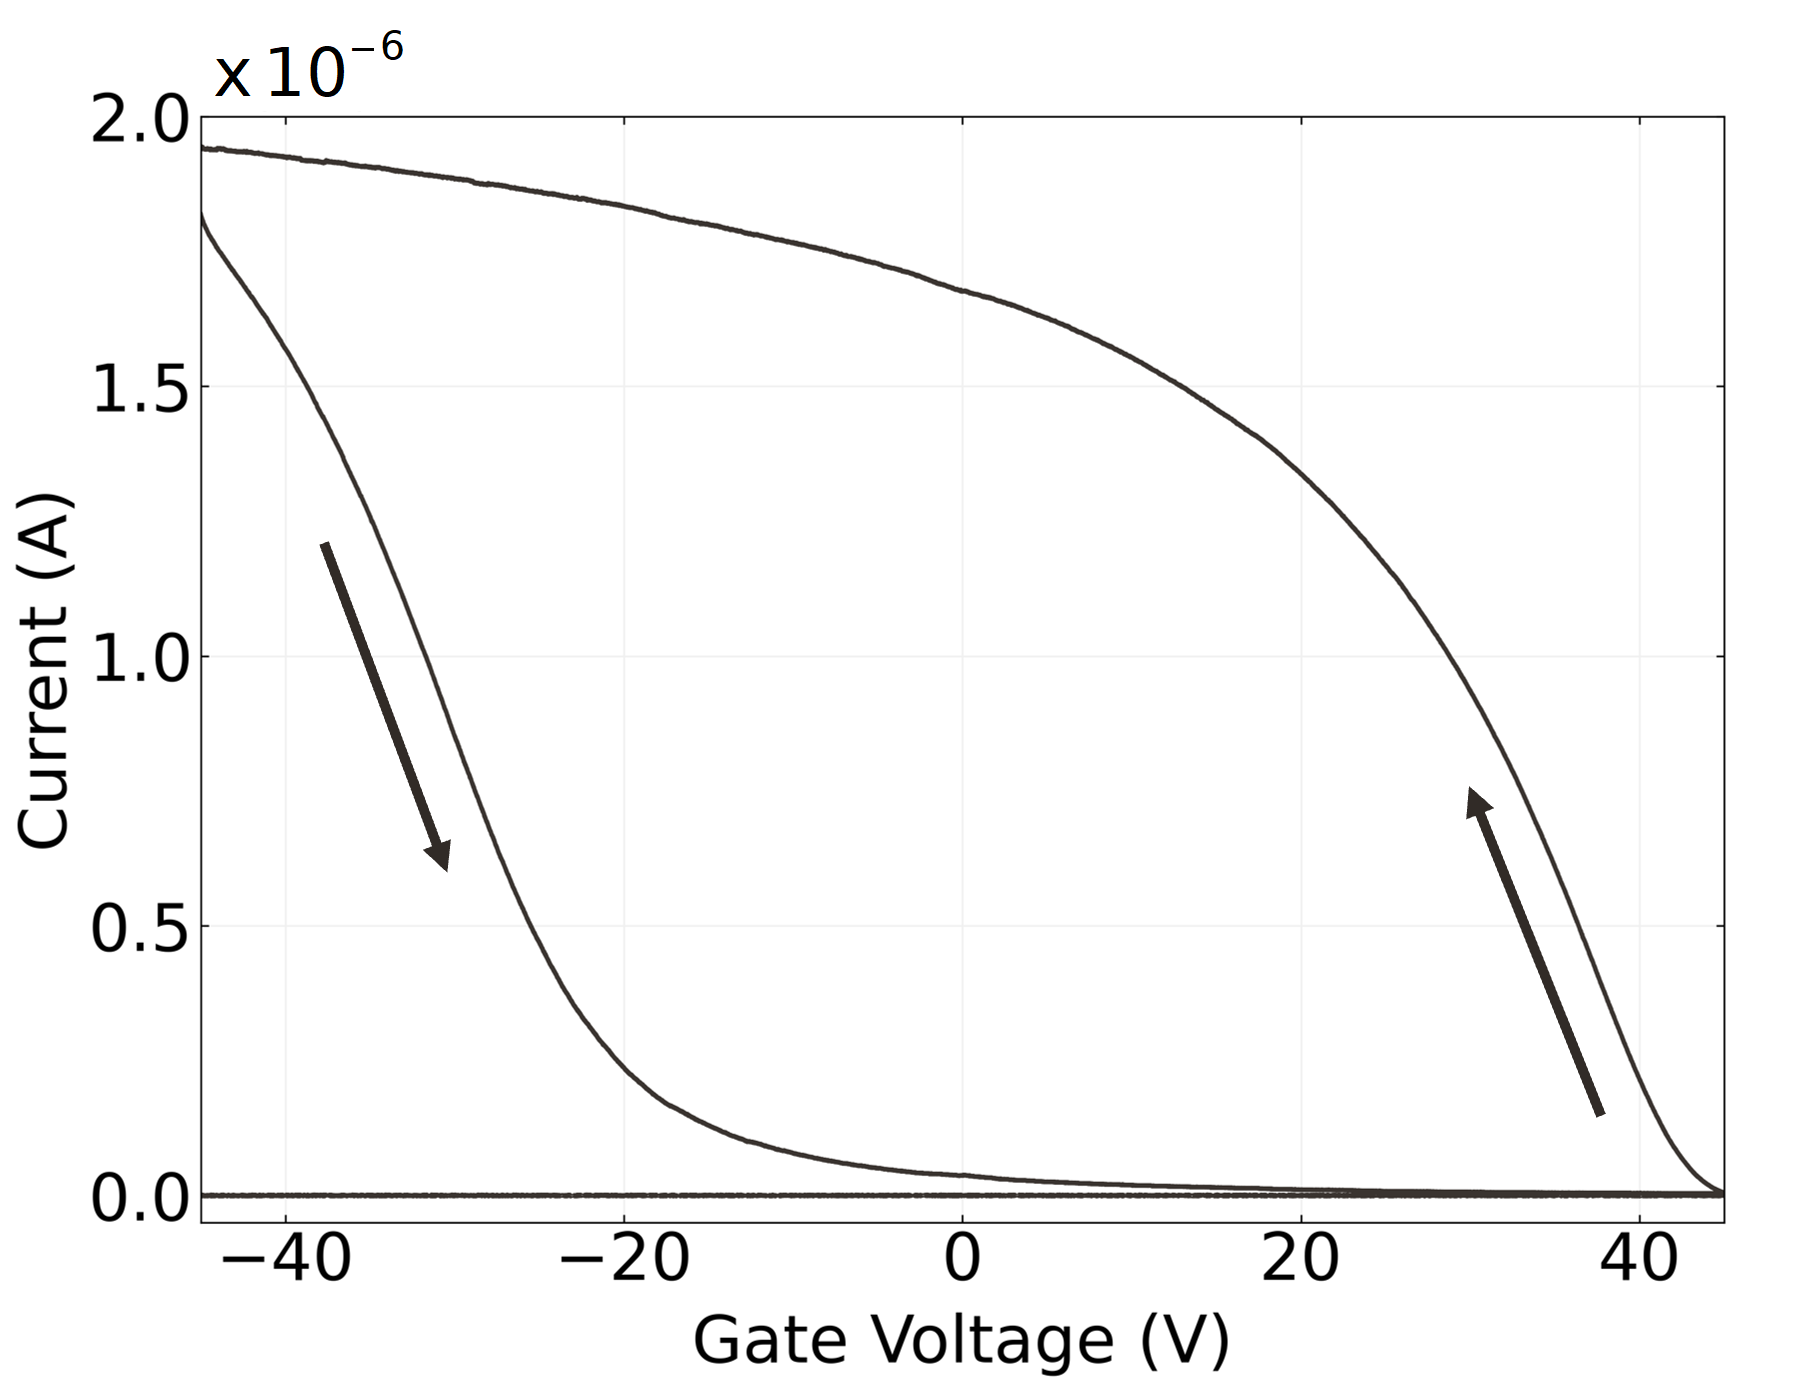
\includegraphics{figures/ch2/Q5C10_hysteresis.png}

}

}

\end{minipage}%
%
\begin{minipage}[t]{0.01\linewidth}

{\centering 

~

}

\end{minipage}%
%
\begin{minipage}[t]{0.03\linewidth}

{\centering 

\raisebox{-\height}{


\includegraphics{figures/(b).png}

}

}

\end{minipage}%
%
\begin{minipage}[t]{0.01\linewidth}

{\centering 

~

}

\end{minipage}%
%
\begin{minipage}[t]{0.45\linewidth}

{\centering 

\raisebox{-\height}{

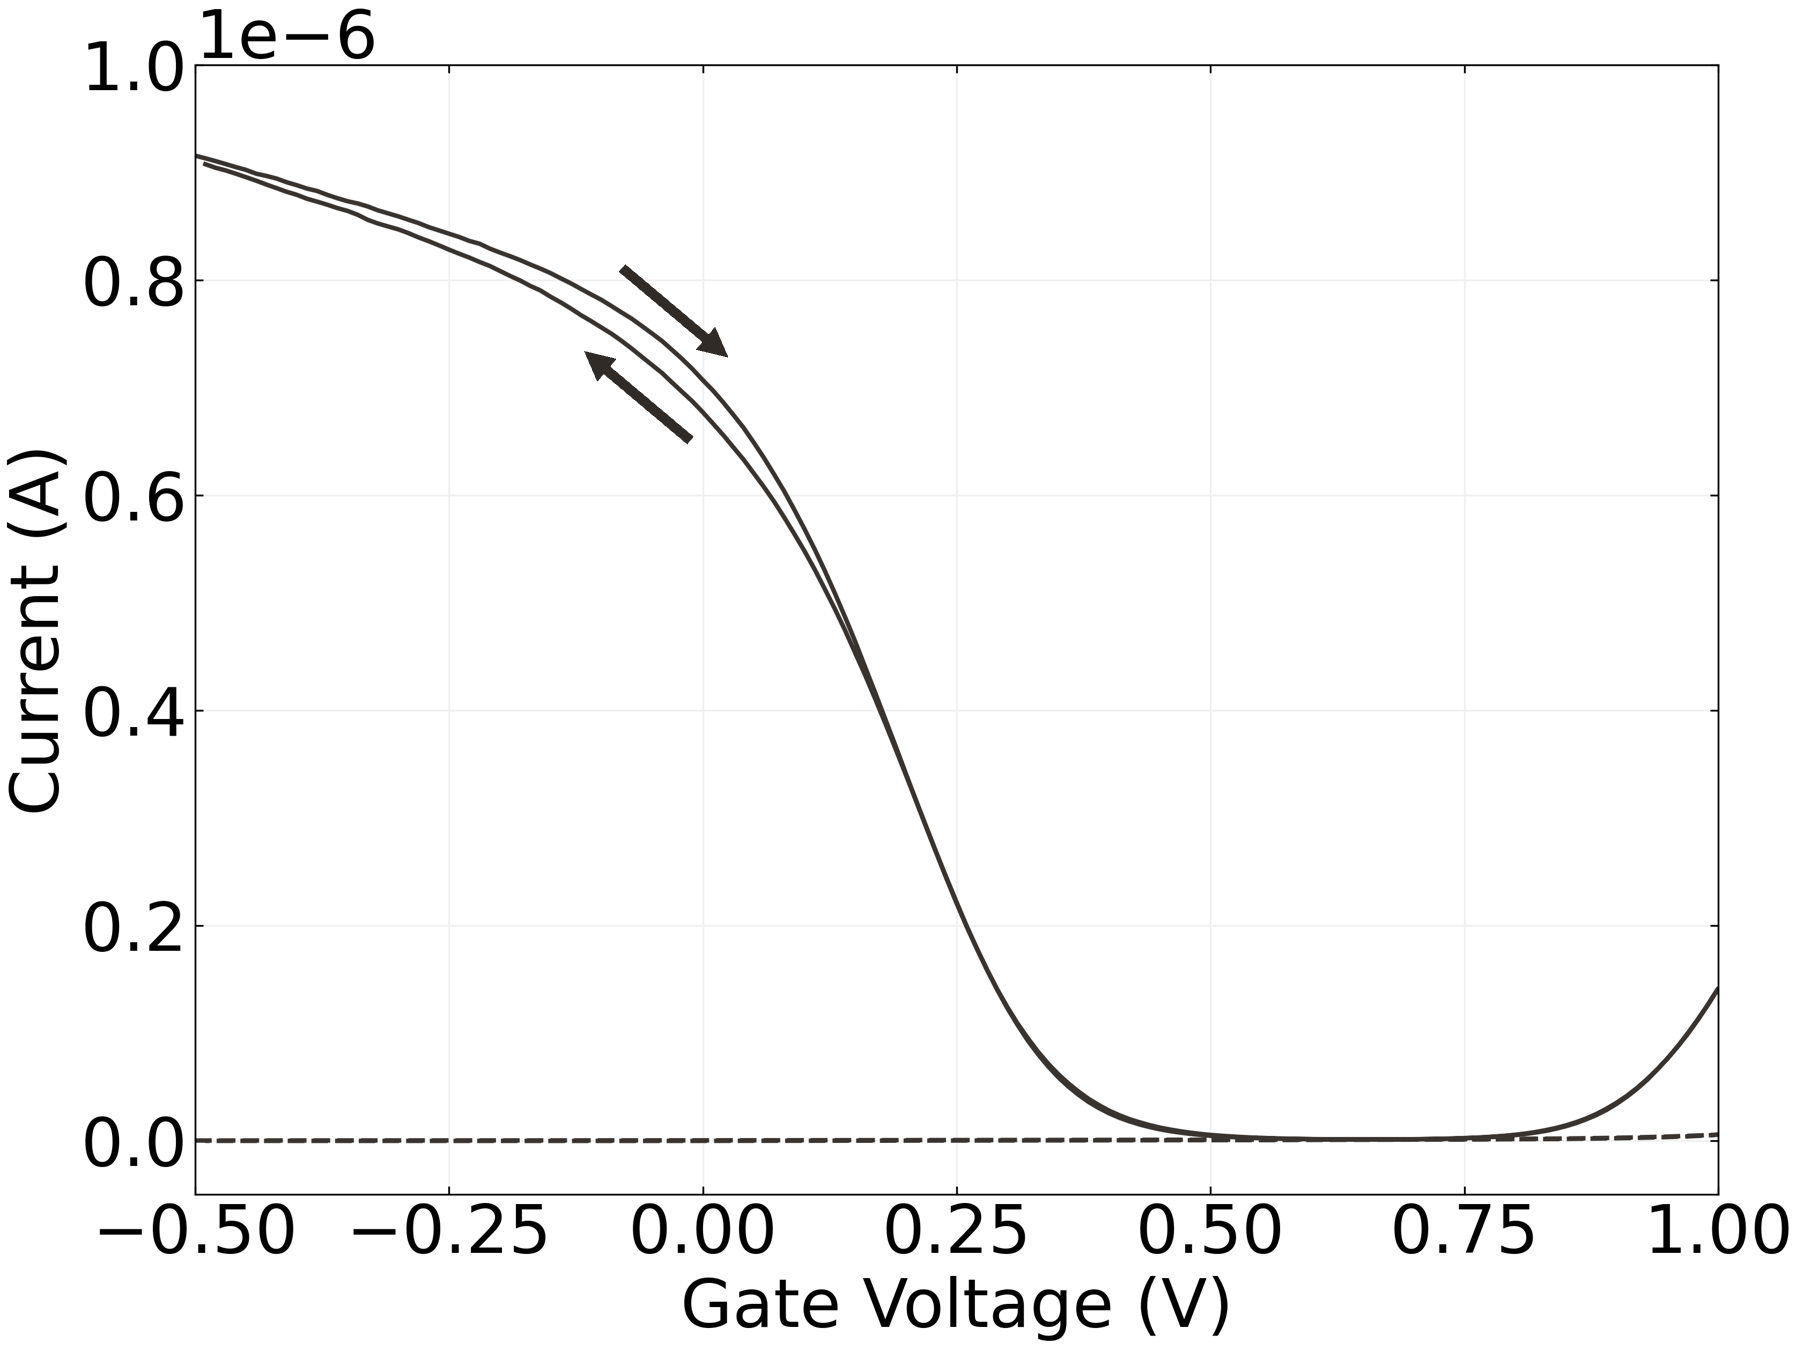
\includegraphics{figures/ch2/NTQ31C5_hysteresis.png}

}

}

\end{minipage}%
%
\begin{minipage}[t]{0.01\linewidth}

{\centering 

~

}

\end{minipage}%

\caption[Field-effect transistor transfer characteristics of back-gated
and liquid-gated device channels showing
hysteresis.]{\label{fig-gating-hysteresis}Field-effect transistor
transfer characteristics taken at \(V_{ds}\) = 100 mV from two different
device channels on a linear scale. Forward and reverse sweeps are shown
for the back-gated case (a) and the liquid-gated case (b), with the
direction of each sweep indicated by an arrow. A sweep rate of
\(V_{ds}\) = 10 mV/sample was used for both transfer curves. The gate
current measured during each sweep is also shown with a dotted line.}

\end{figure}

Thin-film transistor devices typically exhibit some degree of
hysteresis, where the history of channel current affects future current
behaviour. Hysteresis in carbon nanotube and graphene field-effect
transistors is a result of filling or emptying of slow-discharge charge
traps in the channel environment. These charge traps effectively dope
the SiO\(_2\) insulator or the insulator-channel interface, which
results from gate bias stress or dopant adsorption
\autocite{McEuen2002,Kim2003,Wang2010,Bartolomeo2011,Bargaoui2018,Peng2018}.
A capacitive gating effect from charged ions also contributes to
hysteresis, from the use of a electrolyte-gated environment or from
charged surface contamination \autocite{Wang2010,Yao2021}. Due to
hysteresis, sweeping \(V_g\) forwards across a set voltage range will
result in a different \(I_d - V_g\) characteristic curve than
subsequently sweeping over \(V_g\) in the reverse direction. Hysteresis
depends on the voltage range used for characterisation, the sweep rate
and the environment of the transistor channel
\autocite{Kim2003,Wang2010}. The effect of hysteresis on \(I_d\) when
sweeping gate voltage is shown in Figure~\ref{fig-gating-hysteresis}.
The measured hysteresis is significantly lower in the liquid-gated case,
possibly due to the smaller voltage range. However, this change may also
result from a reduction in trap states in the SiO\(_2\) layer due to the
use of a liquid-gate.

Memory effects are also present during current measurement when both
source-drain and source-gate voltages are kept constant. These changes
appear as a slow change in current, and are referred to here as either
signal drift or baseline drift. In more extreme cases, baseline drift
can obscure or even be confused with current changes attributable to
analyte interaction during real-time sensing \autocite{Noyce2019}.
Signal drift occurs both in ambient conditions and in a vacuum
environment, and cannot be accounted for by changes in room temperature
and ambient lighting alone. While research into signal drift is ongoing,
it appears to be a hysteretic effect resulting from changes in trap
states over time \autocite{Lin2006,Bargaoui2018,Noyce2019}. The high
demand for characterisation equipment in a standard device laboratory
means that waiting over three hours for baseline drift to settle is
impractical, and furthermore, extended periods of voltage application
may degrade bio-functionalised devices \autocite{Noyce2019}. Since trap
states are unavoidable to some extent
\autocite{DiMaria1993,Collins2000}, data analysis that accounts for
baseline drift was therefore explored in some detail in this thesis.

\hypertarget{graphene-field-effect-transistors}{%
\section{Graphene Field-Effect
Transistors}\label{graphene-field-effect-transistors}}

\hypertarget{graphene-properties}{%
\subsection{Graphene Properties}\label{graphene-properties}}

Graphene is a 2-dimensional material which consists of covalently bonded
carbon atoms in a dense lattice of hexagonal cells
\autocite{McEuen2002,Novoselov2004,Geim2007,Tran2016}. Graphene can be
used to create a variety of low-dimensional graphitic nanomaterials,
including carbon nanotubes \autocite{McEuen2002} (see
Section~\ref{sec-carbon-nanotubes}). Monolayer and bilayer graphene are
zero band-gap semiconductors, where traversing the electronic
bandstructure in different directions gives rise to either metallic or
semiconducting behaviour \autocite{McEuen2002,Peng2018}. Adding more
graphene layers adds more complexity to the bandstructure, with
significant overlap between bands and reduced carrier mobility. When 10
or more layers are present, the structure behaves as 3-dimensional
graphite \autocite{Geim2007,Ohno2015}. First isolated and used as a
thin-film transistor channel in 2004 \autocite{Novoselov2004}, monolayer
graphene has many desirable electronic properties. Charge carrier
transport is ballistic over submicrometer distances at room temperature,
and as graphene exhibits metallic behaviour across its entire
bandstructure, this transport is not inhibited by a significant
potential barrier at the metal contacts of a device
\autocite{Novoselov2004,Geim2007,Peng2018}. Furthermore, graphene will
not oxidise in electrolyte due to its large electrochemical window. A
material with a large electrochemical window remains stable under a
large range of applied voltages \autocite{Ohno2015,Tran2016}.

\hypertarget{graphene-folds}{%
\subsubsection*{Graphene Folds}\label{graphene-folds}}
\addcontentsline{toc}{subsubsection}{Graphene Folds}

\begin{figure}

{\centering 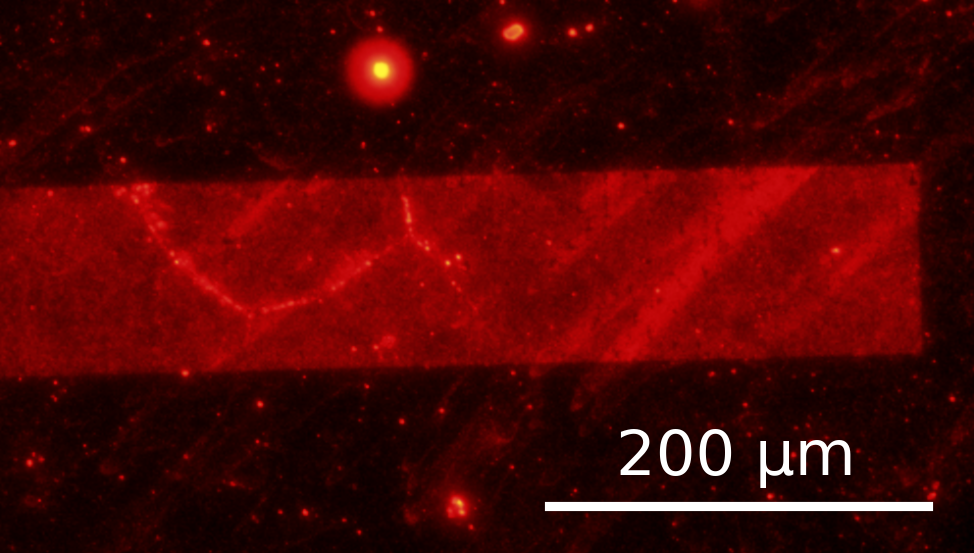
\includegraphics[width=0.5\textwidth,height=\textheight]{figures/ch2/modified_NGW8D4_1mM_rhodamineB_centralchannel3_postMsurfactantclean5min_2.4sexposure_20X_221111.png}

}

\caption[Fluorescence image of a strip of graphene functionalised with
Rhodamine B dye with graphene folds
visible.]{\label{fig-graphene-folds}Fluorescence image of a strip of
graphene on SiO\(_2\) surface functionalised with Rhodamine B dye.
Bright lines are visible on the left side of the graphene surface which
correspond to preferential attachment of dye along the graphene folds.}

\end{figure}

There are multiple methods for depositing graphene onto a wafer for
subsequent device fabrication, including mechanical exfoliation,
epitaxial growth and chemical vapour deposition (CVD)
\autocite{Reddy2011}. While the CVD process is relatively simple and
cheap, the initial deposition of graphene onto copper often leads to the
creation of folds (or wrinkles) of up to \(\sim\) 6 nanometers in height
across the surface of a graphene monolayer \autocite{Zhu2012}. This
occurs as a result of the rapid cooling process that takes place after
deposition, where copper thermally contracts more than graphene. Since
the graphene is pinned to the surface, this leads to slight folding of
the monolayer \autocite{Zhao2012,Zhu2012,Chhikara2013}. Transferring
graphene from the rough copper to a relatively smooth Si/SiO\(_2\) wafer
can also contribute to wrinkling \autocite{Zhao2012,Kireev2017}. These
folds help to mechanically stabilise the graphene layer, but have
significant negative effects on charge transport
\autocite{Geim2007,Chhikara2013,Zhu2012}. Folds also exhibit enhanced
reactivity due to their low radius of curvature \autocite{Zhao2012}.
This is demonstrated in Figure~\ref{fig-graphene-folds}, where the
fluorescent Rhodamine B dye preferentially bonds to folded regions,
leading to particularly dense functionalisation in these regions. This
behaviour has previously been observed for the decoration of graphene
with pentacene molecules \autocite{Chhikara2013}. Other defects
influencing surface reactivity include grain boundaries and point
defects in the crystal structure
\autocite{Zhao2012,Chhikara2013,Kireev2017}.

\hypertarget{sec-electrical-characterisation-graphene}{%
\subsection{Electrical
Characterisation}\label{sec-electrical-characterisation-graphene}}

The transfer sweep behaviour of a graphene device is ambipolar and has
no off regime under standard conditions
\autocite{Novoselov2004,Bartolomeo2011,Ohno2015}. When a gate voltage
\(V_g\) is applied to the channel of a graphene device, the Fermi energy
of the graphene is shifted and surface charge density is altered
\autocite{Novoselov2004,Heller2010,Ohno2015}. An increase in surface
charge density means an increase in carriers available for either \(p\)
or \(n\)-conduction and increased \(I_d\) \autocite{Geim2007}. The
regions of hole conduction and electron conduction are shown in
Figure~\ref{fig-graphene-characteristics} (a), alongside the
corresponding Fermi energy on the simplified graphene bandstructure
(known as a ``Dirac cone'') \autocite{Geim2007,Ohno2015}. The
transconductance of the curve at \(V_g\) = 0 V, \(g_m\) = 1 µS, is
similar to the liquid-gated transconductance of a carbon nanotube device
shown earlier. As graphene lacks a bandgap, there is a minimum possible
conductance for graphene devices, which leads to a relatively small
on-off ratio \autocite{Novoselov2004,Geim2007}. Folding may further
decrease on-off ratio due to diffusive transport of carriers along the
folds \autocite{Zhu2012}. The on-off ratio of the graphene transfer
curve shown in Figure~\ref{fig-graphene-characteristics} (a) is 5. A
bandgap can be introduced to a graphene device using a dual-gated
configuration, where both back-gate and top-gate can be swept
simultaneously, increasing the on-off ratio past 100
\autocite{Xia2010,Ahn2020,Shkodra2021}.

\begin{figure}

\begin{minipage}[t]{0.03\linewidth}

{\centering 

\raisebox{-\height}{


\includegraphics{figures/(a).png}

}

}

\end{minipage}%
%
\begin{minipage}[t]{0.01\linewidth}

{\centering 

~

}

\end{minipage}%
%
\begin{minipage}[t]{0.45\linewidth}

{\centering 

\raisebox{-\height}{

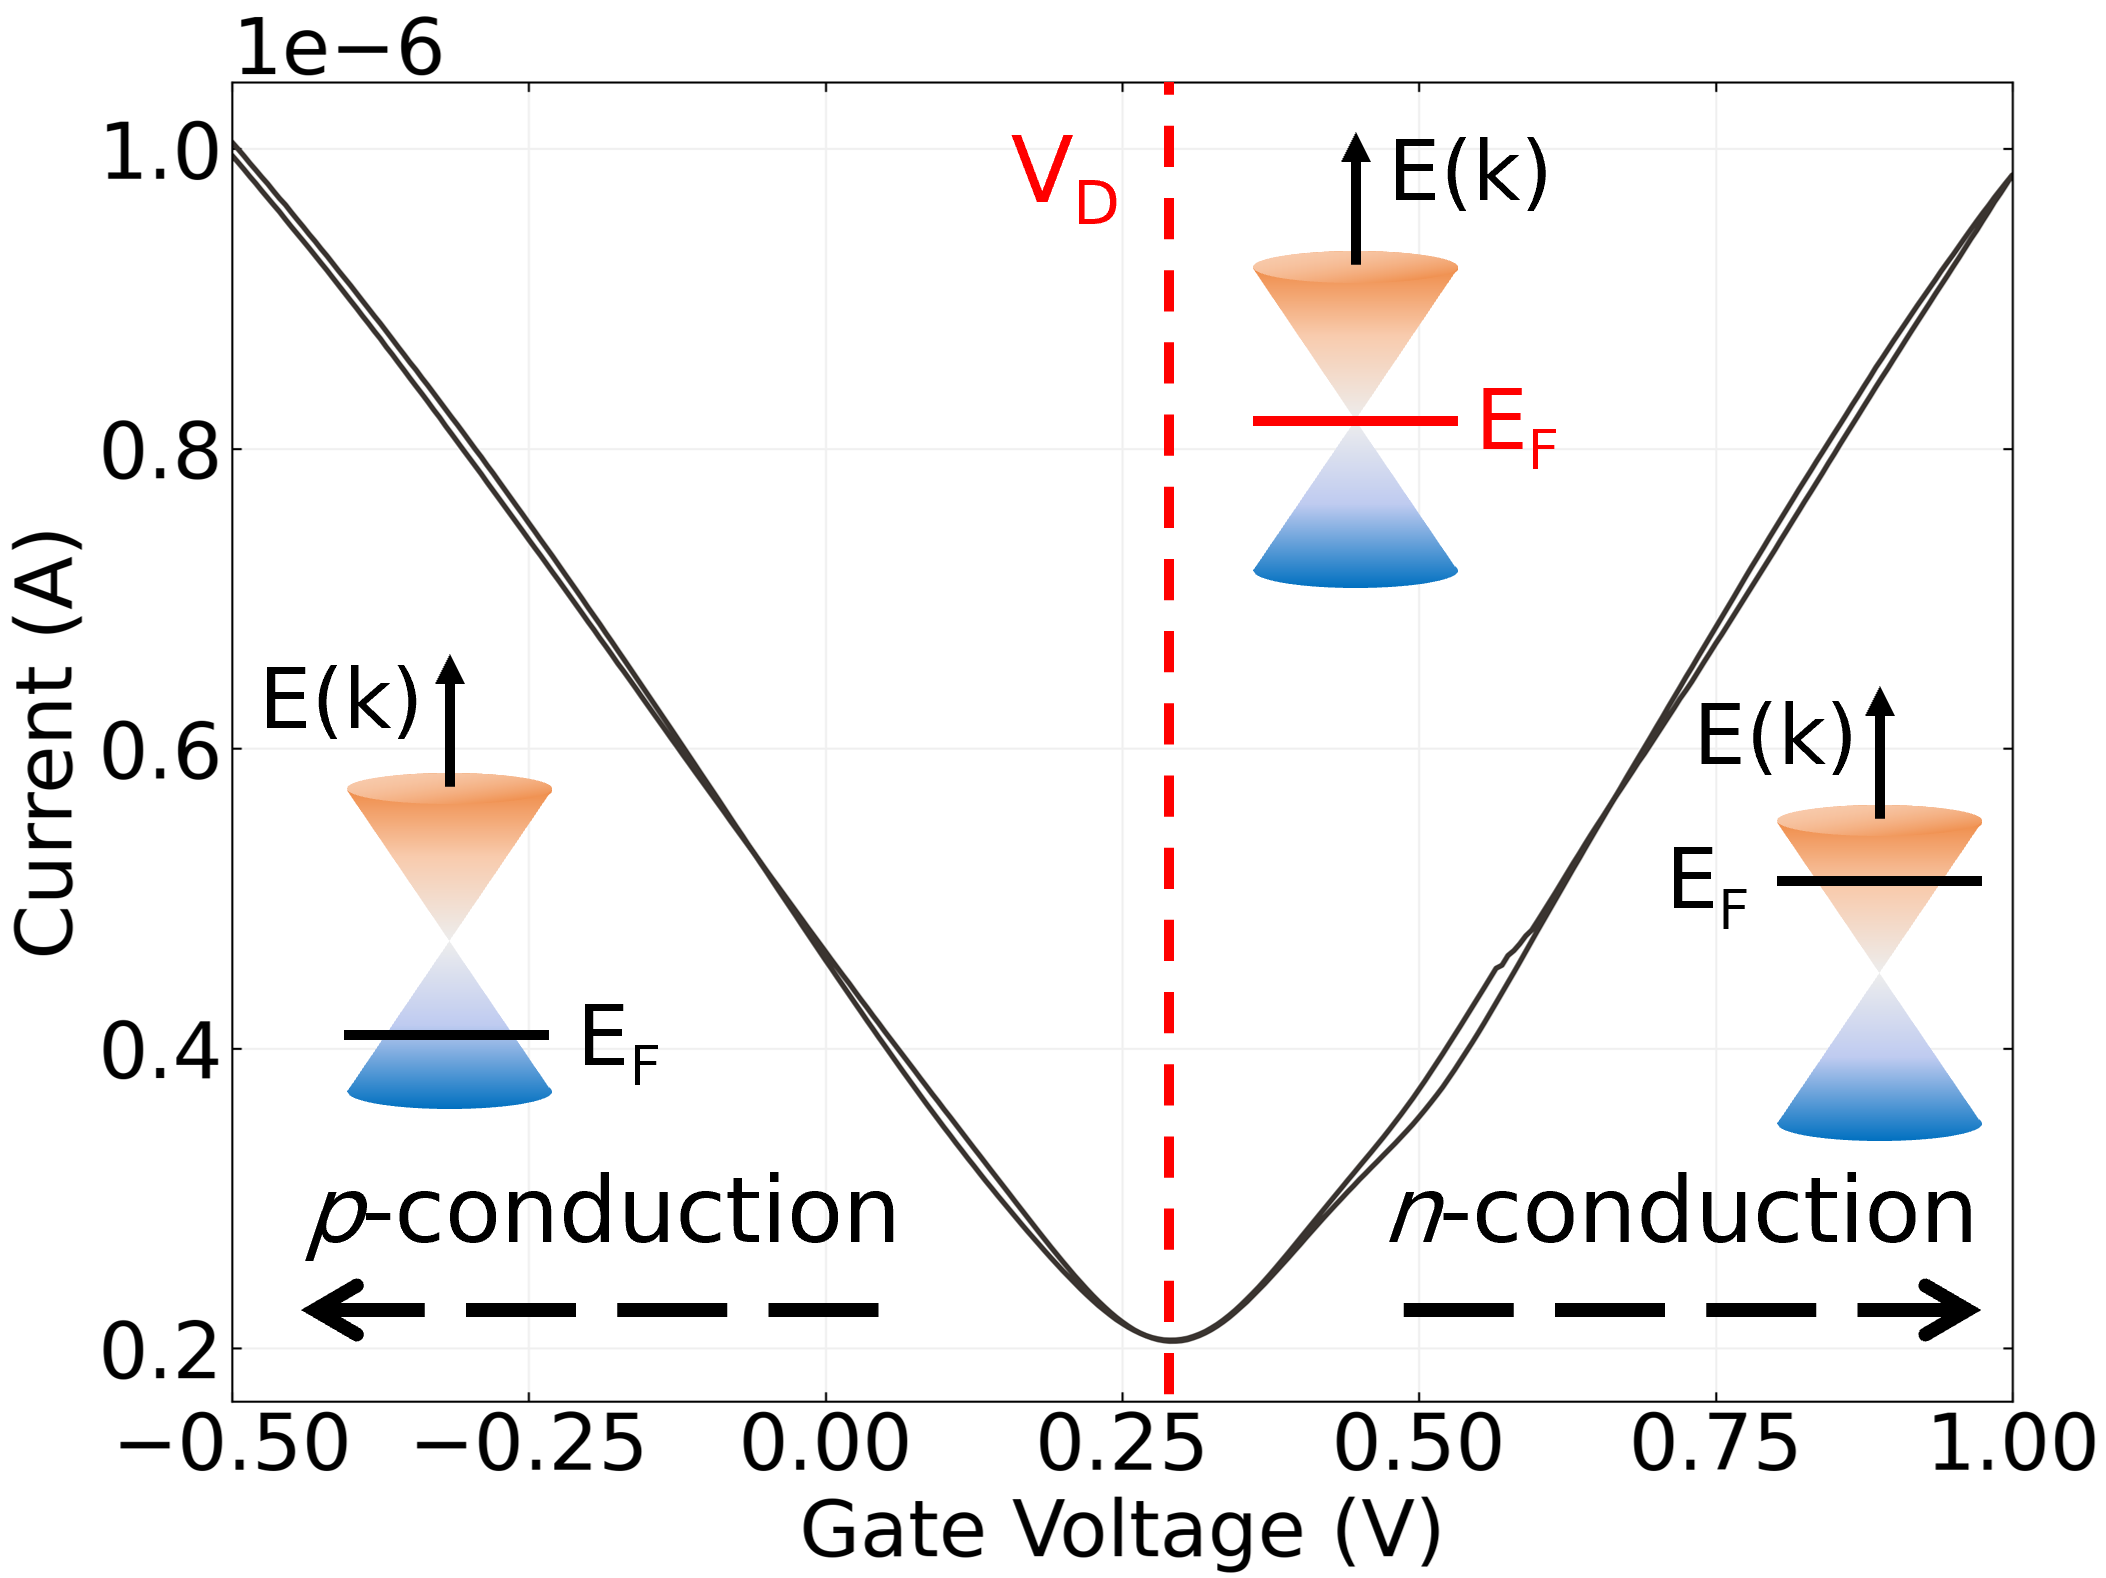
\includegraphics{figures/ch2/Graphene_transfer_1.png}

}

}

\end{minipage}%
%
\begin{minipage}[t]{0.01\linewidth}

{\centering 

~

}

\end{minipage}%
%
\begin{minipage}[t]{0.03\linewidth}

{\centering 

\raisebox{-\height}{


\includegraphics{figures/(b).png}

}

}

\end{minipage}%
%
\begin{minipage}[t]{0.01\linewidth}

{\centering 

~

}

\end{minipage}%
%
\begin{minipage}[t]{0.45\linewidth}

{\centering 

\raisebox{-\height}{

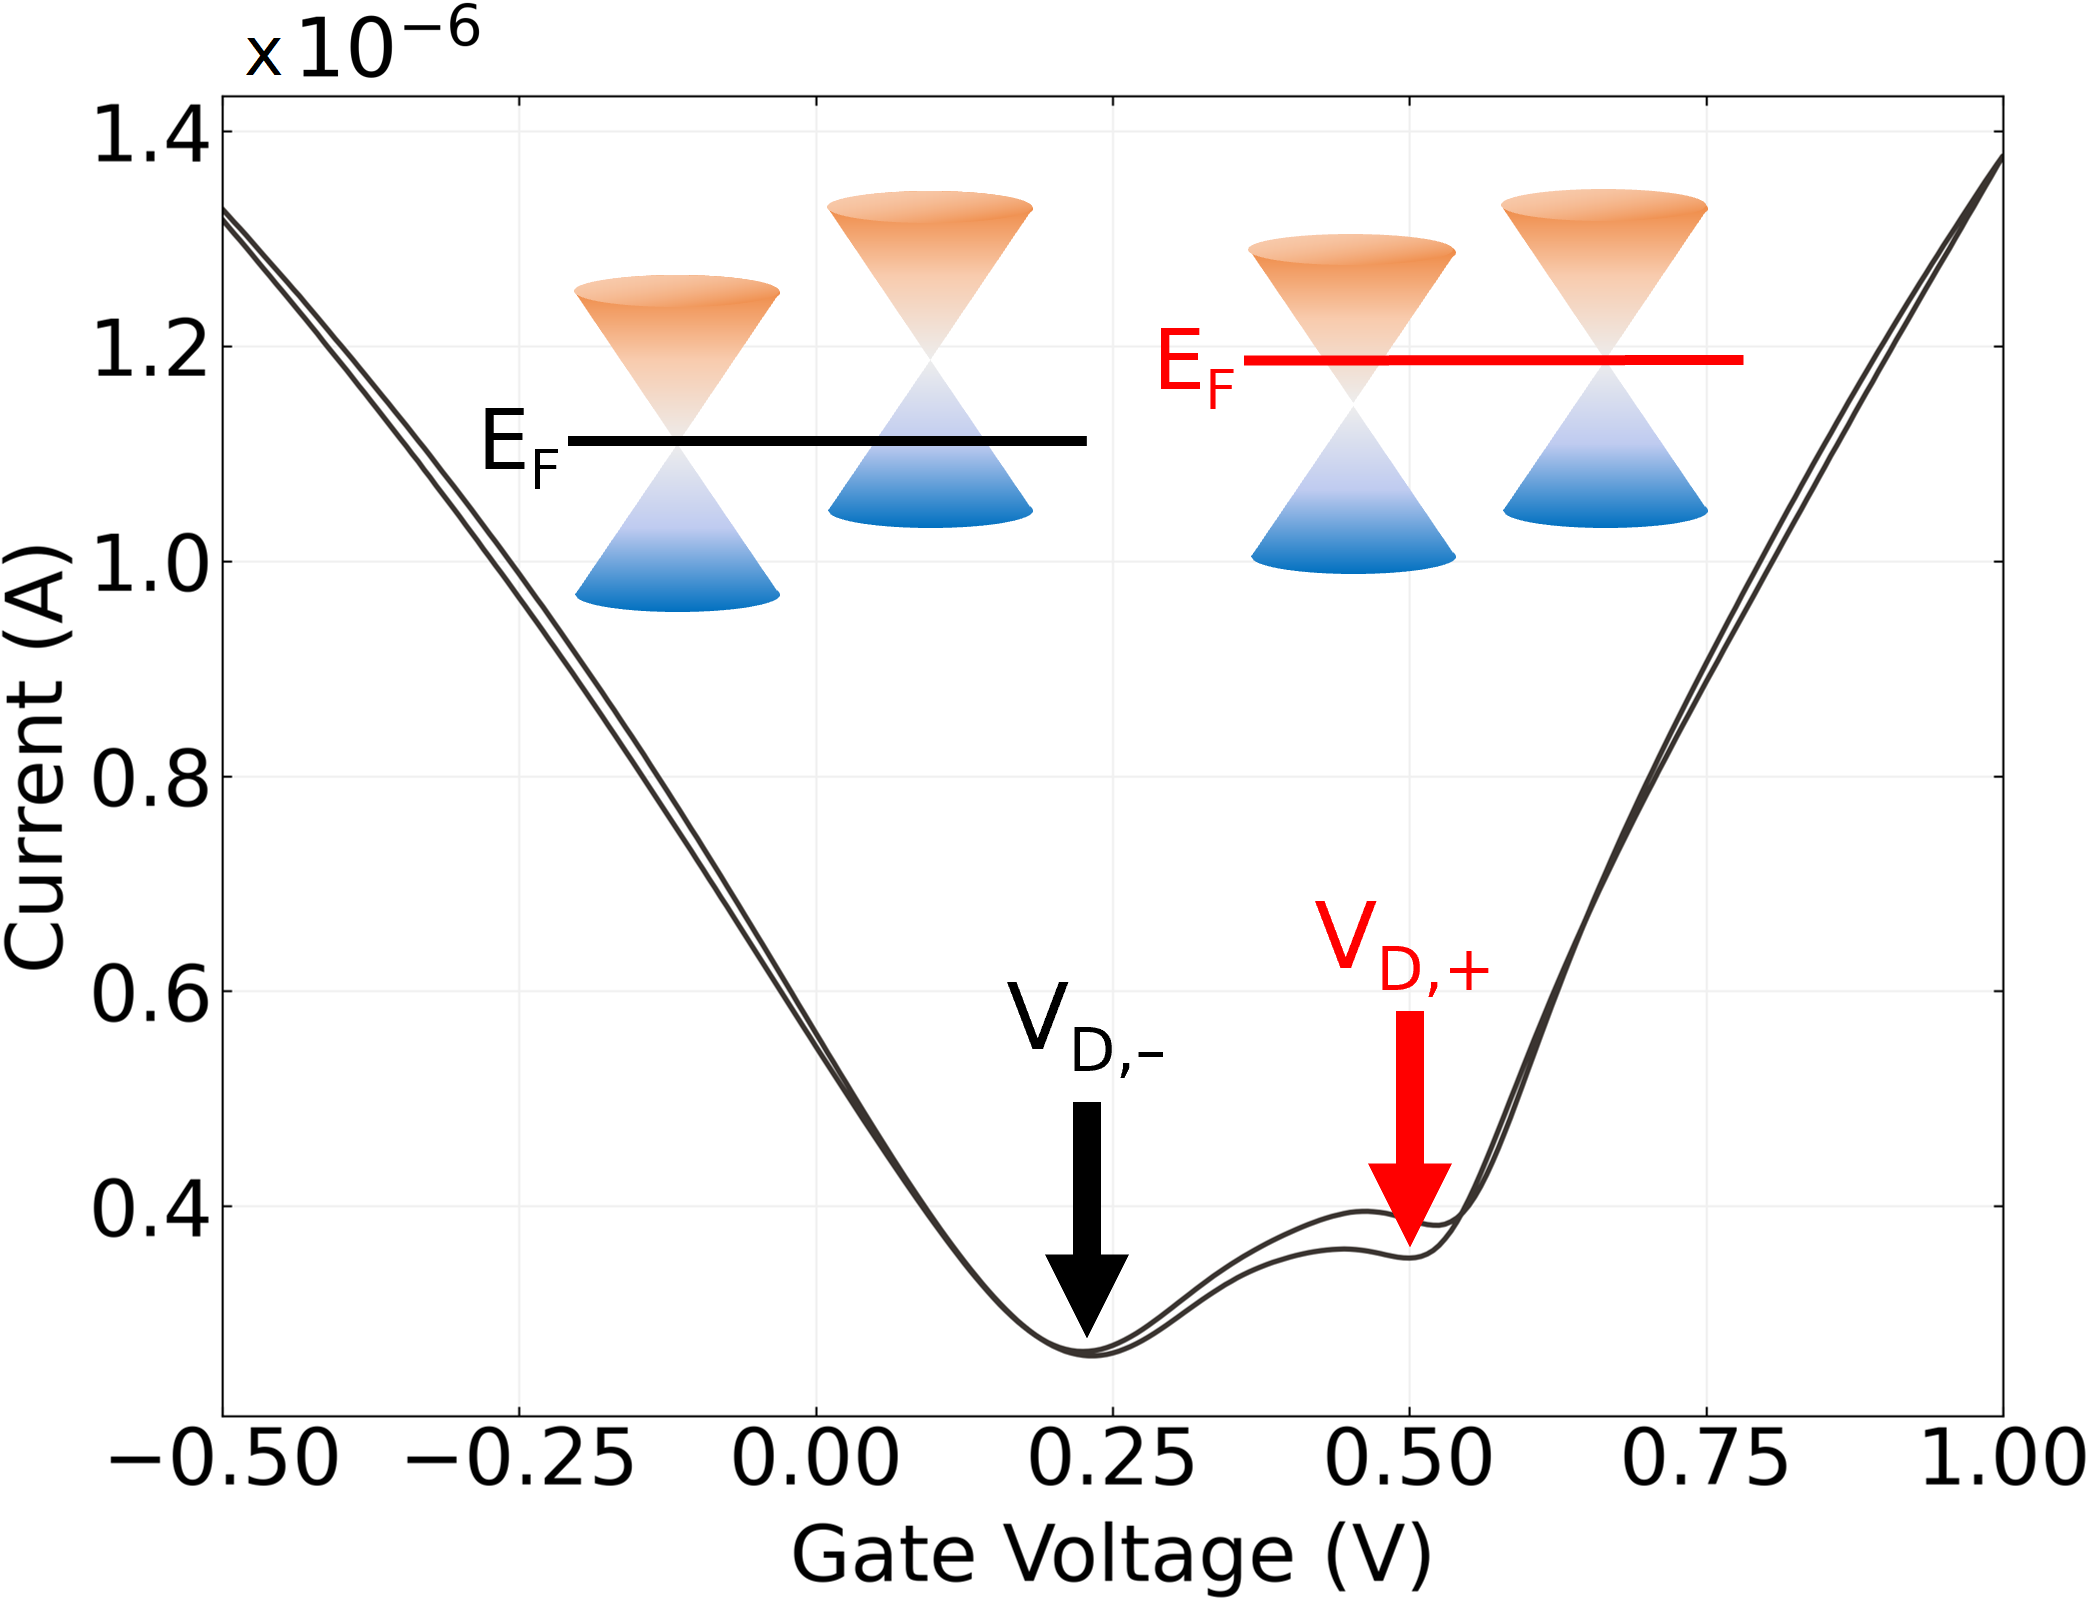
\includegraphics{figures/ch2/Graphene_transfer_2.png}

}

}

\end{minipage}%
%
\begin{minipage}[t]{0.01\linewidth}

{\centering 

~

}

\end{minipage}%

\caption[Liquid-gated transfer characteristics of two graphene
field-effect transistor channels, one of which exhibits a double-minimum
feature seen in longer transistor
channels.]{\label{fig-graphene-characteristics}Liquid-gated transfer
characteristics of two graphene field-effect transistor channels, one of
which exhibits a double-minimum feature seen in longer transistor
channels. In (a), the Dirac point voltage is indicated by a red line,
and regions of hole conduction and electron conduction are also shown.
The relative Fermi energy in each region is shown on simplified graphene
bandstructure insets. The graphene channel in (b) has double conduction
minima, which are highlighted with red arrows. The relative Fermi energy
at each minima is also shown on bandstructure insets.}

\end{figure}

The minimum conductance obtainable by gating in a graphene device occurs
at what is known as the charge neutrality or Dirac point, where the
population of charge carriers is at a minimum
\autocite{Novoselov2004,Bartolomeo2011,Ohno2015,Kireev2017}. At gate
voltages close to the Dirac voltage, both electrons and holes are
present, and at the Dirac point, there are equal concentrations of each
carrier present \autocite{Novoselov2004,Bartolomeo2011,Peng2018}. As
shown in Figure~\ref{fig-graphene-characteristics} (a), as the gate
voltage moves left away from the Dirac voltage and Fermi energy is
shifted into the valence band, holes begin to dominate conduction, while
as gate voltage is moved to the right of the Dirac voltage, where Fermi
energy is shifted into the conduction band, electrons dominate
\autocite{Novoselov2004,Bartolomeo2011,Feng2014,Zhang2015}. At points
far from the Dirac voltage, conductivity increases linearly
\autocite{Novoselov2004,Bartolomeo2011,Peng2018}. Typically, a monolayer
graphene channel conducts holes at zero gate voltage, which results from
the presence of \(p\)-dopants such as oxygen and water adsorbed from the
air and resist residues. By removing these dopants, the Dirac point
feature can be brought closer to the zero gate voltage position on the
transfer curve, indicating graphene is naturally a mixed-carrier
conductor
\autocite{Novoselov2004,Bartolomeo2011,Zhang2015,Kireev2017,Peng2018}.

Some graphene devices naturally exhibit a double-minimum feature in the
transfer characteristic curve, corresponding to two separate Dirac
points \autocite{Bartolomeo2011,Feng2014,Zhang2015,Kireev2017,Peng2018}.
This effect is due to doping of graphene by charge transfer from the
metal contacts. In shorter length channels, metal doping affects the
entire channel length. Band bending from channel doping near the metal
contact results in a consistent Fermi level across the channel, meaning
only a single Dirac point is present in the transfer characteristic
curve. However, for longer channels, metal doping no longer occurs
across the entire channel length \autocite{Bartolomeo2011,Peng2018}.
This discrepancy leads to a difference in Fermi level between the
metal-doped graphene and graphene in the unaffected channel region
\autocite{Bartolomeo2011,Feng2014,Peng2018,Zhang2015}. The difference in
Fermi levels results in the introduction of a second Dirac point. The
relative level of doping in the metal-doped and unaffected channel
regions determines the relative \(V_g\) position of each local minimum
on the \(I_d - V_g\) curve \autocite{Bartolomeo2011,Peng2018,Zhang2015}.

Figure~\ref{fig-graphene-characteristics} (b) shows a double-minimum
transfer characteristic with each Dirac point indicated
\autocite{Peng2018}. At large negative \(V_g\), the Fermi energy level
is far from the Dirac point energy of both the channel and contact
regions, and holes dominate conduction. As \(V_g\) and the Fermi energy
approach and then pass the Dirac point corresponding to the left minimum
\(V_{D,-}\), the available carriers decrease to a minimum and begin to
increase again in one region \(R_1\), but continuously decrease in the
other region \(R_2\). The shape of the curve between \(V_{D,-}\) and the
right local minimum \(V_{D,+}\) then depends on the relative rate of
increasing electron and decreasing hole populations, where the graphene
is \(n\)-doped in \(R_1\) and \(p\)-doped in \(R_2\). At the local
minimum on the right, \(V_{D,+}\), the carriers in \(R_2\) now reach a
minimum, while carriers in \(R_1\) continue to increase. At voltages
well beyond \(V_{D,+}\), electrons then dominate conduction in both
regions \autocite{Bartolomeo2011,Zhang2015,Peng2018}.

\hypertarget{sensing-behaviour}{%
\subsection{Sensing Behaviour}\label{sensing-behaviour}}

The large surface-to-volume ratio of graphene makes it highly sensitive
to intermolecular interactions and therefore appropriate for use in
sensing applications \autocite{Ohno2015,Tran2016}. An analyte molecule
can be detected using a graphene channel by observing the change in
current that occurs when the presence of a charged analyte alters the
channel Fermi level \autocite{Heller2010,Ohno2015}. Sensing may be
dominated by interactions occurring at the graphene folds
\autocite{Zhao2012}. The small on-off ratio of graphene is a drawback
when used in field-effect transistor sensing applications when compared
with carbon nanotube transistors \autocite{Novoselov2004}. If a
dual-gate configuration is used, however, on-off ratio can be increased
significantly by introducing a bandgap. The presence of a bandgap means
a Schottky barrier is introduced at the graphene-electrode interface,
whose modulation can then also contribute as a potential sensing
mechanism (see Section~\ref{sec-cnt-network-details} for a discussion of
Schottky barriers) \autocite{Xia2010}.

\hypertarget{carbon-nanotube-field-effect-transistors}{%
\section{Carbon Nanotube Field-Effect
Transistors}\label{carbon-nanotube-field-effect-transistors}}

\hypertarget{sec-carbon-nanotubes}{%
\subsection{Carbon Nanotube Properties}\label{sec-carbon-nanotubes}}

\begin{figure}

{\centering 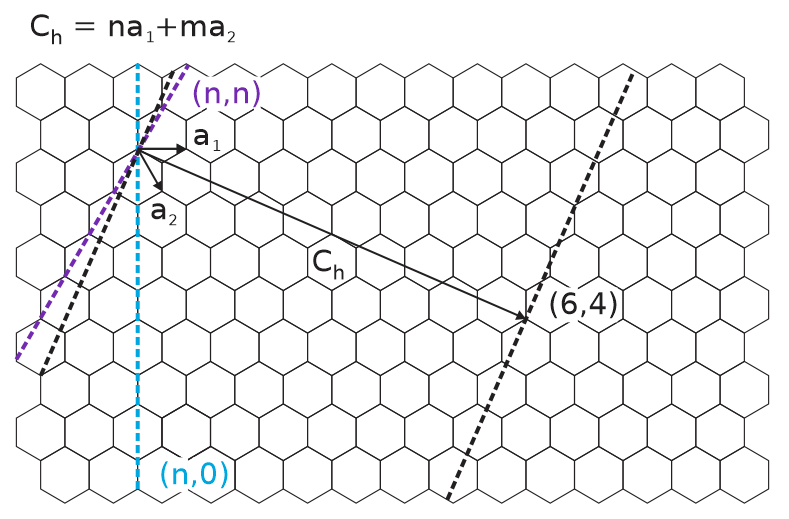
\includegraphics[width=0.6\textwidth,height=\textheight]{figures/ch2/carbon_nanotube_wrapping.png}

}

\caption[Diagram illustrating how a graphene sheet can be rolled up at
various angles to form carbon
nanotubes.]{\label{fig-carbon-nanotube-wrapping}Diagram illustrating how
a graphene sheet can be rolled up at various angles to form carbon
nanotubes. The two black dotted lines represent boundaries which can be
cut across and then brought into contact to form a cylinder. The
cylinder here is referred to by the integer pair (6,4), since the chiral
vector \(C_h\), the vector perpendicular to the cut through the sheet,
is given by \(C_h = 6a_1+4a_2\). The chiral vector forms the
circumference of the rolled carbon nanotube. The left edge in the zigzag
(\(n\),0) and armchair (\(n\),\(n\)) cases are shown with a blue and
purple dotted line respectively. The location of the right edge
(diameter of the nanotube) is determined by the value chosen for \(n\).}

\end{figure}

Since their initial identification in 1991 \autocite{Iijima1991}, a wide
range of applications for carbon nanotubes (CNTs) have been proposed,
due to their small mass, elasticity, strength, and unique electronic
properties. A single-walled carbon nanotube (SWCNT) consists of a
monolayer graphene sheet rolled up into a cylinder, while a multi-walled
carbon nanotube (MWCNT) consists of several monolayer graphene cylinders
where smaller cylinders are coaxially contained by larger cylinders
\autocite{Dekker1999,Avouris2007,Cao2009,Rouhi2010,Shkodra2021}.
Multi-walled carbon nanotubes can suffer from significant scattering at
defects leading to diffusive electron motion \autocite{Dekker1999}.
However, single-walled carbon nanotubes are relatively defect-free, and
carrier transport within nanotubes is near-ballistic at room
temperature, resulting in high carrier mobility
\autocite{Dekker1999,Avouris2007,Cao2009,Rouhi2010,Shkodra2021}. The
momentum of charge carriers in a single-walled carbon nanotube is
quantised, confining carriers to 2-dimensional slices across the
3-dimensional graphene bandstructure. If a slice contains a bandgap, the
carbon nanotube behaves as a semiconductor (s-CNT); if not, the nanotube
behaves as a metal (m-CNT) \autocite{McEuen2002}. The high
surface-to-volume ratio of small-diameter single-walled carbon nanotubes
makes them extremely sensitive and therefore particularly suitable for
sensing applications \autocite{Cao2009,Yao2021,Shkodra2021}. Like
graphene, carbon nanotubes have a large potential window, and can be
used safely in a liquid-gate environment without undergoing redox
reactions \autocite{Ohno2015}.

The chirality and diameter of a carbon nanotube determines its
electronic bandstructure and whether it has semiconducting or metallic
characteristics
\autocite{Martel1998,Dekker1999,McEuen2002,Avouris2007,Shkodra2021,Li2023}.
The chirality indices of a nanotube (\(n, m\)) determines the chiral
angle at which hexagons wind around the nanotube relative to the
longitudinal axis of the nanotube. This chiral angle is the angle
between the chiral vector
\(\textbf{C}_h = n\textbf{a}_1+m\textbf{a}_2\), which maps to the
circumference of the nanotube, and the basis vector \(\textbf{a}_1\),
which is parallel to a row of hexagons. The size of the chiral angle
\(\theta\) is given by Equation~\ref{eq-chiral-angle}, and the diameter
of the resulting carbon nanotube is given by \(d=|C_h|/\pi\)
\autocite{Lu2012}.

\begin{equation}\protect\hypertarget{eq-chiral-angle}{}{
\theta = \arcsin\frac{\sqrt{3}m}{2\sqrt{n^2+nm+m^2}}, \space n > m
}\label{eq-chiral-angle}\end{equation}

When \(m= 0\), \(\theta = 0°\), and the resulting carbon nanotube has a
``zigzag'' structure; when \(m = n\), \(\theta = 30°\), and the carbon
nanotube has an ``armchair'' structure. When \(\theta\) is between
\(0°-30°\), the structure is referred to as ``chiral''
\autocite{Dekker1999,Lu2012}. When \(n-m = 3z\), where \(z\) is an
integer, the resulting carbon nanotube is metallic \(-\) for example, if
\(n=5\) and \(m=5\), \(z=0\), therefore the tube is metallic. All other
nanotubes are semiconducting, including the (6, 4) chiral nanotube
described in Figure~\ref{fig-carbon-nanotube-wrapping}. Out of the
chiral arrangements available, two-thirds of the possible structures are
semiconducting while one-third is metallic \autocite{Dekker1999}.

\hypertarget{sec-cnt-network-details}{%
\subsection{Carbon Nanotube Network
Transistors}\label{sec-cnt-network-details}}

The first carbon nanotube transistors were created in 1998, and used a
single carbon nanotube as the device channel
\autocite{Martel1998,Tans1998,Kauffman2008}. Over the following decade,
there was a general move away from the use of a single tube as the
transistor channel towards that of a large-scale network of carbon
nanotubes. In these networks, the individual electrical properties of
the CNTs are averaged out across the network, reducing device-to-device
variation. Furthermore, the large area of coverage ensures high channel
mobility. The network morphology is therefore generally preferred in
sensing applications \autocite{Hu2004,Cao2009,Murugathas2019,Li2023}.
The carbon nanotube network used for the channel can either be
directionally-aligned or randomly deposited
\autocite{Cao2009,Shkodra2021}; in this thesis, randomly deposited
networks were fabricated using facile solution-deposition methods
\autocite{Zheng2017,Cassie2023}. Important attributes of a carbon
nanotube film include the density of the network (number of nanotubes
per unit area), the ratio of metallic to semiconducting nanotubes
present, and the distribution of nanotube diameters present
\autocite{Cao2009,Shkodra2021}. The strong van der Waals forces between
carbon nanotubes lead to them bundling together within a network. These
bundles may contain many nanotubes of different size and chirality
\autocite{Fuhrer2000,Hu2004,Cao2009,Murugathas2019}.

The band bending which occurs at the interface between the metal
electrodes of the device and the semiconducting carbon nanotubes is
primarily responsible for carbon nanotube field-effect transistor
switching behaviour \autocite{Avouris2007,Bargaoui2018}. The Fermi level
difference between materials leads to free electrons flowing across each
interface until the Fermi levels equilibrate and a electric dipole layer
forms. The net electric field created at each interface creates a space
charge region in the channel, resulting in a potential step known as a
``Schottky barrier''. The net electric field also results in curvature
of the bandstructure at the metal-semiconductor interface, which is why
this process is referred to as ``band bending'' \autocite{Zhang2012}.
Current primarily flows through the semiconductor channel by
quantum-mechanically tunnelling through the Schottky barriers present at
each electrode. The width of the Schottky barriers can be modulated by
changing the gate voltage of the device, which can increase or decrease
current flow across the channel depending on the magnitude and polarity
of the gate voltage \autocite{Avouris2007,Bargaoui2018}. As CNT FETs are
ambipolar, it is possible for both holes and electrons to flow across
the channel; highly negative gate voltages lead to hole conduction while
positive voltages lead to electron conduction \autocite{Avouris2007}.

\begin{figure}

\begin{minipage}[t]{0.03\linewidth}

{\centering 

\raisebox{-\height}{


\includegraphics{figures/(a).png}

}

}

\end{minipage}%
%
\begin{minipage}[t]{0.01\linewidth}

{\centering 

~

}

\end{minipage}%
%
\begin{minipage}[t]{0.45\linewidth}

{\centering 

\raisebox{-\height}{

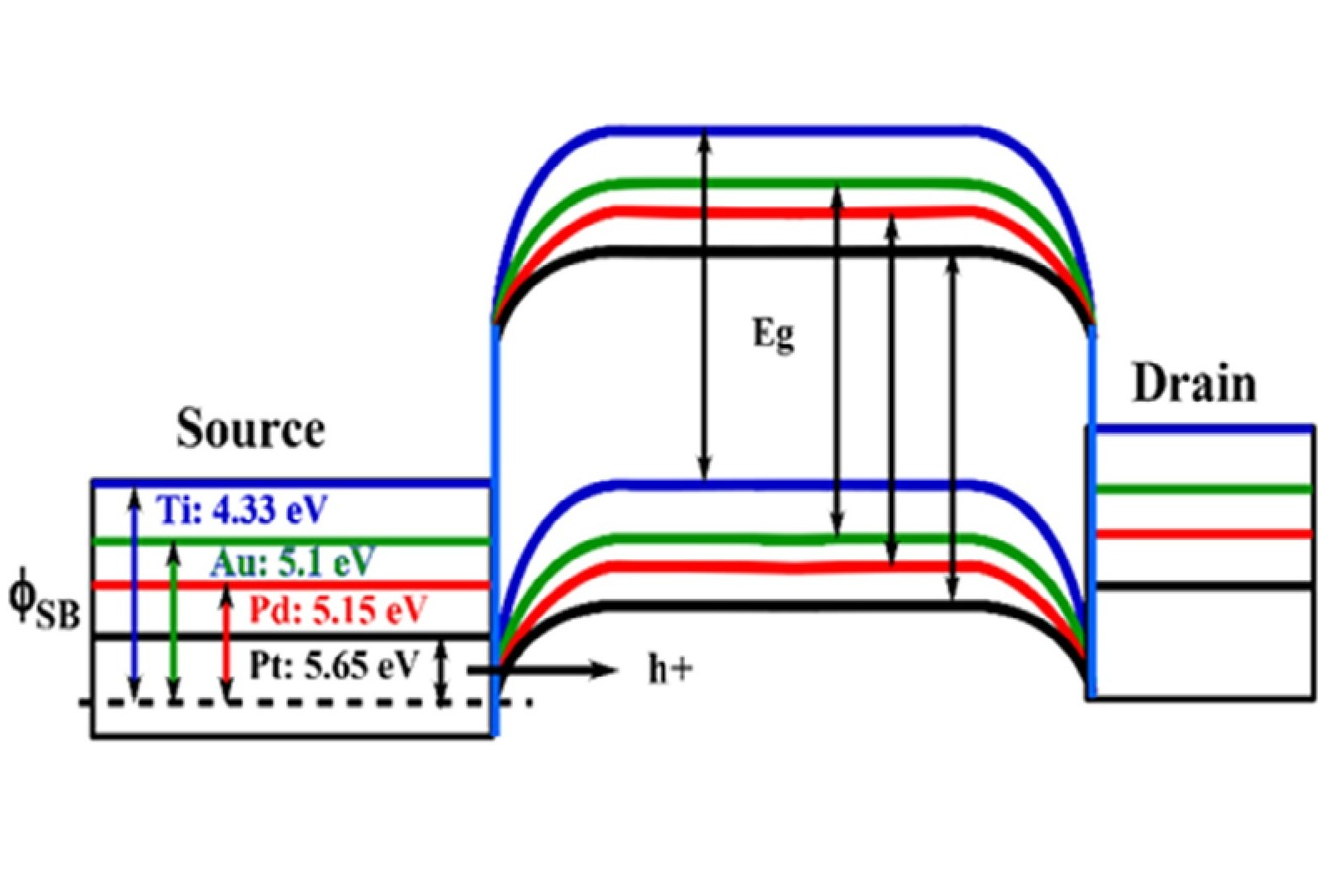
\includegraphics{figures/ch2/band-bending.png}

}

}

\end{minipage}%
%
\begin{minipage}[t]{0.01\linewidth}

{\centering 

~

}

\end{minipage}%
%
\begin{minipage}[t]{0.03\linewidth}

{\centering 

\raisebox{-\height}{


\includegraphics{figures/(b).png}

}

}

\end{minipage}%
%
\begin{minipage}[t]{0.01\linewidth}

{\centering 

~

}

\end{minipage}%
%
\begin{minipage}[t]{0.45\linewidth}

{\centering 

\raisebox{-\height}{

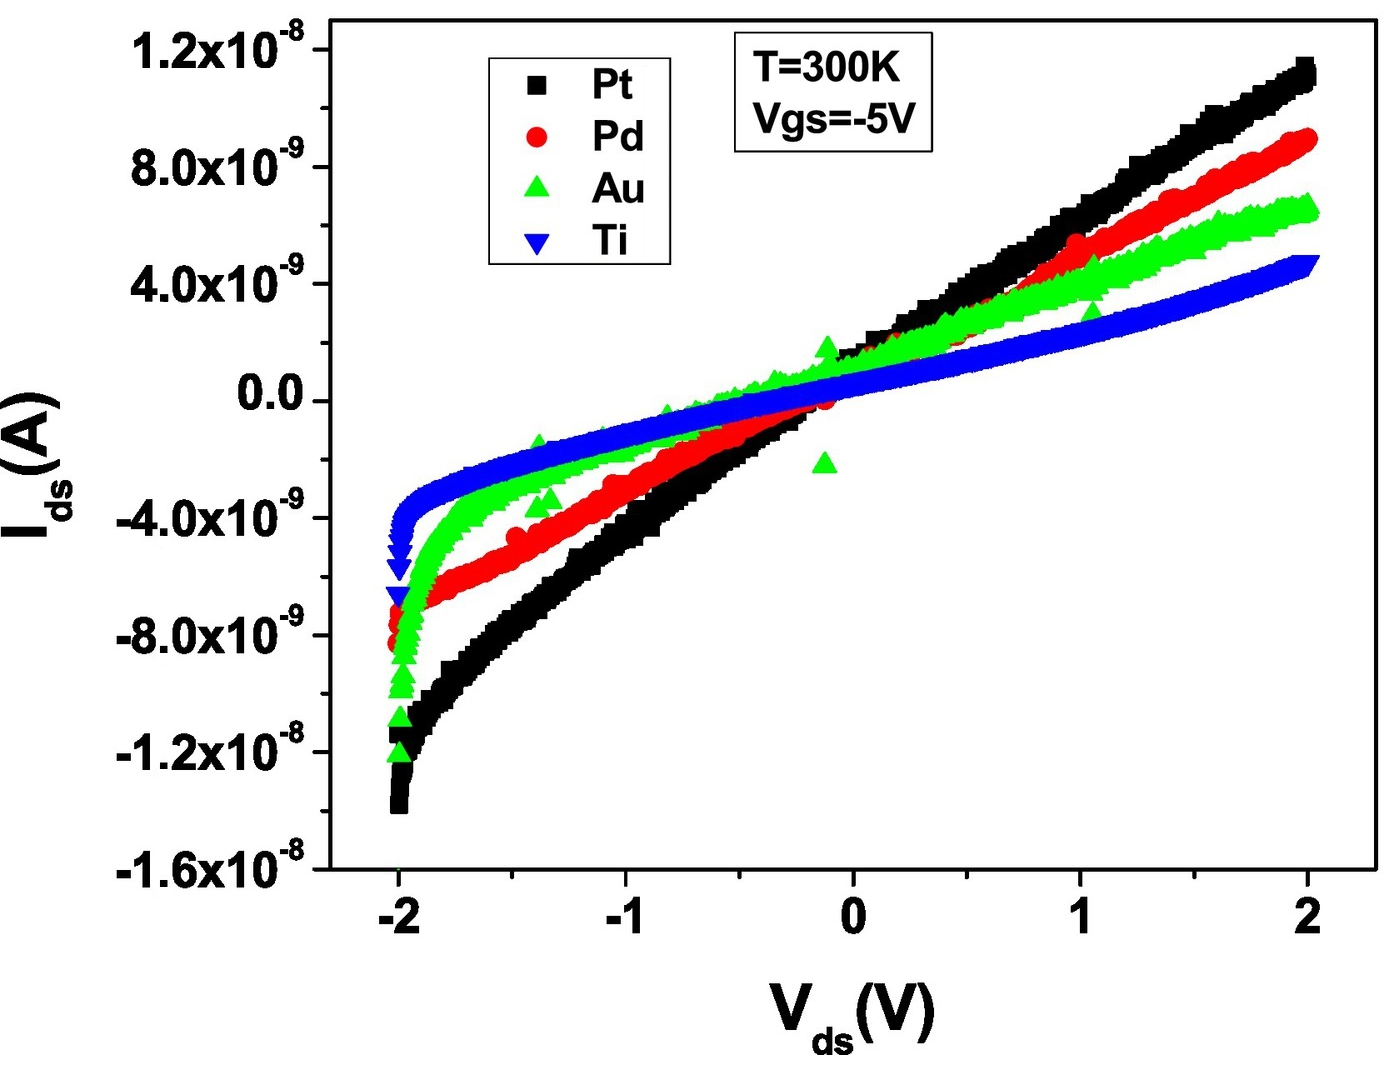
\includegraphics{figures/ch2/band-bending-current.png}

}

}

\end{minipage}%
%
\begin{minipage}[t]{0.01\linewidth}

{\centering 

~

}

\end{minipage}%

\caption[Figure which shows the band bending occurring at the metal-CNT
network interface with corresponding output characteristic
curves.]{\label{fig-band-bending}The band bending which occurs at the
metal-CNT network interface is shown in (a) for platinum, palladium,
gold and titanium electrodes, where \(\phi_{SB}\) is Schottky barrier
height and \(E_g\) is bandgap size. The output characteristic curves of
devices with these electrodes are shown in (b), where the devices are
gated fully on at \(V_g = -5\) V. Reproduced with permission from
\autocite{Bargaoui2018}. Copyright \(\copyright\) 2018 Elsevier.}

\end{figure}

The relative height of the Schottky barriers present at the electrical
contacts influences the magnitude of on-current obtainable by a device.
An important factor in determining the Schottky barrier height of a
device is the type of metal used for the contact, with the relationship
between the type of metal used and resulting device on-current shown in
Figure~\ref{fig-band-bending}. Titanium has a relatively low work
function of 4.3 eV, leading to larger Schottky barriers at the
electrodes and relatively low device on-current, while platinum has a
relatively high work function of 5.7 eV, leading to smaller Schottky
barriers and relatively high device on-current \autocite{Bargaoui2018}.
The Schottky barrier height also influences the size of hole on-current
relative to electron on-current. A high work function metal like
palladium bends the valence band of the semiconductor towards the Fermi
level of the metal, creating a low barrier for holes but a high barrier
for electrons, leading to a much higher hole on-current as compared to
electron on-current. A low work function metal like aluminium, on the
other hand, has a relatively low work function, giving rise to a larger
on-current for electrons and smaller on-current for holes
\autocite{Chen2005,Avouris2007,Bargaoui2018}.

\begin{figure}

\begin{minipage}[t]{0.03\linewidth}

{\centering 

\raisebox{-\height}{


\includegraphics{figures/(a).png}

}

}

\end{minipage}%
%
\begin{minipage}[t]{0.01\linewidth}

{\centering 

~

}

\end{minipage}%
%
\begin{minipage}[t]{0.50\linewidth}

{\centering 

\raisebox{-\height}{

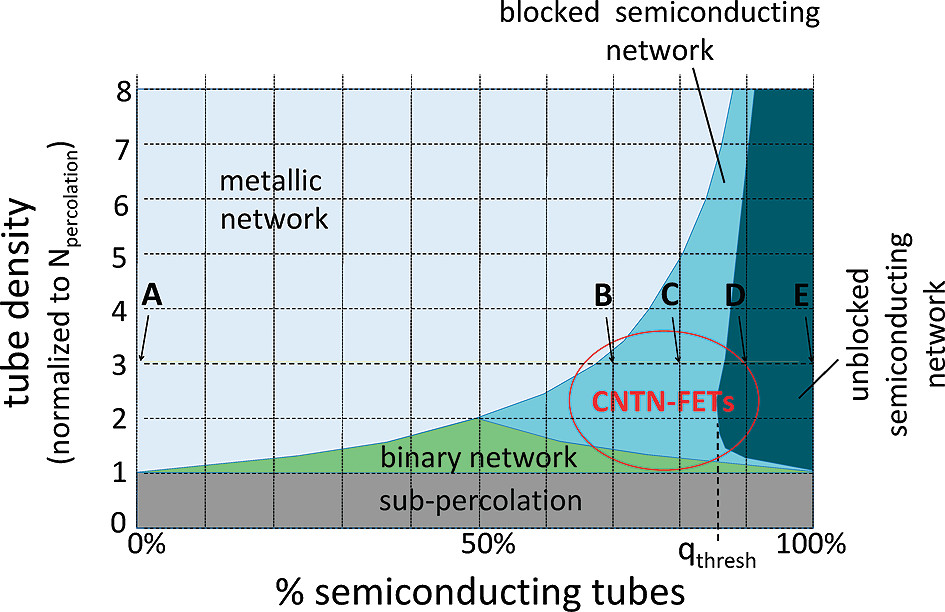
\includegraphics{figures/ch2/semiconducting-proportion-density.png}

}

}

\end{minipage}%
%
\begin{minipage}[t]{0.01\linewidth}

{\centering 

~

}

\end{minipage}%
%
\begin{minipage}[t]{0.03\linewidth}

{\centering 

\raisebox{-\height}{


\includegraphics{figures/(b).png}

}

}

\end{minipage}%
%
\begin{minipage}[t]{0.01\linewidth}

{\centering 

~

}

\end{minipage}%
%
\begin{minipage}[t]{0.40\linewidth}

{\centering 

\raisebox{-\height}{

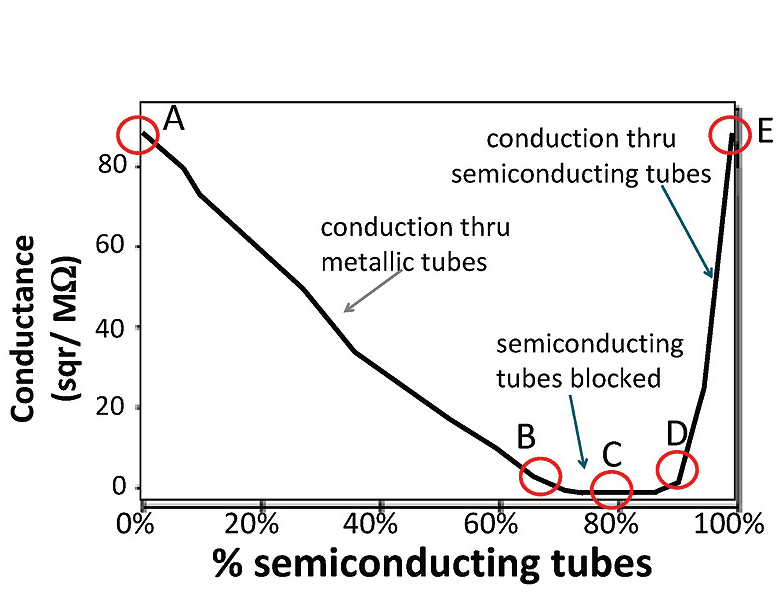
\includegraphics{figures/ch2/semiconducting-proportion.png}

}

}

\end{minipage}%
%
\begin{minipage}[t]{0.01\linewidth}

{\centering 

~

}

\end{minipage}%

\caption[Figures showing the relationship between the proportion of
semiconducting tubes present, the network density relative to the
percolation threshold, and the general electronic behaviour of the
resulting carbon nanotube network.]{\label{fig-m-s-junctions}The phase
diagram in (a) shows the relationship between the proportion of
semiconducting tubes present, the network density relative to the
percolation threshold, and the general electronic behaviour of the
resulting carbon nanotube network. The relationship between network
conductance and proportion of semiconducting tubes present is shown in
(b), in the specific case where density was roughly 3 times the
percolation threshold (in the case where all tubes were either metallic
or semiconducting). Specific morphologies A, B, C, D and E are shown on
both figures. Reprinted with permission from \autocite{Topinka2009}.
Copyright \(\copyright\) 2009 American Chemical Society.}

\end{figure}

The behaviour of carbon nanotube network transistors is also influenced
by a variety of potential barriers existing at junctions between carbon
nanotubes. A prominent example is the Schottky barriers existing at
junctions between metallic and semiconducting nanotubes (m-s junctions)
\autocite{Fuhrer2000,Topinka2009,Murugathas2019}. These potential
barriers lead to increased resistance at m-s junctions relative to other
points in the network \autocite{Fuhrer2000,Jang2015}. When the channel
length is much larger than that of individual nanotubes, channel current
must pass through junctions placed along percolating pathways. When a
network with density well above the percolation threshold\footnote{If
  only one electrical pathway exists across a sparse network, the
  network density is at the ``percolation threshold''. If network
  density is below the percolation threshold, the channel cannot conduct
  \autocite{Hu2004,Topinka2009,Jang2015}.} contains a low proportion of
semiconducting nanotubes, labelled A in Figure~\ref{fig-m-s-junctions},
percolating pathways which only contain metallic nanotubes can exist. A
device with this film will be highly conductive but is practically
unaffected by gating \autocite{Fuhrer2000,Topinka2009}. Fixing the
density but increasing the proportion of s-CNTs gives the morphology C
shown in Figure~\ref{fig-m-s-junctions} (a). As m-s junctions become
more prevalent, the introduced Schottky barriers cause a dramatic drop
in conductance, as shown in Figure~\ref{fig-m-s-junctions} (b). As the
proportion of s-CNTs approaches 100\% (E in
Figure~\ref{fig-m-s-junctions}), semiconducting pathways with no
metallic junctions emerge, and conductance sharply increases once more
\autocite{Topinka2009}.

\hypertarget{sec-electrical-characterisation-CNT}{%
\subsection{Electrical
Characterisation}\label{sec-electrical-characterisation-CNT}}

Like graphene transistors, mixed-chirality carbon nanotube transistors
are naturally ambipolar: they can conduct both electrons and holes. An
applied gate voltage \(V_g\) alters the Fermi energy of the
semiconducting nanotubes, modulating the width of the Schottky barriers
present, and therefore changing the amount and type of charge flowing
through the channel \autocite{Nakanishi2002,Kauffman2008,Heller2008}.
Diameter and separation of nanotubes both influence the gate capacitance
of carbon nanotube networks alongside geometric capacitance \(C_{G}\)
and quantum capacitance \(C_{Q}\) \autocite{Rouhi2011a}. \(I_d\) mainly
consists of holes at highly negative gate voltages, and mainly consists
of electrons at highly positive voltages. At intermediary voltages, both
electrons and holes flow \autocite{Avouris2007,Yao2021}. Transistor
behaviour can be made unipolar through doping the semiconducting carbon
nanotubes or by choosing an electrode metal with a particularly high
work function, increasing the Schottky barrier for one type of charge
\autocite{Avouris2007,Kauffman2008,Cao2009,Yao2021}. For example, the
use of gold electrodes promotes \(p\)-type behaviour over \(n\)-type
behaviour due to the work function of the metal; ambient adsorption of
oxygen will weakly dope the semiconducting carbon nanotubes and likewise
promote \(p\)-type behaviour
\autocite{McEuen2002,Kauffman2008,Cao2009,Shkodra2021}.

A variety of parameters can be extracted which reflect the morphology of
the carbon nanotube network. Partial alignment of a random-network
carbon nanotube network maximises the transconductance of a device, as
this creates more semiconducting pathways, increasing current while
preserving the presence of gateable junctions within the network
\autocite{Cao2009,Rouhi2010,Rouhi2011a,Jang2015,Li2023}. The on-off
ratio of a carbon nanotube device is largely decided by the ratio of
s-CNTs to m-CNTs. The relative proportion of metallic carbon nanotubes
in the network determines the relative size of \(I_{off}\). Therefore,
unlike a graphene device, the off current can be tuned by adjusting the
relative proportion of metallic nanotubes present
\autocite{Hu2004,Kauffman2008,Cao2009,Rouhi2011a}. In a liquid-gated
environment, the gate leakage current of a sparse carbon nanotube
transistor can approach \(I_d\), leading to significant device noise. A
dense network or a graphene device can therefore give enhanced
signal-to-noise ratio during sensing \autocite{Ohno2015}. Noyce \emph{et
al.} found that fully-on back-gated carbon nanotube devices typically
exhibit a \(\sim\) 3 hour period of steep signal drift, followed by
steady-state current flow. This settling behaviour was both reversible
and highly characteristic of a particular channel, and could be modelled
using a sum of three exponentials \autocite{Noyce2019}.

\begin{figure}

\begin{minipage}[t]{0.03\linewidth}

{\centering 

\raisebox{-\height}{


\includegraphics{figures/(a).png}

}

}

\end{minipage}%
%
\begin{minipage}[t]{0.01\linewidth}

{\centering 

~

}

\end{minipage}%
%
\begin{minipage}[t]{0.45\linewidth}

{\centering 

\raisebox{-\height}{

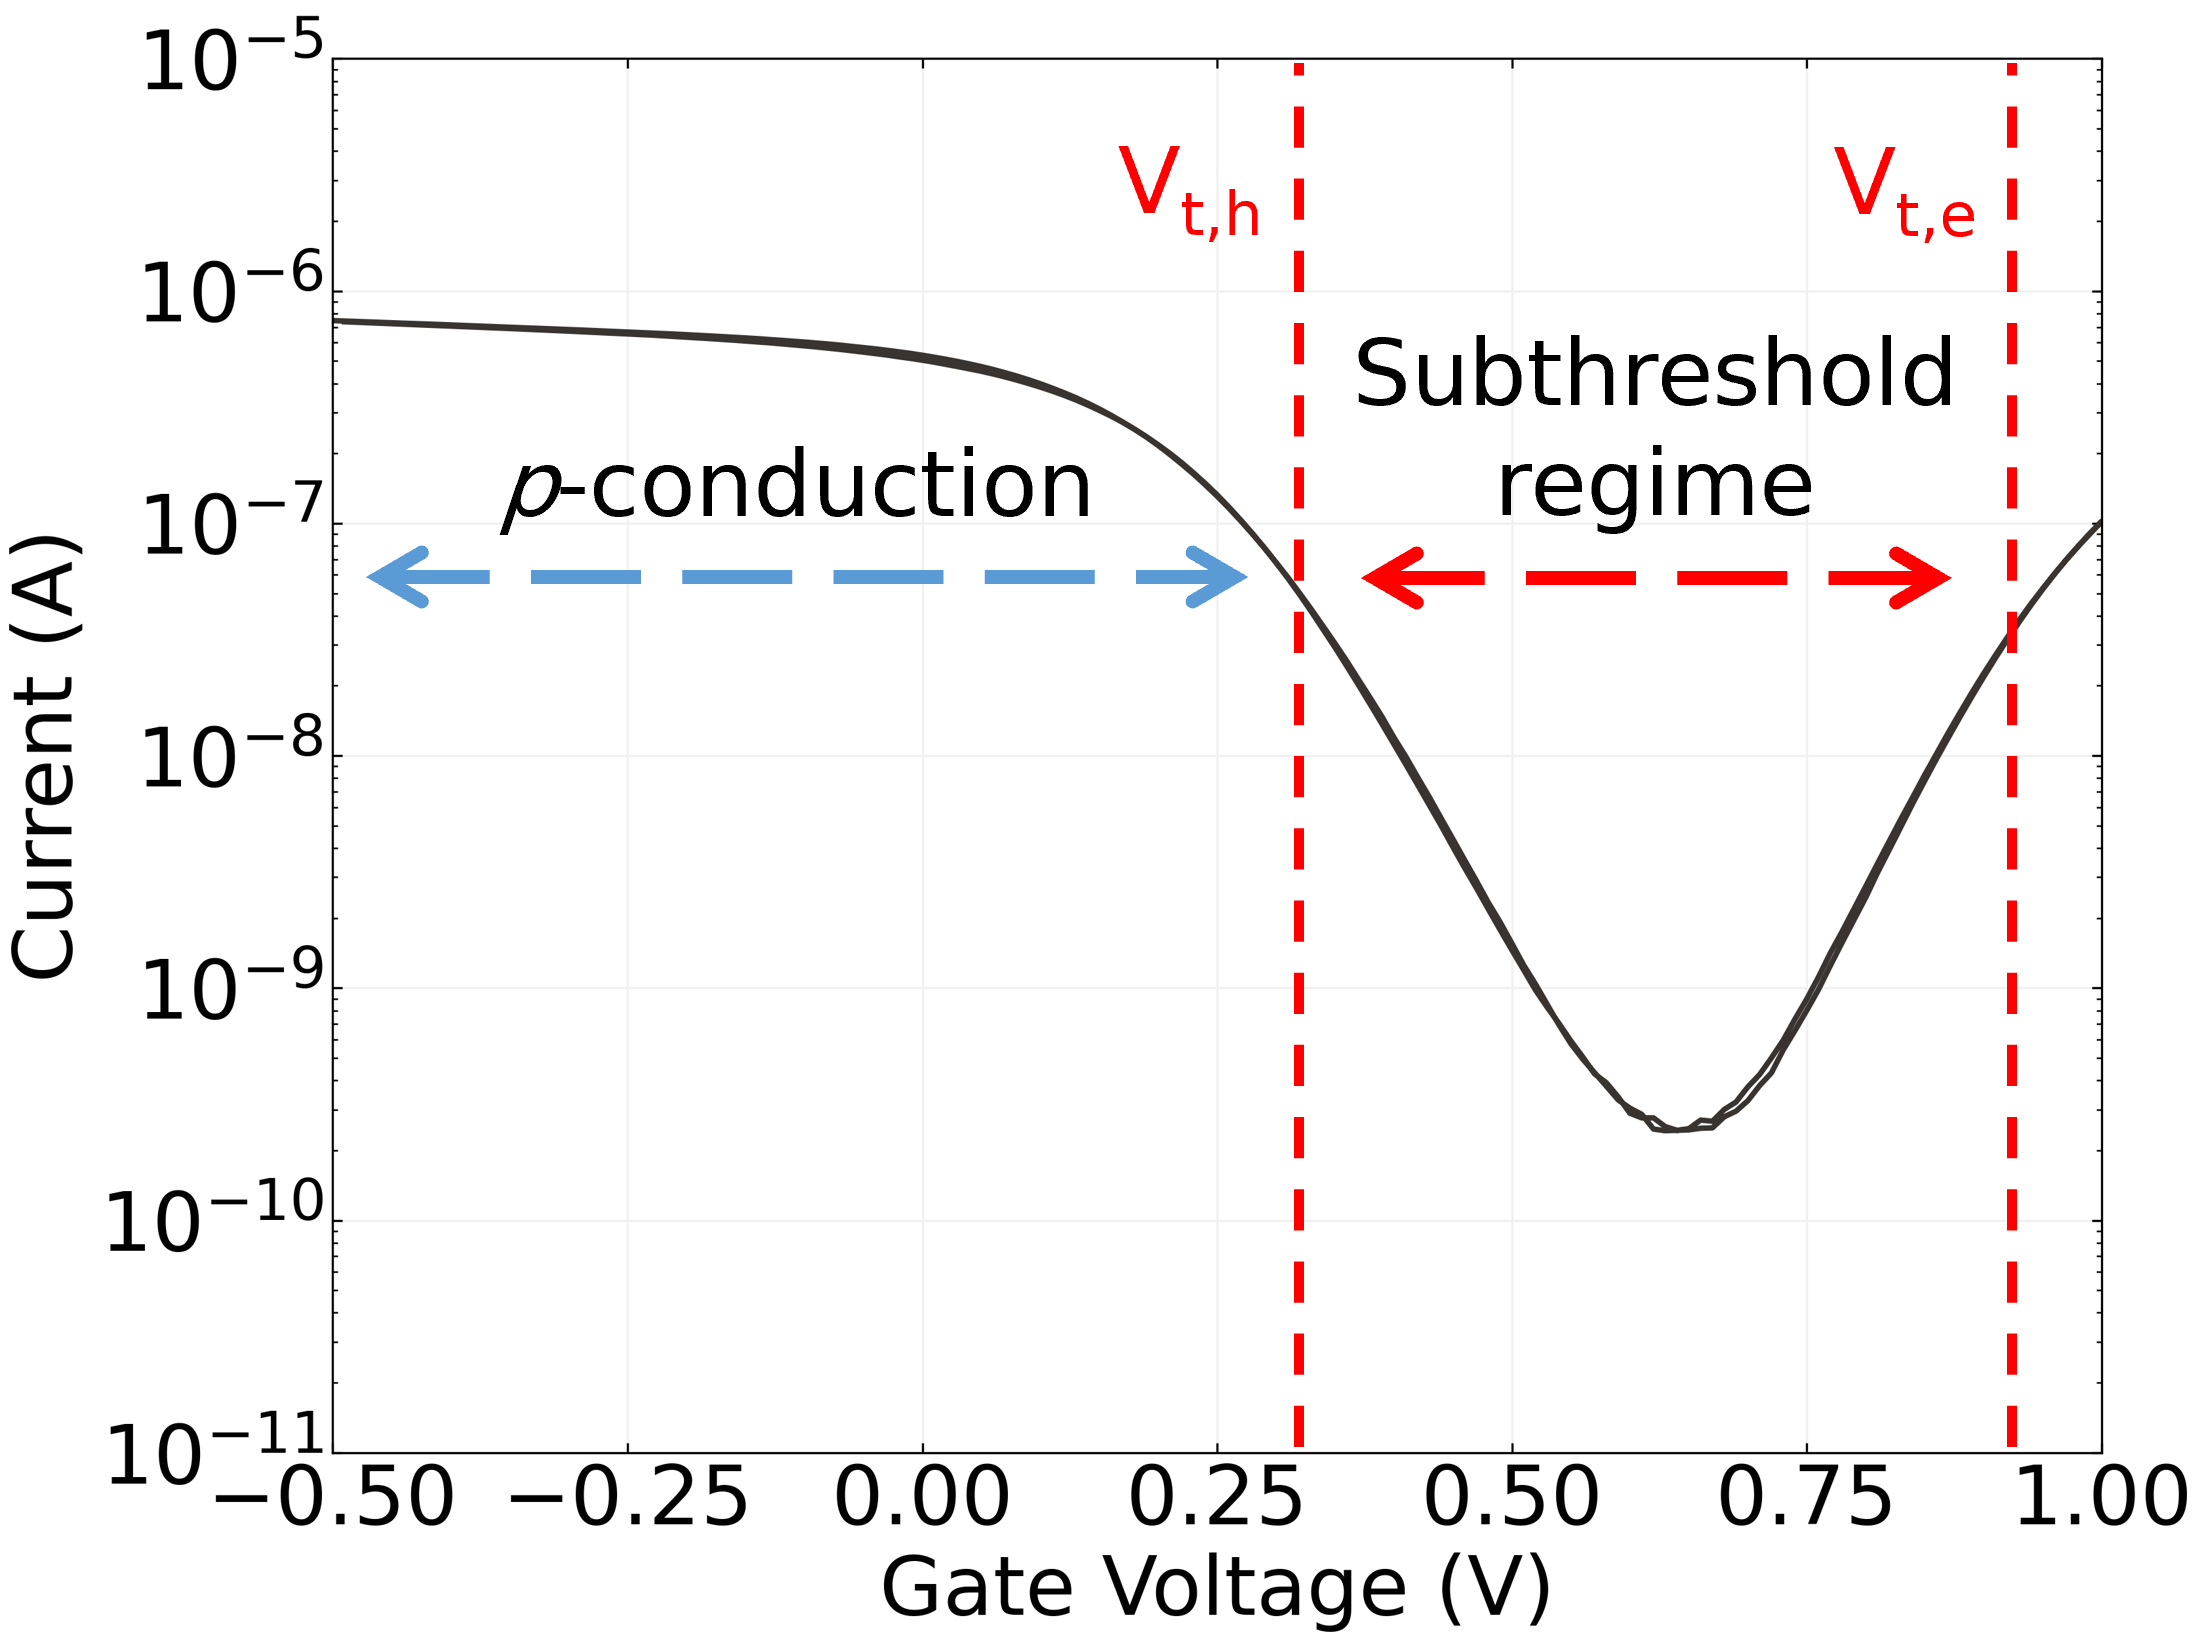
\includegraphics{figures/ch2/CNT_transfer_1.png}

}

}

\end{minipage}%
%
\begin{minipage}[t]{0.01\linewidth}

{\centering 

~

}

\end{minipage}%
%
\begin{minipage}[t]{0.03\linewidth}

{\centering 

\raisebox{-\height}{


\includegraphics{figures/(b).png}

}

}

\end{minipage}%
%
\begin{minipage}[t]{0.01\linewidth}

{\centering 

~

}

\end{minipage}%
%
\begin{minipage}[t]{0.45\linewidth}

{\centering 

\raisebox{-\height}{

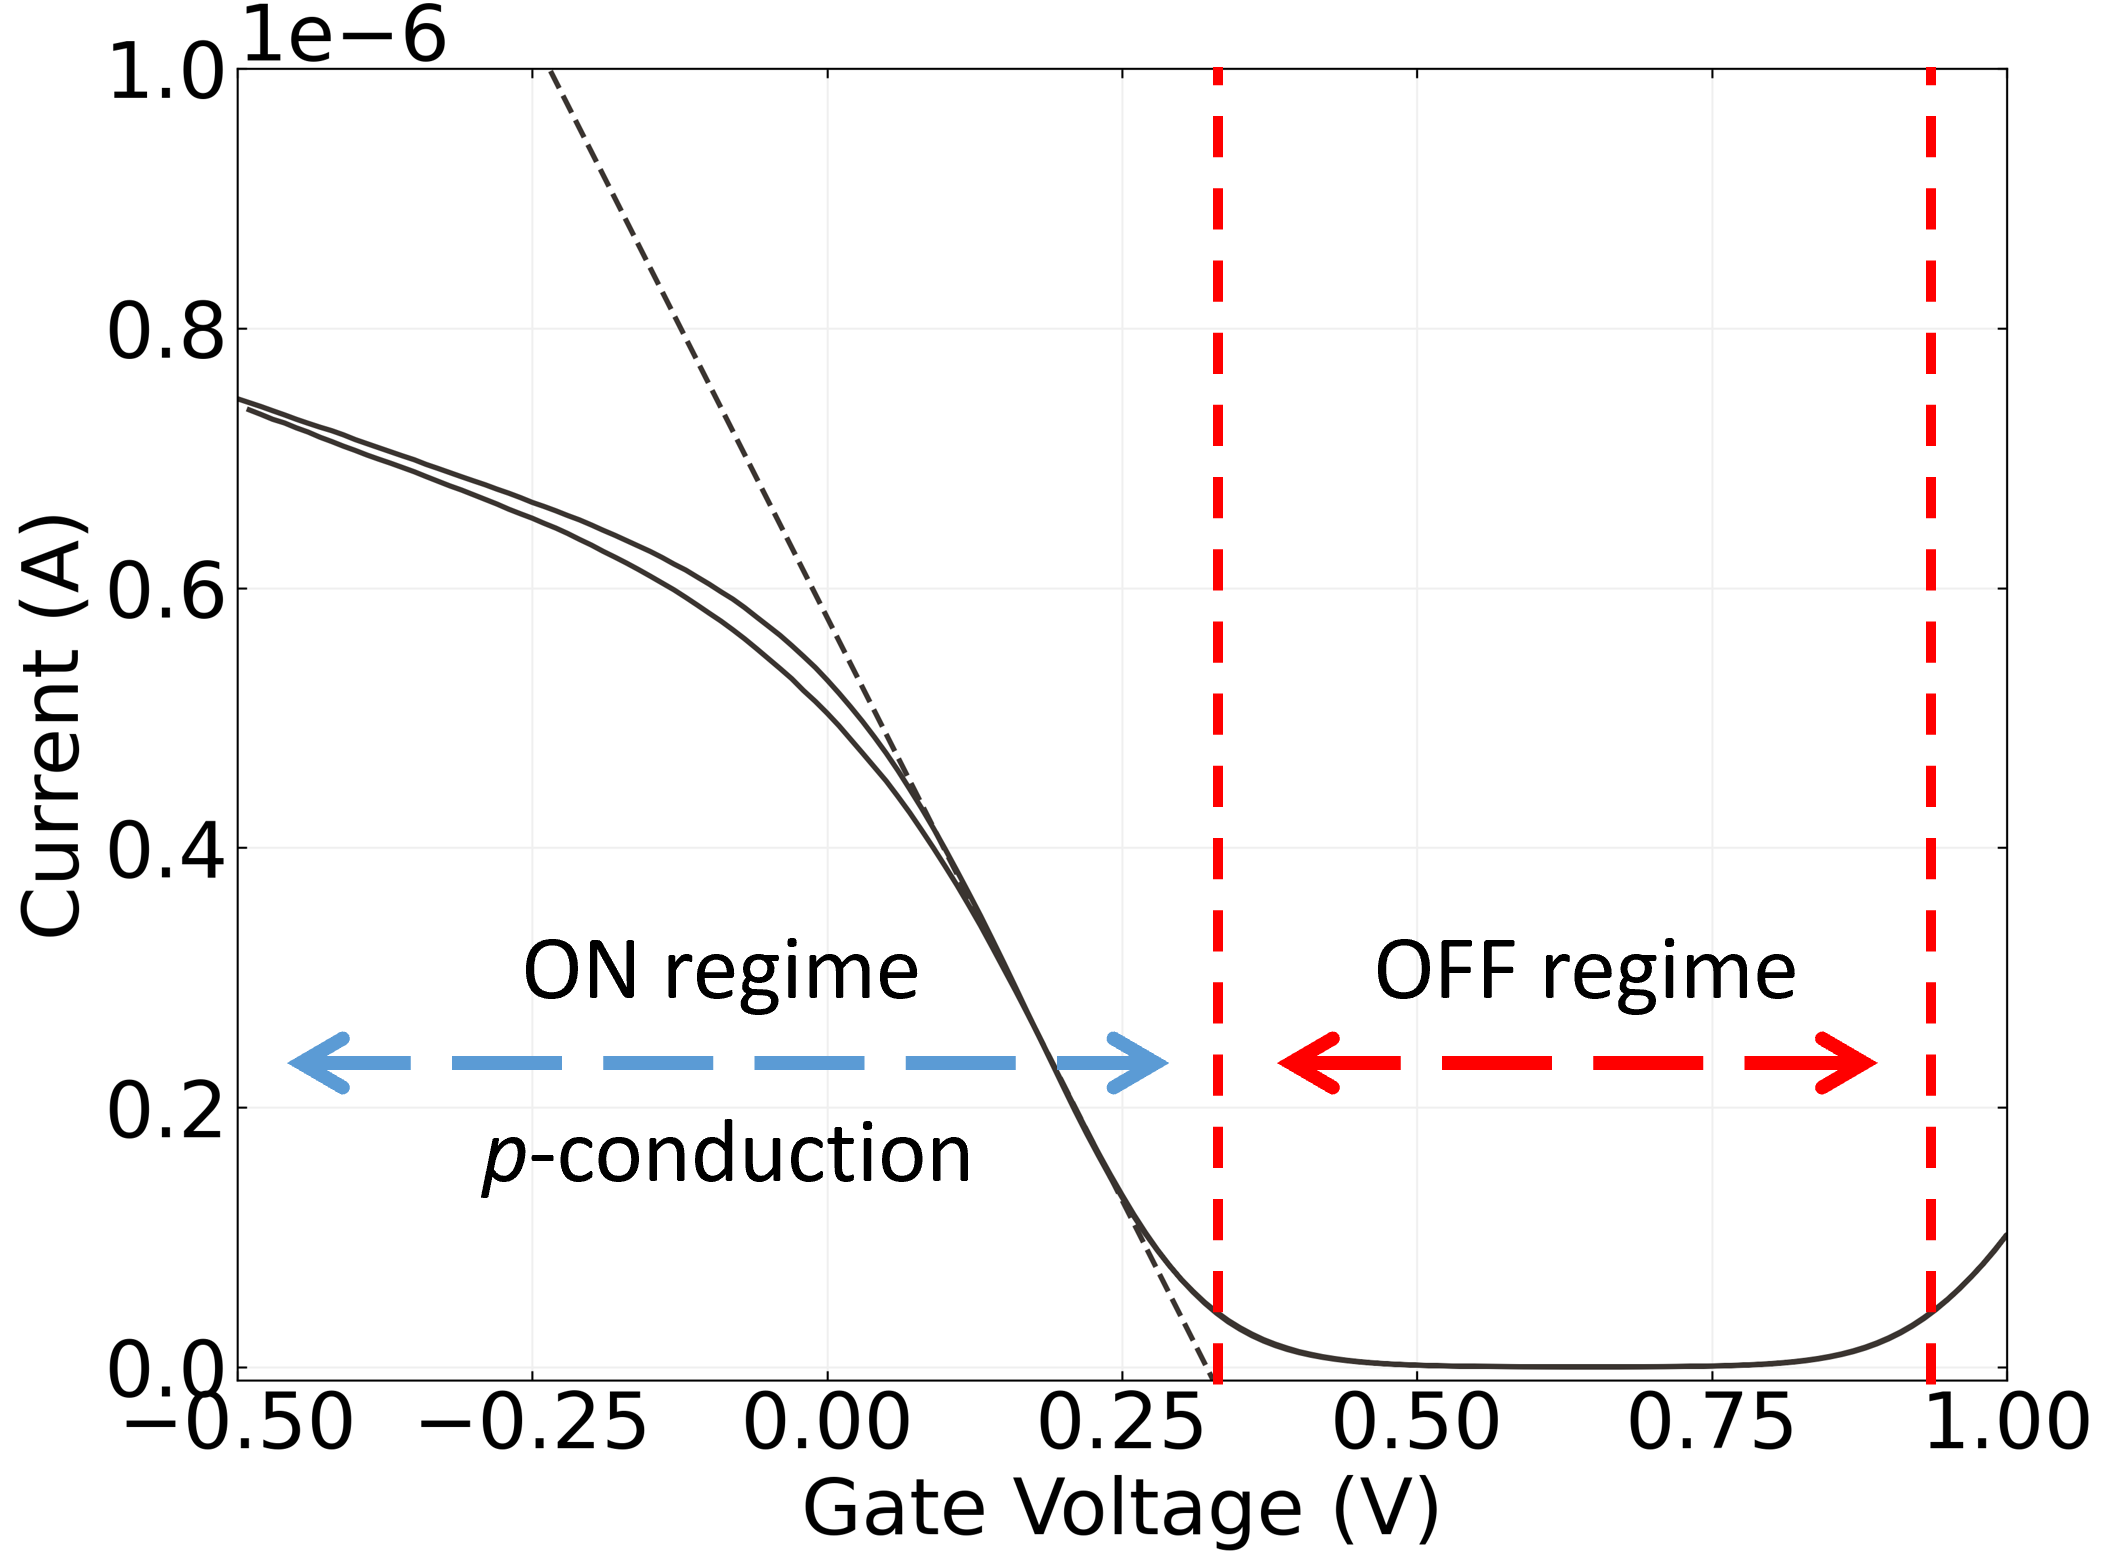
\includegraphics{figures/ch2/CNT_transfer_2.png}

}

}

\end{minipage}%
%
\begin{minipage}[t]{0.01\linewidth}

{\centering 

~

}

\end{minipage}%

\caption[Liquid-gated transfer characteristics of a CNT FET channel
showing the region of hole conduction and the subthreshold
regime.]{\label{fig-CNT-characteristics}Liquid-gated transfer
characteristics of a single carbon nanotube network field-effect
transistor channel, using a logarithmic scale in (a) and using a linear
scale in (b) to emphasise different features of the same dataset. The
subthreshold slope is shown with a black dotted line, while the
threshold voltages are shown with red dotted lines. The ON and OFF
regimes are also indicated on both figures. \(V_{ds}\) = 100 mV was
placed across the channel.}

\end{figure}

The threshold voltage \(V_t\) of a unipolar transistor is equal to the
gate voltage required to prevent the flow of charge carriers across the
channel, often referred to as turning the device off
\autocite{Petti2016,Shkodra2021}. In ambipolar devices, two separate
threshold voltages exist for each type of charge carrier, \(V_{t,h}\)
and \(V_{t,e}\), which are shown in Figure~\ref{fig-CNT-characteristics}
on both a linear (a) and logarithmic (b) scale. In the region between
these gate voltages, known as the subthreshold regime, both holes and
electrons flow through the channel
\autocite{Avouris2007,Reiner-Rozman2015}. If percolating pathways
consisting entirely of m-CNTs are present, \(I_{off}\) flows through
these pathways, as conduction through metallic nanotubes is largely
unaffected by changes in \(V_g\) \autocite{Fuhrer2000,Topinka2009}. If
there are no unblocked m-CNT pathways, \(I_{off}\) is entirely due to
Schottky barrier tunnelling \autocite{Avouris2007}. \(V_t\) can be
estimated by extrapolating the trendline of the linear region of the
transfer characteristics to the \(V_g\) axis. The intercept is
approximately equal to the threshold voltage when \(V_{ds}\) is close to
zero, as shown in Figure~\ref{fig-CNT-characteristics} (b)
\autocite{Sze2006,Petti2016,Li2023}. This is only a rough estimate of
the actual device \(V_t\), but is sufficient when comparing the gating
behaviour of different devices \autocite{Li2023}.

\begin{figure}

{\centering 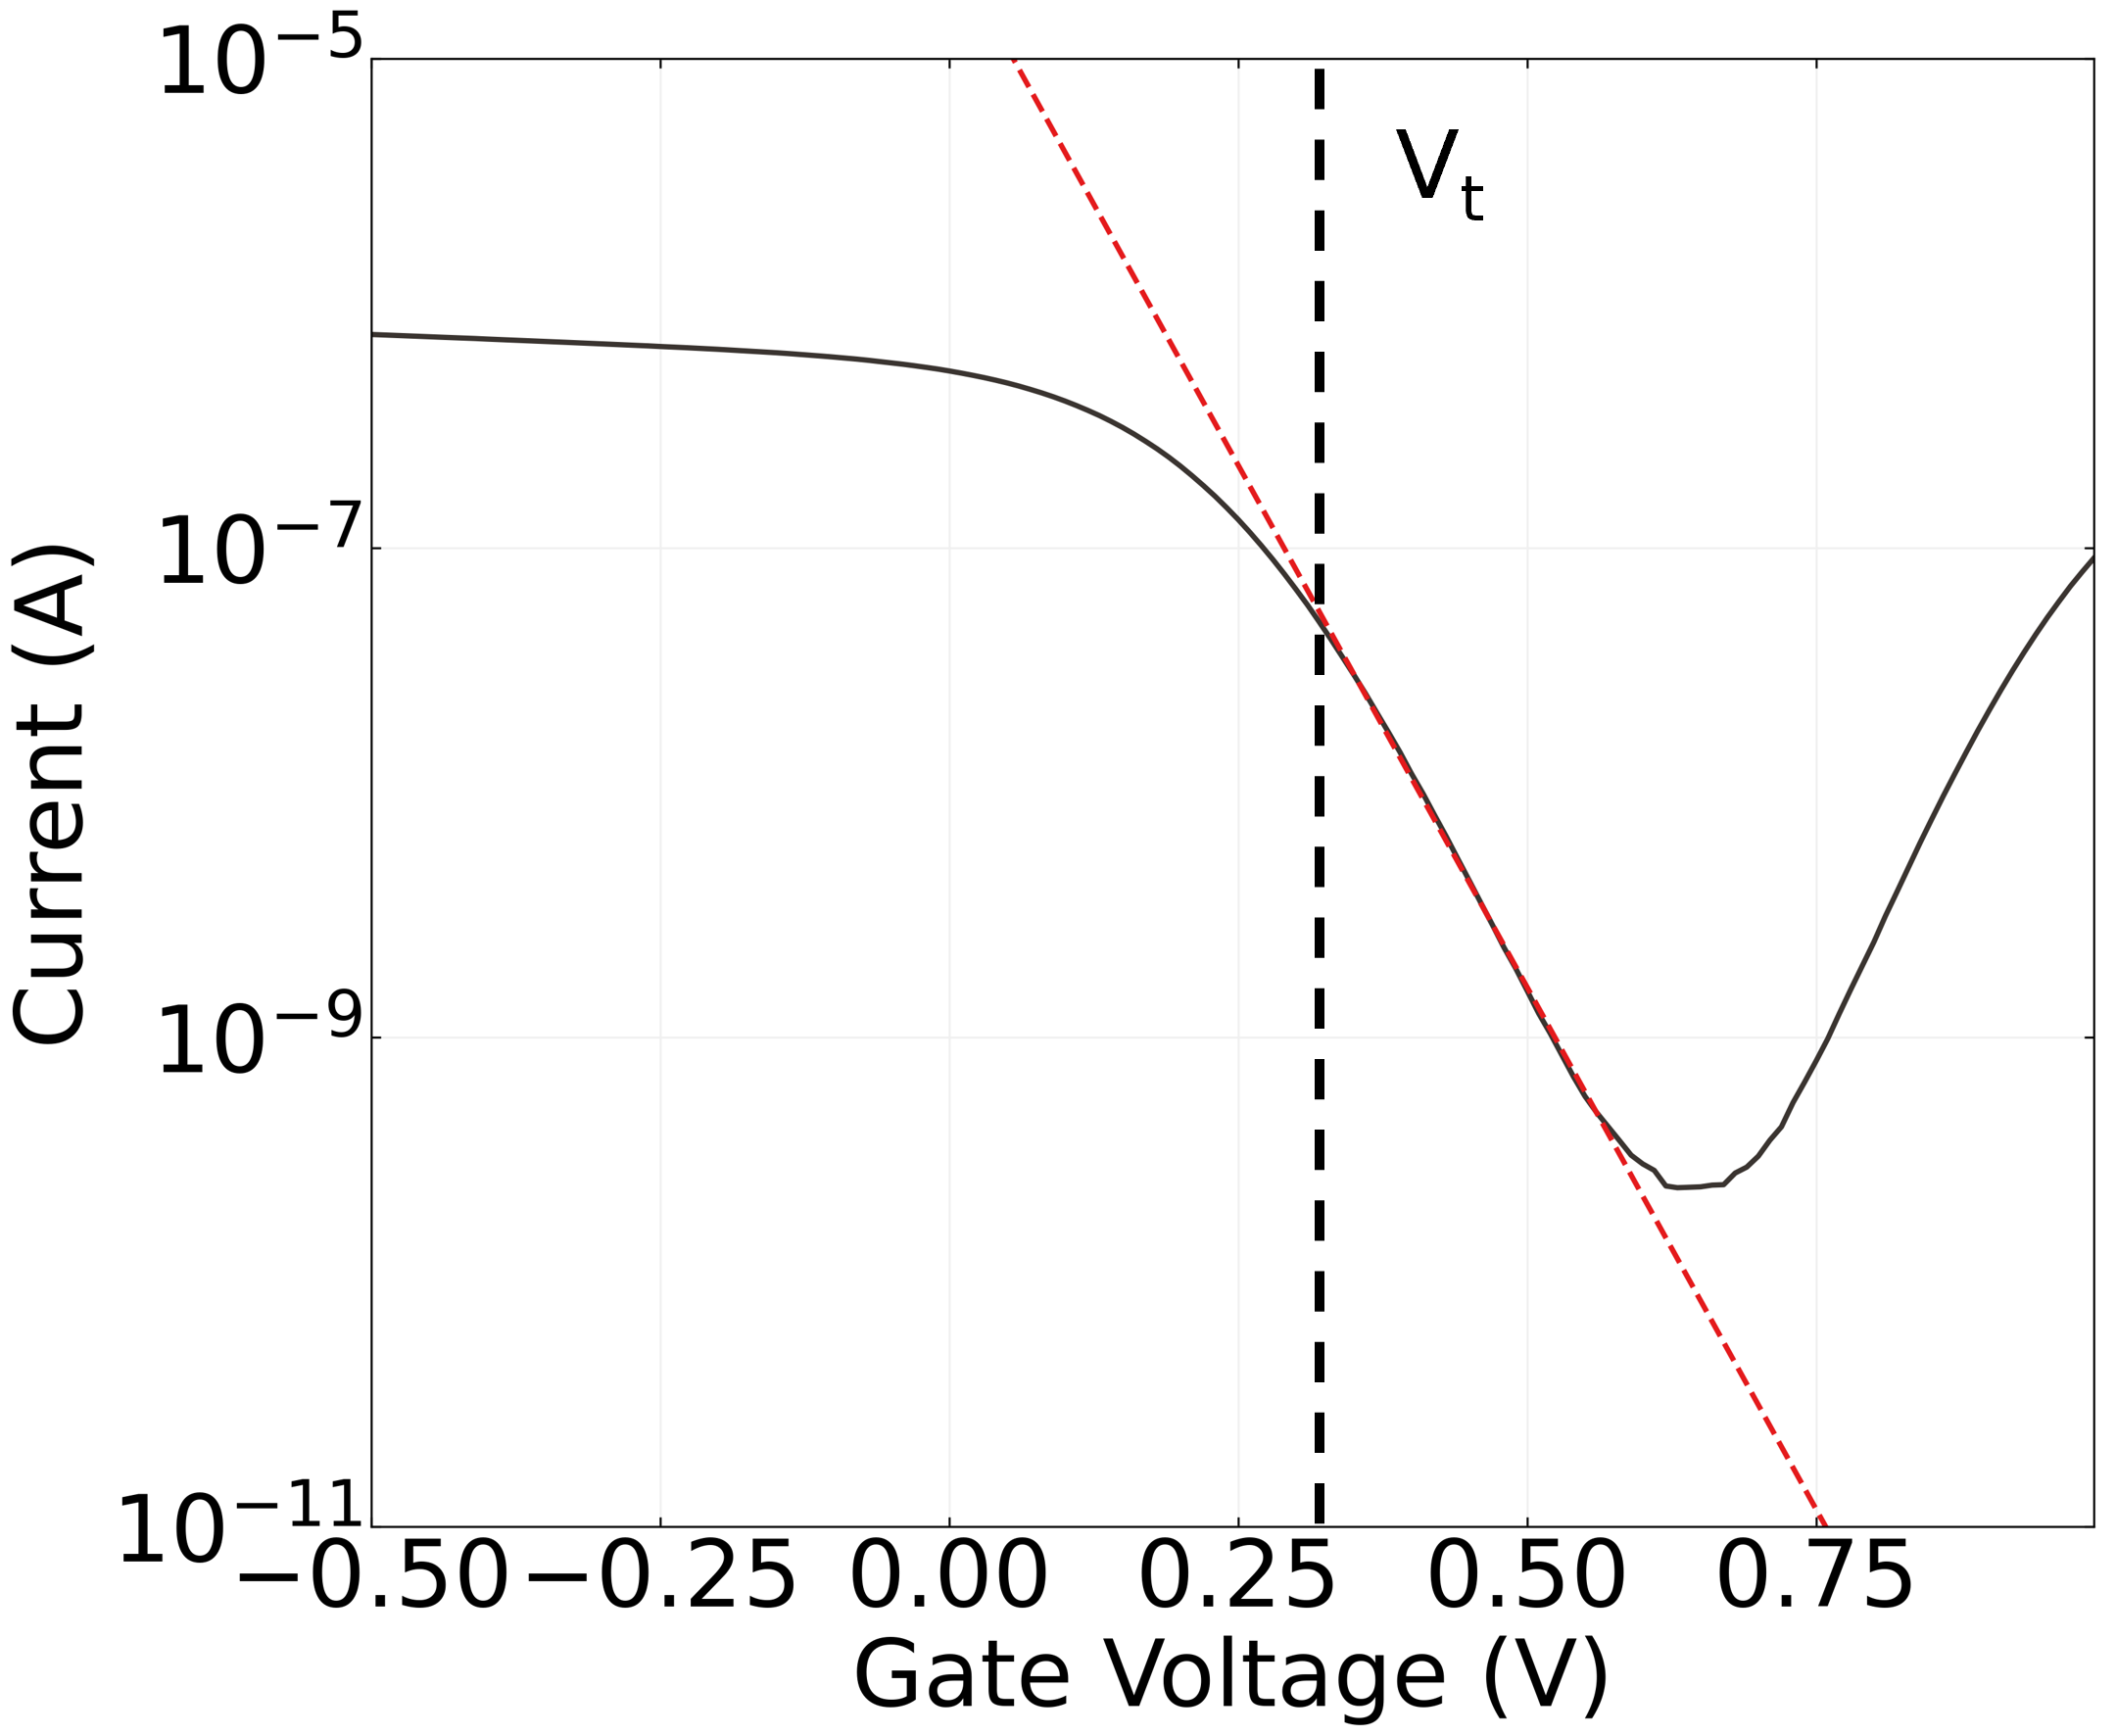
\includegraphics[width=0.45\textwidth,height=\textheight]{figures/ch2/NTQ31C5ch1subthreshold_slope_alt.png}

}

\caption[Liquid-gated transfer characteristics of a CNT FET channel on a
logarithmic scale, showing subthreshold slope and threshold
voltage.]{\label{fig-subthreshold-slope}A carbon nanotube network
transfer sweep with \(V_{ds}\) = 100 mV on a logarithmic scale.
Threshold voltage is shown with a black dotted line, while subthreshold
slope is shown with a red dotted line.}

\end{figure}

The subthreshold slope
\(S = d\textrm{log}_{10}(I_{d})/dV_g|_{\textrm{max}}\) is a measure of
how rapidly a transistor approaches the minimum current \(I_{off}\). The
subthreshold slope is often referred to using its reciprocal value, the
subthreshold swing, which is equivalent to the change in \(V_g\)
required to change \(I_d\) by one order of magnitude. This figure of
merit is strongly related to the gate capacitance of the device. As the
slope exponentially approaches the off current in the subthreshold
regime, it can be fitted with a linear trendline on a logarithmic scale.
\autocite{Sze2006,Petti2016}. A linear trendline fitted to the logarithm
of the subthreshold regime is shown in
Figure~\ref{fig-subthreshold-slope}, where the gradient corresponds to
subthreshold slope. A high subthreshold slope exceeding than 10
decades/V is preferred for reduced power consumption of the working
sensor device \autocite{Petti2016}. The subthreshold slope of the
transfer sweep in Figure~\ref{fig-subthreshold-slope} is 8 decades/V.
Heller \emph{et al.} and Gao \emph{et al.} found that sensor devices
showed better signal-to-noise ratio when gated in the subthreshold
regime, as small voltage changes in response to analyte led to
exponential current changes along the subthreshold slope
\autocite{Heller2009,Gao2010}.

\hypertarget{sec-CNT-sensing-mechanisms}{%
\subsection{Sensing}\label{sec-CNT-sensing-mechanisms}}

As all atoms are at the surface of the carbon nanotube structure,
nanotubes are very sensitive to their surroundings and easily modified,
making them useful in biosensor applications
\autocite{Cao2009,Yao2021,Shkodra2021}. The chirality and diameter of a
carbon nanotube affects both its coupling with the gate and its surface
chemistry, which determines the sensing mechanisms available to a single
CNT. Only s-CNTs can be electrostatically gated; m-CNTs, bent nanotubes
and larger diameter nanotubes are typically more reactive
\autocite{Cao2009,Zhao2012,Chhikara2013,Li2023}; and the nanotube
chirality (\(n, m\)) can determine the strength of binding to DNA in a
base sequence-dependent manner \autocite{Rouhi2011a}. Carbon nanotubes
have been used for vapour-phase sensing since 2000, when Kong \emph{et
al.} found that the resistance over a single CNT channel was modified
when exposed to gas molecules like NO\(_2\) and NH\(_3\)
\autocite{Kong2000}. Carbon nanotubes have been used to detect the
presence of analyte down to the parts per billion level in a variety of
gas sensor applications \autocite{Chen2019,Yao2021}. However, in
general, the specificity of such a sensor is low, as nanotubes respond
to many different analytes in a similar manner. To enhance specificity,
surface functionalisation is often performed using either inorganic or
biological materials, such as enzymes, antibodies, aptamers and proteins
\autocite{Cao2009,Shkodra2021,Yao2021}.

For carbon nanotube network transistors, sensing mechanisms include
electrostatic gating, charge transfer, Schottky barrier modulation,
modulation of channel capacitance relative to the electrolyte and charge
scattering. Response mechanisms may take place at the gate, the
junctions between channel and contact, or at the semiconductor channel
\autocite{Heller2008,Battie2011,Boyd2014,Tran2016,Li2023}. Modification
of the channel-metal Schottky barrier can dominate sensing activity, and
this can complicate the identification of mechanisms underlying the
sensing behaviour \autocite{Cao2009,Boyd2014,Schroeder2019}. The
encapsulation layer shown in Figure~\ref{fig-gating-schematics} is added
to separate the electrodes from the channel-metal junction and prevent
these responses \autocite{Heller2008,Shkodra2021}. In an encapsulated
device, the predominant sensing mechanism is either charge transfer from
the analyte to channel \autocite{Allen2007,Battie2011} or electrostatic
gating \autocite{Heller2008}. The charge transfer mechanism involves
direct addition of charge carriers to the channel, while the gating
mechanism results from a nearby charge inducing an opposite polarity
charge in the channel. Both changes alter the relationship between
\(V_g\) and \(I_d\) and shift the carrier threshold voltage(s)
\autocite{Tran2016,Shkodra2021,Li2023}. Modulation of Schottky and other
potential barriers present in the network may also make a significant
contribution to sensing responses, especially when a network is close to
its percolation threshold \autocite{Boyd2014,Murugathas2019}.

\hypertarget{summary}{%
\section{Summary}\label{summary}}

Graphene and carbon nanotube network field-effect transistors were
explored as the transducer element for vapour-phase biosensors due to
their low cost, small size and high sensitivity. Important device
parameters of the graphene and carbon nanotube network FETs include
transconductance, on-off ratio, gate leakage currents, current
hysteresis, threshold voltage and sub-threshold slope. The voltage
corresponding to the Dirac point (or points) of graphene is another
important figure of merit for graphene field-effect transistors. Various
attributes of the morphology of graphene and carbon nanotube networks
contribute to the unique electrical and sensing properties exhibited by
these transistors, including graphene folds and junctions between
nanotubes of different chirality. Research continues into optimising the
device morphology of thin-film FETs for maximum sensitivity, where the
the use of monolayer graphene and highly-purified s-CNT networks for the
thin-film are more recent developments in the field. Further exploration
of the relationship between thin-film morphology and transistor
characteristics can be found in
Chapter~\ref{sec-pristine-characteristics}.

Although the extreme sensitivity of these thin-film transistors is well
known, the use of these sensors for detection of specific compounds is
an area of ongoing research. In the past few decades, a focus of
investigation has been chemical and biological decoration of these
transistors to produce selective responses to compounds of interest.
Though there are a broad range of chemical and biological modifications
available for this purpose, this work focuses on the nature-inspired use
of insect odorant receptors for selective detection. The previous use of
thin-film transistors functionalised in this manner to produce a
specific sensing response to volatile compounds is described in detail
in Chapter~\ref{sec-iOR-sensors}. There is also ongoing debate regarding
the precise mechanisms underlying sensing responses from these
transducers, particularly with respect to detection of vapour-phase or
gaseous compounds. A discussion of vapour-phase sensing with pristine
carbon nanotube thin-film transistors can be found in
Chapter~\ref{sec-pristine-characteristics}.

\bookmarksetup{startatroot}

\hypertarget{sec-iOR-sensors}{%
\chapter{Biosensing with Insect Odorant
Receptors}\label{sec-iOR-sensors}}

\hypertarget{sec-biosensing-transducers}{%
\section{Introduction}\label{sec-biosensing-transducers}}

In Chapter~\ref{sec-thin-film-transistors}, it was established that as
carbon nanotubes and graphene are extremely sensitive and are easily
modified with biomaterials, they are a highly suitable platform for
biosensing \autocite{Kauffman2008,Ohno2010}. In the early 2000s, it was
established that sensitive and selective biosensors could be created by
modifying a carbon nanotube field-effect transistor channel with protein
receptors \autocite{Chen2003,Kauffman2008}. In the following two
decades, a wide range of other biological receptors have been attached
to carbon nanotube FETs and graphene FETs for the creation of
biosensors, including enzymes \autocite{Lee2009,Zhang2015a,Dudina2019},
antibodies \autocite{Kim2008,Jin2015,Tsang2019} and aptameric DNA
\autocite{Maehashi2007,Gao2016,Nguyen2021}. These miniaturised ``lab on
a chip'' devices are of particular interest due to their reliability,
low cost, rapid use time, simple operation and small size compared with
alternative spectroscopic or fluorescence-based sensing methods
\autocite{Khan2020}. It is hoped that such sensors could be deployed
outside the laboratory in a range of front-line settings which require
rapid and reliable detection \autocite{Dung2018,Yang2018,Kim2022a}.

Rapid developments in this biosensor technology and parallel
developments in the understanding of animal olfaction led to these
transistors being used in bioelectronic nose applications from the late
2000s onwards \autocite{Yoon2009,Jin2012,Lee2012b,Park2012}.
``Bioelectronic nose'' is a general term dating back to 1961, which
refers to the use of an biologically-modified electronic array to detect
specific odor traces in a highly selective and sensitive manner. As the
name suggests, the signals from this system mimic the electrochemical
signals received by olfactory neurons in an animal nose
\autocite{Glatz2011,Dung2018}. A biomimetic approach to bioelectronic
nose development couples the CNT FET or GFET signal-amplifying
transducer element with sensitive components of the animal olfactory
system. These components include olfactory cells \autocite{Wang2007},
odorant binding proteins (OBPs) \autocite{Larisika2015,Kotlowski2018}
and odorant receptor proteins (olfactory receptors, ORs)
\autocite{Yang2018,Murugathas2020}. An bioelectronic nose can discern
specific volatile odors in the air at low parts-per-trillion
concentrations \autocite{Lee2010,Moon2020}. This performance is far
superior to commercially-available vapour-phase sensors, which are at
best only responsive down to parts-per-billion concentrations
\autocite{GasDetector1,GasDetector2}. The aim for novel olfactory-based
electronic biosensors is to match or surpass this level of selective
accuracy to volatile organic vapours
\autocite{Glatz2011,Kwon2015,Dung2018,Bohbot2020,Kim2022a}.

\hypertarget{sec-odorant-receptors-biosensors}{%
\section{Odorant Receptors in Field-Effect Transistor
Biosensors}\label{sec-odorant-receptors-biosensors}}

\hypertarget{sec-odorant-receptors}{%
\subsection{Odorant Receptors}\label{sec-odorant-receptors}}

Odorant receptors (ORs) are an essential part of the olfactory systems
of most animals, including humans. ORs let us distinguish between
thousands of odors \autocite{Buck1991,Dung2018,Yang2018,Kim2022a}.
Vertebrate odorant receptors are part of a group of seven-transmembrane
proteins known as G-protein coupled receptors (GPCRs)
\autocite{Buck1991,Glatz2011,Dung2018,Wicher2021}. Compounds entering a
vertebrate nose selectively bind to specific odorant receptors, which
undergo a change in conformation \autocite{Dung2018,Kim2022a}. The
binding process leads to activation and dissociation of the G-protein
within the neuronal cell. Intracellular signalling events triggered by
G-protein dissociation are converted to an action potential which is
then transmitted to the brain \autocite{Buck1991,Glatz2011,Zhang2021}.
The combination of activated receptors is then interpreted as a specific
odor \autocite{Sato2014,Kwon2015,Hurot2020,Kim2022a}. Odorant receptors
may be activated by a few or many target (or ``agonist'') compounds. The
target compounds are determined by subtle differences in OR amino acid
composition \autocite{Carraher2015,Yang2018,Goodwin2021}. An
``antagonist'' compound may inhibit the response of a receptor to other
compounds \autocite{Lee2012,Carraher2015}. Compounds which trigger a
strong signal from a specific odorant receptor are often referred to as
``positive ligands'' for that receptor, while those that cause no
response are ``negative ligands''
\autocite{Murugathas2019a,Murugathas2020,Yoo2022}.

\hypertarget{sec-artificial-membranes}{%
\subsection{Artificial Membranes}\label{sec-artificial-membranes}}

Odorant receptors are transmembrane proteins, which are insoluble and
tend to aggregate and oligomerise in solution \autocite{Nath2007}. They
therefore require stabilisation from either a specific detergent
environment or a membrane layer to preserve their structure and function
when solubilised \autocite{Fruh2011,Dung2018}. Odorant receptors can be
expressed and isolated using heterologous cell systems, where a host
cell replicates a protein from transfected RNA or DNA material
\autocite{Glatz2011,Dung2018}. The most commonly used expression cells
are human embryonic kidney (HEK) cells \autocite{Lim2014,Ahn2020},
\emph{E. Coli} bacteria \autocite{Yang2017,Yang2018} and \emph{S.
cerevisiae} (baker's yeast) \autocite{Bohbot2020}. The cell membrane can
then be used directly in a sensor \autocite{Dung2018}. Alternatively,
odorant receptors can be embedded in an artificial lipid membrane format
that mimics the native cell membrane \autocite{Nath2007}. These
membranes can be produced in large numbers and remain in storage for
much longer than live cells \autocite{Goldsmith2011,Lim2015}. Lipid
membranes are constructed from phospholipid molecules, which comprise of
a small, hydrophilic, polar ``head'' and long, hydrophobic, non-polar
``tail'' \autocite{Bose2021,Ramadon2022}. These artificial membranes
include detergent micelles, nanovesicles (including liposomes), and
nanodiscs \autocite{Yang2018,Moon2020}. The small size of these
artificial membranes makes them appropriate for use with
nanomaterial-based transducers \autocite{Lim2015,Dung2018}.

\begin{figure}

\begin{minipage}[t]{0.03\linewidth}

{\centering 

\raisebox{-\height}{


\includegraphics{figures/(a).png}

}

}

\end{minipage}%
%
\begin{minipage}[t]{0.01\linewidth}

{\centering 

~

}

\end{minipage}%
%
\begin{minipage}[t]{0.55\linewidth}

{\centering 

\raisebox{-\height}{

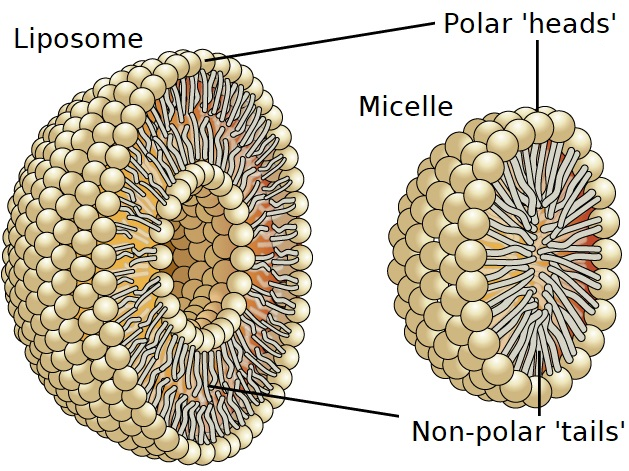
\includegraphics{figures/ch3/OSC_Microbio_07_03_micelle_edit.png}

}

}

\end{minipage}%
%
\begin{minipage}[t]{0.01\linewidth}

{\centering 

~

}

\end{minipage}%
%
\begin{minipage}[t]{0.03\linewidth}

{\centering 

\raisebox{-\height}{


\includegraphics{figures/(b).png}

}

}

\end{minipage}%
%
\begin{minipage}[t]{0.01\linewidth}

{\centering 

~

}

\end{minipage}%
%
\begin{minipage}[t]{0.36\linewidth}

{\centering 

\raisebox{-\height}{

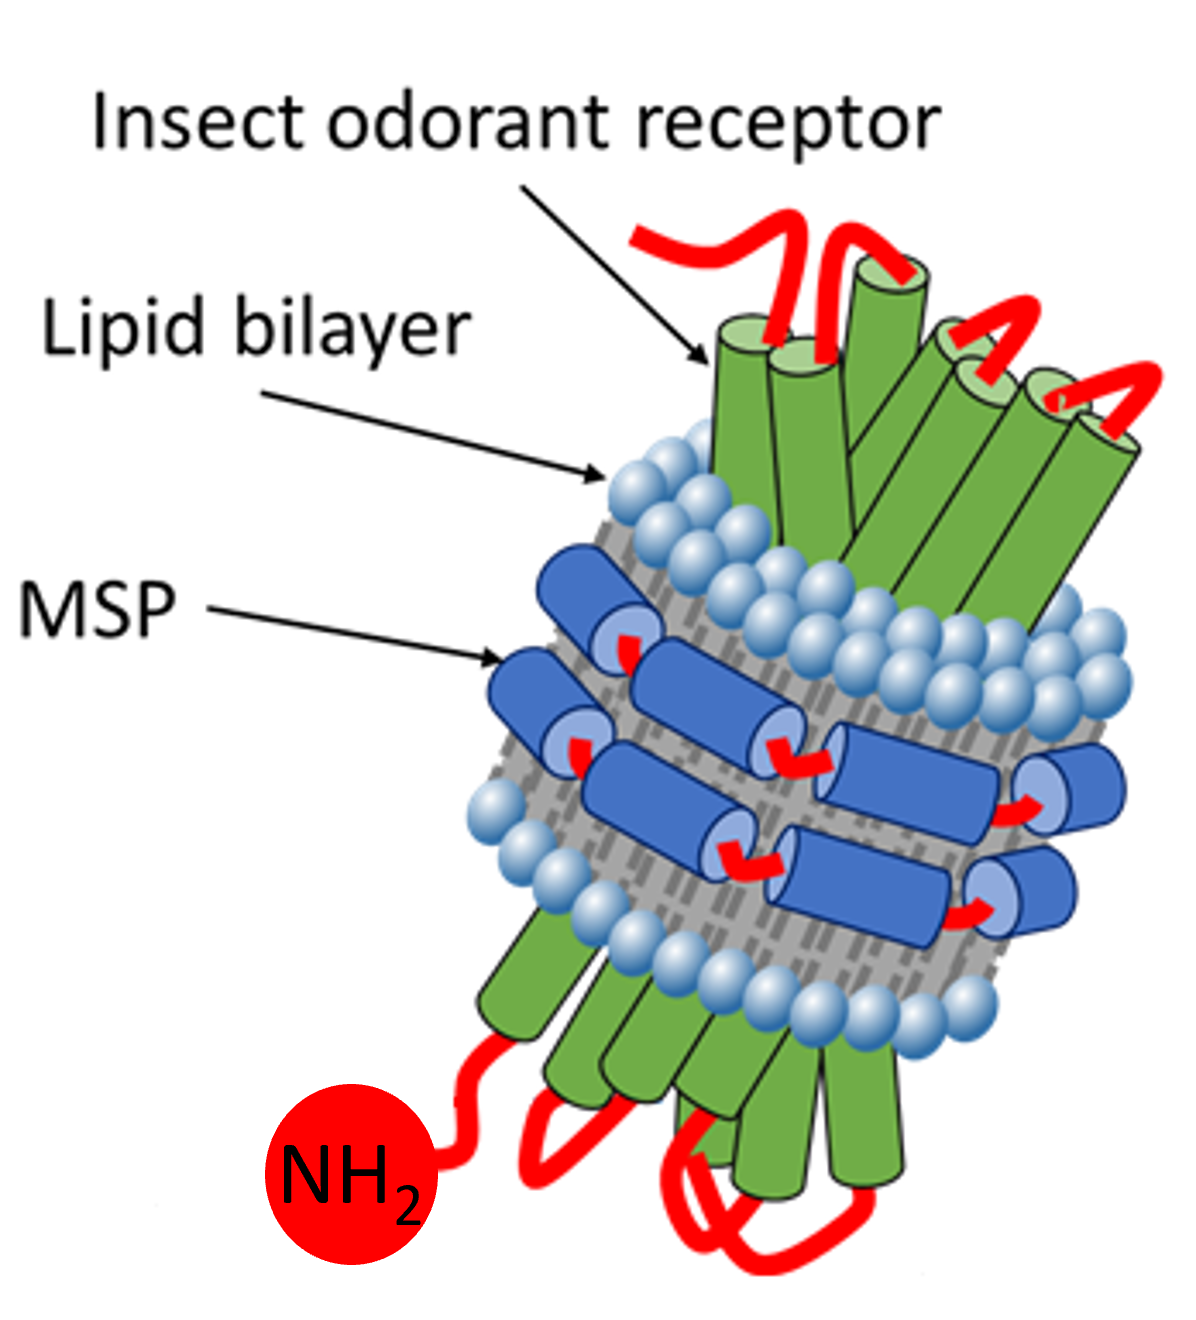
\includegraphics{figures/ch3/iOR_nanodisc.png}

}

}

\end{minipage}%
%
\begin{minipage}[t]{0.01\linewidth}

{\centering 

~

}

\end{minipage}%

\caption[Diagrams showing the structure of various artificial
membranes.]{\label{fig-membranes}Liposomes and micelles are shown in (a)
with the hydrophilic heads and hydrophobic tails indicated. A lipid
nanodisc wrapped around an insect odorant receptor transmembrane protein
is shown in (b), where the amine group shown is the odorant receptor
N-terminus. The nanodisc consists of a lipid bilayer encircled by a
membrane scaffold protein (MSP). Images are not to scale. The schematic
in (a) is adapted from \autocite{Micelle}, and used under the CC BY-4.0
license. The schematic in (b) is reprinted with permission from
\autocite{Murugathas2019a}. Copyright \(\copyright\) 2019 American
Chemical Society.}

\end{figure}

A nanovesicle is a nanoscopic spherical bilayer fluid sac. There are
various types of artificial nanovesicles, including liposomes,
ethosomes, transfersomes, niosomes and phytosomes. The type of
nanovesicle depends on its chemical makeup \autocite{Ramadon2022}. For
example, a liposome is made up of phospholipid and cholesterol, and can
consist of one or more concentric amphiphilic bilayers. The liposome can
contain hydrophobic compounds within the bilayer due to hydrophobic
interactions, while hydrophilic compounds are held within the vesicle
core or interior \autocite{Nath2007,Ramadon2022}. A nanovesicle can be
used solely as a format to protect membrane proteins
\autocite{Murugathas2020}, or with the addition of integrated ion
channels, can mimic the operation of a cell \emph{in vivo}, with
intracellular signalling pathways triggered by the membrane proteins
\autocite{Lim2015}. Nanomicelles (or simply micelles) are also
nanoscopic and spherical, but unlike nanovesicles have no inner fluid
sac \autocite{Nath2007,Bose2021}. Micelles self-assemble when
phospholipid is mixed with detergent. The surface of the micelle is made
up of the hydrophilic detergent and phospholipid heads, while the
internal core is made up of the hydrophobic phospholipid tail
\autocite{Nath2007}. Hydrophobic compounds can be contained within the
core of the micelle \autocite{Bose2021}. Figure~\ref{fig-membranes} (a)
illustrates the difference between the liposome and micelle structures.

Nanodiscs have emerged as a model membrane candidate which has many
advantages over the more traditional nanovesicle and micelle formats.
The nanodisc is a disc-shaped lipid bilayer encompassed by an membrane
scaffold protein (MSP), with structure pictured in
Figure~\ref{fig-membranes} (b) \autocite{Nath2007,Bayburt2010,Yang2018}.
The amphiphilic membrane scaffold protein protects the exposed, strongly
hydrophobic side chains of the nanodisc in an aqueous environment
\autocite{Fruh2011,Yang2018}. Unlike liposomes and micelles, there is
little variation between the size of individual nanodiscs due to
constraints placed on the bilayer by the encompassing scaffold protein
used, meaning greater consistency within and between membrane batches
\autocite{Nath2007,Fruh2011}. Nanodiscs have also been found to be
significantly less prone to non-specific binding (see
Section~\ref{sec-non-specific-binding}) than micelles
\autocite{Fruh2011}. Another advantage of nanodiscs is that the membrane
scaffold protein can be attached to biosensor surfaces at specific
affinity tags, for example, the scaffold protein hexahistidine tag
(his-tag) \autocite{Bayburt2010,Fruh2011}. Depending on the type of MSP
used, a nanodisc measures between 10-20 nm across and can hold either a
single or several odorant receptors \autocite{Nath2007,Bayburt2010}. The
protein coating of the nanodisc makes it particularly stable. The
stability of nanodiscs means they can be used to produce particularly
reliable and long-lived biosensor devices
\autocite{Goldsmith2011,Yang2018,Moon2020,Cheema2021}.

\hypertarget{sec-sensor-types}{%
\subsection{Sensor Functionalisation}\label{sec-sensor-types}}

For a bioelectronic nose to operate, sufficient coupling must exist
between the bioreceptor element and the graphene or carbon nanotube
channel of the field-effect transistor. Odorant receptors can be
directly attached by physical adsorption; however, this approach is
difficult to control, and can lead to weak coupling between the odorant
receptors and the transducer \autocite{Kwon2015,Dung2018,Bohbot2020}.
Alternatively, a bifunctional linker element may mediate the attachment
between functional groups of the bioreceptor and the transducer in a
biochemical process referred to as ``functionalisation''
\autocite{Star2003a}. Functionalisation may involve covalent or
non-covalent bonding to the carbon-ring transducer surface. Covalent
bonding is stronger than non-covalent bonding, and therefore gives a
more permanent attachment between linker molecules and the transducer.
Unlike covalent attachment, non-covalent attachment preserves the
polycyclic \(sp^2\) bonding of carbon atoms in graphene and carbon
nanotubes and therefore the electrical properties of the channel
\autocite{DiCrescenzo2014,Yao2021,Shkodra2021,Li2023}. For example, one
group found covalent bonding of diazonium linker caused a \(\sim 50\) \%
drop in graphene channel mobility \autocite{Lerner2014}. In comparison,
only a \(\sim 5\) \% drop in mobility was seen for attachment of a
mixture of linkers containing pyrene to a graphene channel via
non-covalent pi-stacking \autocite{Thodkar2021}. The relative advantages
and disadvantages of each type of receptor immobilisation can be found
in Table~\ref{tbl-functionalisation-types}.

Table~\ref{tbl-or-biosensors} summarises all published odorant receptor
functionalised carbon nanotube and graphene field-effect
transistor-based sensors to date. The majority of published works on
this topic come from the Tai Hyun Park group at Seoul National
University.

\hypertarget{tbl-functionalisation-types}{}
\begin{longtable}[t]{>{\raggedright\arraybackslash}p{5.4cm}>{\raggedright\arraybackslash}p{1.45cm}>{\raggedright\arraybackslash}p{1.3cm}>{\raggedright\arraybackslash}p{1.45cm}>{\raggedright\arraybackslash}p{1.3cm}>{\raggedright\arraybackslash}p{1.3cm}}
\caption{\label{tbl-functionalisation-types}A comparison of the advantages and disadvantages of different approaches
for immobilising odorant receptors onto thin-film transducers. }\tabularnewline

\toprule
Attachment Type & Simplicity & Synergy & Specificity & Stability & Strength\\
\midrule
Direct Adsorption & High & Medium & Low & Low & Low\\
Linker, covalently tethered & Medium & Low & High & High & High\\
Linker, non-covalently tethered & Medium & High & Medium & Medium & Medium\\
\bottomrule
\end{longtable}

\newgeometry{a4paper,centering=true,right=1.5in,headsep=44.95pt,footskip=23pt}
\begin{landscape}
\begin{center}

\hypertarget{tbl-or-biosensors}{}
\begin{longtable}[]{@{}lllllll@{}}
\caption{\label{tbl-or-biosensors}Summary of past fabrication methods
for odorant receptor-functionalised carbon nanotube and graphene
biosensors.}\tabularnewline
\toprule\noalign{}
Attachment & Attachment Method & References & Transducer & OR Type & OR
Format & LOD \\
\midrule\noalign{}
\endfirsthead
\toprule\noalign{}
Attachment & Attachment Method & References & Transducer & OR Type & OR
Format & LOD \\
\midrule\noalign{}
\endhead
\bottomrule\noalign{}
\endlastfoot
Non-covalent & Vacuum-drying & Kim, 2009. \cite{Kim2009a} & CNTFET &
Human & Cell membrane & 100 fM \\
& DMT-MM & Yoon, 2009. \cite{Yoon2009} & CNTFET & Human & Cell membrane
& 10 fM \\
& PDL & Jin, 2012. \cite{Jin2012} & CNTFET & Human & Nanovesicles & 1
fM \\
& & Park, 2012. \cite{Park2012a} & CNTFET & Dog & Nanovesicles & 1 fM \\
& & Lim, 2014. \cite{Lim2014} & CNTFET & Human & Nanovesicles & 10 fM \\
& & Lim, 2015. \cite{Lim2015} & CNTFET & Human & Nanovesicles & 1 fM \\
& & Son, 2015. \cite{Son2015} & CNTFET & Human & Nanovesicles & 10
ng/L \\
& & Ahn, 2015. \cite{Ahn2015} & CNTFET & Human & Nanovesicles & 1 fM \\
& GA-conjugated DAN & Park, 2012. \cite{Park2012} & GFET & Human & Cell
membrane & 0.04 fM \\
& & Lee, 2012. \cite{Lee2012b} & CNTFET & Human & Cell membrane & 1
fM \\
& & Kwon, 2015. \cite{Kwon2015} & GFET & Human & Cell membrane & 0.1
fM \\
& & Goodwin, 2021. \cite{Goodwin2021} & GFET & Human & Cell membrane &
0.5 pM \\
& PBASE & Murugathas, 2019. \cite{Murugathas2019a} & CNTFET &
\textit{Insect} & Nanodiscs & 1 fM \\
& & Murugathas, 2020. \cite{Murugathas2020} & GFET & \textit{Insect} &
Nanovesicles, Nanodiscs & 1 fM \\
& & Ahn, 2020. \cite{Ahn2020} & GFET & Human & Nanovesicles & 100 fM \\
& & Yoo, 2022. \cite{Yoo2022} & CNTFET & Human & Micelles & 1 fM \\
Covalent & Diazonium salt/Ni-NTA & Goldsmith, 2011. \cite{Goldsmith2011}
& CNTFET & Mouse & Micelles, Nanodiscs & \textasciitilde7 ppb \\
& & Son, 2017. \cite{Son2017} & CNTFET & Human & Micelles & 10 fM \\
& Half-v5 mouse Ab & Lee, 2018. \cite{Lee2018} & CNTFET & Human &
Nanodiscs & 1 fM \\
\end{longtable}

\end{center}
\end{landscape}
\restoregeometry % Restore the global document page margins

The Park group has mainly focused on CNT FETs functionalised with human
odorant receptors, but has used a range of different covalent and
non-covalent transducer immobilisation techniques when producing the
sensors. Dog and mouse odorant receptors have also been used, by the
Park group and by Goldsmith \emph{et al.} respectively. As far as the
author knows, the Plank group at Te Herenga Waka \(-\) Victoria
University of Wellington is the only group to have produced carbon
nanotube and graphene field-effect transistors functionalised with
insect odorant receptors. The behaviour of insect odorant receptors is
significantly different to that of vertebrate odorant receptors, and
their behaviour in sensor applications is currently not well understood.
The distinction between vertebrate and insect odorant receptors is
discussed in more depth in Section~\ref{sec-insect-OR-biosensors}.

Three functionalisation linkers were used by both the Park group and a
secondary research group: non-covalently attached glutaraldehyde
(GA)-conjugated 1,5-diaminonaphthalene (DAN)
\autocite{Kwon2015,Goodwin2021}, non-covalently attached
1-pyrenebutanoic acid N-hydroxysuccinimide ester (PBASE)
\autocite{Murugathas2020,Yoo2022}, and covalently attached
nickel-nitrilotriacetic acid (Ni-NTA) modified diazonium salt
\autocite{Goldsmith2011,Son2017}. The bonding between the linker
molecule and receptor element is typically covalent, regardless of the
type of bonding that exists between linker and transducer.
Interestingly, no single paper compares multiple possible
functionalisation techniques directly, making it difficult to assess the
relative quality of various attachment methods. The limit of detection
(LOD) could be used as a rough measure of quality. The functionalisation
procedure resulting in the lowest limit of detection used was
non-covalent \autocite{Park2012}. However, the quoted LOD is highly
variable across the non-covalently functionalised devices. Furthermore,
non-covalent functionalisation of odorant receptors has never been used
for vapour sensing. The next section further explores the sensing
behaviour of biosensors functionalised with the most commonly-used
protocols.

\hypertarget{sec-biosensor-methods}{%
\subsection{Sensing Behaviour}\label{sec-biosensor-methods}}

\begin{figure}

\begin{minipage}[t]{0.03\linewidth}

{\centering 

\raisebox{-\height}{


\includegraphics{figures/(a).png}

}

}

\end{minipage}%
%
\begin{minipage}[t]{0.01\linewidth}

{\centering 

~

}

\end{minipage}%
%
\begin{minipage}[t]{0.45\linewidth}

{\centering 

\raisebox{-\height}{

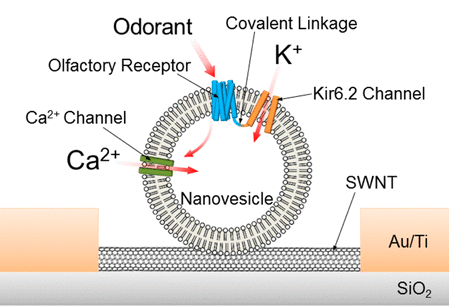
\includegraphics{figures/ch3/ion-channel-nanovesicle-lim2015.png}

}

}

\end{minipage}%
%
\begin{minipage}[t]{0.01\linewidth}

{\centering 

~

}

\end{minipage}%
%
\begin{minipage}[t]{0.03\linewidth}

{\centering 

\raisebox{-\height}{


\includegraphics{figures/(b).png}

}

}

\end{minipage}%
%
\begin{minipage}[t]{0.01\linewidth}

{\centering 

~

}

\end{minipage}%
%
\begin{minipage}[t]{0.45\linewidth}

{\centering 

\raisebox{-\height}{

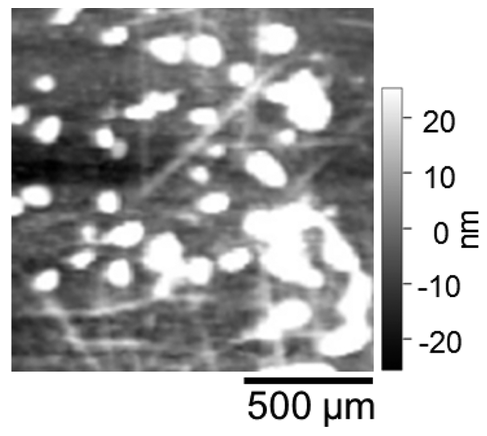
\includegraphics{figures/ch3/afm-nanovesicle-lim2015.png}

}

}

\end{minipage}%
%
\begin{minipage}[t]{0.01\linewidth}

{\centering 

~

}

\end{minipage}%
\newline
\begin{minipage}[t]{0.03\linewidth}

{\centering 

\raisebox{-\height}{


\includegraphics{figures/(c).png}

}

}

\end{minipage}%
%
\begin{minipage}[t]{0.01\linewidth}

{\centering 

~

}

\end{minipage}%
%
\begin{minipage}[t]{0.45\linewidth}

{\centering 

\raisebox{-\height}{

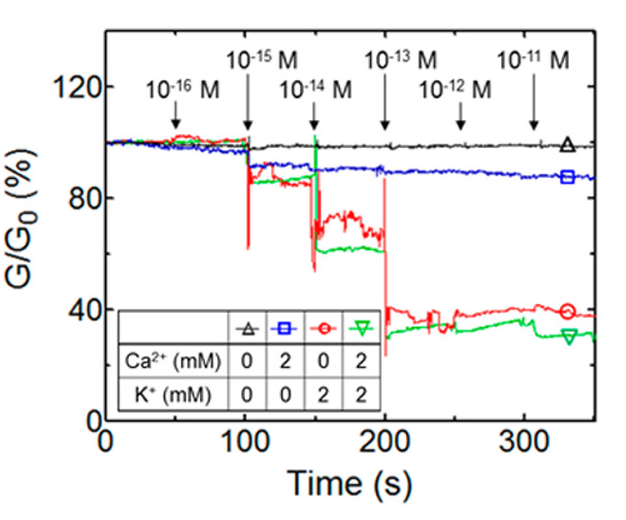
\includegraphics{figures/ch3/nanovesicle-amyl-butyrate-1-lim2015.png}

}

}

\end{minipage}%
%
\begin{minipage}[t]{0.01\linewidth}

{\centering 

~

}

\end{minipage}%
%
\begin{minipage}[t]{0.03\linewidth}

{\centering 

\raisebox{-\height}{

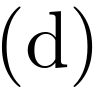
\includegraphics{figures/(d).png}

}

}

\end{minipage}%
%
\begin{minipage}[t]{0.01\linewidth}

{\centering 

~

}

\end{minipage}%
%
\begin{minipage}[t]{0.45\linewidth}

{\centering 

\raisebox{-\height}{

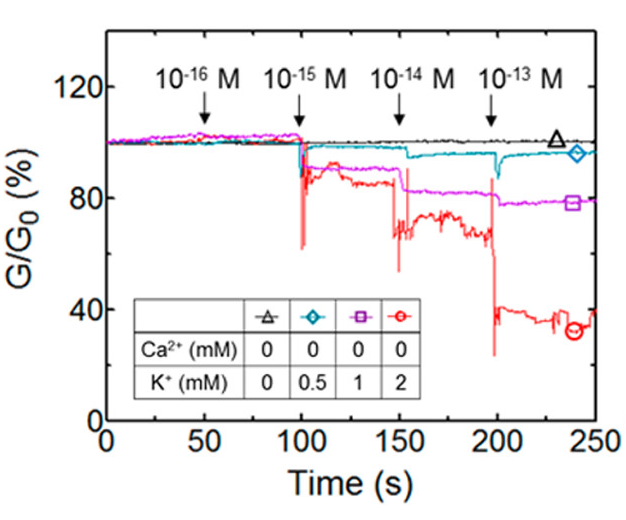
\includegraphics{figures/ch3/lim2015-potassium1.png}

}

}

\end{minipage}%
%
\begin{minipage}[t]{0.01\linewidth}

{\centering 

~

}

\end{minipage}%
\newline
\begin{minipage}[t]{0.03\linewidth}

{\centering 

\raisebox{-\height}{

\includegraphics{figures/(e).png}

}

}

\end{minipage}%
%
\begin{minipage}[t]{0.01\linewidth}

{\centering 

~

}

\end{minipage}%
%
\begin{minipage}[t]{0.45\linewidth}

{\centering 

\raisebox{-\height}{

\includegraphics{figures/ch3/nanovesicle-amyl-butyrate-2-lim2015.png}

}

}

\end{minipage}%
%
\begin{minipage}[t]{0.01\linewidth}

{\centering 

~

}

\end{minipage}%
%
\begin{minipage}[t]{0.03\linewidth}

{\centering 

\raisebox{-\height}{

\includegraphics{figures/(f).png}

}

}

\end{minipage}%
%
\begin{minipage}[t]{0.01\linewidth}

{\centering 

~

}

\end{minipage}%
%
\begin{minipage}[t]{0.45\linewidth}

{\centering 

\raisebox{-\height}{

\includegraphics{figures/ch3/lim2015-potassium2.png}

}

}

\end{minipage}%
%
\begin{minipage}[t]{0.01\linewidth}

{\centering 

~

}

\end{minipage}%

\caption[Schematics detailing the nanovesicle-based carbon nanotube
field-effect biosensor of Lim \emph{et
al.}]{\label{fig-lim-ion-channel}Schematics detailing the
nanovesicle-based carbon nanotube field-effect biosensor of Lim \emph{et
al.} (a) shows a schematic of the various signalling pathways present in
the sensor (not to scale), while (b) shows an atomic force microscope
image of the functionalised device. Real-time conductance changes
resulting from amyl butyrate additions are compared against relevant
controls in (c) and (d), while the dose-dependent response patterns to
amyl butyrate corresponding to (c) and (d) are shown in (e) and (f)
respectively. The key in (c)-(f) indicates the concentration of ions
available to flow through nanovesicle ion channels in each experimental
series. Reprinted with permission from \autocite{Lim2015}. Copyright
\(\copyright\) 2015 American Chemical Society.}

\end{figure}

\begin{figure}

\begin{minipage}[t]{0.03\linewidth}

{\centering 

\raisebox{-\height}{

\includegraphics{figures/(a).png}

}

}

\end{minipage}%
%
\begin{minipage}[t]{0.04\linewidth}

{\centering 

~

}

\end{minipage}%
%
\begin{minipage}[t]{0.90\linewidth}

{\centering 

\raisebox{-\height}{

\includegraphics{figures/ch3/kwon2015-OR-graphene.png}

}

}

\end{minipage}%
%
\begin{minipage}[t]{0.04\linewidth}

{\centering 

~

}

\end{minipage}%
\newline
\begin{minipage}[t]{0.03\linewidth}

{\centering 

\raisebox{-\height}{

\includegraphics{figures/(b).png}

}

}

\end{minipage}%
%
\begin{minipage}[t]{0.01\linewidth}

{\centering 

~

}

\end{minipage}%
%
\begin{minipage}[t]{0.45\linewidth}

{\centering 

\raisebox{-\height}{

\includegraphics{figures/ch3/kwon2015_transfer.png}

}

}

\end{minipage}%
%
\begin{minipage}[t]{0.01\linewidth}

{\centering 

~

}

\end{minipage}%
%
\begin{minipage}[t]{0.03\linewidth}

{\centering 

\raisebox{-\height}{

\includegraphics{figures/(c).png}

}

}

\end{minipage}%
%
\begin{minipage}[t]{0.01\linewidth}

{\centering 

~

}

\end{minipage}%
%
\begin{minipage}[t]{0.45\linewidth}

{\centering 

\raisebox{-\height}{

\includegraphics{figures/ch3/kwon2015-amyl-butyrate.png}

}

}

\end{minipage}%
%
\begin{minipage}[t]{0.01\linewidth}

{\centering 

~

}

\end{minipage}%
\newline
\begin{minipage}[t]{0.03\linewidth}

{\centering 

\raisebox{-\height}{

\includegraphics{figures/(d).png}

}

}

\end{minipage}%
%
\begin{minipage}[t]{0.01\linewidth}

{\centering 

~

}

\end{minipage}%
%
\begin{minipage}[t]{0.45\linewidth}

{\centering 

\raisebox{-\height}{

\includegraphics{figures/ch3/kwon2015-helional.png}

}

}

\end{minipage}%
%
\begin{minipage}[t]{0.01\linewidth}

{\centering 

~

}

\end{minipage}%
%
\begin{minipage}[t]{0.03\linewidth}

{\centering 

\raisebox{-\height}{

\includegraphics{figures/(e).png}

}

}

\end{minipage}%
%
\begin{minipage}[t]{0.01\linewidth}

{\centering 

~

}

\end{minipage}%
%
\begin{minipage}[t]{0.45\linewidth}

{\centering 

\raisebox{-\height}{

\includegraphics{figures/ch3/kwon2015-dose.png}

}

}

\end{minipage}%
%
\begin{minipage}[t]{0.01\linewidth}

{\centering 

~

}

\end{minipage}%

\caption[Schematics showing the odorant receptor-functionalised graphene
field-effect biosensor of Kwon \emph{et
al.}]{\label{fig-kwon-multiplexed}Schematics showing the odorant
receptor-functionalised graphene field-effect biosensor of Kwon \emph{et
al.} (a) shows the functionalisation of odorant receptors onto graphene
using non-covalently attached GA-modified DAN linker; (b) compares
transfer characteristics of the device with graphene only (GM), graphene
with DAN linker (GM/DAN), and after modification with one of two
different ORs (hOR2AG1, hOR3A1); (c) shows the real-time responses of
the liquid-gated hOR2AG1-modified transistor (sub-SB2) to various
concentrations of amyl butyrate (AB) analyte; (d) shows the real-time
responses of the hOR3A1-modified transistor (sub-SB3) to various
concentrations of helional (HE) analyte; and (e) shows the
dose-dependent response curve corresponding to the sub-SB2 and sub-SB3
sensors. Reprinted with permission from \autocite{Kwon2015}. Copyright
\(\copyright\) 2015 American Chemical Society.}

\end{figure}

\begin{figure}

\begin{minipage}[t]{0.03\linewidth}

{\centering 

\raisebox{-\height}{

\includegraphics{figures/(a).png}

}

}

\end{minipage}%
%
\begin{minipage}[t]{0.01\linewidth}

{\centering 

~

}

\end{minipage}%
%
\begin{minipage}[t]{0.45\linewidth}

{\centering 

\raisebox{-\height}{

\includegraphics{figures/ch3/yoo2022-micelle-cnt.png}

}

}

\end{minipage}%
%
\begin{minipage}[t]{0.01\linewidth}

{\centering 

~

}

\end{minipage}%
%
\begin{minipage}[t]{0.03\linewidth}

{\centering 

\raisebox{-\height}{

\includegraphics{figures/(b).png}

}

}

\end{minipage}%
%
\begin{minipage}[t]{0.01\linewidth}

{\centering 

~

}

\end{minipage}%
%
\begin{minipage}[t]{0.45\linewidth}

{\centering 

\raisebox{-\height}{

\includegraphics{figures/ch3/yoo2022-AFM.png}

}

}

\end{minipage}%
%
\begin{minipage}[t]{0.01\linewidth}

{\centering 

~

}

\end{minipage}%
\newline
\begin{minipage}[t]{0.03\linewidth}

{\centering 

\raisebox{-\height}{

\includegraphics{figures/(c).png}

}

}

\end{minipage}%
%
\begin{minipage}[t]{0.01\linewidth}

{\centering 

~

}

\end{minipage}%
%
\begin{minipage}[t]{0.45\linewidth}

{\centering 

\raisebox{-\height}{

\includegraphics{figures/ch3/yoo2022-TX.png}

}

}

\end{minipage}%
%
\begin{minipage}[t]{0.01\linewidth}

{\centering 

~

}

\end{minipage}%
%
\begin{minipage}[t]{0.03\linewidth}

{\centering 

\raisebox{-\height}{

\includegraphics{figures/(d).png}

}

}

\end{minipage}%
%
\begin{minipage}[t]{0.01\linewidth}

{\centering 

~

}

\end{minipage}%
%
\begin{minipage}[t]{0.45\linewidth}

{\centering 

\raisebox{-\height}{

\includegraphics{figures/ch3/yoo2022-DMMP.png}

}

}

\end{minipage}%
%
\begin{minipage}[t]{0.01\linewidth}

{\centering 

~

}

\end{minipage}%
\newline
\begin{minipage}[t]{0.03\linewidth}

{\centering 

\raisebox{-\height}{

\includegraphics{figures/(e).png}

}

}

\end{minipage}%
%
\begin{minipage}[t]{0.01\linewidth}

{\centering 

~

}

\end{minipage}%
%
\begin{minipage}[t]{0.45\linewidth}

{\centering 

\raisebox{-\height}{

\includegraphics{figures/ch3/yoo2022-DMMP-2.png}

}

}

\end{minipage}%
%
\begin{minipage}[t]{0.01\linewidth}

{\centering 

~

}

\end{minipage}%
%
\begin{minipage}[t]{0.03\linewidth}

{\centering 

\raisebox{-\height}{

\includegraphics{figures/(f).png}

}

}

\end{minipage}%
%
\begin{minipage}[t]{0.01\linewidth}

{\centering 

~

}

\end{minipage}%
%
\begin{minipage}[t]{0.45\linewidth}

{\centering 

\raisebox{-\height}{

\includegraphics{figures/ch3/yoo2022-DMMP-3.png}

}

}

\end{minipage}%
%
\begin{minipage}[t]{0.01\linewidth}

{\centering 

~

}

\end{minipage}%

\caption[Schematics of the micelle-based carbon nanotube field-effect
transistor of Yoo \emph{et al.}]{\label{fig-yoo-micelle}Schematics of
the micelle-based carbon nanotube field-effect transistor of Yoo
\emph{et al.} (a) shows the functionalisation of detergent micelles onto
the carbon nanotube network channel; (b) shows the same height profile
across an atomic force microscope image of the carbon nanotube network
before and after functionalisation with micelles using PBASE; (c) shows
the liquid-gated transfer characteristic of a device channel before and
after functionalisation with PBASE and micelles; (d) shows real-time
responses of the functionalised, liquid-gated channel to additions of
dimethyl methylphosphonate (DMMP) analyte; (e) shows the dose-dependent
response curve to DMMP; and (f) shows a control series demonstrating the
selective behaviour of the sensor (EB is ethyl butyrate, AB is amyl
butyrate). Adapted with permission from \autocite{Yoo2022}. Copyright
\(\copyright\) 2022 Elsevier.}

\end{figure}

Vertebrate odorant receptors have previously been coupled with
nanovesicle ion channels for selective analyte detection
\autocite{Lim2015,Dung2018}. Lim \emph{et al.} synthesised nanovesicles
featuring the human odorant receptor hOR2AG1, covalently coupled with a
potassium ion channel and placed alongside an endogenous calcium ion
channel. This configuration is shown in Figure~\ref{fig-lim-ion-channel}
(a). These nanovesicles were attached to the carbon nanotube network of
a thin-film device via charge-charge interaction with poly-D-lysine,
demonstrated with the atomic force microscope image in
Figure~\ref{fig-lim-ion-channel} (b). Binding of amyl butyrate to
hOR2AG1 causes the OR to change conformation, opening the coupled
potassium ion channel and causing ions to flow into the nanovesicle,
resulting in transistor channel gating. The real-time signal responses
associated with channel gating due to ion flow are shown in
Figure~\ref{fig-lim-ion-channel} (c)-(f). Intracellular signalling by
the odorant receptors means that target binding also activates the
calcium ion channel, and so the presence of calcium ions is sufficient
for a sensing response. In all electrolytes used to obtain a signal
response, ions are present in high concentrations relative to analyte,
ensuring ions are readily available for signalling processes. Without
either potassium or calcium ions present, ion inflow cannot occur, so no
conductance change is observed \autocite{Lim2015}.

Odorant receptors can also be expressed in the native cell membrane and
attached directly to the biosensor channel. Here, the changes in odorant
receptor conformation that result from analyte binding cause affects the
distance between charges on the odorant receptor and the transducer
channel, gating the channel \autocite{Kwon2015,Dung2018}. Kwon \emph{et
al.} functionalised graphene field-effect transistors with human odorant
receptors hOR2AG1 and hOR3A1 using non-covalently attached
1,5-diaminonaphthalene (DAN) modified with glutaraldehyde (GA) as a
linker, as shown in Figure~\ref{fig-kwon-multiplexed} (a). The odorant
receptors attach to the GA-modified DAN via a Schiff-base reaction
\autocite{Bhatt2021}. OR attachment was demonstrated by SEM imaging as
well as a significant change in device resistance, shown in
Figure~\ref{fig-kwon-multiplexed} (b). Both hOR2AG1 and hOR3A1 showed
real-time responses to their corresponding target analyte at
sub-femtomolar concentrations, as shown in
Figure~\ref{fig-kwon-multiplexed} (c) and
Figure~\ref{fig-kwon-multiplexed} (d) respectively. No responses were
seen from linker-modified graphene to the same analyte additions. The
dose-dependent response curve of both these odorant receptor sensors is
shown in Figure~\ref{fig-kwon-multiplexed} (e). As in
Figure~\ref{fig-lim-ion-channel} (d), the response behaviour follows a
curve which can be described using a Langmuir surface adsorption
isotherm, with saturation behaviour observed with picomolar additions.

Biosensors have also been produced where odorant receptors are held in a
detergent micelle format instead of the native cell membrane. The
mechanism behind sensing is the same as for odorant receptors in the
cell membrane, where a conformational change in the odorant receptors
leads to channel gating \autocite{Dung2018,Yoo2022}. Yoo \emph{et al.}
functionalised random-network CNT FETs with detergent micelles which
contained human odorant receptor hOR2T7. PBASE was used as the linker
molecule, which attaches to the odorant receptor via its amine group and
non-covalently tethers it to the transducer, illustrated in
Figure~\ref{fig-yoo-micelle} (a). Successful immobilisation was
demonstrated by a raised atomic force microscope height profile after
receptor attachment (Figure~\ref{fig-yoo-micelle} (b)) and an on-current
drop in the liquid-gated transfer characteristics of the device
(Figure~\ref{fig-yoo-micelle} (c)). The sensor showed sharp real-time
responses to the addition of DMMP concentrations, as seen in
Figure~\ref{fig-yoo-micelle} (d). The dose dependence curve for DMMP
responses is shown in in Figure~\ref{fig-yoo-micelle} (e), again showing
a Langmuir-type response curve to successive DMMP additions. Various
analytes with a similar scent to DMMP were added at high concentrations
to the liquid-gate, shown in Figure~\ref{fig-yoo-micelle} (f). No
response was seen to any these additions, demonstrating the selectivity
of the sensor.

\begin{figure}

\begin{minipage}[t]{0.03\linewidth}

{\centering 

\raisebox{-\height}{

\includegraphics{figures/(a).png}

}

}

\end{minipage}%
%
\begin{minipage}[t]{0.01\linewidth}

{\centering 

~

}

\end{minipage}%
%
\begin{minipage}[t]{0.40\linewidth}

{\centering 

\raisebox{-\height}{

\includegraphics{figures/ch3/afm-nanodisc-goldsmith.png}

}

}

\end{minipage}%
%
\begin{minipage}[t]{0.01\linewidth}

{\centering 

~

}

\end{minipage}%
%
\begin{minipage}[t]{0.03\linewidth}

{\centering 

\raisebox{-\height}{

\includegraphics{figures/(b).png}

}

}

\end{minipage}%
%
\begin{minipage}[t]{0.01\linewidth}

{\centering 

~

}

\end{minipage}%
%
\begin{minipage}[t]{0.50\linewidth}

{\centering 

\raisebox{-\height}{

\includegraphics{figures/ch3/eugenol-goldsmith.png}

}

}

\end{minipage}%
%
\begin{minipage}[t]{0.01\linewidth}

{\centering 

~

}

\end{minipage}%

\caption[Functionalisation and sensing behaviour of the nanodisc-based
carbon nanotube field-effect transistor of Goldsmith \emph{et
al.}]{\label{fig-eugenol-responses}The functionalisation of mOR174-9
nanodiscs onto single-CNT field effect transistor vapour sensing use is
demonstrated with an atomic force microscope image in (a), while (b)
shows real-time responses of the sensor to 2 ppm eugenol vapour. The
response to eugenol on day 69 (red triangles) indicates that the device
retains the ability to respond to eugenol 10 weeks after
functionalisation. Reprinted with permission from
\autocite{Goldsmith2011}. Copyright \(\copyright\) 2011 American
Chemical Society.}

\end{figure}

In the first study of its kind, Goldsmith \emph{et al.} demonstrated
that a single-CNT device functionalised with mOR174-9 odorant receptors
in either a micelle or nanodisc format could be used as a vapour-phase
biosensor. Micelle immobilisation was confirmed using atomic force
microscopy, as shown in Figure~\ref{fig-eugenol-responses} (a). The mOR
CNT FETs were exposed to nitrogen flow at 50\% relative humidity. The
conductance across the channel was measured while a specific
concentration of the positive ligand eugenol was added to the constant
flow for 100 s, then removed from the flow for 100 s. This cycle was
repeated five times. Figure~\ref{fig-eugenol-responses} (b) shows that a
\(\sim\) 9\% increase in current was observed during each cycle of
exposure to eugenol. The device still responded to eugenol cycles after
69 days of storage in 25\% (v/v) ethanol at 4 °C. This persistent
activity may result from the long-lived nanodisc format used
\autocite{Goldsmith2011}. As far as the author knows, no study currently
exists which investigates whether this behaviour can be replicated for
the behaviourally-distinct insect odorant receptor devices. It is not
clear that the vertebrate odorant receptors used here can simply be
substituted for iORs for vapour-phase sensing.

\hypertarget{sec-insect-OR-biosensors}{%
\section{Insect Odorant Receptor Field-Effect Transistor
Biosensors}\label{sec-insect-OR-biosensors}}

\hypertarget{insect-odorant-receptors}{%
\subsection{Insect Odorant Receptors}\label{insect-odorant-receptors}}

Insect odorant (or olfactory) receptors (iORs) are a diverse range of
odorant-sensitive seven-transmembrane proteins located in the dendrite
cells of insect sensory hairs, known as sensilla
\autocite{Clyne1999,Carraher2015,Brito2016,Wicher2021}. When volatile
compounds enter the sensilla, they are carried by odorant binding
proteins (OBPs) through an aqueous environment to the dendrite cells
\autocite{Carraher2015,Brito2016,Wicher2021}. These cells possess a
insect-specific set of ``tuning'' iORs alongside a generic co-receptor
known as ``ORCO'' (Odorant Receptor Co-Receptor)
\autocite{Carraher2015,Butterwick2018,Khadka2019,Wicher2021}. The ORCO
co-receptor is insensitive to target compounds (aside from synthetic
compounds like VUAA1). Instead, it couples with the tuning iOR to form a
non-selective, permeable ion channel
\autocite{Butterwick2018,Wicher2021}. When a compound binds to a tuning
iOR, the ion channel opens to allow cations to travel across the cell
membrane, activating intracellular signalling
\autocite{Smart2008,Wicher2008,Sato2008,Carraher2015,Brito2016,Butterwick2018,Wicher2021}.
The combination of resulting OR signals is sent to the insect brain for
interpretation as an odor \autocite{Hallem2004,Carraher2015,Wicher2021}.
The tuning iORs respond to (or are inhibited by) a huge variety of odors
\autocite{Munch2016}. The non-trivial binding behaviour of iORs with
analyte means artificial neural network processing may be required for
accurate readouts from a self-contained, lab-on-a-chip iOR biosensor
\autocite{Bachtiar2016}.

\begin{figure}

{\centering \includegraphics[width=0.65\textwidth,height=\textheight]{figures/ch3/OR_diagram.png}

}

\caption[The tuning OR and odorant receptor coreceptor (ORCO) on the
native cell membrane, with C-terminus and N-terminus
indicated.]{\label{fig-iOR-membrane}The tuning OR and odorant receptor
coreceptor (ORCO) on the native cell membrane, with C-terminus and
N-terminus indicated. The red arrow indicates the location of ion
transport across the membrane.}

\end{figure}

Vertebrate odorant receptor proteins are terminated with an amine group
outside the cell membrane, known as the N-terminus, and terminated with
a carboxyl group inside the cell membrane, known as the C-terminus.
Initially, iORs were thought to be similar in structure to vertebrate
GPCRs \autocite{Clyne1999}, but is now known that iORs have a completely
different topology and mechanism, despite also being a
seven-transmembrane protein. The terminus configuration is inverted: the
C-terminus of the iOR is extracellular, and the N-terminus is
intracellular
\autocite{Smart2008,Glatz2011,Carraher2015,Brito2016,Wicher2021}.
Furthermore, there is no sequence similarity between iORs and GPCRs.
Evolutionarily, insect odorant receptors are thought to be closely
related to insect gustatory receptors (GRs), while they bear no relation
to GPCRs \autocite{Glatz2011,Carraher2015,Wicher2021}. However, despite
iORs not being GPCRs, some interaction between the iOR complex and the
G-protein of the olfactory cell plays a role in odor detection \emph{in
vivo} \autocite{Wicher2008,Wicher2021}. The \emph{in vivo} configuration
of the odorant receptor on the cell membrane, showing the terminus
configuration and location of ORCO ion channel, is illustrated in
Figure~\ref{fig-iOR-membrane}. By testing sensors which incorporate
insect odorant receptors, new information may emerge which helps us to
better understand their atypical structure.

\hypertarget{sensor-functionalisation}{%
\subsection{Sensor Functionalisation}\label{sensor-functionalisation}}

\begin{figure}

\begin{minipage}[t]{0.03\linewidth}

{\centering 

\raisebox{-\height}{

\includegraphics{figures/(a).png}

}

}

\end{minipage}%
%
\begin{minipage}[t]{0.01\linewidth}

{\centering 

~

}

\end{minipage}%
%
\begin{minipage}[t]{0.45\linewidth}

{\centering 

\raisebox{-\height}{

\includegraphics{figures/ch3/pristine_graphene_murugathas.png}

}

}

\end{minipage}%
%
\begin{minipage}[t]{0.01\linewidth}

{\centering 

~

}

\end{minipage}%
%
\begin{minipage}[t]{0.03\linewidth}

{\centering 

\raisebox{-\height}{

\includegraphics{figures/(b).png}

}

}

\end{minipage}%
%
\begin{minipage}[t]{0.01\linewidth}

{\centering 

~

}

\end{minipage}%
%
\begin{minipage}[t]{0.45\linewidth}

{\centering 

\raisebox{-\height}{

\includegraphics{figures/ch3/OR22a_graphene_murugathas.png}

}

}

\end{minipage}%
%
\begin{minipage}[t]{0.01\linewidth}

{\centering 

~

}

\end{minipage}%
\newline
\begin{minipage}[t]{0.03\linewidth}

{\centering 

\raisebox{-\height}{

\includegraphics{figures/(c).png}

}

}

\end{minipage}%
%
\begin{minipage}[t]{0.01\linewidth}

{\centering 

~

}

\end{minipage}%
%
\begin{minipage}[t]{0.45\linewidth}

{\centering 

\raisebox{-\height}{

\includegraphics{figures/ch3/pristine_CNT_murugathas.png}

}

}

\end{minipage}%
%
\begin{minipage}[t]{0.01\linewidth}

{\centering 

~

}

\end{minipage}%
%
\begin{minipage}[t]{0.03\linewidth}

{\centering 

\raisebox{-\height}{

\includegraphics{figures/(d).png}

}

}

\end{minipage}%
%
\begin{minipage}[t]{0.01\linewidth}

{\centering 

~

}

\end{minipage}%
%
\begin{minipage}[t]{0.45\linewidth}

{\centering 

\raisebox{-\height}{

\includegraphics{figures/ch3/OR22a_CNT_murugathas.png}

}

}

\end{minipage}%
%
\begin{minipage}[t]{0.01\linewidth}

{\centering 

~

}

\end{minipage}%

\caption[Atomic force microscope images of pristine and
nanodisc-functionalised
thin-films.]{\label{fig-functionalisation-AFM-literature}Atomic force
microscope images of (a) a pristine graphene monolayer, (b) a OR22a
nanodisc-functionalised graphene monolayer, (c) a pristine carbon
nanotube network, and (d) an OR22a nanodisc-functionalised carbon
nanotube network. Reprinted with permission from
\autocite{Murugathas2019a,Murugathas2020}. Copyright \(\copyright\)
2019, 2020 American Chemical Society.}

\end{figure}

Murugathas \emph{et al.} attached a variety of insect odorant receptors
to carbon nanotubes and graphene field-effect transistors using a
nanodisc format. Figure~\ref{fig-functionalisation-AFM-literature} shows
atomic force microscope images of a graphene monolayer before and after
immobilisation of OR22a nanodiscs with PBASE linker in (a) and (b)
respectively, while atomic force microscope images of a randomly
deposited carbon nanotube network before and after OR22a nanodisc
immobilisation with PBASE are shown in (c) and (d) respectively.
Features are seen across the surface of the post-functionalisation image
which are tens of nanometers in height. On the nanotube network, these
features are seen directly next to nanotube bundles, indicating
selective attachment to the nanotubes over the SiO\(_2\) substrate. As
nanodiscs are only 10-20 nm in height, it appears that these features
are large agglomerates of nanodiscs
\autocite{Nath2007,Bayburt2010,Murugathas2019a,Murugathas2020}. As seen
previously for a carbon nanotube network FET in
Section~\ref{sec-odorant-receptors-biosensors}, functionalisation occurs
by non-covalent attachment of PBASE to the channel, and covalent
attachment of the PBASE linker to the odorant receptor amine group. The
nanodisc membrane also possesses amine residues \autocite{Bayburt2010},
so in some cases immobilisation may be directly between the PBASE linker
and nanodisc membrane.

\begin{figure}

\begin{minipage}[t]{0.03\linewidth}

{\centering 

\raisebox{-\height}{

\includegraphics{figures/(a).png}

}

}

\end{minipage}%
%
\begin{minipage}[t]{0.01\linewidth}

{\centering 

~

}

\end{minipage}%
%
\begin{minipage}[t]{0.45\linewidth}

{\centering 

\raisebox{-\height}{

\includegraphics{figures/ch3/OR22a_ND_GFET.png}

}

}

\end{minipage}%
%
\begin{minipage}[t]{0.01\linewidth}

{\centering 

~

}

\end{minipage}%
%
\begin{minipage}[t]{0.03\linewidth}

{\centering 

\raisebox{-\height}{

\includegraphics{figures/(b).png}

}

}

\end{minipage}%
%
\begin{minipage}[t]{0.01\linewidth}

{\centering 

~

}

\end{minipage}%
%
\begin{minipage}[t]{0.45\linewidth}

{\centering 

\raisebox{-\height}{

\includegraphics{figures/ch3/OR22a_ND_CNTFET.png}

}

}

\end{minipage}%
%
\begin{minipage}[t]{0.01\linewidth}

{\centering 

~

}

\end{minipage}%
\newline
\begin{minipage}[t]{0.03\linewidth}

{\centering 

\raisebox{-\height}{

\includegraphics{figures/(c).png}

}

}

\end{minipage}%
%
\begin{minipage}[t]{0.01\linewidth}

{\centering 

~

}

\end{minipage}%
%
\begin{minipage}[t]{0.45\linewidth}

{\centering 

\raisebox{-\height}{

\includegraphics{figures/ch3/Empty_ND_GFET.png}

}

}

\end{minipage}%
%
\begin{minipage}[t]{0.01\linewidth}

{\centering 

~

}

\end{minipage}%
%
\begin{minipage}[t]{0.03\linewidth}

{\centering 

\raisebox{-\height}{

\includegraphics{figures/(d).png}

}

}

\end{minipage}%
%
\begin{minipage}[t]{0.01\linewidth}

{\centering 

~

}

\end{minipage}%
%
\begin{minipage}[t]{0.45\linewidth}

{\centering 

\raisebox{-\height}{

\includegraphics{figures/ch3/Empty_ND_CNTFET.png}

}

}

\end{minipage}%
%
\begin{minipage}[t]{0.01\linewidth}

{\centering 

~

}

\end{minipage}%

\caption[Transfer characteristic curves of graphene and carbon nanotube
network field-effect transistors before and after OR22a
functionalisation.]{\label{fig-functionalisation-literature}Transfer
characteristic curves before and after functionalisation of (a) an OR22a
nanodisc-functionalised graphene field-effect transistor, (b) an OR22a
nanodisc-functionalised CNT network FET, (c) an empty
nanodisc-functionalised graphene FET and (d) an empty
nanodisc-functionalised CNT network FET. Reproduced with permission from
\autocite{Murugathas2019a,Murugathas2020}.}

\end{figure}

Functionalisation of a FET device channel with iORs significantly alters
the transfer characteristics of that channel. Murugathas \emph{et al.}
found that successful functionalisation of a CNT FET device with iORs
would typically increase the device on-current, increase its on-off
ratio and cause a significant negative shift in threshold voltage, as
shown in Figure~\ref{fig-functionalisation-literature} (a)
\autocite{Murugathas2019a}. Meanwhile, successful functionalisation of a
graphene device with iORs would typically dramatically decrease the
device on-current and cause a negative shift in Dirac voltage, as seen
in Figure~\ref{fig-functionalisation-literature} (b)
\autocite{Murugathas2020}. These changes are not simply the result of
linker attachment to the channel surface \autocite{Murugathas2019a}. It
is thought that the negative shift of both threshold and Dirac voltages
are caused by the N-terminus amine groups on the odorant receptors or
amine groups on the nanodisc membrane scaffold proteins donating
electrons to the device channel, which has a similar effect to doping
the channel with impurities
\autocite{Bradley2004,Murugathas2019a,Murugathas2020}. Note that very
similar changes occur when functionalising with empty nanodiscs which
contain no odorant receptors, shown in
Figure~\ref{fig-functionalisation-literature} (c) and
Figure~\ref{fig-functionalisation-literature} (d). Unless the odorant
receptors attach preferentially to the network over nanodiscs, it
appears the gating effect is predominantly due to the large-scale
attachment of nanodisc membranes.

\hypertarget{sensing-behaviour-1}{%
\subsection{Sensing Behaviour}\label{sensing-behaviour-1}}

\begin{figure}

\begin{minipage}[t]{0.03\linewidth}

{\centering 

\raisebox{-\height}{

\includegraphics{figures/(a).png}

}

}

\end{minipage}%
%
\begin{minipage}[t]{0.01\linewidth}

{\centering 

~

}

\end{minipage}%
%
\begin{minipage}[t]{0.45\linewidth}

{\centering 

\raisebox{-\height}{

\includegraphics{figures/ch3/OR22a_realtime_normalised_GFET_1.png}

}

}

\end{minipage}%
%
\begin{minipage}[t]{0.01\linewidth}

{\centering 

~

}

\end{minipage}%
%
\begin{minipage}[t]{0.03\linewidth}

{\centering 

\raisebox{-\height}{

\includegraphics{figures/(b).png}

}

}

\end{minipage}%
%
\begin{minipage}[t]{0.01\linewidth}

{\centering 

~

}

\end{minipage}%
%
\begin{minipage}[t]{0.45\linewidth}

{\centering 

\raisebox{-\height}{

\includegraphics{figures/ch3/OR22a_realtime_normalised_CNTFET_1.png}

}

}

\end{minipage}%
%
\begin{minipage}[t]{0.01\linewidth}

{\centering 

~

}

\end{minipage}%
\newline
\begin{minipage}[t]{0.03\linewidth}

{\centering 

\raisebox{-\height}{

\includegraphics{figures/(c).png}

}

}

\end{minipage}%
%
\begin{minipage}[t]{0.01\linewidth}

{\centering 

~

}

\end{minipage}%
%
\begin{minipage}[t]{0.45\linewidth}

{\centering 

\raisebox{-\height}{

\includegraphics{figures/ch3/OR22a_realtime_normalised_GFET_2.png}

}

}

\end{minipage}%
%
\begin{minipage}[t]{0.01\linewidth}

{\centering 

~

}

\end{minipage}%
%
\begin{minipage}[t]{0.03\linewidth}

{\centering 

\raisebox{-\height}{

\includegraphics{figures/(d).png}

}

}

\end{minipage}%
%
\begin{minipage}[t]{0.01\linewidth}

{\centering 

~

}

\end{minipage}%
%
\begin{minipage}[t]{0.45\linewidth}

{\centering 

\raisebox{-\height}{

\includegraphics{figures/ch3/OR22a_realtime_normalised_CNTFET_2.png}

}

}

\end{minipage}%
%
\begin{minipage}[t]{0.01\linewidth}

{\centering 

~

}

\end{minipage}%

\caption[Real-time sensing behaviour of graphene and carbon nanotube
network field-effect transistors before and after OR22a
functionalisation.]{\label{fig-iOR-sensing-literature}Real-time
responses to concentrations of methyl hexanoate in \(1 \times\)
phosphate buffer saline (PBS) with 1\% v/v DMSO by (a) an OR22a
nanodisc-functionalised graphene field-effect transistor and (b) an
OR22a nanodisc-functionalised CNT network FET, alongside the normalised
signal response curves corresponding to (c) graphene FETs and (d) carbon
nanotube network FETs. The response curves show the cumulative responses
of OR22a-functionalised devices to both the positive ligand methyl
hexanoate (green) and negative ligand \emph{trans}-2-hexan-1-al (black).
They also show the cumulative response of a empty nanodisc
functionalised device to methyl hexanoate (purple). Reproduced with
permission from \autocite{Murugathas2019a,Murugathas2020}.}

\end{figure}

Figure~\ref{fig-iOR-sensing-literature} (a) and (b) show the respective
responses of the OR22a-functionalised graphene FET and CNT FET to
various concentrations of methyl hexanoate in real-time. This result
demonstrates that iOR-FETs are sensitive down to the femtomolar scale in
an aqueous environment. Figure~\ref{fig-iOR-sensing-literature} (c) and
(d) compare the dose dependent responses to methyl hexanoate from
multiple OR22a-functionalised devices to that of relevant controls. It
was verified that the OR22a-functionalised devices would not respond to
\emph{trans}-2-hexan-1-al, the negative ligand for OR22a; it was also
verified that empty nanodiscs would not respond non-selectively to the
positive ligand \autocite{Murugathas2019a,Murugathas2020}. It is notable
that unlike iORs \emph{in vivo}, ORCO does not appear to be required for
the bioelectronic nose to function
\autocite{Murugathas2019a,Murugathas2020,Khadka2019,Cheema2021}.
Furthermore, G-protein signaling pathways are not required
\autocite{Sato2014}. It has been proposed that the signal response
results from the positive ligand binding to the iOR protein, causing a
change in conformation, the same mechanism underpinning the behaviour of
many of the vertebrate odorant receptor sensors seen in
Section~\ref{sec-odorant-receptors-biosensors}. Cheema \emph{et al.}
used neutron reflectometry to demonstrate that OR22a nanodiscs undergo a
1 nm height change after ethyl hexanoate exposure, likely resulting from
a structural change \autocite{Cheema2021}.

This change most likely affects the channel in one of two ways. The
first involves transfer of charge from the iOR to the channel, reducing
I\(_{d}\) and causing a negative threshold voltage (or Dirac point)
shift. Another could be a more indirect electrostatic gating effect from
movement of charge within the Debye screening length of the channel. The
Debye length of \(1 \times\) PBS buffer is typically much shorter than
the height of a single nanodisc \autocite{Murugathas2019a}. However, if
structural changes in the iOR were primarily occurring at its base, it
is still possible that the electrostatic gating could be the primary
sensing mechanism. From further development and examination of iOR-based
biosensors, new insights into the mechanisms underlying the nanodisc
signal transduction may emerge \autocite{Glatz2011}. As discussed here,
the literature has primarily focused on the operation of iOR carbon
nanotube and graphene FET biosensors in an aqueous environment
\autocite{Murugathas2019a,Murugathas2020}. It is as yet unknown whether
insect odorant receptors can operate in a vapour-phase environment, but
this possibility is explored in this thesis.

\hypertarget{sec-non-specific-binding}{%
\section{Non-Specific Binding}\label{sec-non-specific-binding}}

Non-specific binding (NSB) refers to any attachment within the sensing
environment not related to the specific analyte of interest
\autocite{Lichtenberg2019,Shkodra2021}. Non-specific binding is
particularly significant for protein-functionalised devices. Proteins
may be spontaneously adsorbed onto carbon nanotube or graphene surfaces
during functionalisation in a manner which is not linker-mediated
\autocite{Bradley2004,Star2003a,Chen2004}. Non-covalently bound proteins
may detach and reattach to available surfaces in a non-specific manner
when exposed to a high ionic strength electrolyte post-functionalisation
\autocite{Dung2018}. Non-specific binding may also result from
protein-protein interactions, misoriented attachment of proteins,
attachment to a sticky substrate \autocite{Chen2004,Lichtenberg2019}. It
can also result from electrostatic binding to any charged surface
present, such as the gold electrodes \autocite{Garcia-Aljaro2010} or
Ag/AgCl reference electrode
\autocite{Chen2004,Minot2007,Lichtenberg2019}. Liquid-gated graphene and
carbon nanotube devices are highly sensitive to the approach of charge
within the Debye length of the device channel, and so non-specific
adsorption can lead to spurious signals during sensing
\autocite{Star2003a,Chen2004,Lichtenberg2019,Shkodra2021}. A variety of
measures can be taken to prevent NSB from occurring. Once bioreceptors
have been attached to the channel, remaining exposed carbon nanotubes
can be passivated with chemical coatings such as Tween-20
\autocite{Chen2004}, PEG
\autocite{Star2003a,Lee2012b,Gao2016,Filipiak2018}, and ethanolamine
\autocite{Maehashi2007,Das2011}.

\hypertarget{summary-1}{%
\section{Summary}\label{summary-1}}

Odorant receptors can be used to fabricate highly sensitive and
selective biosensors using carbon nanotube and graphene field-effect
transistors as the transducer element. Both vertebrate and insect
odorant receptors are seven-transmembrane proteins, but each has a
different sequence and have inverted terminus positions relative to the
cell membrane wall \emph{in vivo}. Insect odorant receptor detection
\emph{in vivo} differs significantly from vertebrate OR detection, with
an ORCO-mediated ion channel involved. ORs can be held in the native
cell membrane for sensor applications, but artificial lipid bilayer
formats such as micelles, nanovesicles or nanodiscs are generally
preferred due to their enhanced stability. Mammalian odorant receptors
have been thoroughly explored in carbon nanotube and graphene
field-effect transistor sensing applications, with both non-covalent and
covalent functionalisation mechanisms used to create sensors which
detect analyte at sub-femtomolar concentrations. The mechanisms behind
sensing rely on transistor gating either due to ion flow into a
nanovesicle format, or a conformational change in the odorant receptor.
Covalently-attached mammalian odorant receptors have also been used for
vapour-phase detection with a single carbon nanotube field-effect
transistor device at concentrations down to \(\sim\) 7 ppb by Goldsmith
\emph{et al.}

Femtomolar detection of analyte has also been achieved with an insect
odorant receptor functionalised device. However, the exact mechanism
behind detection is unclear, as the presence of ORCO is not required for
successful sensor behaviour. It is possible that the mechanism results
from a change in conformation of the odorant receptor, similar to the
mammalian odorant receptor. Due to the possible difference in mechanism
between mammalian odorant receptor detection and insect odorant receptor
detection, it is not clear that vapour-phase detection can be achieved
by simply reproducing the work of Goldsmith \emph{et al.} using insect
odorant receptors. Chapter~\ref{sec-noncovalent-functionalisation} looks
further at various non-covalent functionalisation approaches for the
creation of a insect odorant receptor-based field-effect transistor
biosensor, while Chapter~\ref{sec-biosensing-iORs} tests sensor
behaviour in both aqueous and vapour-phase environments.

\bookmarksetup{startatroot}

\hypertarget{sec-fabrication}{%
\chapter{Fabrication and Characterisation of Thin-Film
Transistors}\label{sec-fabrication}}

\hypertarget{introduction-2}{%
\section{Introduction}\label{introduction-2}}

This chapter discusses the fabrication processes for both carbon
nanotube network and graphene thin-film transistors (TFTs). Experimental
optimisation of the transducer element is critical for biosensor work,
and large numbers of transducers were required for testing various
biosensor functionalisation processes. Therefore, these processes were
developed to rapidly fabricate devices with reproducible device
characteristics appropriate for biosensing work. Also outlined in this
chapter are the characterisation techniques taken to test the quality
and reproducibility of these fabrication processes.

The nitrogen (\(\geq\) 99.99\%) and oxygen (99.7\%) used in fabrication
work was supplied by BOC Limited New Zealand. All acetone and
isopropanol used for wafer/device processing had a minimum 99.9\% purity
(HPLC grade). Deionised (DI) water was taken from a
Synergy\(^\circledR\) UV Water Purification System. The DI water had a
measured conductivity of \((1.4\pm0.1)\textrm{ } \textrm{µS cm}^{-1}\),
compared to tap water with a measured conductivity of
\((7.8\pm0.2)\textrm{ } \textrm{µS cm}^{-1}\).

\hypertarget{sec-photolithography}{%
\section{Photolithography for Fabrication of Thin-Film
Transistors}\label{sec-photolithography}}

\hypertarget{general-overview}{%
\subsection{General Overview}\label{general-overview}}

This section details some of the standard photolithography procedures
used in the quarter wafer processing detailed in
Section~\ref{sec-qw-processing}. Photoresists, also referred to here as
``resists'', are UV light-sensitive polymeric resins used for
photolithography. ``Positive'' resists are made soluble in alkalines by
UV light exposure, meaning exposed areas are removed in the development
process. Conversely, ``negative'' resists are cross-linked by exposure
and a post-exposure bake step. The unexposed areas of the negative
resist are then removed in the development process
\autocite{Microchemicals1}. Both positive and negative resists are used
in this thesis. The processes for each type of resist are shown in
Figure~\ref{fig-photolithography-profiles} (a). The specific photoresist
selected for photolithography depends on the specific use case. The
types used in this thesis are positive and negative AZ\(^\circledR\)
photoresists (AZ\(^\circledR\) 1518, Microchemicals GmbH;
AZ\(^\circledR\) nLOF 2020, Microchemicals GmbH) and SU8 (SU8-2150,
Kayaku Advanced Materials, formerly Microchem). The AZ\(^\circledR\)
resists used have a minimum film thickness of
\(1.5\textrm{ } \textrm{µm}\) \autocite{Microchemicals1}, while the
SU8-2150 has a minimum film thickness of \(0.5\textrm{ } \textrm{µm}\)
\autocite{Kayaku}.

\begin{figure}

\begin{minipage}[t]{0.03\linewidth}

{\centering 

\raisebox{-\height}{

\includegraphics{figures/(a).png}

}

}

\end{minipage}%
%
\begin{minipage}[t]{0.01\linewidth}

{\centering 

~

}

\end{minipage}%
%
\begin{minipage}[t]{0.95\linewidth}

{\centering 

\raisebox{-\height}{

\includegraphics{figures/ch4/positive-negative-photolithography.png}

}

}

\end{minipage}%
%
\begin{minipage}[t]{0.01\linewidth}

{\centering 

~

}

\end{minipage}%
\newline
\begin{minipage}[t]{0.03\linewidth}

{\centering 

\raisebox{-\height}{

\includegraphics{figures/(b).png}

}

}

\end{minipage}%
%
\begin{minipage}[t]{0.01\linewidth}

{\centering 

~

}

\end{minipage}%
%
\begin{minipage}[t]{0.45\linewidth}

{\centering 

\raisebox{-\height}{

\includegraphics{figures/ch4/overcut-profile.png}

}

}

\end{minipage}%
%
\begin{minipage}[t]{0.01\linewidth}

{\centering 

~

}

\end{minipage}%
%
\begin{minipage}[t]{0.03\linewidth}

{\centering 

\raisebox{-\height}{

\includegraphics{figures/(c).png}

}

}

\end{minipage}%
%
\begin{minipage}[t]{0.01\linewidth}

{\centering 

~

}

\end{minipage}%
%
\begin{minipage}[t]{0.45\linewidth}

{\centering 

\raisebox{-\height}{

\includegraphics{figures/ch4/undercut-profile.png}

}

}

\end{minipage}%
%
\begin{minipage}[t]{0.01\linewidth}

{\centering 

~

}

\end{minipage}%

\caption[A side-view comparison of generic photolithography processes
for positive and negative resists in the ideal
case.]{\label{fig-photolithography-profiles}A side-view comparison of
generic photolithography processes for positive and negative resists in
the ideal case. Photolithography with a positive resist requires a
single softbake step before exposure, while for negative resists a
second baking step is required after exposure (thicknesses shown are not
to scale). The overcut profile of a positive resist pattern is shown in
(b). The undercut profile in (c) is ideal for thin-film metal deposition
and subsequent patterned removal, known as ``lift-off''. Each profile
has had the central region of the substrate exposed to UV light prior to
development.}

\end{figure}

Positive resists which have not been thermally crosslinked will soften
at higher temperatures (\(\gtrsim\) 100 °C for AZ\(^\circledR\) 1518),
leading to a rounded profile. This is not the case for negative resists,
which are more thermally stable \autocite{Microchemicals1}. Each resist
therefore has a different cross-section profile, as shown in
Figure~\ref{fig-photolithography-profiles} (b) and (c). If metal
deposition is performed on a positive resist, some metal can collect on
the outwardly-sloped sidewalls of the resist which forms significant
spikes on the edges of the deposited metal upon lift-off. The
outwardly-sloped or ``overcut'' resist profile is illustrated in
Figure~\ref{fig-photolithography-profiles} (b). On the other hand, metal
cannot collect on top of the inwardly-sloped negative profile sidewalls,
which avoids the formation of large edge spikes. The inwardly-sloped or
``undercut'' profile is shown in
Figure~\ref{fig-photolithography-profiles} (c). Therefore, the negative
resist profile is more suited to metal or metal oxide deposition and
lift-off processes, though the process is more sensitive to human error
due to requiring more processing steps than positive resist
\autocite{Microchemicals1}. Finally, when it is suitably processed, SU8
is considered to be more stable and biocompatible than other
photoresists \autocite{Albarghouthi2022}. It is especially biocompatible
when chemically modified via processes such as isopropanol sonication
and O\(_2\) plasma treatment \autocite{Chen2021}.

All photolithographic exposure was performed using a Karl Suss MJB3
Contact Aligner with a USHIO super-high pressure 350 W mercury lamp
(USH-350DS, Japan). When performing photolithography, the intensity
reading from the aligner was \(20.8-24.2\) mW/cm\(^2\) (Note however
that an external photometer reading at 400 nm found an intensity output
of 17.2 mW/cm\(^2\) when the aligner read 21.0 mW/cm\(^2\)). In general,
photolithography procedures should be performed under yellow lighting,
as light wavelengths from \(320-450\) nm can promote reactions in the
photoresist used and lead to a decline in photolithography quality.
Aging of photoresist over time can also significantly affect the
photolithography process, and therefore all processes should be
re-optimised regularly over time to give the desired result
\autocite{Microchemicals1}. The range in processing times for some steps
of the processes used here are largely due to the effects of aging on
the photoresist. The step-by-step processes for each resist are detailed
in the subsequent sections.

\hypertarget{azcircledr-1518-photoresist}{%
\subsection{\texorpdfstring{AZ\(^\circledR\) 1518
photoresist}{AZ\^{}\textbackslash circledR 1518 photoresist}}\label{azcircledr-1518-photoresist}}

\begin{enumerate}
\def\labelenumi{\arabic{enumi}.}
\item
  Spincoat at a final speed of 4000 rotations per minute (rpm) for 1
  minute, with an initial acceleration of 500 rpm/s (notes: clean the
  substrate with acetone, isopropanol (IPA) and nitrogen before
  spincoating; use only the minimum amount of photoresist required to
  fully cover the wafer surface; avoid any gaps or bubbles in the
  photoresist).
\item
  Softbake \(2-4\) minutes at 95 °C on the hotplate (2 min for
  individual devices, 4 min for a quarter wafer).
\item
  Mask expose for \(10-12\) s (note: clean mask with acetone/IPA and
  N\(_2\) dry before use).
\item
  Develop with 3 parts AZ\(^\circledR\) 326 (2.38 \% tetramethylammonium
  hydroxide (TMAH) metal-ion free developer, Microchemicals GmbH) in 1
  part deionised (DI) water for \(30-45\) s (note: rinse for \(10-15\) s
  in one development solution, then perform the rest of the development
  in clean developer for a cleaner profile; lightly agitate the solution
  throughout the development process).
\item
  Rinse device for 30 s in DI water to remove excess developer, then dry
  under nitrogen.
\end{enumerate}

\hypertarget{azcircledr-nlof-2020-photoresist}{%
\subsection{\texorpdfstring{AZ\(^\circledR\) nLOF 2020
photoresist}{AZ\^{}\textbackslash circledR nLOF 2020 photoresist}}\label{azcircledr-nlof-2020-photoresist}}

\begin{enumerate}
\def\labelenumi{\arabic{enumi}.}
\item
  Spincoat at final speed of 3000 rotations per minute (rpm) for 1
  minute, with an initial acceleration of 500 rpm/s (notes: clean the
  substrate with acetone, isopropanol (IPA) and nitrogen before
  spincoating; avoid any gaps or bubbles in the photoresist).
\item
  Softbake for precisely 60 s at 110 °C on the hotplate.
\item
  Mask expose for \(2.7-3\) s (note: clean mask with acetone/IPA and
  N\(_2\) dry before use).
\item
  Post-exposure bake for precisely 60 s at 110 °C on the hotplate to
  cross-link exposed resist.
\item
  Develop with 3 parts AZ\(^\circledR\) 326 in 1 part DI water for
  \(60-70\) s (note: rinse for 30 s in one development solution, then
  perform the rest of the development in clean developer for a cleaner
  profile; lightly agitate the solution throughout the development
  process).
\item
  Rinse device for 30 s in DI water to remove excess developer, then dry
  under nitrogen.
\end{enumerate}

\hypertarget{su8-2150-photoresist}{%
\subsection{SU8-2150 photoresist}\label{su8-2150-photoresist}}

\begin{enumerate}
\def\labelenumi{\arabic{enumi}.}
\item
  SU8 was diluted in cyclopentanone until viscosity was low enough to
  spincoat on substrate and then sonicated at \(50^\circ\)C for \(3-4\)
  hours (Note: The dilution ratio used was \(\sim\) 1 part SU8 to 5
  parts cyclopentanone. However, the age of the SU8 may mean that
  significant evaporation had occurred prior to use, and the amount of
  SU8 actually present is underrepresented by this ratio).
\item
  Spincoat first with a final speed of 500 rpm (acceleration 500 rpm/s)
  for 10 seconds, followed by spincoating at 4000 rpm (acceleration 7500
  rpm/s) for 40 s.
\item
  Softbake for 10 minutes at 95 °C on the hotplate.
\item
  Mask expose for \(6-8\) s (note: clean mask with acetone/IPA and
  N\(_2\) dry before use).
\item
  Post-exposure bake for 10 minutes at 95 °C on the hotplate to
  cross-link exposed resist.
\item
  Develop with SU8 developer (Kayaku Advanced Materials, formerly
  Microchem) for \(10-15\) s, then clean in IPA for 30 s, repeat this
  step once then dry under nitrogen (note: lightly agitate the solution
  throughout the development process).
\end{enumerate}

\hypertarget{sec-qw-processing}{%
\section{Fabrication of Carbon Nanotube and Graphene Field-Effect
Transistors}\label{sec-qw-processing}}

\hypertarget{overview}{%
\subsection{Overview}\label{overview}}

\begin{figure}

{\centering \includegraphics[width=0.9\textwidth,height=\textheight]{figures/ch4/photolithography-cycle.png}

}

\caption[The photolithographic processes used for fabrication of both
carbon nanotube and graphene
devices.]{\label{fig-qw-photolithography}The photolithographic processes
used for fabrication of both carbon nanotube and graphene devices. Step
2 was skipped for graphene devices, which were fabricated using
individual 11 mm \(\times\) 11 mm chips.}

\end{figure}

Photolithography was used to define eight channel regions on each device
and subsequently to define metal contacts for each of these channels. A
schematic demonstrating these photolithography processes on a quarter
wafer is shown in Figure~\ref{fig-qw-photolithography}. Masks for
photolithography were designed in-house using LayoutEditor CAD software
and patterned externally with a UV laser writer. Thermal evaporation was
used when depositing Cr (chromium-plated tungsten rods, Kurt J. Lesker)
and Au (gold wire, 99.99\%, Regal Castings Ltd.), while electron beam
evaporation was used when depositing Ti (Ti pieces, 99.99\%, Kurt J.
Lesker) and metal oxides (\emph{e.g.} Al\(_2\)O\(_3\) pieces, 99.99\%,
Kurt J. Lesker). Metal and metal oxide deposition was performed using an
Angstrom Engineering Nexdep 200 Vacuum Deposition System. Deposition
thickness was monitored by a Inficon quartz piezoelectric sensor and
controlled using an Inficon Deposition Controller. Electron beam power
was provided by a Telemark TT-6 power supply. For metals, the chamber
was initially evacuated to a pressure \(5 \times 10^{-6}\) mTorr, while
for metal oxides the chamber was initially evacuated to a pressure of
\(1 \times 10^{-5}\) mTorr. After evaporation, the chamber was cooled
and vented with nitrogen.

Carbon nanotube network field-effect transistors were fabricated using
4-inch \(p\)-type (B-doped) Si wafers with either a 100 nm or 300 nm
SiO\(_2\) layer (WaferPro LLC) as the substrate. Devices intended for
backgated measurements were fabricated with a 100 nm SiO\(_2\) layer.
Before photolithographic processing, the wafers were spin-coated with
AZ\(^\circledR\) 1518 photoresist, placed photoresist-side down onto a
cleanroom wipe, fixed in place using vacuum suction, then cleaved into
quarters using a diamond-tipped scribe tool. For fabrication performed
before Jun 2023, the protective photoresist layer was then removed by
soaking the quarter-wafers in acetone for 15 minutes, then rinsed with
isopropyl alcohol (IPA) and dried with N\(_2\) gas. However, for
complete removal of photoresist, it was necessary to flood expose the
wafer with the Karl Suss Aligner for 1 min and then place it in
AZ\(^\circledR\) 326 developer for 3 min, as discussed further in
Section~\ref{sec-photoresist-contamination}.

Graphene field-effect transistors were fabricated using 300 nm
SiO\(_2\)/\(p\)-type Si substrates covered with a monolayer of
mechanically transferred CVD graphene (Advanced Chemical Supplier). This
substrate was cleaved into equal-sized square chips before
photolithography, with side length between \(11.6-11.7\) mm, subject to
variability in wafer size. The same cleaving process outlined in
Section~\ref{sec-dep-carbon-nanotubes} was used for cleaving the chips,
but the photoresist was not rinsed off after cleaving. Devices were
exposed to a brief burst of N\(_2\) gas to remove any dust from the
surface of devices resulting from the cleaving process. When not being
used in photolithography, graphene-based devices were stored in a vacuum
desiccator to prevent the quality of the graphene deteriorating with
exposure to air over time. The limited adhesion of graphene to the wafer
meant that photolithographic processing had to be performed particularly
carefully when fabricating graphene devices.

\begin{figure}

\begin{minipage}[t]{0.03\linewidth}

{\centering 

\raisebox{-\height}{

\includegraphics{figures/(a).png}

}

}

\end{minipage}%
%
\begin{minipage}[t]{0.01\linewidth}

{\centering 

~

}

\end{minipage}%
%
\begin{minipage}[t]{0.45\linewidth}

{\centering 

\raisebox{-\height}{

\includegraphics{figures/ch4/IMG_0845.png}

}

}

\end{minipage}%
%
\begin{minipage}[t]{0.01\linewidth}

{\centering 

~

}

\end{minipage}%
%
\begin{minipage}[t]{0.03\linewidth}

{\centering 

\raisebox{-\height}{

\includegraphics{figures/(b).png}

}

}

\end{minipage}%
%
\begin{minipage}[t]{0.01\linewidth}

{\centering 

~

}

\end{minipage}%
%
\begin{minipage}[t]{0.45\linewidth}

{\centering 

\raisebox{-\height}{

\includegraphics{figures/ch4/fet-schematic.png}

}

}

\end{minipage}%
%
\begin{minipage}[t]{0.01\linewidth}

{\centering 

~

}

\end{minipage}%

\caption[A quarter-wafer of devices next to a schematic of a
field-effect transistor
post-fabrication.]{\label{fig-field-effect-transistor}A finished
quarter-wafer with the unusable edges cleaved off is shown in (a). Note
the double alignment markers feature in the bottom left corner of each
device in (a), adjacent to channel 1 ``CH1''. The component parts of the
field-effect transistor are labelled on device cross-section and channel
top view schematics in (b).}

\end{figure}

From Jul 2023 onwards, after each photolithography step using negative
resist, quarter wafers/chips were placed in AZ\(^\circledR\) 326 or SU8
developer (depending on the type of resist) for 3 min to ensure complete
removal of photoresist residue. For each step with positive resist, the
same procedure was performed but with a flood exposure with UV light for
1 min before being placed in developer. The exception to this rule was
for devices with an Al\(_2\)O\(_3\) layer present. Tetramethylammonium
hydroxide (TMAH), the active ingredient of AZ\(^\circledR\) 326, etches
through Al\(_2\)O\(_3\) and causes electrical shorts through the
dielectric layer \autocite{Oh2011,Ali2021}. A further discussion showing
the results of this process is given in
Section~\ref{sec-photoresist-contamination}.
Figure~\ref{fig-field-effect-transistor} (a) shows a completed
quarter-wafer of carbon nanotube field-effect transistors, where partial
(unusable) devices at the edges of the wafer have been cleaved off so
that only a square of nine devices remains.
Figure~\ref{fig-field-effect-transistor} (b) shows cross-section and top
view schematics of the completed device with the component parts
labelled.

\hypertarget{sec-align}{%
\subsection{Alignment Markers}\label{sec-align}}

Metal alignment markers were deposited in order to accurately align the
device channels with device electrodes in subsequent photolithography
steps. These alignment markers were asymmetric to indicate the
orientation of the device for subsequent photolithography steps and
electrical characterisation. In later discussion, channel 1 is defined
as the channel placed closest to the large double square alignment
marker feature. For carbon nanotube quarter wafers, alignment markers
were deposited either directly before or after carbon nanotube
deposition (see Section~\ref{sec-dep-carbon-nanotubes} for discussion).
For graphene devices, alignment markers were deposited directly after
cleaving using the protective photoresist layer spincoated prior to
cleaving. AZ\(^\circledR\) 1518 was used for alignment marker
photolithography.

Adhesion layers are required to stick conductive metals such as Au and
Pt to SiO\(_2\). Cr and Ti are the most common adhesion metals, but Pd
and Ni have also been used successfully
\autocite{Guarnieri2014,Shkodra2021}. For carbon nanotube devices made
before Jun 2022, chromium was used as an adhesive layer for Au, while
for all graphene devices and carbon nanotube devices made after Jun
2022, Ti was used as the adhesive layer. Metal layer thickness values
quoted here are as stated on the Inficon controller. These values are
strictly nominal and must be corroborated, which was done here using a
Dektat profiler. For chromium/Au depositions, 10 nm of chromium was
deposited followed by a 100 nm Au layer. For Ti/Au depositions,
\(10-20\) nm of Ti was deposited followed by a 50 nm Au layer. Devices
were then soaked in acetone for at least 2 hours for photoresist
lift-off, washed in IPA and dried with nitrogen. The use of Ti gave rise
to a cleaner lift-off and improved Au adhesion. Using a relatively thin
Au layer (50 nm nominal instead of 100 nm) also improved lift-off
quality. Dektat profiler measurements of combined metal layer
thicknesses after lift-off are described in
Section~\ref{sec-electrodes}.

\hypertarget{sec-dep-carbon-nanotubes}{%
\subsection{Deposition of Carbon
Nanotubes}\label{sec-dep-carbon-nanotubes}}

Carbon nanotubes were deposited before the alignment markers
photolithography step on all wafers fabricated between Aug 2021 \(-\)
Feb 2023, while devices fabricated before Aug 2021 and after Feb 2023
had the alignment markers photolithography step performed before the
deposition of carbon nanotubes. The process order was first switched in
Aug 2021 as this order led to faster processing times. However, the
order was switched back in Feb 2023 to minimise the exposure of carbon
nanotubes to photolithographic chemical processes. The original,
solvent-based deposition process for the carbon nanotube network is as
follows. 10 mg of 2-mercaptopyridine (99\%, Sigma-Aldrich) was dissolved
in 1 mL ethanol by sonication until clear. Quarter wafers were sonicated
in acetone for 3 min, then exposed to O\(_2\) plasma at 100 W for at
least 2 min in a small plasma cleaner (Plasma Etch, Inc., PE-50 Compact
Benchtop Plasma Cleaning System) or reactive ion etcher (Oxford
Instruments, Plasmalab\(^\circledR\) 80 Plus) under 300 mTorr pressure.
The cleaned SiO\(_2\)/Si surface was then coated with 2-mercaptopyridine
for 10 minutes, rinsed with ethanol to remove residual
\(2\)-mercaptopyridine, and then nitrogen dried.

Meanwhile, 5 µg of 99\% semiconducting carbon nanotube bucky paper
(NanoIntegris, IsoNanotubes S-99) was dispersed in 10 mL of anhydrous
1,2-dichlorobenzene (DCB, Sigma Aldrich) by ultrasonication until no
particles were visible to the naked eye. During this time, the
ultrasonic bath temperature was kept between 20-30 °C or the buckypaper
would not disperse successfully. The substrates were then placed into a
dish with CNT-DCB suspension and left covered for 1 hour, dipped into
ethanol for 10 min to remove residual solvent and any unattached carbon
nanotube bundles, and then dried with nitrogen. Devices fabricated using
films deposited in this manner are referred to in this thesis as
``solvent-deposited'' networks.

\hypertarget{surfactant-based}{%
\subsubsection*{Surfactant-Based}\label{surfactant-based}}
\addcontentsline{toc}{subsubsection}{Surfactant-Based}

Two different approaches were used to attach the surfactant-dispersed
carbon nanotubes (CNTs) to the substrate surface. The first approach was
a simple drop-casting method, while the second was performed in the
presence of steam (``steam-assisted''). In both approaches, the quarter
wafers were first rinsed with ultrapure deionised water (DI water),
acetone and IPA. Next, they were placed into a small plasma cleaner
(Plasma Etch, Inc, PE-50 Compact Benchtop Plasma Cleaning System) or
reactive ion etcher (Oxford Instruments, Plasmalab 80 Plus) and exposed
to O\(_2\) plasma at 100 W for at least 2 min under 300 mTorr pressure
to make the surface hydrophilic. 1 mL of poly-L-lysine (PLL) was
immediately deposited onto each quarter wafer and left for 5 minutes.
The quarter wafers were then rinsed for 30 s with DI water and dried
with N\(_2\) gas. The presence of the PLL on the plasma cleaned surface
strengthens the surface adhesion of semiconducting single carbon
nanotubes after the surfactant dispersion has been dropcast onto the
substrate.

For carbon nanotube network films deposited in surfactant without steam
present, 2 mL of IsoNanotubes-S 90\% or 99\% dispersion (NanoIntegris)
was decanted into a small bottle and sonicated for 5 s to break up
bundles of CNTs\footnote{The composition of the surfactant used in the
  dispersion is proprietary to NanoIntegris.}. An even spread of 400 µL
carbon nanotube dispersion was placed in the centre of the
PLL-functionalised quarter wafer, covered with a glass dish and left for
10 minutes. The dispersion was then rinsed off with DI water and IPA,
and the quarter wafer was dried with N\(_2\) gas. Next, the quarter
wafer was annealed in a vacuum oven at 150 °C for 1 hour to remove
residual surfactant. This method often leads to an inhomogeneous spread
of CNTs across the quarter wafer surface, which is demonstrated by the
variability in electrical properties of the resulting devices. For
further discussion of this variability, see
Section~\ref{sec-cnt-devices}.

\begin{figure}

\begin{minipage}[t]{0.03\linewidth}

{\centering 

\raisebox{-\height}{

\includegraphics{figures/(a).png}

}

}

\end{minipage}%
%
\begin{minipage}[t]{0.01\linewidth}

{\centering 

~

}

\end{minipage}%
%
\begin{minipage}[t]{0.45\linewidth}

{\centering 

\raisebox{-\height}{

\includegraphics{figures/ch4/steaming-method-top.png}

}

}

\end{minipage}%
%
\begin{minipage}[t]{0.01\linewidth}

{\centering 

~

}

\end{minipage}%
%
\begin{minipage}[t]{0.03\linewidth}

{\centering 

\raisebox{-\height}{

\includegraphics{figures/(b).png}

}

}

\end{minipage}%
%
\begin{minipage}[t]{0.01\linewidth}

{\centering 

~

}

\end{minipage}%
%
\begin{minipage}[t]{0.45\linewidth}

{\centering 

\raisebox{-\height}{

\includegraphics{figures/ch4/steaming-method-side.png}

}

}

\end{minipage}%
%
\begin{minipage}[t]{0.01\linewidth}

{\centering 

~

}

\end{minipage}%

\caption[Top and side view of the steam-assisted method setup for
depositing carbon nanotubes in
surfactant.]{\label{fig-steaming-method}Top view (a) and side view (b)
of the steam-assisted method setup for depositing carbon nanotubes in
surfactant, with and without the glass steam cover above the quarter
wafer.}

\end{figure}

For carbon nanotube network films deposited in surfactant in the
presence of steam, 2 mL of IsoNanotubes-S 90\% or 99\% dispersion
(NanoIntegris) was decanted into a small bottle and burst-sonicated once
to break up bundles of carbon nanotubes. Subsequently, 75 mL of 95 °C
water was placed into a glass dish on a hotplate held at 95 °C. After
this, the PLL-functionalised quarter wafer was placed in the centre of
an insulating surface on the same hotplate. The carbon nanotube
dispersion was carefully spread across the surface of the wafer without
spilling any over the wafer edges. The wafer on the insulating surface
and glass dish were then left under the same glass dish for 2 minutes to
expose the wafer to steam from the glass dish. The use of an insulating
surface meant that the wafer and dispersion were not heated from below
while exposed to steam. The steam-assisted deposition setup is shown in
Figure~\ref{fig-steaming-method}, where (a) shows the top and (b) shows
the side view of the process.

The carbon nanotube dispersion was then rinsed off the wafer with DI
water, ethanol, acetone and IPA, and then the quarter wafer was dried
with N\(_2\) gas. As in the original method, the quarter wafer was then
annealed in a vacuum oven at 150 °C for 1 hour to remove residual
surfactant. This method gave an even spread of CNTs across the quarter
wafer surface, leading to a greater consistency in performance between
devices. Further details can be found in Section~\ref{sec-cnt-devices}.
Devices fabricated using films deposited in this manner are sometimes
referred to here as ``steam-deposited'' or ``steam-assisted
surfactant-deposited'' networks (rather than simply
``surfactant-deposited'', to avoid confusion with the steam-free
method).

\hypertarget{channel-etching}{%
\subsection{Channel Etching}\label{channel-etching}}

\begin{figure}

{\centering \includegraphics[width=0.75\textwidth,height=\textheight]{figures/ch4/modified_channel-area.png}

}

\caption[A rectangular graphene channel region after the plasma etch
patterning step in the fabrication
procedure.]{\label{fig-microscope-graphene-channel}A rectangular
graphene channel region after the plasma etch patterning step in the
fabrication procedure.}

\end{figure}

Plasma etching was then used to remove all carbon nanotubes or graphene
outside specific areas on the device surface. Rectangular regions of
AZ\(^\circledR\) 1518 were photolithographically patterned onto each
substrate to cover and preserve the nanomaterial at the eight channel
locations of each device. The dimensions of each rectangular region on
the mask used for patterning were 1000 µm in length and 100 µm in width,
with a pitch of 1200 µm. After development, the patterned substrate was
exposed to 200 W oxygen plasma at 600 mTorr in a reactive ion etcher or
RIE (Plasmalab\(^\circledR\) 80 Plus, Oxford Instruments) to remove
unwanted nanomaterial. The etch time was 3 minutes for carbon nanotube
quarter wafers, and 1 minute for graphene chips. The protective
photoresist was then removed by soaking in acetone for at least 5
minutes. The graphene channel feature after etching is shown in
Figure~\ref{fig-microscope-graphene-channel}.

\hypertarget{sec-electrodes}{%
\subsection{Source and Drain Electrodes}\label{sec-electrodes}}

\begin{figure}

\begin{minipage}[t]{0.03\linewidth}

{\centering 

\raisebox{-\height}{

\includegraphics{figures/(a).png}

}

}

\end{minipage}%
%
\begin{minipage}[t]{0.01\linewidth}

{\centering 

~

}

\end{minipage}%
%
\begin{minipage}[t]{0.45\linewidth}

{\centering 

\raisebox{-\height}{

\includegraphics{figures/ch4/modified_graphene-channel-electrodes.png}

}

}

\end{minipage}%
%
\begin{minipage}[t]{0.01\linewidth}

{\centering 

~

}

\end{minipage}%
%
\begin{minipage}[t]{0.03\linewidth}

{\centering 

\raisebox{-\height}{

\includegraphics{figures/(b).png}

}

}

\end{minipage}%
%
\begin{minipage}[t]{0.01\linewidth}

{\centering 

~

}

\end{minipage}%
%
\begin{minipage}[t]{0.45\linewidth}

{\centering 

\raisebox{-\height}{

\includegraphics{figures/ch4/modified_apr-21-dmso-damage.png}

}

}

\end{minipage}%
%
\begin{minipage}[t]{0.01\linewidth}

{\centering 

~

}

\end{minipage}%

\caption[A graphene channel after successful metal electrode deposition
and lift-off, shown alongside another graphene channel where lift-off
was unsuccessful.]{\label{fig-microscope-electrodes}A graphene channel
after successful metal electrode deposition and lift-off with acetone is
shown in (a). Damage to the Au electrode and graphene film in the
graphene channel region after an unsuccessful lift-off using dimethyl
sulfoxide is shown in (b).}

\end{figure}

\begin{figure}

\begin{minipage}[t]{0.03\linewidth}

{\centering 

\raisebox{-\height}{

\includegraphics{figures/(a).png}

}

}

\end{minipage}%
%
\begin{minipage}[t]{0.01\linewidth}

{\centering 

~

}

\end{minipage}%
%
\begin{minipage}[t]{0.45\linewidth}

{\centering 

\raisebox{-\height}{

\includegraphics{figures/ch4/dektat_cr_electrodes_edit.png}

}

}

\end{minipage}%
%
\begin{minipage}[t]{0.01\linewidth}

{\centering 

~

}

\end{minipage}%
%
\begin{minipage}[t]{0.03\linewidth}

{\centering 

\raisebox{-\height}{

\includegraphics{figures/(b).png}

}

}

\end{minipage}%
%
\begin{minipage}[t]{0.01\linewidth}

{\centering 

~

}

\end{minipage}%
%
\begin{minipage}[t]{0.45\linewidth}

{\centering 

\raisebox{-\height}{

\includegraphics{figures/ch4/dektat_ti_electrodes_edit.png}

}

}

\end{minipage}%
%
\begin{minipage}[t]{0.01\linewidth}

{\centering 

~

}

\end{minipage}%
\newline
\begin{minipage}[t]{0.03\linewidth}

{\centering 

\raisebox{-\height}{

\includegraphics{figures/(c).png}

}

}

\end{minipage}%
%
\begin{minipage}[t]{0.01\linewidth}

{\centering 

~

}

\end{minipage}%
%
\begin{minipage}[t]{0.45\linewidth}

{\centering 

\raisebox{-\height}{

\includegraphics{figures/ch4/dektat_1518_electrode_profile_edit.png}

}

}

\end{minipage}%
%
\begin{minipage}[t]{0.01\linewidth}

{\centering 

~

}

\end{minipage}%
%
\begin{minipage}[t]{0.03\linewidth}

{\centering 

\raisebox{-\height}{

\includegraphics{figures/(d).png}

}

}

\end{minipage}%
%
\begin{minipage}[t]{0.01\linewidth}

{\centering 

~

}

\end{minipage}%
%
\begin{minipage}[t]{0.45\linewidth}

{\centering 

\raisebox{-\height}{

\includegraphics{figures/ch4/dektat_nlof_electrode_profile_edit.png}

}

}

\end{minipage}%
%
\begin{minipage}[t]{0.01\linewidth}

{\centering 

~

}

\end{minipage}%

\caption[The Dektat height profile measurements for source and drain
electrodes taken at different locations on four different quarter
wafers.]{\label{fig-electrodes-dektat}The Dektat height profile
measurements for source and drain electrodes taken at different
locations on four different quarter wafers are shown here. A 10 nm
adhesion layer and 100 nm Au layer were used for the wafers in (a) and
(b), with chromium as the adhesion layer for (a) and Ti for (b). A 20 nm
Ti adhesion layer and 100 nm Au layer were used for both (c) and (d).
AZ\(^\circledR\) 1518 photolithography was used in (a)-(c), while
AZ\(^\circledR\) nLOF2020 was used in (d). S is source electrode, D is
drain electrode and C is the channel region. E indicates the edge spikes
or ``cat ears'' features.}

\end{figure}

The source and drain electrode regions for each channel were patterned
using photolithography with either AZ\(^\circledR\) 1518 photoresist
(pre-Mar 2023) or AZ\(^\circledR\) nLOF 2020 photoresist (post-Mar
2023). A 400 µm width was used for each electrode region on the mask
used for patterning, with a 40 µm gap between the source and drain
electrode regions. Each electrode gap is bridged by the nanomaterial
channel. Before metal deposition, the developed photoresist pattern was
exposed to O\(_2\) plasma at 50 W for up to 5 s or at 20 W for \(20-25\)
s in a PE-50 plasma cleaner (Plasma Etch, Inc.) to remove residual
photoresist on the developed regions and ensure a clean lift-off. As
with the alignment markers deposition (see Section~\ref{sec-align}),
before Jun 2022 chromium was used for the Au adhesion layer, and after
Jun 2022 Ti was used. A 20 nm nominal Ti thickness instead of 10 nm
nominal thickness was found to give better electrode adhesion to the
substrate, and devices after Feb 2023 were made using this thicker
adhesion layer. Good electronic contact could be made with electrodes
with a nominal Au layer thickness of \(60-100\) nm, and a Au layer
nominally 100 nm thick was most commonly used.

After metal deposition, the substrate was soaked in acetone for at least
2 hours for photoresist lift-off, then washed in IPA and dried with
nitrogen. A graphene channel after successful lift-off is shown in
Figure~\ref{fig-microscope-electrodes} (a). Because of its effectiveness
as a photoresist stripping agent, dimethyl sulfoxide (DMSO) was
sometimes used instead of acetone between Jul 2021 and Feb 2023
\autocite{Microchemicals2}. However, this approach was eventually
abandoned due to occasional unwanted interaction between the dimethyl
sulfoxide and the nanomaterial channel.
Figure~\ref{fig-microscope-electrodes} (b) shows damage by the DMSO to
the gold electrodes and graphene channel during lift-off. It is possible
that the damage results from the relative effectiveness of DMSO when
removing crosslinked photoresist. High wafer temperatures during the
metal evaporation can crosslink residual photoresist surrounding the
channel nanomaterial, leading to nanomaterial being attached more firmly
to resist than the surrounding substrate. The dimethyl sulfoxide may
then remove the crosslinked resist, which brings along the attached
nanomaterial. However, it is also possible that prolonged exposure to
DMSO alone was sufficient to detach nanomaterial from the substrate.
Either way, acetone was the preferred agent for lift-off despite clearly
being a less efficient stripping agent than DMSO.

Example height profiles of quarter wafer channels taken using a Veeco
Dektat 150 profiler are shown in Figure~\ref{fig-electrodes-dektat}.
AZ\(^\circledR\) 1518 photoresist was used in
Figure~\ref{fig-electrodes-dektat} (a) and
Figure~\ref{fig-electrodes-dektat} (b) for photolithographic patterning.
A 10 nm adhesion layer and 100 nm Au layer were used for each quarter
wafers to ensure a consistent comparison. From these figures, a Cr/Au
electrode height of \(42\pm1\) nm and a Ti/Au electrode height of
\(48\pm2\) nm were measured, slightly less than half the respective
heights stated on the Inficon Deposition Controller. Although using
AZ\(^\circledR\) nLOF 2020 photolithography involves more processing
steps, it gave rise to more cleanly-defined electrodes with a more
consistent height profile. Often electrode deposition using
AZ\(^\circledR\) 1518 photoresist would lead to sharp vertical spikes
along the edge of the electrode, as seen in
Figure~\ref{fig-electrodes-dektat} (c). These edge spikes or ``cat
ears'' can partially or fully protrude through thin encapsulation
materials such as SU8 and Al\(_2\)O\(_3\), leading to significant
leakage currents from the electrodes into the FET top gate. This effect
is due to the profile of positive resists being suboptimal for lift-off
processes, as discussed in Section~\ref{sec-photolithography}.

The height profile corresponding to a wafer with electrodes fabricated
using AZ\(^\circledR\) nLOF 2020 is shown in
Figure~\ref{fig-electrodes-dektat} (d). A 20 nm Ti adhesion layer and
100 nm Au layer were used for both Figure~\ref{fig-electrodes-dektat}
(c) and Figure~\ref{fig-electrodes-dektat} (d) to ensure a consistent
comparison, resulting in a measured electrode height of \(103\pm2\) nm
for both wafers. A comparison of these figures indicates that
AZ\(^\circledR\) nLOF 2020 photoresist has a more consistent electrode
height profile across the wafer surface than the wafer which used
AZ\(^\circledR\) 1518 resist. The measured edge features for the
AZ\(^\circledR\) 1518 resist electrodes vary in size from 20 nm to 450
nm above the bulk electrode surface, whereas the edge features for the
AZ\(^\circledR\) nLOF 2020 resist do not exceed 14 nm in height.

\hypertarget{sec-encapsulation}{%
\subsection{Encapsulation}\label{sec-encapsulation}}

Several different approaches were used for the encapsulation, or contact
protection, of devices. The encapsulation of graphene and
carbon-nanotube transistors for biosensing is essential to improve
transistor characteristics, passivate the electrodes and ensure only the
nanomaterial region is active during biosensing, as discussed in
Section~\ref{sec-biosensor-methods}. Before encapsulation
photolithography the carbon-nanotube network quarter wafers were cleaved
into individual 11 mm \(\times\) 11 mm chips, using the cleaving process
outlined in Section~\ref{sec-dep-carbon-nanotubes}. Cleaving the devices
at this step ensured consistent thickness across photoresist
encapsulated devices, giving a less variable photolithographic pattern
after UV exposure and development.

Two different photolithography masks were used for encapsulation
photolithography in this work, with different exposed areas of active
nanomaterial. The first mask was used for devices made before Jan 2023,
which had a rectangular region of 500 µm \(\times\) 10 µm as the pattern
for the unencapsulated region of each channel. The second mask was used
exclusively after Jan 2023, and had a rectangular region of 200 µm
\(\times\) 20 µm for the unencapsulated region of each channel. This
change was made to double the area of carbon nanotubes exposed to
electrolyte while halving the area of SiO\(_2\) dielectric exposed to
electrolyte during aqueous sensing.
Figure~\ref{fig-microscope-encapsulation} (a) shows the encapsulation
pattern resulting from using the old mask for UV exposure, while the
encapsulation pattern resulting from using the new mask is shown in
Figure~\ref{fig-microscope-encapsulation} (b). The Dektat profiles of
three different devices encapsulated using the old mask as used in
Figure~\ref{fig-microscope-encapsulation} (a) are shown in
Figure~\ref{fig-microscope-encapsulation} (a) and
Figure~\ref{fig-microscope-encapsulation} (b) for AZ\(^\circledR\) 1518
and SU8 resist respectively, while AZ\(^\circledR\) 1518 and SU8
profiles encapsulated using the new mask as used in
Figure~\ref{fig-microscope-encapsulation} (b) are shown for in
Figure~\ref{fig-dektat-encapsulation} (c) and
Figure~\ref{fig-dektat-encapsulation} (d) respectively. The profiles
corresponding to the mask used after Jan 2023 clearly exhibit greater
device-to-device consistency, partly due to the mask requiring a greater
level of accuracy when aligning the encapsulation pattern with the
electrode channel. The larger feature size also means development time
has less of an impact on the quality of the encapsulation opening.

\begin{figure}

\begin{minipage}[t]{0.03\linewidth}

{\centering 

\raisebox{-\height}{

\includegraphics{figures/(a).png}

}

}

\end{minipage}%
%
\begin{minipage}[t]{0.01\linewidth}

{\centering 

~

}

\end{minipage}%
%
\begin{minipage}[t]{0.45\linewidth}

{\centering 

\raisebox{-\height}{

\includegraphics{figures/ch4/modified_encapsulation_old.png}

}

}

\end{minipage}%
%
\begin{minipage}[t]{0.01\linewidth}

{\centering 

~

}

\end{minipage}%
%
\begin{minipage}[t]{0.03\linewidth}

{\centering 

\raisebox{-\height}{

\includegraphics{figures/(b).png}

}

}

\end{minipage}%
%
\begin{minipage}[t]{0.01\linewidth}

{\centering 

~

}

\end{minipage}%
%
\begin{minipage}[t]{0.45\linewidth}

{\centering 

\raisebox{-\height}{

\includegraphics{figures/ch4/modified_encapsulation_new.png}

}

}

\end{minipage}%
%
\begin{minipage}[t]{0.01\linewidth}

{\centering 

~

}

\end{minipage}%

\caption[A side-by-side microscope comparison of hardbaked AZ 1518
photoresist encapsulation processed using two different photolithography
masks.]{\label{fig-microscope-encapsulation}A side-by-side microscope
comparison of hardbaked AZ\(^\circledR\) 1518 encapsulation processed
using the pre-2023 mask, shown in (a), and the 2023 mask, shown in (b).}

\end{figure}

\begin{figure}

\begin{minipage}[t]{0.03\linewidth}

{\centering 

\raisebox{-\height}{

\includegraphics{figures/(a).png}

}

}

\end{minipage}%
%
\begin{minipage}[t]{0.01\linewidth}

{\centering 

~

}

\end{minipage}%
%
\begin{minipage}[t]{0.45\linewidth}

{\centering 

\raisebox{-\height}{

\includegraphics{figures/ch4/dektat_AZ1518_oldmask_edit.png}

}

}

\end{minipage}%
%
\begin{minipage}[t]{0.01\linewidth}

{\centering 

~

}

\end{minipage}%
%
\begin{minipage}[t]{0.03\linewidth}

{\centering 

\raisebox{-\height}{

\includegraphics{figures/(b).png}

}

}

\end{minipage}%
%
\begin{minipage}[t]{0.01\linewidth}

{\centering 

~

}

\end{minipage}%
%
\begin{minipage}[t]{0.45\linewidth}

{\centering 

\raisebox{-\height}{

\includegraphics{figures/ch4/dektat_SU8_oldmask_edit.png}

}

}

\end{minipage}%
%
\begin{minipage}[t]{0.01\linewidth}

{\centering 

~

}

\end{minipage}%
\newline
\begin{minipage}[t]{0.03\linewidth}

{\centering 

\raisebox{-\height}{

\includegraphics{figures/(c).png}

}

}

\end{minipage}%
%
\begin{minipage}[t]{0.01\linewidth}

{\centering 

~

}

\end{minipage}%
%
\begin{minipage}[t]{0.45\linewidth}

{\centering 

\raisebox{-\height}{

\includegraphics{figures/ch4/dektat_AZ1518_newmask_edit.png}

}

}

\end{minipage}%
%
\begin{minipage}[t]{0.01\linewidth}

{\centering 

~

}

\end{minipage}%
%
\begin{minipage}[t]{0.03\linewidth}

{\centering 

\raisebox{-\height}{

\includegraphics{figures/(d).png}

}

}

\end{minipage}%
%
\begin{minipage}[t]{0.01\linewidth}

{\centering 

~

}

\end{minipage}%
%
\begin{minipage}[t]{0.45\linewidth}

{\centering 

\raisebox{-\height}{

\includegraphics{figures/ch4/dektat_SU8_newmask_edit.png}

}

}

\end{minipage}%
%
\begin{minipage}[t]{0.01\linewidth}

{\centering 

~

}

\end{minipage}%

\caption[Dektat of carbon nanotube devices after encapsulation
photolithography using hardbaked AZ 1518 and SU8-2150, taken from three
different devices.]{\label{fig-dektat-encapsulation}Dektat of carbon
nanotube devices after encapsulation photolithography using hardbaked
AZ\(^\circledR\) 1518 and SU8-2150, taken from three different devices.
(a) and (b) show photolithography performed with the old, pre-2023 mask,
using AZ\(^\circledR\) 1518 and SU8-2150 respectively. (c) and (d) show
photolithography performed with the new mask from 2023 onwards, using
AZ\(^\circledR\) 1518 and SU8-2150 respectively. S is source electrode,
D is drain electrode and C is the channel region.}

\end{figure}

Two types of photoresist were initially trialled for encapsulation of
carbon nanotube network devices, AZ\(^\circledR\) 1518 and SU8-2150.
Both AZ\(^\circledR\) 1518
\autocite{Murugathas2018,Murugathas2019a,Shkodra2021} and SU8 have been
previously used for device encapsulation, with SU8 noted for being
particularly stable and biocompatible
\autocite{Lee2006,Chen2021,Albarghouthi2022}. Once developed, the
photoresist pattern was exposed to O\(_2\) plasma at 50 W for up to 5 s
or at 20 W for \(20-25\) s to remove excess photoresist from the
encapsulation opening. Devices were then hardbaked at 200\(^\circ\)C for
1 hour to fully crosslink the encapsulation layer. This crosslinking
ensured subsequent device exposure to solvent did not remove the
photoresist encapsulation.

The exposed region clear of AZ \(^\circledR\) 1518 resist was
\(6.8 \pm 0.3\) µm in width when using the old, pre-2023 mask, while the
exposed region was \(16.6 \pm 0.4\) µm wide when using AZ\(^\circledR\)
1518 with the new mask from 2023, as seen in
Figure~\ref{fig-dektat-encapsulation} (a) and
Figure~\ref{fig-dektat-encapsulation} (c). However, the exposed region
was reduced for the SU8 encapsulation relative to the AZ\(^\circledR\)
1518, with an width of only 3.6 \(\pm\) 0.5 µm for the pre-2023 mask, as
seen in Figure~\ref{fig-dektat-encapsulation} (b). Photoresist
development using SU8 was significantly more time-sensitive than for the
AZ\(^\circledR\) 1518. This meant when the development time was
increased to ensure a wider encapsulation opening, it was difficult to
avoid removing large areas of photoresist across the entire surface of
the encapsulation. It was therefore particularly important to use the
new mask from 2023 to maximise the exposed channel region when
fabricating SU8 devices. Figure~\ref{fig-dektat-encapsulation} (d) shows
that the new mask from 2023 with the SU8 resist gave a significantly
improved exposed region width of 13.8 \(\pm\) 1.0 µm.

A thinner encapsulation layer could be achieved by depositing SU8
photoresist instead of AZ1518. Figure~\ref{fig-dektat-encapsulation}
demonstrates that the AZ\(^\circledR\) 1518 encapsulation layer had a
average height of 1.7 \(\pm\) 0.2 µm, while the SU8 encapsulation layer
had a average height of 680 \(\pm\) 20 nm. The SU8 also had much less
significant edge features than the AZ\(^\circledR\) 1518, regardless of
the profiles of the source and drain electrodes. As noted previously,
for both resists the overall profile was more consistent for the new,
2023 mask from device to device than for the old pre-2023 mask.
AZ\(^\circledR\) 1518 encapsulation was used for all graphene devices
fabricated.

\hypertarget{dielectric-encapsulation}{%
\subsubsection*{Dielectric
encapsulation}\label{dielectric-encapsulation}}
\addcontentsline{toc}{subsubsection}{Dielectric encapsulation}

Another approach taken was encapsulation of electrode channels with a
dielectric metal oxide/ceramic layer. An electron beam deposition
process was used to deposit a \(100-150\) nm nominal metal oxide layer
on devices patterned with the 2023 mask using AZ\(^\circledR\) nLOF 2020
photoresist. As in Section~\ref{sec-electrodes}, the developed
photoresist pattern was exposed to O\(_2\) plasma at 50 W for up to 5 s
or at 20 W for \(20-25\) s in a PE-50 plasma cleaner (Plasma Etch, Inc.)
before ceramic deposition. Before May 2023, devices were left in
TechniStrip\(^\circledR\) MLO 07 (MicroChemicals) for \(5-10\) min for
lift-off. However, due to concerns over the impact of the constituent
chemical DMSO on the nanomaterial region (see
Figure~\ref{fig-microscope-electrodes}), the lift-off process was
altered from May 2023 onwards. After May 2023, devices were soaked in
acetone for at least 4 hours and sonicated in clean acetone for
\(30-60\) s to lift-off the photoresist, then washed in IPA and dried
with nitrogen.

\begin{figure}

\begin{minipage}[t]{0.03\linewidth}

{\centering 

\raisebox{-\height}{

\includegraphics{figures/(a).png}

}

}

\end{minipage}%
%
\begin{minipage}[t]{0.01\linewidth}

{\centering 

~

}

\end{minipage}%
%
\begin{minipage}[t]{0.48\linewidth}

{\centering 

\raisebox{-\height}{

\includegraphics{figures/ch4/Dielectric_Profile_comparison_edit.png}

}

}

\end{minipage}%
%
\begin{minipage}[t]{0.01\linewidth}

{\centering 

~

}

\end{minipage}%
%
\begin{minipage}[t]{0.03\linewidth}

{\centering 

\raisebox{-\height}{

\includegraphics{figures/(b).png}

}

}

\end{minipage}%
%
\begin{minipage}[t]{0.01\linewidth}

{\centering 

~

}

\end{minipage}%
%
\begin{minipage}[t]{0.42\linewidth}

{\centering 

\raisebox{-\height}{

\includegraphics{figures/ch4/al2o3_encapsulation.png}

}

}

\end{minipage}%
%
\begin{minipage}[t]{0.01\linewidth}

{\centering 

~

}

\end{minipage}%

\caption[A profile comparison of dielectric materials used for
encapsulation, alongside a microscope image of a device encapsulated
with alumina.]{\label{fig-dektat-dielectric-layer}A profile comparison
of dielectric materials used for encapsulation is shown in (a),
alongside a microscope image of a device encapsulated with
Al\(_2\)O\(_3\) in (b). Note that the layer thicknesses in (a) were from
initial tests of the process and are used for illustrative purposes. S
is source electrode, D is drain electrode and C is the channel region.}

\end{figure}

The initial attempt at fabricating a dielectric encapsulation layer used
SiO\(_2\) as the dielectric. However, SiO\(_2\) adheres poorly to Au
without an metallic adhesive layer present, as shown in
Figure~\ref{fig-dektat-dielectric-layer} (a). Aluminium oxide was chosen
as an alternative as it sticks well to bulk electrode materials, is heat
and chemical resistant, has a relatively high dielectric constant and is
bio-compatible \autocite{Guarnieri2014,Albarghouthi2022,Kolodzey2000}.
Figure~\ref{fig-dektat-dielectric-layer} (b) shows the Al\(_2\)O\(_3\)
successfully adhered to the electrodes and
Figure~\ref{fig-dektat-dielectric-layer} (a) shows the layer had a clean
profile after lift-off. Unfortunately, when Al\(_2\)O\(_3\) layers
thicker than \(\sim\) 100 nm were deposited, a significant drop in
channel mobility occurred after encapsulation which made devices
unsuitable for sensing. Meanwhile, devices with encapsulation \(\sim\)
100 nm thick had significant gate current leakage through the
encapsulation layer when liquid-gated. This leakage was present even
when AZ\(^\circledR\) nLOF 2020 was used when patterning electrodes to
avoid edge spikes (as discussed in Section~\ref{sec-electrodes}).
Furthermore, Al\(_2\)O\(_3\) should not be subsequently exposed to its
etchant TMAH, meaning it was difficult to completely remove residual
photoresist from device channels after encapsulation. Alternative
approaches to high-dielectric ceramic encapsulation are discussed in
Section~\ref{sec-future-work-fabrication}.

\hypertarget{characterisation-of-carbon-nanotube-and-graphene-field-effect-transistors}{%
\section{Characterisation of Carbon Nanotube and Graphene Field-Effect
Transistors}\label{characterisation-of-carbon-nanotube-and-graphene-field-effect-transistors}}

\hypertarget{sec-afm-characterisation}{%
\subsection{Atomic Force Microscopy}\label{sec-afm-characterisation}}

Atomic force microscopy (AFM) was used in this thesis to characterise
the morphology of carbon nanotube random networks. All AFM was performed
using a Nanosurf NaioAFM in dynamic force mode (also known as tapping
mode, oscillating mode, acoustic AC mode or intermittent-contact mode).
An ACLA probe (AppNano) was used with a tip diameter of 12 nm, height of
\(14-16\) µm and a nominal cantilever spring constant of 58 N/m. All
atomic force microscopy was performed with the Nanosurf NaioAFM on a
stabilising table under a Faraday cage, to minimise mechanical and
electromagnetic interference. A 256 \(\times\) 256 pixel resolution was
typically used. Imaging was performed in air at room temperature. AFM
images could not be taken from the small exposed channel region on the
encapsulated devices, so were instead taken from an alternate
representative region from the same process wafer as the device being
tested. Moisture adversely affected the AFM imaging process. Therefore,
films functionalised with biological materials were washed with DI water
and gently dried with N\(_2\) before atomic force microscope images were
taken.

The open source data analysis software Gwyddion (version 2.59) was used
to analyse AFM images in .nid format. Image analysis involved applying
the align rows function with the polynomial method (polynomial degree =
3), and then zeroing the z-scale of the image data. An alternative
approach involves levelling the background with the polynomial
background removal function (polynomial degree = 3), then applying the
align rows function with the median method, and finally zeroing the
z-scale of the image data. The latter method was not used here, but
should be considered for future works, as it reduces the presence of
imaging artifacts. In this thesis, the first method was used to keep
image processing using Gwyddion to a minimum, and to demonstrate how the
presence of artifacts can be addressed through data processing outside
of the Gwyddion software. Once each image was processed in Gwyddion, the
modified image file was saved as a .gwy Gwyddion file and as a .png
image file.

\hypertarget{sec-raman-characterisation}{%
\subsection{Raman Spectroscopy}\label{sec-raman-characterisation}}

Raman spectroscopy was used in this thesis to detect defects in the
carbon nanotube network and the presence of functionalisation linker
molecules. It was performed with a HORIBA Jobin Yvon LabRAM HR800 Raman
spectrometer. The microscope objective used was either an Olympus MPLAN
100X, an achromat objective with a field number of 22, or an Olympus
MPLFLN 100X, a semi-apochromat objective with a field number of 26.5.
Both are planar objectives which correct for spherical and color
aberrations, each with a numerical aperture of 0.9. The wavelength and
power used for laser excitation of samples were 514 nm and 1 mW
respectively. Due to the objective and laser wavelength used, the depth
of field when imaging was \(\sim\) 0.6 µm, sufficient for imaging the
thin-films which are typically less than 0.05 µm thick \autocite{DOF}.
Spectra were taken with a 1800 line holographic grating with 300 µm
grating hole size. An accumulation time of 20 seconds was used when
taking spectra. Each spectrum was recorded twice at ten positions within
a 40 µm \(\times\) 100 µm rectangular region on a carbon nanotube film,
with a vertical spacing of 10µm and horizontal spacing of 20 µm between
each position. Spectra were collected over two wavenumber ranges at each
position, with the first range between 100 cm\(^{-1}\) and 650
cm\(^{-1}\), and the second between 1300 cm\(^{-1}\) and 1650
cm\(^{-1}\). Data collected at the final, tenth position was often much
noisier than all other measurements taken due to an unclear experimental
issue, and this data was therefore discarded.

\hypertarget{sec-electrical-characterisation}{%
\subsection{Electrical
Characterisation}\label{sec-electrical-characterisation}}

\begin{figure}

{\centering \includegraphics[width=0.7\textwidth,height=\textheight]{figures/ch4/liquid-gate-schematic.png}

}

\caption[A liquid-gated device schematic showing electrical connections
to the three source measure units, SMU 1, SMU 2 and SMU
3.]{\label{fig-liquid-gate}A liquid-gated device schematic showing
electrical connections to the three source measure units, SMU 1, SMU 2
and SMU 3.}

\end{figure}

Both liquid-gated and back-gated electrical measurements were taken of
carbon nanotube and graphene devices to investigate their performance.
All measurement setups used had the same basic configuration, with two
source measure units (SMUs) attached to the source and gate. \(V_{ds}\)
was applied between the source SMU (SMU 1) and the drain SMU (SMU 2),
while \(V_{g}\) was applied between the gate SMU (SMU 3) and the drain
SMU. The drain SMU was held at 0 V or connected to a ground plane. Drain
current \(I_{d}\) was measured at the drain SMU, and gate leakage
current \(I_{g}\) was measured at the gate SMU. Voltage from the source
and gate SMUs was either kept constant or varied, with only one SMU
voltage varied at a time. Three different measurement setups were used
for taking these measurements, the Agilent (Keysight/HP) 4156C
semiconductor parameter analyser, the Keysight B1500A semiconductor
device analyser, and a National Instruments NI-PXIe modular measurement
system with a 8 GB PXIe-8821 controller and two NI-4138 source measure
units in the system chassis.

\begin{figure}

\begin{minipage}[t]{0.03\linewidth}

{\centering 

\raisebox{-\height}{

\includegraphics{figures/(a).png}

}

}

\end{minipage}%
%
\begin{minipage}[t]{0.01\linewidth}

{\centering 

~

}

\end{minipage}%
%
\begin{minipage}[t]{0.45\linewidth}

{\centering 

\raisebox{-\height}{

\includegraphics{figures/ch4/PDMS_dirty.png}

}

}

\end{minipage}%
%
\begin{minipage}[t]{0.01\linewidth}

{\centering 

~

}

\end{minipage}%
%
\begin{minipage}[t]{0.03\linewidth}

{\centering 

\raisebox{-\height}{

\includegraphics{figures/(b).png}

}

}

\end{minipage}%
%
\begin{minipage}[t]{0.01\linewidth}

{\centering 

~

}

\end{minipage}%
%
\begin{minipage}[t]{0.45\linewidth}

{\centering 

\raisebox{-\height}{

\includegraphics{figures/ch4/PDMS_clean.png}

}

}

\end{minipage}%
%
\begin{minipage}[t]{0.01\linewidth}

{\centering 

~

}

\end{minipage}%

\caption[Microscope images of the surface of a PDMS well before and
after isopropanol sonication for 10
minutes.]{\label{fig-PDMS-clean}Microscope images of the surface of a
PDMS well before (a) and after (b) isopropanol (IPA) sonication for 10
minutes.}

\end{figure}

Liquid-gated measurements were taken using the configuration shown in
Figure~\ref{fig-liquid-gate}. Ag/AgCl standard electrodes were used as
the liquid-gate electrode. The electrode was submerged in 80 µL of
phosphate buffered saline (PBS) solution in a polydimethylsiloxane
(PDMS) ``well''. The well is a flexible structure or container used to
contain the PBS solution. with outer dimensions of 12 mm \(\times\) 6 mm
\(\times\) 6 mm. This PDMS well was sonicated in isopropanol for 10 min
and thoroughly N\(_2\) dried before use. Microscope images of the PDMS
surface before and after this cleaning step are shown in
Figure~\ref{fig-PDMS-clean} (a) and Figure~\ref{fig-PDMS-clean} (b)
respectively. The end of Ag/AgCl standard electrode to be submerged was
rinsed in DI water and left to sit in DI water for 15 minutes before
each characterisation. When using the Agilent 4156C semiconductor
parameter analyser or Keysight B1500A semiconductor device analyser for
liquid-gated measurements, a Faraday-caged Rucker and Kolls 666 probe
station with micromanipulators was used to contact the devices. When
using the National Instruments NI-PXIe system for liquid-gated
measurements, a custom-made chip carrier with spring-loaded,
pointed-tip, Au-coated pogo pins was used.

\begin{figure}

\begin{minipage}[t]{0.03\linewidth}

{\centering 

\raisebox{-\height}{

\includegraphics{figures/(a).png}

}

}

\end{minipage}%
%
\begin{minipage}[t]{0.03\linewidth}

{\centering 

~

}

\end{minipage}%
%
\begin{minipage}[t]{0.91\linewidth}

{\centering 

\raisebox{-\height}{

\includegraphics{figures/ch4/chip_PCB.png}

}

}

\end{minipage}%
%
\begin{minipage}[t]{0.03\linewidth}

{\centering 

~

}

\end{minipage}%
\newline
\begin{minipage}[t]{0.03\linewidth}

{\centering 

\raisebox{-\height}{

\includegraphics{figures/(b).png}

}

}

\end{minipage}%
%
\begin{minipage}[t]{0.03\linewidth}

{\centering 

~

}

\end{minipage}%
%
\begin{minipage}[t]{0.91\linewidth}

{\centering 

\raisebox{-\height}{

\includegraphics{figures/ch4/device_interface.png}

}

}

\end{minipage}%
%
\begin{minipage}[t]{0.03\linewidth}

{\centering 

~

}

\end{minipage}%

\caption[The circuit board schematic for the interface between the
sensor device and output signal cable leaving the vapour delivery system
chamber, alongside the interface as
constructed.]{\label{fig-device-interface}The circuit board schematic
for the interface between the sensor device and output signal cable
leaving the vapour delivery system chamber is shown in (a). The
interface as constructed is shown in (b). This electronic interface was
designed and assembled by Rifat Ullah, School of Chemical and Physical
Sciences, Te Herenga Waka - Victoria University of Wellington.}

\end{figure}

Back-gated measurements were taken with a Cu plane placed underneath the
Si/SiO\(_2\) wafer and connected to SMU 3. The Agilent 4156C
Semiconductor Parameter Analyser and Keysight B1500A Semiconductor
Device Analyser were used for back-gated measurements of devices within
the vapour delivery system device chamber. When the lid of this chamber
was tightly sealed, it acted as a Faraday cage for another custom-made
chip carrier with spring-loaded Au-coated pogo pins, able to contact
four channel electrode pairs at once. The Si back was pressed by the
pins against a Cu block, connected electrically to the gate SMU. The
design of the chamber chip carrier printed circuit board (PCB) is shown
in Figure~\ref{fig-device-interface} (a). The 0.5 mm through holes
connect the PTFE-coated wires, which then connect to the output cable,
while the 1.75 mm through holes are for attaching the sleeves of
Au-coated pogo pins. These pogo pins contact the device within the
chamber. 2 × 2.5 mm solder pads have been placed around the 1.75 mm
throughholes for better contact with the pogo pin sleeves. The circuit
board was placed within two layers of PTFE casing for mounting and
protection from vapour within the chamber. The wired interface is shown
in Figure~\ref{fig-device-interface} (b), where the PTFE block is
protecting the encased circuit board. The Faraday-cage Rucker and Kolls
probe station was used for all back-gated measurements taken outside the
vapour sensing chamber.

Custom programs for National Instruments LabView 2017 were used for
measurements from the Agilent 4156C Semiconductor Parameter Analyser and
the National Instruments NI-PXIe. Keysight EasyEXPERT software was used
for characterisation with the Keysight B1500A Semiconductor Device
Analyser. Liquid-gated transfer characteristics of carbon nanotube FETs
were measured at V\(_{\mathrm{ds}}\) = 100 mV and liquid-gated transfer
characteristics of graphene FETs were measured at V\(_{\mathrm{ds}}\) =
1 V, where V\(_{\mathrm{lg}}\) was swept between -0.5 V and 1 V in both
the forward and reverse direction with a step size of either 10 or 20
mV. Backgated transfer characteristics of carbon nanotube FETs were
either measured at V\(_{\mathrm{ds}}\) = 100 mV or V\(_{\mathrm{ds}}\) =
1 V, where V\(_{\mathrm{bg}}\) was swept between -5 V and 5 V or -10 V
and 10 V in the forward and reverse directions with a step size of 50 mV
or 100 mV.

A liquid-gated setup was used for aqueous-phase sensing and a back-gated
setup in the vapour delivery system was used for vapour-phase sensing.
Sensing measurements were performed with constant source-drain and gate
voltages. The gate voltage used was chosen by locating the subthreshold
region of the device transfer characteristics and choosing a voltage
that fell within this region, usually V\(_{\mathrm{g}}\) = 0 V. Using
the NI-PXIe with the PXIe-2737 module, eight-channel multiplexed current
measurements could be taken in rapid succession. An integration time of
200 or 400 ms was used for sampling with each channel, with the actual
sampling rate set by the NI-PXIe. In practice this meant a sampling rate
of 1.81 s (for 200 ms integration time) or 3.41 s (for 400 ms
integration time) for any given channel. A 200 ms integration time meant
the time between samples from successive channels varied between 220 ms
\(-\) 230 ms, while a 400 ms integration time meant the time between
samples was consistently 426 ms. The Keysight equipment used a constant
1 s sampling interval.

When sensing in an aqueous environment, 200 µL of PBS was added to the
PDMS well and 100-120 µL of PBS was removed. This initial step was
performed to wet the sides of the PDMS well, and check that the PDMS
well would not lose its seal and partially detach from the device when
larger volumes of PBS were added during sensing. Before any sensing
measurement, a transfer characteristic curve was taken of the
liquid-gated device. The initial amount of PBS in the well was 100 µL,
unless specified otherwise. From Feburary 2022 onwards, the standard
sensing addition series comprised a control series and an analyte
sensing series. The control series was performed as part of each sensing
experiment to test for unwanted responses to PBS and to allow baseline
drift to settle. The total control series interval was 1800 s. Various
vapour exposure procedures were used during vapour sensing measurements,
which also typically comprised of a control series and a sensing series.
These procedures were performed using the vapour delivery system, and
are described in further detail in
Chapter~\ref{sec-vapour-sensing-biosensors} and
Chapter~\ref{sec-pristine-characteristics}.

When performing a control series in an aqueous environment, PBS
additions of 20 µL were made at 100 s, 200 s and 300 s, while PBS
subtractions of 20 µL were made at 400 s, 500 s and 600 s. A sensing
sequence was performed subsequent to this control series as part of the
same continuous measurement set. An initial PBS addition was made at
2100 s, to confirm no changes had occurred in the liquid well during the
control series which would interfere with sensing. Unless specified
otherwise, five analyte additions were then made with a time spacing of
300 s, at 2400 s, 2700 s, 3000 s, 3300 s and 3600 s. The experimental
series was set to finish at 4000 s. The exact timings, analyte
concentrations and gate voltage used in a given aqueous sensing sequence
are discussed alongside the relevant experimental results. After the
completion of a sensing sequence, the dataset was immediately saved as a
.csv file, and later filtered and processed using the methods described
in Chapter~\ref{sec-pristine-characteristics}.

\hypertarget{sec-fluorescence-characterisation}{%
\subsection{Fluorescence
Microscopy}\label{sec-fluorescence-characterisation}}

Fluorescence microscopy was used to detect contamination on the surface
of devices and investigate the functionalisation process with
fluorescent tags. An Olympus BX63 fluorescence microscope was used for
microscopy, and was controlled using cellSens imaging software.
Microscope objectives used were all Olympus UPLSAPO/UPlanSApo, planar
apochromat objectives which compensate for spherical and color
aberrations. Objectives had a field number of 26.5. Filter cubes used
included the Olympus FITC filter (excitation wavelength range:
\(467-498\) nm, emission wavelength range: \(513-556\) nm), Texas Red
(excitation wavelength range: \(542-582\) nm, emission wavelength range:
\(604-644\) nm) and GFP (excitation wavelength range: \(457-487\) nm,
emission wavelength range: \(502-538\) nm). The ISO sensitivity was kept
at the lowest available setting, ISO200. All microscopy was performed in
darkness with the screen turned away from the microscope. To ensure
photobleaching did not adversely affect imaging, images were taken soon
after initial exposure to fluorescence and taking repeated photos of the
same region was avoided.

\hypertarget{summary-2}{%
\section{Summary}\label{summary-2}}

Several approaches were trialled when depositing a carbon nanotube
network for the fabrication of transistor devices, which fall under the
general categories of solvent-deposited, surfactant-deposited and
surfactant-deposited with steam present. Standard photolithographic
methods were used to successfully fabricate carbon nanotube and graphene
field effect transistor devices. A range of photolithography types,
electrode materials and encapsulation materials were trialled to find
the optimal device composition for sensing. Atomic force microscopy,
fluorescence microscopy and a variety of electrical measurements were
used to characterise the devices. Device characterisation was performed
first directly after fabrication, to probe device sensitivity and
investigate the presence of defects or contamination, and again after
functionalisation, to verify the presence of functionalised material.
Pristine device characteristics can be found in
Chapter~\ref{sec-pristine-characteristics}, while functionalised device
characteristics can be found in
Chapter~\ref{sec-noncovalent-functionalisation} and
Chapter~\ref{sec-biosensing-iORs}.

\bookmarksetup{startatroot}

\hypertarget{sec-pristine-characteristics}{%
\chapter{Characteristics of Pristine Thin-Film
Transistors}\label{sec-pristine-characteristics}}

\hypertarget{introduction-3}{%
\section{Introduction}\label{introduction-3}}

Several different approaches were followed to fabricate carbon nanotube
network and graphene field-effect transistors for biosensor use. The
three carbon nanotube film types used for devices were the
solvent-deposited, surfactant-deposited and steam-assisted
surfactant-deposited (steam-deposited) films discussed in
Chapter~\ref{sec-fabrication}. As minor changes were made to fabrication
processes throughout the thesis, the fabrication dates of devices used
are stated, alongside a brief description of the process used at the
time. This chapter looks to use the characterisation techniques outlined
in Chapter~\ref{sec-fabrication} to compare and contrast the device
channel morphologies and electrical characteristics resulting from the
various methods used. The other aim of this chapter is to show the
electrical behaviour of the transistors when exposed to vapour in the
vapour delivery system discussed in
Chapter~\ref{sec-vapour-sensing-biosensors}.

Atomic force microscopy and Raman spectroscopy were performed on the
carbon nanotube networks to identify the distribution of carbon nanotube
diameters and the extent to which defects were present on the carbon
nanotube networks. Electrical characterisation was then used to see how
the morphology of each film type affected the performance of the
completed devices. Both back-gated and liquid-gated transfer
characteristics were compared, and figures of merit from the
liquid-gated characteristics were examined. Control measurements were
also taken to verify the behaviour of the pristine device as a sensor in
both liquid-gated and vapour-phase environments. In the liquid-phase, a
salt concentration sensing series was performed with a steam-deposited
carbon nanotube network device. The device characteristics were taken
and device drift was examined and modelled. The sensing series was
performed by successively diluting \(1 \times\) PBS in the
polydimethylsiloxane ``well'' (electrolyte container) while passing a
current through the device, and measuring the current response to
dilutions. Various filters were applied to the collected data to better
understand the signal change. Finally, device responses to ethyl
hexanoate and \emph{trans}-2-hexanal in a vapour-phase environment were
measured and compared to that of off-the-shelf reference sensors.

\hypertarget{sec-pristine-morphology}{%
\section{Carbon Nanotube Network Morphology and
Composition}\label{sec-pristine-morphology}}

\hypertarget{sec-pristine-AFM}{%
\subsection{Atomic Force Microscopy}\label{sec-pristine-AFM}}

Figure~\ref{fig-afm-morphology} shows a side-by-side comparison of the
surface morphology of carbon nanotube films fabricated using the methods
described in Section~\ref{sec-dep-carbon-nanotubes}. These images were
collected using an atomic force microscope and processed in the manner
described in Section~\ref{sec-afm-characterisation}. As discussed in
previous works using solvent-based deposition techniques for depositing
carbon nanotubes, in each network multi-tube bundles form due to strong
mutual attraction between nanotubes
\autocite{Zheng2017,Murugathas2018,Murugathas2019,Nguyen2021}. However,
when surfactants are present, they adsorb onto the carbon nanotubes and
form a highly repulsive structure able to overcome the strong attraction
between nanotubes. This repulsion keeps the individual carbon nanotubes
relatively isolated
\autocite{Wenseleers2004,Gavrel2013,Hermanson2013-16,Shimizu2013,DiCrescenzo2014,Yang2023}.
The diameter range provided by the supplier for the individual carbon
nanotubes used is \(1.2-1.7\) nm, while the length range is \(0.3-5.0\)
µm (Nanointegris).

\begin{figure}

\begin{minipage}[t]{0.03\linewidth}

{\centering 

\raisebox{-\height}{

\includegraphics{figures/(a).png}

}

}

\end{minipage}%
%
\begin{minipage}[t]{0.01\linewidth}

{\centering 

~

}

\end{minipage}%
%
\begin{minipage}[t]{0.45\linewidth}

{\centering 

\raisebox{-\height}{

\includegraphics{figures/ch5/Ned_NTQ24_20220125_00235.png}

}

}

\end{minipage}%
%
\begin{minipage}[t]{0.01\linewidth}

{\centering 

~

}

\end{minipage}%
%
\begin{minipage}[t]{0.03\linewidth}

{\centering 

\raisebox{-\height}{

\includegraphics{figures/(b).png}

}

}

\end{minipage}%
%
\begin{minipage}[t]{0.01\linewidth}

{\centering 

~

}

\end{minipage}%
%
\begin{minipage}[t]{0.45\linewidth}

{\centering 

\raisebox{-\height}{

\includegraphics{figures/ch5/Ned_NTQ24_20220125_00235_histogram_initialguess_inset.png}

}

}

\end{minipage}%
%
\begin{minipage}[t]{0.01\linewidth}

{\centering 

~

}

\end{minipage}%
\newline
\begin{minipage}[t]{0.03\linewidth}

{\centering 

\raisebox{-\height}{

\includegraphics{figures/(c).png}

}

}

\end{minipage}%
%
\begin{minipage}[t]{0.01\linewidth}

{\centering 

~

}

\end{minipage}%
%
\begin{minipage}[t]{0.45\linewidth}

{\centering 

\raisebox{-\height}{

\includegraphics{figures/ch5/Ned_NTQ8C7_w4_pristine_00084_20210428(2).png}

}

}

\end{minipage}%
%
\begin{minipage}[t]{0.01\linewidth}

{\centering 

~

}

\end{minipage}%
%
\begin{minipage}[t]{0.03\linewidth}

{\centering 

\raisebox{-\height}{

\includegraphics{figures/(d).png}

}

}

\end{minipage}%
%
\begin{minipage}[t]{0.01\linewidth}

{\centering 

~

}

\end{minipage}%
%
\begin{minipage}[t]{0.45\linewidth}

{\centering 

\raisebox{-\height}{

\includegraphics{figures/ch5/Ned_NTQ8C7_w4_pristine_00084_20210428(2)_histogram_initialguess_inset.png}

}

}

\end{minipage}%
%
\begin{minipage}[t]{0.01\linewidth}

{\centering 

~

}

\end{minipage}%
\newline
\begin{minipage}[t]{0.03\linewidth}

{\centering 

\raisebox{-\height}{

\includegraphics{figures/(e).png}

}

}

\end{minipage}%
%
\begin{minipage}[t]{0.01\linewidth}

{\centering 

~

}

\end{minipage}%
%
\begin{minipage}[t]{0.45\linewidth}

{\centering 

\raisebox{-\height}{

\includegraphics{figures/ch5/Ned_NGQ14D2_W4_pristine_20220713_00567.png}

}

}

\end{minipage}%
%
\begin{minipage}[t]{0.01\linewidth}

{\centering 

~

}

\end{minipage}%
%
\begin{minipage}[t]{0.03\linewidth}

{\centering 

\raisebox{-\height}{

\includegraphics{figures/(f).png}

}

}

\end{minipage}%
%
\begin{minipage}[t]{0.01\linewidth}

{\centering 

~

}

\end{minipage}%
%
\begin{minipage}[t]{0.45\linewidth}

{\centering 

\raisebox{-\height}{

\includegraphics{figures/ch5/Ned_NGQ14D2_W4_pristine_20220713_00567_histogram_initialguess_inset.png}

}

}

\end{minipage}%
%
\begin{minipage}[t]{0.01\linewidth}

{\centering 

~

}

\end{minipage}%

\caption[Atomic force microscope images of carbon nanotube films
deposited using various methods, shown side-by-side with histogram
height distributions and kernel density estimate (KDE) plots
corresponding to each image.]{\label{fig-afm-morphology}2.5 µm
\(\times\) 2.5 µm atomic force microscope (AFM) images of carbon
nanotube films deposited using various methods, shown side-by-side with
histogram height distributions and kernel density estimate (KDE) plots
corresponding to each image. The network shown in (a) with height
distribution shown in (b) was deposited in solvent, the network shown in
(c) with height distribution shown in (d) was dropcast in surfactant,
and the network shown in (e) with height distribution shown in (f) was
dropcast in surfactant with steam present.}

\end{figure}

It has previously been demonstrated that the diameter range of deposited
single-walled carbon nanotubes can be modelled via a normal or Gaussian
distribution \autocite{LeMieux2008,Liu2013,Vobornik2023}. However, when
the height profiles from the 2.5 µm \(\times\) 2.5 µm AFM images are
directly extracted and binned, as shown in
Figure~\ref{fig-afm-morphology}, the histograms obtained do not follow a
normal distribution. One reason for this result is that the carbon
nanotubes do not lie perfectly flat on the substrate surface, as the
SiO\(_2\) substrate and the carbon nanotubes each possess some surface
roughness. To find the contribution of substrate surface roughness to
the height profile histogram corresponding to each network deposition
method, SiO\(_2\) substrates were modified using the same processes as
in Figure~\ref{fig-afm-morphology} but without carbon nanotubes present
in the solutions used. 2.5 µm \(\times\) 2.5 µm AFM images of the
modified surfaces are shown in Figure~\ref{fig-afm-substrate}.

\begin{figure}

\begin{minipage}[t]{0.03\linewidth}

{\centering 

\raisebox{-\height}{

\includegraphics{figures/(a).png}

}

}

\end{minipage}%
%
\begin{minipage}[t]{0.01\linewidth}

{\centering 

~

}

\end{minipage}%
%
\begin{minipage}[t]{0.45\linewidth}

{\centering 

\raisebox{-\height}{

\includegraphics{figures/ch5/Ned_SiO2_00351_20231016.png}

}

}

\end{minipage}%
%
\begin{minipage}[t]{0.01\linewidth}

{\centering 

~

}

\end{minipage}%
%
\begin{minipage}[t]{0.03\linewidth}

{\centering 

\raisebox{-\height}{

\includegraphics{figures/(b).png}

}

}

\end{minipage}%
%
\begin{minipage}[t]{0.01\linewidth}

{\centering 

~

}

\end{minipage}%
%
\begin{minipage}[t]{0.45\linewidth}

{\centering 

\raisebox{-\height}{

\includegraphics{figures/ch5/Ned_SiO2_00351_20231016_histogram_initialguess.png}

}

}

\end{minipage}%
%
\begin{minipage}[t]{0.01\linewidth}

{\centering 

~

}

\end{minipage}%
\newline
\begin{minipage}[t]{0.03\linewidth}

{\centering 

\raisebox{-\height}{

\includegraphics{figures/(c).png}

}

}

\end{minipage}%
%
\begin{minipage}[t]{0.01\linewidth}

{\centering 

~

}

\end{minipage}%
%
\begin{minipage}[t]{0.45\linewidth}

{\centering 

\raisebox{-\height}{

\includegraphics{figures/ch5/Ned_SiO2_s_surfactant_nosteam_00355_20231016.png}

}

}

\end{minipage}%
%
\begin{minipage}[t]{0.01\linewidth}

{\centering 

~

}

\end{minipage}%
%
\begin{minipage}[t]{0.03\linewidth}

{\centering 

\raisebox{-\height}{

\includegraphics{figures/(d).png}

}

}

\end{minipage}%
%
\begin{minipage}[t]{0.01\linewidth}

{\centering 

~

}

\end{minipage}%
%
\begin{minipage}[t]{0.45\linewidth}

{\centering 

\raisebox{-\height}{

\includegraphics{figures/ch5/Ned_SiO2_s_surfactant_nosteam_00355_20231016_histogram_initialguess.png}

}

}

\end{minipage}%
%
\begin{minipage}[t]{0.01\linewidth}

{\centering 

~

}

\end{minipage}%
\newline
\begin{minipage}[t]{0.03\linewidth}

{\centering 

\raisebox{-\height}{

\includegraphics{figures/(e).png}

}

}

\end{minipage}%
%
\begin{minipage}[t]{0.01\linewidth}

{\centering 

~

}

\end{minipage}%
%
\begin{minipage}[t]{0.45\linewidth}

{\centering 

\raisebox{-\height}{

\includegraphics{figures/ch5/Ned_SiO2_s_surfactant_steam_00357_20231016.png}

}

}

\end{minipage}%
%
\begin{minipage}[t]{0.01\linewidth}

{\centering 

~

}

\end{minipage}%
%
\begin{minipage}[t]{0.03\linewidth}

{\centering 

\raisebox{-\height}{

\includegraphics{figures/(f).png}

}

}

\end{minipage}%
%
\begin{minipage}[t]{0.01\linewidth}

{\centering 

~

}

\end{minipage}%
%
\begin{minipage}[t]{0.45\linewidth}

{\centering 

\raisebox{-\height}{

\includegraphics{figures/ch5/Ned_SiO2_s_surfactant_steam_00357_20231016_histogram_initialguess_inset.png}

}

}

\end{minipage}%
%
\begin{minipage}[t]{0.01\linewidth}

{\centering 

~

}

\end{minipage}%

\caption[Atomic force microscope images of SiO\(_2\) substrates
alongside histogram height distributions and KDE plots corresponding to
each image.]{\label{fig-afm-substrate}2.5 µm \(\times\) 2.5 µm atomic
force microscope images of SiO\(_2\) substrates alongside histogram
height distributions and KDE plots corresponding to each image. The
substrate in (a) and (b) was exposed to solvent, the substrate in (c)
and (d) was exposed to surfactant, and the substrate in (e) and (f) was
exposed to surfactant with steam present. The inset in (f) shows a
close-up view of the long tail of the distribution.}

\end{figure}

In Figure~\ref{fig-afm-substrate}, it appears that each substrate
surface has a roughness that follows a normal distribution with some
degree of skewness. Figure~\ref{fig-afm-substrate} (b) and
Figure~\ref{fig-afm-substrate} (d) are negatively skewed distributions.
The equation for a skew-normal distribution is given in
Equation~\ref{eq-skew}.

\begin{equation}\protect\hypertarget{eq-skew}{}{
f(x) = 2\phi(x)\Phi(\alpha x)
}\label{eq-skew}\end{equation}

Within Equation~\ref{eq-skew}, \(\alpha\) is the ``slant parameter''
which indicates the skewness of the distribution, \(\phi(x)\) is the
standard normal distribution and \(\Phi(x)\) is the corresponding
cumulative distribution function. In the most general case,
Equation~\ref{eq-skew} can be modified with the ``location parameter''
\(\xi\) and ``scale parameter'' \(\omega\). These variables respectively
correspond to the mean and standard deviation of the skew-free normal
distribution when \(\alpha\) is set equal to zero. These parameters are
inserted into Equation~\ref{eq-skew} by setting
\(x \rightarrow (x-\xi)/\omega\) and replacing the factor 2 with
\(2/\omega\) \autocite{Azzalini2013}. The fitted skew-normal
distribution in Figure~\ref{fig-afm-substrate} (b) has
\(\alpha = -3.2\), \(\xi = 2.2\) nm and \(\omega = 0.5\) nm, while in
Figure~\ref{fig-afm-substrate} (d) \(\alpha = -2.2\), \(\xi = 2.2\) nm
and \(\omega = 0.5\) nm. The close correspondence of \(\xi\) and
\(\omega\) between these distributions implies that the skewness is a
variable imaging or processing artifact rather than a physical property
of the surface. Without distortion, the roughness of a clean SiO\(_2\)
surface should follow a normal distribution \autocite{Velicky2015}.

Figure~\ref{fig-afm-substrate} (f) has a pronounced positive skew
\(\sim\) 5.5 nm in length. The tail results from the droplets observed
in Figure~\ref{fig-afm-substrate} (e), which may be condensation from
the steam or surfactant residue trapped by the steam environment
\autocite{Christensen2022,Vobornik2023}. If the contamination identified
here is surfactant, this could have negative effects on both sensitivity
of carbon nanotubes and also could damage the attached biological
elements. Attempting to fit a skew-normal distribution to this histogram
fails when all three variables are allowed to vary, which results from
the presence of the tail. Instead, previous values obtained for \(\xi\)
and \(\omega\) can be fixed at \(\xi\) and \(\omega\) at 2.2 nm and 0.5
nm respectively in the fitting process, assuming that these values are
characteristic of the imaging process used and not the substrate. In
this fitting process, therefore, only \(\alpha\) was allowed to change.
The resulting fitted distribution is shown in
Figure~\ref{fig-afm-substrate} (f), with \(\alpha = -2.4\). The
distribution closely fits the negative tail of the histogram, but
deviates from the positive tail due to the presence of the droplets.
This deviation is small and the fit is otherwise good quality, with an
R-squared value of 0.98.

\begin{figure}

\begin{minipage}[t]{0.03\linewidth}

{\centering 

\raisebox{-\height}{

\includegraphics{figures/(a).png}

}

}

\end{minipage}%
%
\begin{minipage}[t]{0.01\linewidth}

{\centering 

~

}

\end{minipage}%
%
\begin{minipage}[t]{0.45\linewidth}

{\centering 

\raisebox{-\height}{

\includegraphics{figures/ch5/Ned_NTQ24_20220125_00235_1.png}

}

}

\end{minipage}%
%
\begin{minipage}[t]{0.01\linewidth}

{\centering 

~

}

\end{minipage}%
%
\begin{minipage}[t]{0.03\linewidth}

{\centering 

\raisebox{-\height}{

\includegraphics{figures/(b).png}

}

}

\end{minipage}%
%
\begin{minipage}[t]{0.01\linewidth}

{\centering 

~

}

\end{minipage}%
%
\begin{minipage}[t]{0.45\linewidth}

{\centering 

\raisebox{-\height}{

\includegraphics{figures/ch5/Ned_NTQ8C7_w4_pristine_00084_20210428(2)_1.png}

}

}

\end{minipage}%
%
\begin{minipage}[t]{0.01\linewidth}

{\centering 

~

}

\end{minipage}%
\newline
\begin{minipage}[t]{0.03\linewidth}

{\centering 

\raisebox{-\height}{

\includegraphics{figures/(c).png}

}

}

\end{minipage}%
%
\begin{minipage}[t]{0.01\linewidth}

{\centering 

~

}

\end{minipage}%
%
\begin{minipage}[t]{0.45\linewidth}

{\centering 

\raisebox{-\height}{

\includegraphics{figures/ch5/Ned_NTQ24_20220125_00235_2.png}

}

}

\end{minipage}%
%
\begin{minipage}[t]{0.01\linewidth}

{\centering 

~

}

\end{minipage}%
%
\begin{minipage}[t]{0.03\linewidth}

{\centering 

\raisebox{-\height}{

\includegraphics{figures/(d).png}

}

}

\end{minipage}%
%
\begin{minipage}[t]{0.01\linewidth}

{\centering 

~

}

\end{minipage}%
%
\begin{minipage}[t]{0.45\linewidth}

{\centering 

\raisebox{-\height}{

\includegraphics{figures/ch5/Ned_NTQ8C7_w4_pristine_00084_20210428(2)_2.png}

}

}

\end{minipage}%
%
\begin{minipage}[t]{0.01\linewidth}

{\centering 

~

}

\end{minipage}%
\newline
\begin{minipage}[t]{0.03\linewidth}

{\centering 

\raisebox{-\height}{

\includegraphics{figures/(e).png}

}

}

\end{minipage}%
%
\begin{minipage}[t]{0.01\linewidth}

{\centering 

~

}

\end{minipage}%
%
\begin{minipage}[t]{0.45\linewidth}

{\centering 

\raisebox{-\height}{

\includegraphics{figures/ch5/Ned_NTQ24_20220125_00235_3.png}

}

}

\end{minipage}%
%
\begin{minipage}[t]{0.01\linewidth}

{\centering 

~

}

\end{minipage}%
%
\begin{minipage}[t]{0.03\linewidth}

{\centering 

\raisebox{-\height}{

\includegraphics{figures/(f).png}

}

}

\end{minipage}%
%
\begin{minipage}[t]{0.01\linewidth}

{\centering 

~

}

\end{minipage}%
%
\begin{minipage}[t]{0.45\linewidth}

{\centering 

\raisebox{-\height}{

\includegraphics{figures/ch5/Ned_NTQ8C7_w4_pristine_00084_20210428(2)_3.png}

}

}

\end{minipage}%
%
\begin{minipage}[t]{0.01\linewidth}

{\centering 

~

}

\end{minipage}%

\caption[Atomic force microscope images which have been masked
(highlighted green) below various threshold
heights.]{\label{fig-cnt-mask}A mask, shaded green, sets a height
threshold so that masked features are hidden from the height dataset.
The network in (a), (c) and (e) was solvent-deposited, while the network
in (b), (d) and (f) was surfactant-deposited. The maximum possible
substrate height of each network is masked in (a) and (b), the maximum
possible substrate height excluding all carbon nanotubes is masked in
(c) and (d), while artifacts below the substrate surface have been
masked in (e) and (f).}

\end{figure}

In the atomic force microscope images of the more highly bundled
networks, the carbon nanotube bundles can be distinguished from the
substrate background by eye. Therefore, it was reasonably
straightforward to use network morphology analysis techniques similar to
those previously outlined by Vobornik \emph{et al.}
\autocite{Vobornik2023}. In Gwyddion, two coloured height thresholds or
``masks'' were defined, one which covered all exposed substrate along
with small bundles, shown in Figure~\ref{fig-cnt-mask} (a)-(b), and one
which covered all substrate but excluded all bundles, shown in
Figure~\ref{fig-cnt-mask} (c)-(d). The median substrate height across
both substrate masks was \(8.4 \pm 0.5\) nm for the solvent-deposited
film, and \(4.3 \pm 0.1\) nm for the surfactant-deposited film, where
the medians of the individual masks for each film were used to give the
upper and lower bounds of uncertainty. These values are dramatically
different from the median substrate height of \(1.9 \pm 0.3\) nm
obtained from the distributions in Figure~\ref{fig-afm-substrate}. From
comparing the atomic force microscope images in
Figure~\ref{fig-afm-substrate} with Figure~\ref{fig-cnt-mask}, it does
not appear a dramatic increase in substrate surface roughness has
occurred after carbon nanotube deposition. Instead, it appears that the
discrepancy between these values results from the imaging process.

In Figure~\ref{fig-afm-morphology}, deep streaks or scars with rounded
edges can often be found in the close vicinity of larger nanotube
bundles and junctions. These features are imaging artifacts, which
sometimes sit at heights well below the actual substrate surface. The
artifacts result from the use of line levelling when large features are
present in the atomic force microscope image \autocite{Sinha2009}.
Imaging artifacts are highlighted using a mask in
Figure~\ref{fig-cnt-mask} (e)-(f), with heights of \(6.4 \pm 0.4\) nm
and \(2.7 \pm 0.2\) nm for the solvent-deposited and
surfactant-deposited films respectively. By adding the median substrate
height from Figure~\ref{fig-afm-substrate} to the artifact heights,
average background values of \(8.3 \pm 0.7\) nm and \(4.6 \pm 0.5\) nm
are obtained for each film, both within error of the median substrate
heights obtained using Figure~\ref{fig-cnt-mask}. It can be stated with
confidence that the median value obtained from the substrate mask is
representative of the actual average substrate level relative to the
carbon nanotubes present, unaffected by image artifact outliers. These
median values can be used to compare the height of carbon nanotube
bundles to the average height of the surrounding substrate, following
the same approach as Vobornik \emph{et al.} \autocite{Vobornik2023}.

\begin{figure}

\begin{minipage}[t]{0.03\linewidth}

{\centering 

\raisebox{-\height}{

\includegraphics{figures/(a).png}

}

}

\end{minipage}%
%
\begin{minipage}[t]{0.01\linewidth}

{\centering 

~

}

\end{minipage}%
%
\begin{minipage}[t]{0.45\linewidth}

{\centering 

\raisebox{-\height}{

\includegraphics{figures/ch5/Ned_NTQ24_20220125_00235.png}

}

}

\end{minipage}%
%
\begin{minipage}[t]{0.01\linewidth}

{\centering 

~

}

\end{minipage}%
%
\begin{minipage}[t]{0.03\linewidth}

{\centering 

\raisebox{-\height}{

\includegraphics{figures/(b).png}

}

}

\end{minipage}%
%
\begin{minipage}[t]{0.01\linewidth}

{\centering 

~

}

\end{minipage}%
%
\begin{minipage}[t]{0.45\linewidth}

{\centering 

\raisebox{-\height}{

\includegraphics{figures/ch5/NTQ24_20220125_00235_cnt_histogram.png}

}

}

\end{minipage}%
%
\begin{minipage}[t]{0.01\linewidth}

{\centering 

~

}

\end{minipage}%
\newline
\begin{minipage}[t]{0.03\linewidth}

{\centering 

\raisebox{-\height}{

\includegraphics{figures/(c).png}

}

}

\end{minipage}%
%
\begin{minipage}[t]{0.01\linewidth}

{\centering 

~

}

\end{minipage}%
%
\begin{minipage}[t]{0.45\linewidth}

{\centering 

\raisebox{-\height}{

\includegraphics{figures/ch5/Ned_NTQ8C7_w4_pristine_00084_20210428(2).png}

}

}

\end{minipage}%
%
\begin{minipage}[t]{0.01\linewidth}

{\centering 

~

}

\end{minipage}%
%
\begin{minipage}[t]{0.03\linewidth}

{\centering 

\raisebox{-\height}{

\includegraphics{figures/(d).png}

}

}

\end{minipage}%
%
\begin{minipage}[t]{0.01\linewidth}

{\centering 

~

}

\end{minipage}%
%
\begin{minipage}[t]{0.45\linewidth}

{\centering 

\raisebox{-\height}{

\includegraphics{figures/ch5/NTQ8C7_w4_pristine_cnt_histogram.png}

}

}

\end{minipage}%
%
\begin{minipage}[t]{0.01\linewidth}

{\centering 

~

}

\end{minipage}%

\caption[Histogram height distributions for each carbon nanotube network
with corresponding kernel density estimate
plots.]{\label{fig-cnt-histogram}Histogram height distributions for each
carbon nanotube network with corresponding kernel density estimate plots
collected via the morphology analysis method outlined by Vobornik
\emph{et al.} \autocite{Vobornik2023}. The histogram for the
solvent-deposited network in (a) is shown in (b) and the histogram for
the surfactant-deposited network in (c) is shown in (d). The red dotted
line represents the lower bound for multi-tube bundles at 2.9 nm,
assuming the minimum nanotube diameter is 1.45 nm.}

\end{figure}

Five successive diameter measurements of 30 carbon nanotube bundles
distributed evenly across the network were collected using Gwyddion.
Measurements were not taken at bundle junctions. The average of five
values for each carbon nanotube bundle was then taken and the
corresponding background height of the substrate subtracted. The 30
height values were sorted into five equal-sized bins, as shown in
Figure~\ref{fig-cnt-histogram}. Each histogram appears to follow a
moderately positive-skewed normal distribution, different to the
skew-free normal distribution found in previous works
\autocite{LeMieux2008,Liu2013,Vobornik2023}. The skew therefore appears
to be a distortion, introduced by the imaging process. The force of the
atomic force microscope tip is known to cause larger bundles to undergo
some degree of compression, and the resulting systematic underestimation
of their height may be responsible for the distribution skewness
\autocite{Vobornik2023}. The fitted skew-normal distribution in
Figure~\ref{fig-cnt-histogram} (b) has \(\alpha = 2.7\) (slant,
indicates skew), \(\xi = 4.3\) nm (location, indicates mean), and
\(\omega = 5.9\) nm (scale, indicates standard deviation), while the
distribution in Figure~\ref{fig-cnt-histogram} (d) has \(\alpha = 2.5\),
\(\xi = 2.2\) nm, and \(\omega = 2.6\) nm. The probability density for
the carbon nanotube bundle histogram drops to approximately zero at 0
nm, an indication that the dataset is representative of the actual film.

\hypertarget{tbl-circle-packing}{}
\begin{longtable}[]{@{}
  >{\raggedright\arraybackslash}p{(\columnwidth - 16\tabcolsep) * \real{0.1053}}
  >{\raggedright\arraybackslash}p{(\columnwidth - 16\tabcolsep) * \real{0.1228}}
  >{\raggedright\arraybackslash}p{(\columnwidth - 16\tabcolsep) * \real{0.0965}}
  >{\raggedright\arraybackslash}p{(\columnwidth - 16\tabcolsep) * \real{0.0965}}
  >{\raggedright\arraybackslash}p{(\columnwidth - 16\tabcolsep) * \real{0.1228}}
  >{\raggedright\arraybackslash}p{(\columnwidth - 16\tabcolsep) * \real{0.1228}}
  >{\raggedright\arraybackslash}p{(\columnwidth - 16\tabcolsep) * \real{0.1228}}
  >{\raggedright\arraybackslash}p{(\columnwidth - 16\tabcolsep) * \real{0.1228}}
  >{\raggedright\arraybackslash}p{(\columnwidth - 16\tabcolsep) * \real{0.0877}}@{}}
\caption{\label{tbl-circle-packing}The first eight optimised ratios of
2D packed circle diameter to encompassing circle diameter, given to 3
s.f. (encompassing circle diameter = \(d\), number of packed circles =
\(n\), approximate packed circle diameter = \(d_n\)).\\
}\tabularnewline
\toprule\noalign{}
\endfirsthead
\endhead
\bottomrule\noalign{}
\endlastfoot
\(n\) & \text{2} & \text{3} & \text{4} & \text{5} & \text{6} & \text{7}
& \text{8} & \text{9} \\
\(d\)/\(d_n\) & \text{2.00} & 2.15 & 2.41 & \text{2.70} & \text{3.00} &
\text{3.00} & \text{3.30} & 3.61 \\
\end{longtable}

Analysis of carbon nanotube network morphology can be simplified by
assuming the component nanotubes are cylinders, follow 2D packing and
are of equal diameter \autocite{Murugathas2018}.
Table~\ref{tbl-circle-packing} shows the relationship between the
diameter of a bundle of 2D packed cylinders and their constituent
diameters. Assuming an average carbon nanotube diameter of 1.45 nm, it
is possible to use Table~\ref{tbl-circle-packing} to find the
approximate number of nanotubes, \emph{n}, present in the median bundle
diameter of a film, where the median bundle diameter is taken from the
distributions in Figure~\ref{fig-cnt-histogram}. An estimate of the
relative proportion of multi-tube bundles in a film can be found by
taking the integral of each probability distribution with a lower bound
of 2.9 nm, the minimum multi-tube bundle size for 1.45 nm diameter
nanotubes. Since the area under the curve represents the probability a
bundle will have a particular diameter, the ratio of the bounded
integral to the unbounded integral gives a reasonable estimate of the
proportion of multi-tube bundles relative to single nanotubes. The
proportion of substrate covered by nanotubes can be determined by
comparing the projected surface area of the masks in
Figure~\ref{fig-cnt-mask} (a)-(d) with the full image area.

These estimates are all shown in Table~\ref{tbl-histogram-parameters},
with the caveat that median bundle diameter is likely being
underestimated due to tip compression \autocite{Vobornik2023}.
Alternative estimates for median bundle diameter can be obtained by
finding the median heights of the combined unmasked regions from
Figure~\ref{fig-cnt-mask} (a) and (c) and from Figure~\ref{fig-cnt-mask}
(b) and (d), which are \(12.7 \pm 2.6\) nm and \(8.0 \pm 0.9\) nm
respectively. By subtracting the median substrate height of each image,
\(8.4 \pm 0.5\) nm and \(4.3 \pm 0.1\) nm, alternative median bundle
diameters of \(4.3 \pm 3.1\) nm and \(3.7 \pm 1.0\) nm are found, within
the error margin of the values in Table~\ref{tbl-histogram-parameters}.
Both the carbon nanotube bundle diameter median and standard deviation
are small for surfactant-deposited films when compared to the median and
standard deviation of solvent-deposited films. However, despite the
presence of surfactant, it is apparent both from
Figure~\ref{fig-cnt-histogram} and Table~\ref{tbl-histogram-parameters}
that most surfactant-dispersed carbon nanotubes are not deposited
individually. It is possible that the bundling of surfactant-dispersed
carbon nanotubes occurs as nanotubes are deposited onto the surface, as
this bonding process may disrupt the repulsive forces from the
surfactant coating and allow attractive forces to temporarily dominate.

\hypertarget{tbl-histogram-parameters}{}
\begin{longtable}[t]{>{\raggedright\arraybackslash}p{3.5cm}>{\centering\arraybackslash}p{2.2cm}>{\centering\arraybackslash}p{2.2cm}>{\centering\arraybackslash}p{2.2cm}>{\centering\arraybackslash}p{2.2cm}}
\caption{\label{tbl-histogram-parameters}The median of histogram distributions for solvent-deposited and
surfactant-deposited carbon nanotube films, alongside rough estimates
for the number of nanotubes present per median bundle, the estimated
proportion of multi-tube bundles present across the network and the
proportion of substrate covered by the nanotubes. }\tabularnewline

\toprule
 & Median Bundle Diameter (nm) & Tubes per Median Bundle & \% Multi-Tube Bundles & \% Nanotube Coverage\\
\midrule
Solvent-deposited & 8.3 ± 4.5 & 24 & > 97\% & < 66\%\\
Surfactant-deposited & 3.9 ± 1.9 & 4 & > 77\% & < 40\%\\
\bottomrule
\end{longtable}

\hypertarget{dense-nanotube-networks}{%
\subsubsection*{Dense Nanotube Networks}\label{dense-nanotube-networks}}
\addcontentsline{toc}{subsubsection}{Dense Nanotube Networks}

The solvent-deposited and surfactant-deposited networks in
Figure~\ref{fig-afm-morphology} (a)-(d) are relatively sparse, while the
steam-deposited film seen in Figure~\ref{fig-afm-morphology} (e)-(f)
shows a dense network of single and less-bundled nanotubes, along with
some larger bundles. It was unclear whether the method of Vobornik
\emph{et al.} could be used due to difficulty distinguishing small
nanotubes from the substrate, but a similar approach was attempted. The
dual-masking technique seen earlier was used to estimate the substrate
height. The first mask covers all exposed substrate, including small
bundles, as shown in Figure~\ref{fig-dense-network} (a). The second mask
is set empty, assuming that almost the entire surface is densely covered
with carbon nanotubes. The median height of the masked region is
\(2.2 \pm 0.3\) nm. Artifact regions with a height of \(0.7 \pm 0.2\) nm
are highlighted in the top-left corner of Figure~\ref{fig-dense-network}
(b). Assuming the actual substrate surface is visible in atomic force
microscope image, its height is estimated by adding the artifact height
to the median substrate height of \(1.9 \pm 0.3\) nm from
Figure~\ref{fig-afm-substrate}, which yields \(2.6 \pm 0.5\) nm. This
estimate aligns with the masking result found previously, indicating it
gives a reasonable estimate of substrate height even for dense networks.

\begin{figure}

\begin{minipage}[t]{0.03\linewidth}

{\centering 

\raisebox{-\height}{

\includegraphics{figures/(a).png}

}

}

\end{minipage}%
%
\begin{minipage}[t]{0.01\linewidth}

{\centering 

~

}

\end{minipage}%
%
\begin{minipage}[t]{0.45\linewidth}

{\centering 

\raisebox{-\height}{

\includegraphics{figures/ch5/Ned_NGQ14D2_W4_pristine_20220713_00567_1.png}

}

}

\end{minipage}%
%
\begin{minipage}[t]{0.01\linewidth}

{\centering 

~

}

\end{minipage}%
%
\begin{minipage}[t]{0.03\linewidth}

{\centering 

\raisebox{-\height}{

\includegraphics{figures/(b).png}

}

}

\end{minipage}%
%
\begin{minipage}[t]{0.01\linewidth}

{\centering 

~

}

\end{minipage}%
%
\begin{minipage}[t]{0.45\linewidth}

{\centering 

\raisebox{-\height}{

\includegraphics{figures/ch5/Ned_NGQ14D2_W4_pristine_20220713_00567_2.png}

}

}

\end{minipage}%
%
\begin{minipage}[t]{0.01\linewidth}

{\centering 

~

}

\end{minipage}%
\newline
\begin{minipage}[t]{0.03\linewidth}

{\centering 

\raisebox{-\height}{

\includegraphics{figures/(c).png}

}

}

\end{minipage}%
%
\begin{minipage}[t]{0.01\linewidth}

{\centering 

~

}

\end{minipage}%
%
\begin{minipage}[t]{0.45\linewidth}

{\centering 

\raisebox{-\height}{

\includegraphics{figures/ch5/NT14D2_W4_pristine_cnt_histogram.png}

}

}

\end{minipage}%
%
\begin{minipage}[t]{0.01\linewidth}

{\centering 

~

}

\end{minipage}%
%
\begin{minipage}[t]{0.03\linewidth}

{\centering 

\raisebox{-\height}{

\includegraphics{figures/(d).png}

}

}

\end{minipage}%
%
\begin{minipage}[t]{0.01\linewidth}

{\centering 

~

}

\end{minipage}%
%
\begin{minipage}[t]{0.45\linewidth}

{\centering 

\raisebox{-\height}{

\includegraphics{figures/ch5/Ned_NGQ14D2_W4_pristine_20220713_00567_3.png}

}

}

\end{minipage}%
%
\begin{minipage}[t]{0.01\linewidth}

{\centering 

~

}

\end{minipage}%

\caption[An atomic force microscope image of a dense carbon nanotube
network which has been masked below various threshold heights, along
with corresponding histogram height distribution and kernel density
estimate plots.]{\label{fig-dense-network}The dense steam-deposited
network is covered with a mask showing the maximum possible height of
the substrate in (a) and covered with a mask showing median substrate
height in (b). A histogram of bundle measurements above the median
substrate height is shown in (c), while a mask covering all regions with
height at or greater than the median carbon nanotube diameter is shown
in (d).}

\end{figure}

Taking binned diameter measurements of the larger bundles, as seen
earlier, gives the histogram shown in Figure~\ref{fig-dense-network}
(c). Unlike the skew-normal distributions seen earlier, the distribution
in Figure~\ref{fig-dense-network} (c) falls to zero at \(\sim\) 1 nm.
This unphysical result comes from undercounting the large population of
smaller nanotubes, which in turn results from less-bundled nanotubes
being difficult to distinguish from the substrate background. It is
still possible to use masking to obtain an estimate of the median bundle
height. The median height of the combined unmasked regions in
Figure~\ref{fig-dense-network} (a)-(b) is \(4.1 \pm 0.2\) nm, with all
regions in the network at or above this height shown in
Figure~\ref{fig-dense-network} (d). The median substrate height,
\(2.2 \pm 0.3\) nm, can be subtracted from the unmasked region height
for a median bundle diameter of \(1.9 \pm 0.5\) nm. This estimate is
approximately half that of the median bundle diameter in the film
deposited with surfactant without steam present. This result implies the
presence of steam disrupts the bundling of carbon nanotubes during
deposition. However, it is also possible that no substrate is visible in
Figure~\ref{fig-dense-network}, and the two films have similar bundle
sizes once the resulting height offset is taken into account.

The discussion in this section gives us a new understanding of the
histograms shown in Figure~\ref{fig-afm-morphology}. It appears that
these histograms are linear combinations of skewed normal distributions.
These distributions include a negatively-skewed distribution
corresponding to the substrate surface and a positively-skewed
distribution corresponding to the carbon nanotube bundles. The
trough-like image artifacts as well as X and Y junctions between
overlapping nanotubes may also form similarly skewed normal
distributions as part of the complete image histogram
\autocite{Murugathas2018}. The linear combination of histograms could be
modelled mathematically in order to rapidly extract key parameters from
atomic force microscope images \autocite{Marchenko2010}, but
implementing this approach is outside of the scope of this thesis.
Introducing steam when depositing with surfactant visibly promotes even
surface coverage, but also leads to increased adsorption of water and
possibly surfactant onto the substrate and network. Finding a method of
removing the unwanted surfactant or moisture present may be required for
robust biosensors \autocite{Kane2014,Barnett2018}.

\hypertarget{sec-pristine-raman}{%
\subsection{Raman Spectroscopy}\label{sec-pristine-raman}}

Raman spectroscopy was also used to analyse and compare the deposited
carbon nanotube networks. Raman measurements were collected from a
solvent-deposited carbon nanotube film and a steam-assisted
surfactant-deposited film, both on SiO\(_2\), in the manner described in
Section~\ref{sec-raman-characterisation}. These spectra were then
processed using the Python script mentioned in
Section~\ref{sec-raman-analysis}. For each location, spectra over two
wavenumber ranges were collected. A peak corresponding to the bulk
Si/SiO\(_2\) substrate, found in the range between 100 cm\(^{-1}\) and
650 cm\(^{-1}\), was used as a reference peak for normalisation of
spectral intensity \autocite{E2015}; these normalised spectra are shown
in Figure~\ref{fig-pristine-raman}. In nanotube networks, the properties
of individual nanotubes influence the frequency of vibrational modes
excited by the inelastic scattering of incident laser light, and
therefore the location of peaks in the resulting Raman spectrum. In
carbon nanotube network spectra, a D-band comprising a single D-peak is
typically observed at \(\sim\) 1320 cm\(^{-1}\), and a G-band comprising
two G-peaks, G\(^-\) and G\(^+\), is observed between \(\sim\) 1525
cm\(^{-1}\) and \(\sim\) 1650 cm\(^{-1}\), as seen in
Figure~\ref{fig-pristine-raman} (a)-(b)
\autocite{Dresselhaus2005,King2014,E2015}.

\begin{figure}

\begin{minipage}[t]{0.11\linewidth}

{\centering 

~

}

\end{minipage}%
%
\begin{minipage}[t]{0.03\linewidth}

{\centering 

\raisebox{-\height}{

\includegraphics{figures/(a).png}

}

}

\end{minipage}%
%
\begin{minipage}[t]{0.01\linewidth}

{\centering 

~

}

\end{minipage}%
%
\begin{minipage}[t]{0.70\linewidth}

{\centering 

\raisebox{-\height}{

\includegraphics{figures/ch5/bundled_raman.png}

}

}

\end{minipage}%
%
\begin{minipage}[t]{0.15\linewidth}

{\centering 

~

}

\end{minipage}%
\newline
\begin{minipage}[t]{0.11\linewidth}

{\centering 

~

}

\end{minipage}%
%
\begin{minipage}[t]{0.03\linewidth}

{\centering 

\raisebox{-\height}{

\includegraphics{figures/(b).png}

}

}

\end{minipage}%
%
\begin{minipage}[t]{0.01\linewidth}

{\centering 

~

}

\end{minipage}%
%
\begin{minipage}[t]{0.70\linewidth}

{\centering 

\raisebox{-\height}{

\includegraphics{figures/ch5/singletube_raman.png}

}

}

\end{minipage}%
%
\begin{minipage}[t]{0.15\linewidth}

{\centering 

~

}

\end{minipage}%
\newline
\begin{minipage}[t]{0.10\linewidth}

{\centering 

~

}

\end{minipage}%
%
\begin{minipage}[t]{0.03\linewidth}

{\centering 

\raisebox{-\height}{

\includegraphics{figures/(c).png}

}

}

\end{minipage}%
%
\begin{minipage}[t]{0.01\linewidth}

{\centering 

~

}

\end{minipage}%
%
\begin{minipage}[t]{0.72\linewidth}

{\centering 

\raisebox{-\height}{

\includegraphics{figures/ch5/comparison-raman.png}

}

}

\end{minipage}%
%
\begin{minipage}[t]{0.14\linewidth}

{\centering 

~

}

\end{minipage}%

\caption[Raman spectra at different locations across two different 40 µm
\(\times\) 100 µm carbon nanotube film regions, along with a histogram
of D-peak/G\(^+\)-peak spectral ratios corresponding to each
film.]{\label{fig-pristine-raman}A series of nine Raman spectra at
different locations across two different 40 µm \(\times\) 100 µm carbon
nanotube film regions, where (a) shows spectra from a film deposited
using solvent while (b) shows spectra from a film deposited with
surfactant in the presence of steam. (c) shows a histogram of the range
of D-peak/G\(^+\)-peak spectral ratios corresponding to each film.}

\end{figure}

Closer inspection of the D-peak and G-peaks in
Figure~\ref{fig-pristine-raman} can give us important information about
the composition of the nanotube network. G\(^-\) is a minor peak found
at \(\sim\) 1570 cm\(^{-1}\), while G\(^+\) is a larger feature at
\(\sim\) 1590 cm\(^{-1}\). The G\(^+\) feature is associated with
semiconducting nanotubes and describes the in-plane vibration of bonds
along the nanotube length, while the G\(^-\) feature is associated with
metallic nanotubes and describes the in-plane vibration of bonds about
the nanotube circumference \autocite{King2014,Swiniarski2021}. The
G\(^+\) feature has a sharp Lorentzian lineshape, while the G\(^-\)
feature has an asymmetric Breit-Wigner-Fano (BWF) lineshape
\autocite{Blackburn2006,Swiniarski2021}. The splitting between the
wavenumber location of the G\(^-\) and G\(^+\) local maxima is lower in
Figure~\ref{fig-pristine-raman} (b) than in
Figure~\ref{fig-pristine-raman} (a), which may indicate more metallic
nanotubes are present in the surfactant-deposited network
\autocite{Swiniarski2021}. The D-peak is a ring-breathing mode which
indicates defects are present in the carbon nanotube atomic structure;
the ring-breathing mode results from the defects disrupting in-plane
lattice vibration
\autocite{King2014,CuentasGallegos2011,Swiniarski2021}. The size of the
normalised D-peak appears much smaller in
Figure~\ref{fig-pristine-raman} (a) than in
Figure~\ref{fig-pristine-raman} (b), indicating the solvent deposition
process introduces fewer defects to the carbon nanotubes than
surfactant-mediated deposition.

Carbon nanotube structural disorder can be quantified by comparing the
relative magnitude of the D-peak and G\(^+\)-peak intensity
\autocite{Dresselhaus2005,King2014}. Figure~\ref{fig-pristine-raman} (c)
compares the ratio between D-peak and G\(^+\)-peak intensity across all
nine positions across the solvent-deposited and the surfactant-deposited
films. The spread of values for the \(I_D/I_G\) ratio is lower for the
steam-deposited network. This spatially homogeneous vibrational
behaviour reflects the steam-deposited film being more evenly
distributed, as discussed in Section~\ref{sec-pristine-morphology}. It
is also observed that \(I_D/I_G\) is larger for the steam-deposited
films than for the solvent-deposited films, indicating more defects are
present in the steam-deposited film. These defects may be charge
impurities introduced by adsorbed water or surfactant
\autocite{Christensen2022}. The size of the G\(^-\) feature relative to
the G\(^+\) feature can also be used to detect charge polarisation due
to surfactant presence, though since the G\(^-\) feature is also
sensitive to bundle size, it cannot be used for a direct comparison of
surfactant presence for the films in Figure~\ref{fig-pristine-raman}.
However, if the defects are surfactant, the \(I_{G^-}/I_{G^+}\) ratio
could be useful for comparing films of similar morphology before and
after cleaning steps aimed at removing surfactant, with possible
cleaning approaches discussed in
Section~\ref{sec-future-work-fabrication}.

\hypertarget{sec-pristine-electrical-characterisation}{%
\section{Electrical Characteristics of Pristine
Devices}\label{sec-pristine-electrical-characterisation}}

\hypertarget{sec-python-analysis}{%
\subsection{Python Analysis}\label{sec-python-analysis}}

Analysis of electrical measurements was performed using the three Python
modules described in Section~\ref{sec-field-effect-transistor-analysis}.
For all three modules, the type of device being analysed (carbon
nanotube or graphene) can be set in the config file. The config file can
also be used to add annotations to any plot, to set the procedure for
normalising a sensing dataset, and the size of the filter window used
for the filters described below. In this work, a filter window of 40
datapoints was used.

The first of the three modules is for processing sensing datasets. Types
of plots produced include normalised plots, plots with fitted curves,
plots with the linear baseline drift removed, plots of signal against
analyte addition, ``despiked'' plots, ``filtered'' plots and plots with
any combination of these modifications. This module uses the
scipy.optimize.curve\_fit function when fitting exponential and linear
curves to regions of the sensing data. It then returns .csv spreadsheets
containing the results of these analyses, including the standard
deviation for all calculated parameters. For a linear fit
\(c_1t + c_2\), the initial estimates used for \(c_1\) and \(c_2\) were
straightforward: \(c_1=1\) and \(c_2=0\). For an exponential fit
\(I_0\exp{(-t/\tau)} + I_C\), rough approximations were used for the
initial parameters: \(I_C\) was set as the final current measurement of
the region of interest, \(I_0\) was set as the initial current
measurement minus \(I_C\), and \(\tau\) was set as the time where
measured current drops to \(e^{-1}I_0 + I_C\).

\begin{figure}

\begin{minipage}[t]{0.14\linewidth}

{\centering 

~

}

\end{minipage}%
%
\begin{minipage}[t]{0.03\linewidth}

{\centering 

\raisebox{-\height}{

\includegraphics{figures/(a).png}

}

}

\end{minipage}%
%
\begin{minipage}[t]{0.01\linewidth}

{\centering 

~

}

\end{minipage}%
%
\begin{minipage}[t]{0.65\linewidth}

{\centering 

\raisebox{-\height}{

\includegraphics{figures/ch5/NTQ31C1_mean_simple_difference_before_and_after_step_filtered_concentrations.png}

}

}

\end{minipage}%
%
\begin{minipage}[t]{0.17\linewidth}

{\centering 

~

}

\end{minipage}%
\newline
\begin{minipage}[t]{0.14\linewidth}

{\centering 

~

}

\end{minipage}%
%
\begin{minipage}[t]{0.03\linewidth}

{\centering 

\raisebox{-\height}{

\includegraphics{figures/(b).png}

}

}

\end{minipage}%
%
\begin{minipage}[t]{0.01\linewidth}

{\centering 

~

}

\end{minipage}%
%
\begin{minipage}[t]{0.65\linewidth}

{\centering 

\raisebox{-\height}{

\includegraphics{figures/ch5/NTQ31C1_mean_simple_difference_before_and_after_step_filtered_concentrations_detrend.png}

}

}

\end{minipage}%
%
\begin{minipage}[t]{0.17\linewidth}

{\centering 

~

}

\end{minipage}%

\caption[A comparison of signal with analyte addition plots with
different filtering approaches used.]{\label{fig-spaa-plot-comparison}A
comparison of signal with analyte addition plots with different
filtering approaches used taken from a PBS dilution sensing dataset. In
(a), a simple difference before and after addition calculation was
performed on unfiltered data, while in (b), baseline drift performed on
data with the baseline drift removed.}

\end{figure}

``Despiked'' plots had spurious datapoints removed through the use of an
interquartile range rolling filter. Datapoints in each window with a
\(z\)-score above \(\pm 3\) were removed from the plotted/processed
data. ``Filtered'' plots had noise reduced using a moving median filter.
The moving median filter is more effective at removing noise than a
simple moving average. It also has advantages over other filters, such
as the Savitzky-Golay or Butterworth filters, when removing noise from
data with sharp edges, which is the case for sensing data. Median
filtering can also be used for baseline drift compensation, though this
approach was not used in this thesis \autocite{Stone2011}. A simple
difference calculation between the mean of the filtered current before
an addition and the mean of the filtered current after the addition was
performed at each addition for plots of signal against analyte addition,
with examples in Figure~\ref{fig-spaa-plot-comparison}. This process
gave reasonably consistent results between the case without any baseline
drift corrections, as shown in Figure~\ref{fig-spaa-plot-comparison}
(a), or with corrections, as shown in
Figure~\ref{fig-spaa-plot-comparison} (b). This method of calculating
signal is therefore robust even when significant drift is present.

The second module creates combined and individual plots of transfer data
collected from eight channels on a single device. In combined plots,
shorted or non-conducting channels are removed via setting a maximum and
minimum possible on-current in the config file. Various parameters from
the transfer characteristics are saved as a spreadsheet along with
standard error. These parameters include on current, off current,
subthreshold slope and threshold voltage for the carbon nanotube network
devices, and on current, off current and major Dirac point voltage for
graphene devices. The third module allows for comparison of transfer
measurements taken of the same channel before and after some
modification. It also calculates the shift in either threshold voltage
or major Dirac voltage of the device.

\hypertarget{graphene-devices}{%
\subsection{Graphene Devices}\label{graphene-devices}}

\begin{figure}

\begin{minipage}[t]{0.03\linewidth}

{\centering 

\raisebox{-\height}{

\includegraphics{figures/(a).png}

}

}

\end{minipage}%
%
\begin{minipage}[t]{0.01\linewidth}

{\centering 

~

}

\end{minipage}%
%
\begin{minipage}[t]{0.45\linewidth}

{\centering 

\raisebox{-\height}{

\includegraphics{figures/ch5/JG098_pristine_TXLG01_5mVstep_220920_norinse.png}

}

}

\end{minipage}%
%
\begin{minipage}[t]{0.01\linewidth}

{\centering 

~

}

\end{minipage}%
%
\begin{minipage}[t]{0.03\linewidth}

{\centering 

\raisebox{-\height}{

\includegraphics{figures/(b).png}

}

}

\end{minipage}%
%
\begin{minipage}[t]{0.01\linewidth}

{\centering 

~

}

\end{minipage}%
%
\begin{minipage}[t]{0.45\linewidth}

{\centering 

\raisebox{-\height}{

\includegraphics{figures/ch5/JGQ00D6_pristine_TXLG01_5mVstep_220914_norinse.png}

}

}

\end{minipage}%
%
\begin{minipage}[t]{0.01\linewidth}

{\centering 

~

}

\end{minipage}%
\newline
\begin{minipage}[t]{0.03\linewidth}

{\centering 

\raisebox{-\height}{

\includegraphics{figures/(c).png}

}

}

\end{minipage}%
%
\begin{minipage}[t]{0.01\linewidth}

{\centering 

~

}

\end{minipage}%
%
\begin{minipage}[t]{0.45\linewidth}

{\centering 

\raisebox{-\height}{

\includegraphics{figures/ch5/JG098_ch1_absolute_values_with_gate_current.png}

}

}

\end{minipage}%
%
\begin{minipage}[t]{0.01\linewidth}

{\centering 

~

}

\end{minipage}%
%
\begin{minipage}[t]{0.03\linewidth}

{\centering 

\raisebox{-\height}{

\includegraphics{figures/(d).png}

}

}

\end{minipage}%
%
\begin{minipage}[t]{0.01\linewidth}

{\centering 

~

}

\end{minipage}%
%
\begin{minipage}[t]{0.45\linewidth}

{\centering 

\raisebox{-\height}{

\includegraphics{figures/ch5/JGQ00D6_ch3_absolute_values_with_gate_current.png}

}

}

\end{minipage}%
%
\begin{minipage}[t]{0.01\linewidth}

{\centering 

~

}

\end{minipage}%

\caption[Liquid-gated transfer characteristics of channels from two
encapsulated graphene devices, alongside the change in transfer
characteristics upon various degrees of exposure to \(1 \times\)
PBS.]{\label{fig-pristine-graphene}Figures (a) and (b) show liquid-gated
transfer characteristics of channels from two AZ\(^\circledR\) 1518
encapsulated graphene devices. The transfer characteristics of channel 1
in (a) and channel 5 in (b) after various degrees of exposure to
\(1 \times\) PBS are shown in (c) and (d) respectively, with each
transfer sweep numbered in the order the sweeps were taken. The dashed
lines correspond to measurements of gate leakage current.}

\end{figure}

Graphene field-effect transistor devices were electrically characterised
in the manner described in Section~\ref{sec-electrical-characterisation}
and analysed using the Python code discussed in
Section~\ref{sec-field-effect-transistor-analysis}.
Figure~\ref{fig-pristine-graphene} (a) and (b) show the liquid-gated
transfer characteristics of two graphene devices, which have an average
on-off ratio of \(5.0 \pm 0.6\). These devices were fabricated prior to
Jun 2021. Both devices exhibit the ambipolar characteristics typical of
liquid-gated graphene devices
\autocite{Heller2009a,Heller2010,Xia2010,Kireev2017}. As with the carbon
nanotube network devices, leakage current remained below
\(\sim 1 \times 10^{-7}\) V across both the forward and reverse sweep.
Hysteresis between the forward and reverse sweep is caused by trapping
of charge within and on the surface of the SiO\(_{2}\) dielectric
\autocite{Bartolomeo2011}. In this work, the global minimum of the
transfer characteristic is referred to as the ``major'' Dirac point
while the second Dirac point is referred to as the ``minor'' Dirac
point. The major Dirac point for these devices is slightly to the right
of \(V\) = 0 V, which indicates \(p\)-doping of the channel. This slight
\(p\)-doping is a result of adsorption of oxygen and water from the air
or from residual photoresist \autocite{Cheng2011,Shin2012,Kireev2017}.
Some devices exhibited double Dirac point behaviour, as seen in
Figure~\ref{fig-pristine-graphene} (b).

Figure~\ref{fig-pristine-graphene} (c) and (d) show the effect of
\(1 \times\) PBS on a single graphene channel. The channels were
measured on exposure to \(1 \times\) PBS, after exposure to \(1 \times\)
PBS for one hour, and after two successive rinse steps. A slight
negative shift of the major Dirac point was observed. Across six
channels from two devices, the graphene channels were found to start
with an average Dirac point of \(0.28 \pm 0.04\) and finish with an
average Dirac point of \(0.28 \pm 0.02\) after the rinse steps,
indicating that the shift due to \(1 \times\) PBS exposure is
negligible. Any observed shift may result from gate bias stress, where
successive transfer sweeps introduce charge traps to the graphene layer
and alter the current level at a given gate voltage
\autocite{Bargaoui2018,Noyce2019}. This effect may also be due to the
removal of \(p\)-doped contamination after rinsing, such as adsorbed
oxygen or resist residue, causing interfacial charge traps to empty and
resulting in a negative shift of the major Dirac point
\autocite{Bartolomeo2011,Kireev2017,Peng2018}. Apart from the
previously-mentioned slight negative shift of the major Dirac point,
these values were highly consistent before and after exposure to
\(1 \times\) PBS.

\hypertarget{sec-cnt-devices}{%
\subsection{Carbon Nanotube Network Devices}\label{sec-cnt-devices}}

\begin{figure}

\begin{minipage}[t]{0.03\linewidth}

{\centering 

\raisebox{-\height}{

\includegraphics{figures/(a).png}

}

}

\end{minipage}%
%
\begin{minipage}[t]{0.01\linewidth}

{\centering 

~

}

\end{minipage}%
%
\begin{minipage}[t]{0.45\linewidth}

{\centering 

\raisebox{-\height}{

\includegraphics{figures/ch5/NTQ22C2_solvent_backgate.png}

}

}

\end{minipage}%
%
\begin{minipage}[t]{0.01\linewidth}

{\centering 

~

}

\end{minipage}%
%
\begin{minipage}[t]{0.03\linewidth}

{\centering 

\raisebox{-\height}{

\includegraphics{figures/(b).png}

}

}

\end{minipage}%
%
\begin{minipage}[t]{0.01\linewidth}

{\centering 

~

}

\end{minipage}%
%
\begin{minipage}[t]{0.45\linewidth}

{\centering 

\raisebox{-\height}{

\includegraphics{figures/ch5/NTQ24C8_pristine_TXLG01_220211_solvent_gate.png}

}

}

\end{minipage}%
%
\begin{minipage}[t]{0.01\linewidth}

{\centering 

~

}

\end{minipage}%
\newline
\begin{minipage}[t]{0.03\linewidth}

{\centering 

\raisebox{-\height}{

\includegraphics{figures/(c).png}

}

}

\end{minipage}%
%
\begin{minipage}[t]{0.01\linewidth}

{\centering 

~

}

\end{minipage}%
%
\begin{minipage}[t]{0.45\linewidth}

{\centering 

\raisebox{-\height}{

\includegraphics{figures/ch5/Q5C10_nosteam_backgate.png}

}

}

\end{minipage}%
%
\begin{minipage}[t]{0.01\linewidth}

{\centering 

~

}

\end{minipage}%
%
\begin{minipage}[t]{0.03\linewidth}

{\centering 

\raisebox{-\height}{

\includegraphics{figures/(d).png}

}

}

\end{minipage}%
%
\begin{minipage}[t]{0.01\linewidth}

{\centering 

~

}

\end{minipage}%
%
\begin{minipage}[t]{0.45\linewidth}

{\centering 

\raisebox{-\height}{

\includegraphics{figures/ch5/NTQ5C3_pristine_TXLG01_210602_nosteam_gate.png}

}

}

\end{minipage}%
%
\begin{minipage}[t]{0.01\linewidth}

{\centering 

~

}

\end{minipage}%
\newline
\begin{minipage}[t]{0.03\linewidth}

{\centering 

\raisebox{-\height}{

\includegraphics{figures/(e).png}

}

}

\end{minipage}%
%
\begin{minipage}[t]{0.01\linewidth}

{\centering 

~

}

\end{minipage}%
%
\begin{minipage}[t]{0.45\linewidth}

{\centering 

\raisebox{-\height}{

\includegraphics{figures/ch5/Q18C6_steam_backgate.png}

}

}

\end{minipage}%
%
\begin{minipage}[t]{0.01\linewidth}

{\centering 

~

}

\end{minipage}%
%
\begin{minipage}[t]{0.03\linewidth}

{\centering 

\raisebox{-\height}{

\includegraphics{figures/(f).png}

}

}

\end{minipage}%
%
\begin{minipage}[t]{0.01\linewidth}

{\centering 

~

}

\end{minipage}%
%
\begin{minipage}[t]{0.45\linewidth}

{\centering 

\raisebox{-\height}{

\includegraphics{figures/ch5/NTQ31C6_pristine_TXLG01_230330_steam_gate.png}

}

}

\end{minipage}%
%
\begin{minipage}[t]{0.01\linewidth}

{\centering 

~

}

\end{minipage}%

\caption[Back-gated and liquid-gated transfer characteristics of
encapsulated carbon nanotube network field-effect transistors with
thin-films deposited using various
methods.]{\label{fig-pristine-cnt-characteristics}Back-gated (left) and
liquid-gated (right) transfer characteristics of AZ\(^\circledR\) 1518
encapsulated carbon nanotube network field-effect transistors, where the
film was deposited with solvent in (a) and (b), deposited with
surfactant in (c) and (d), and deposited with surfactant in the presence
of steam in (e) and (f). A step size of 100 mV was used for the
backgated sweeps in (a), (c) and (e), while a step size of 20 mV was
used for the liquid-gated sweeps in (b), (d) and (f). Gate current
(leakage current) is shown with a dashed line. The source-drain voltage
used for all sweeps was \(V_{ds} = 100 \textrm{mV}\), and \(1 \times\)
PBS was used as the buffer for the liquid-gated measurements here.}

\end{figure}

\begin{figure}

\begin{minipage}[t]{0.03\linewidth}

{\centering 

\raisebox{-\height}{

\includegraphics{figures/(a).png}

}

}

\end{minipage}%
%
\begin{minipage}[t]{0.01\linewidth}

{\centering 

~

}

\end{minipage}%
%
\begin{minipage}[t]{0.45\linewidth}

{\centering 

\raisebox{-\height}{

\includegraphics{figures/ch5/Q35C3_nobuffer.png}

}

}

\end{minipage}%
%
\begin{minipage}[t]{0.01\linewidth}

{\centering 

~

}

\end{minipage}%
%
\begin{minipage}[t]{0.03\linewidth}

{\centering 

\raisebox{-\height}{

\includegraphics{figures/(b).png}

}

}

\end{minipage}%
%
\begin{minipage}[t]{0.01\linewidth}

{\centering 

~

}

\end{minipage}%
%
\begin{minipage}[t]{0.45\linewidth}

{\centering 

\raisebox{-\height}{

\includegraphics{figures/ch5/Q35C3_buffer.png}

}

}

\end{minipage}%
%
\begin{minipage}[t]{0.01\linewidth}

{\centering 

~

}

\end{minipage}%

\caption[Backgated transfer sweeps of an single unencapsulated device
before and after exposure to 50 µL \(1 \times\)
PBS.]{\label{fig-buffer-effect-on-backgate}Backgated transfer sweeps of
an single unencapsulated device with a 300 nm SiO\(_2\) layer and steam
assisted surfactant-deposited carbon nanotube network channels before
and after being covered in 50 µL \(1 \times\) PBS.}

\end{figure}

Each carbon nanotube network device fabricated was electrically
characterised as described in
Section~\ref{sec-electrical-characterisation}, and electrical data was
analysed using the Python code discussed in
Section~\ref{sec-field-effect-transistor-analysis}. Devices with a 100
nm or 300 nm SiO\(_2\) layer were used for liquid gated measurements,
and devices with a 100 nm SiO\(_2\) layer were used for backgated
measurements. Figure~\ref{fig-pristine-cnt-characteristics} displays
multi-channel measurements of representative devices fabricated as
described in Chapter~\ref{sec-fabrication}. To ensure a consistent
comparison, all device measurements shown here are from devices
fabricated and encapsulated using only AZ\(^\circledR\) 1518
photoresist. The channels which did not exhibit reliable transistor
characteristics are not shown. These ``non-working'' channels were
either shorted, due to metal remaining on the channel after lift-off, or
were very low current, due to a very sparse carbon nanotube network.
Devices shown here with a solvent-deposited carbon nanotube network were
fabricated prior to Jan 2022; devices with a surfactant-deposited
network without steam present were fabricated prior to Jun 2021; devices
with a surfactant-deposited network without steam were fabricated prior
to Sep 2022.

When characterising devices using the vapour delivery system chip
carrier, the setup arrangement meant all measurements were taken using a
backgate. Figure~\ref{fig-pristine-cnt-characteristics} (a),
Figure~\ref{fig-pristine-cnt-characteristics} (c) and
Figure~\ref{fig-pristine-cnt-characteristics} (e) show that backgated
devices exhibit \emph{p}-type transistor behaviour. Gate current leakage
was negligible, as shown by the dashed line staying close to zero across
the sweep. The hysteresis observed was much greater than for the
corresponding liquid-gated sweeps on the left. This hysteresis can be
explained by the presence of defects or charge traps within and on the
surface of the gate-insulating SiO\(_2\) and at interfaces between
SiO\(_2\) and carbon nanotubes. The occupancy of these charge traps
evolves over time with applied gate voltage
\autocite{Lee2007,Lee2012,Ha2014}. The devices fabricated with a
solvent-based deposition had a significantly lower off-current than the
surfactant-deposited devices, which may result from very few metallic
nanotubes being present in the less-dense network \autocite{Rouhi2011}
used to create the device with characteristics shown in
Figure~\ref{fig-pristine-cnt-characteristics} (a).

Transfer measurements were taken to determine whether backgated
measurements could be taken of an unencapsulated device in the vapour
sensor chamber with \(1 \times\) PBS covering the channels. The use of a
backgated configuration with channels in a liquid environment is
generally considered less than ideal, since the sensitivity of the
device is greatly reduced \autocite{Li2023}.
Figure~\ref{fig-buffer-effect-on-backgate} (a) and (b) show the
behaviour of an unencapsulated backgated device before and after being
covered by 50 µL of \(1 \times\) PBS. The on-off ratio and hysteresis of
the channels both increase significantly. The presence of water
increases hysteresis through introducing charge traps at the SiO\(_2\)
surface around the carbon nanotubes and at the surface of the nanotubes
themselves \autocite{Kim2003,Lee2007,Franklin2012,Ha2014}. There is also
a significant increase in current leakage to the backgate for larger
applied voltages, despite the PBS having no visible physical contact
with the Si backgate or Cu plane. This leakage current may simply be due
to an increase in relative humidity around the device
\autocite{Conseil2014}.

The liquid-gated devices in
Figure~\ref{fig-pristine-cnt-characteristics} (b),
Figure~\ref{fig-pristine-cnt-characteristics} (d) and
Figure~\ref{fig-pristine-cnt-characteristics} (f) each exhibited
ambipolar characteristics, commonly observed in liquid-gated carbon
nanotube network FETs
\autocite{Kauffman2008,Heller2009,JongYu2009,Derenskyi2014,Murugathas2018,Albarghouthi2022}.
When devices were appropriately configured, leakage current (shown by
the dashed traces) did not exceed \(\sim 1 \times 10^{-7}\) V across the
forward and reverse sweeps. The devices shown which used steam-deposited
carbon nanotube films consistently showed the least hysteresis.
Section~\ref{sec-pristine-AFM} demonstrates that the mean diameter of
the bundles in these films is \(\sim\) 5 nm less than those in films
deposited in solvent. Hysteresis is known to scale roughly linearly with
bundle diameter, due to trapped charge increasing as bundle density of
states is increased \autocite{Pop2009}. Steam-deposited devices also
showed significantly less channel-to-channel variation in electrical
characteristics more generally. Channel 1 in
Figure~\ref{fig-pristine-cnt-characteristics} (b) has a much higher
off-current than the other channels of the same device, which appears to
be due to a unusually high proportion of metallic carbon nanotubes
present in the network conduction pathways of this channel
\autocite{Rouhi2011,Zaumseil2015}.

\begin{figure}

\begin{minipage}[t]{0.03\linewidth}

{\centering 

\raisebox{-\height}{

\includegraphics{figures/(a).png}

}

}

\end{minipage}%
%
\begin{minipage}[t]{0.01\linewidth}

{\centering 

~

}

\end{minipage}%
%
\begin{minipage}[t]{0.45\linewidth}

{\centering 

\raisebox{-\height}{

\includegraphics{figures/ch5/onoff_CNT.png}

}

}

\end{minipage}%
%
\begin{minipage}[t]{0.01\linewidth}

{\centering 

~

}

\end{minipage}%
%
\begin{minipage}[t]{0.03\linewidth}

{\centering 

\raisebox{-\height}{

\includegraphics{figures/(b).png}

}

}

\end{minipage}%
%
\begin{minipage}[t]{0.01\linewidth}

{\centering 

~

}

\end{minipage}%
%
\begin{minipage}[t]{0.45\linewidth}

{\centering 

\raisebox{-\height}{

\includegraphics{figures/ch5/trans.png}

}

}

\end{minipage}%
%
\begin{minipage}[t]{0.01\linewidth}

{\centering 

~

}

\end{minipage}%
\newline
\begin{minipage}[t]{0.03\linewidth}

{\centering 

\raisebox{-\height}{

\includegraphics{figures/(c).png}

}

}

\end{minipage}%
%
\begin{minipage}[t]{0.01\linewidth}

{\centering 

~

}

\end{minipage}%
%
\begin{minipage}[t]{0.45\linewidth}

{\centering 

\raisebox{-\height}{

\includegraphics{figures/ch5/threshold_V.png}

}

}

\end{minipage}%
%
\begin{minipage}[t]{0.01\linewidth}

{\centering 

~

}

\end{minipage}%
%
\begin{minipage}[t]{0.03\linewidth}

{\centering 

\raisebox{-\height}{

\includegraphics{figures/(d).png}

}

}

\end{minipage}%
%
\begin{minipage}[t]{0.01\linewidth}

{\centering 

~

}

\end{minipage}%
%
\begin{minipage}[t]{0.45\linewidth}

{\centering 

\raisebox{-\height}{

\includegraphics{figures/ch5/SS.png}

}

}

\end{minipage}%
%
\begin{minipage}[t]{0.01\linewidth}

{\centering 

~

}

\end{minipage}%

\caption[Boxplots showing the statistical distribution of the on-off
ratio, transconductance, threshold voltage and subthreshold slope of
liquid-gated encapsulated carbon nanotube network transistor channels
with thin-films deposited using various
methods.]{\label{fig-sweep-parameters}These boxplots show the (a) the
on-off ratio, (b) the transconductance at \(V_g\) = 0 V, (c) the
threshold voltage and (d) the subthreshold slope of 21 liquid-gated
carbon nanotube network transistor channels taken from a set of three
devices all fabricated using either solvent-deposited,
surfactant-deposited or steam-deposited methods. The boxes indicate the
25th and 75th percentile of the distribution.}

\end{figure}

A summary of key parameters of pristine liquid-gated devices is shown in
Figure~\ref{fig-sweep-parameters}. The full dataset consists of three
sets of 21 liquid-gated transfer characteristics of working channels,
with each set corresponding to the use of a particular method of carbon
nanotube network deposition in the device fabrication. Measurements from
at least three devices are included in each set. Each entry in the
summary corresponds to the average of the specific parameter in the
forward and reverse sweep direction. When steam was used for surfactant
deposition of films, the resulting devices showed highly consistent
channel-to-channel electrical properties. Since the carbon nanotube
films on these devices are relatively dense, as seen in
Table~\ref{tbl-histogram-parameters}, the network should be well above
the percolation threshold. As many carbon nanotube pathways connect
across the channel in parallel, small variations in the network
morphology have less of an impact on the overall channel behaviour
\autocite{Murugathas2018}. Figure~\ref{fig-cnt-histogram} and
Table~\ref{tbl-histogram-parameters} indicate that the range of bundle
sizes is relatively low in the steam-deposited films used in these
devices, meaning the electrical behaviour of dominant conduction
pathways is more spatially consistent. The highly consistent and
reproducible subthreshold regime behaviour between channels seen for
steam-deposited devices is a desirable attribute for reliable real-time
multiplexed biosensing \autocite{Kauffman2008,Heller2009,Gao2010}.

Channels from surfactant-deposited film devices usually showed a larger
on-off ratio and subthreshold slope than those from solvent-deposited
devices. Increasing the ratio of gate-sensitive semiconducting carbon
nanotubes to metallic nanotubes tends to increase the on-off ratio
\autocite{LeMieux2008,Rouhi2011,Zaumseil2015,Murugathas2018}. Increasing
network density is expected to increase the proportion of metallic
nanotubes present \autocite{Rouhi2011}, and
Section~\ref{sec-pristine-raman} indicates there are more metallic
nanotubes present in the surfactant-deposited films than in the
solvent-deposited films. However, percolating conduction pathways
dominate device behaviour, and nanotube pathways across the channel with
a lower degree of bundling are less likely to contain metallic tubes
\autocite{Murugathas2018}. Therefore, the larger on-off ratio for
surfactant-deposited film devices is likely a result of their reduced
nanotube bundle size and reduced bundle size variation relative to
solvent-deposited films, as discussed in
Section~\ref{sec-pristine-morphology}. The increased on-off ratio also
results in a larger subthreshold slope, due to the lowering of
off-current across orders of magnitude. A large on-off ratio and
subthreshold slope both indicate reduced device power consumption. The
relatively large on-off ratio and subthreshold slope of steam-deposited
devices are therefore desirable for improved sensor performance
\autocite{Kauffman2008,Heller2009,Gao2010}.

All channels characterised had a positive threshold voltage (\(V_{t}\)).
The threshold voltage was largest and most consistent for steam-assisted
surfactant-deposited films. The steam-assisted surfactant-deposited
devices had an average threshold voltage of 0.37 V, significantly higher
than the to solvent-deposited and surfactant-only network devices, with
average threshold voltages of 0.27 V and 0.22 V respectively. This
increased threshold voltage corresponds to increased \(p\)-doping of the
network \autocite{Kang2005,Heller2008,Murugathas2018}. As seen from
Figure~\ref{fig-afm-substrate} (e)-(f) and
Figure~\ref{fig-pristine-raman} (c), the steam deposition process leads
to the presence of \(p\)-dopant contamination due to trapped water
vapour or surfactant on the carbon nanotubes. It has been previously
established that residual surfactant can also enhance the \(p\)-doping
from adsorbed oxygen and water
\autocite{Kane2014,Nonoguchi2018,Christensen2022}. The analysis by Kane
\emph{et al.} shows that the thermal annealing used in this work is
likely inadequate for removing residual surfactant. Thermal oxidation of
devices may be required for effective desorption of the persistent
surfactant, as discussed in Section~\ref{sec-future-work-fabrication}.
Devices using films made with the other CNT deposition techniques have
the advantage of not requiring careful treatment to remove surfactant.

The solvent-deposited devices had a slightly larger transconductance at
\(V_g\) = 0 V, the operating voltage used for sensing. As the carbon
nanotube networks of surfactant-deposited devices are typically much
denser than solvent-deposited (Table~\ref{tbl-histogram-parameters}),
they should exhibit increased ballistic transport of charge carriers,
increased mobility and therefore increased transconductance
\autocite{Rouhi2011}. The observation of slightly reduced
transconductance in surfactant-deposited devices (\(\sim\) 1 µS)
relative to solvent-deposited devices (\textgreater{} 2 µS) in
Figure~\ref{fig-sweep-parameters} (b) is therefore surprising. However,
the transconductance behaviour at \(V_g\) = 0 V corresponding to each
device morphology partly depends on the threshold voltage. The threshold
voltage determines the relative position of the transfer curve, which
therefore affects the voltage corresponding to maximum transconductance.
If \(V_g\) = 0 V is close to the point of maximum transconductance for
solvent-deposited devices, slight shifts in threshold voltage may
dramatically lower transconductance at \(V_g\) = 0 V. Surfactant
deposited devices deposited without steam had a lower threshold voltage
on average than the solvent-deposited devices, while the steam-assisted
surfactant-deposited devices had a higher threshold voltage on average.
As a larger transconductance is desirable for enhanced sensitivity and
low power operation, restoring the threshold voltage by removing
surfactant may be important for device optimisation.

\hypertarget{sec-dummy-sensing}{%
\section{Aqueous Sensing of Phosphate Buffered Saline
Concentration}\label{sec-dummy-sensing}}

\hypertarget{sec-baseline-drift}{%
\subsection{Control Series and Baseline
Drift}\label{sec-baseline-drift}}

\begin{figure}

\begin{minipage}[t]{0.11\linewidth}

{\centering 

~

}

\end{minipage}%
%
\begin{minipage}[t]{0.03\linewidth}

{\centering 

\raisebox{-\height}{

\includegraphics{figures/(a).png}

}

}

\end{minipage}%
%
\begin{minipage}[t]{0.01\linewidth}

{\centering 

~

}

\end{minipage}%
%
\begin{minipage}[t]{0.70\linewidth}

{\centering 

\raisebox{-\height}{

\includegraphics{figures/ch5/NTQ31C1_pristine_saltconc_sample_230324_control.png}

}

}

\end{minipage}%
%
\begin{minipage}[t]{0.15\linewidth}

{\centering 

~

}

\end{minipage}%
\newline
\begin{minipage}[t]{0.11\linewidth}

{\centering 

~

}

\end{minipage}%
%
\begin{minipage}[t]{0.03\linewidth}

{\centering 

\raisebox{-\height}{

\includegraphics{figures/(b).png}

}

}

\end{minipage}%
%
\begin{minipage}[t]{0.01\linewidth}

{\centering 

~

}

\end{minipage}%
%
\begin{minipage}[t]{0.70\linewidth}

{\centering 

\raisebox{-\height}{

\includegraphics{figures/ch5/NTQ31C1_pristine_saltconc_sample_230324_linear_fit_exp.png}

}

}

\end{minipage}%
%
\begin{minipage}[t]{0.15\linewidth}

{\centering 

~

}

\end{minipage}%

\caption[Salt concentration control series across six device channels,
with linear and exponential fits to the baseline drift of each
channel.]{\label{fig-salt-conc-control-series}The figure in (a) shows
the behaviour of six channels on a single liquid-gated steam-assisted
surfactant-deposited carbon nanotube network device, alongside the
current through the liquid gate and linear fits to the baseline drift
from \(1200-1800\) s. The source-drain voltage \(V_{ds}\) was 100 mV,
and gate voltage \(V_{g}\) was 0 V, while (b) shows the exponential fits
to the data from each channel from \(0-1800\) s with linear fits
subtracted.}

\end{figure}

To verify the sensitivity of the fabricated field-effect transistors and
therefore test their suitability for sensing, control measurements
replicating a typical sensing experiment were taken before
functionalising the channels of a carbon nanotube network device. The
first step to verifying device suitability was ensuring the device
showed no response to \(1 \times\) PBS, unwanted behaviour which has
previously been observed during sensing runs using similar devices
\autocite{Cassie2023}. This sequence is referred to in this thesis as
the ``PBS control series''. The PDMS well contained 80 µL \(1 \times\)
PBS at 0 s. The PBS control series ran over the first 1800 s, with 20 µL
\(1 \times\) PBS additions at 100 s, 200 s and 300 s, and 20 µL
subtractions at 400 s, 500 s and 600 s. The device was left untouched
over the next 1200 s to allow the current level to settle, seen to be
sufficient for similar devices \autocite{Cassie2023}. The gate voltage
was held at \(V_g\) = 0 V.

Figure~\ref{fig-salt-conc-control-series} (a) shows the PBS control
series corresponding to each device channel alongside gate current. In
both series, there is no clear stepwise response to any addition or
subtraction of \(1 \times\) PBS. Gate leakage current remains negligible
across the entire control series, with no change in response to
\(1 \times\) PBS additions. The current has a period of short-term decay
followed by much longer term baseline drift, similar to observations by
Lin \emph{et al.} and more recently Noyce \emph{et al.} for parallel
arrangements of single carbon nanotubes in air or vacuum
\autocite{Lin2006,Noyce2019}. This effect results from hysteretic
changes in the occupancy of charge traps in and around the substrate and
carbon nanotubes. The magnitude of baseline drift is lower for our
devices than for those characterised by Noyce \emph{et al.}, which may
be a result of numerous device and setup differences which affect the
presence of charge traps. These differences include the use of
liquid-gating instead of back-gating, a network of carbon nanotubes
instead of single nanotubes, a different channel length, a 300 nm
instead of 90 nm SiO\(_2\) layer, a gate voltage of 0.0 V instead of
-15.0 V, and an asymmetric, liquid-gated transfer sweep over a shorter
voltage range when characterising devices before each control series
\autocite{Noyce2019}.

\hypertarget{tbl-linear-fits}{}
\begin{longtable}[]{@{}lllllll@{}}
\caption{\label{tbl-linear-fits}The coefficients of linear fits to the
PBS control series of each channel between \(1200-1800\) s, where
\(c_1\) is the gradient and \(c_2\) is the constant term.\\
}\tabularnewline
\toprule\noalign{}
Channels & CH1 & CH2 & CH3 & CH5 & CH6 & CH7 \\
\midrule\noalign{}
\endfirsthead
\toprule\noalign{}
Channels & CH1 & CH2 & CH3 & CH5 & CH6 & CH7 \\
\midrule\noalign{}
\endhead
\bottomrule\noalign{}
\endlastfoot
\(c_1\) (pA/s) & -5.1±0.2 & -7.2±0.1 & -6.5±0.1 & -5.0±0.1 & -7.6±0.1 &
-5.1±0.2 \\
\(c_2\) (\(\mu\)A) & 0.316 & 0.316 & 0.308 & 0.218 & 0.364 & 0.332 \\
\end{longtable}

As a first-order approximation to the longer time constant exponentials
discussed by Noyce \emph{et al.} \autocite{Noyce2019}, linear fits were
performed on each PBS control series from \(1200-1800\) s. These fits
are tangent to the curve of the sum of the larger time constant
exponentials, and are a close approximation to this curve when higher
order terms in the series expansion are approximately zero. This is only
the case when \(t\ll\tau_i\), where the time interval of interest \(t\)
is much shorter than the time constants of the larger time constant
exponentials, \(\tau_i\). These linear fits are shown by the dashed
yellow lines in Figure~\ref{fig-salt-conc-control-series} (a). The
parameters from each fit in Figure~\ref{fig-salt-conc-control-series}
(a) are shown in Table~\ref{tbl-linear-fits}, where \(I = c_1t + c_2\).
Intriguingly, the fits for channels 1, 5 and 7 are all in parallel
within error. Furthermore, the gradient value for each fit in
Figure~\ref{fig-salt-conc-control-series} (a) is consistent within a 2.6
pA/s range across all channels. The current data from channel 1 is
closely approximated by the linear trendline across the entire control
series. No short-term decay is present for this channel, indicating the
channel has low net trapped charge. It is unclear why trapped charge is
significantly lower for channel 1 than across the rest of the device.

The long-term linear fits were next subtracted from the raw control
series data. Figure~\ref{fig-salt-conc-control-series} (b) shows
exponential fits to the remaining curve from \(0-1800\) s, which was
successful for all channels except channels 1 and 5. The parameters from
each fit are shown in Table~\ref{tbl-exp-fits}, where
\(I = I_0\exp(-t/\tau)\). Any constant term \(I_C\) resulting from the
fit was negligible and so could be neglected. The exponential fits had
characteristic time constants \(\tau\) ranging between \(280 - 610\) s.
Note that the value of peak-to-peak noise is above 5\% of the initial
current value for all channels. This result indicates that 3 time
constants is a sufficient length of time for this short-term baseline
drift to decay almost completely for each channels. At most,
\(1830\pm150\) s is required to minimise the drift present when sensing
is performed, which is fulfilled by the chosen length of the control
series.

\hypertarget{tbl-exp-fits}{}
\begin{longtable}[]{@{}lllll@{}}
\caption{\label{tbl-exp-fits}The coefficients of exponential fits to the
PBS control series of each channel between \(0-1200\) s, after the
linear fit has been subtracted, where \(I_0\) is the gradient and
\(\tau\) is the time constant.\\
}\tabularnewline
\toprule\noalign{}
Channels & CH2 & CH3 & CH6 & CH7 \\
\midrule\noalign{}
\endfirsthead
\toprule\noalign{}
Channels & CH2 & CH3 & CH6 & CH7 \\
\midrule\noalign{}
\endhead
\bottomrule\noalign{}
\endlastfoot
\(I_0\) (nA) & \(6.07\pm0.08\) & \(7.19\pm0.11\) & \(5.75\pm0.12\) &
\(9.68\pm0.41\) \\
\(\tau\) (s) & \(450\pm10\) & \(610\pm30\) & \(280\pm10\) &
\(350\pm30\) \\
\end{longtable}

From this analysis it appears that the baseline drift for the
liquid-gated carbon nanotube network devices can generally be
approximated as a combination of a linear and exponential term. The
exponential term corresponds to short-term, fast decaying baseline
drift, while the linear term is an approximation to longer-term, slow
decaying exponential baseline drift. The lack of response at all of the
six PBS addition and removal times gives us confidence that this is a
stable baseline which can be used for reliable sensing. Furthermore, the
baseline drift can reasonably be approximated as linear after
\(\sim 1800\) s. This linear drift has a small gradient of less than -10
pA/s. The relatively small size of this drift makes it easier to
distinguish responses due to analyte addition from baseline drift. It
can therefore be concluded that the 1800 s length of the PBS control
series is appropriate for further experimental work.

\hypertarget{sec-salt-conc-series}{%
\subsection{Sensing Series}\label{sec-salt-conc-series}}

A salt concentration sensing series was performed from 1800 s onwards,
directly after the PBS control series. The responses to successive
dilutions of the PBS gate were recorded to confirm the fabricated
devices were sensitive to small environmental changes in their pristine
state, to check for spurious signals, and to ensure gate current leakage
or other confounding factors were not contributing to sensing responses.
The PDMS well contained 80 µL \(1 \times\) PBS at 1800 s. During the
series, successive additions of deionised water were made to reduce the
concentration of PBS in the well. An initial \(1 \times\) PBS addition
was performed at 2100s, to confirm no changes occurred during the PBS
control series that would interfere with sensing. All additions to the
well in the sensing series and resulting changes to the PBS
concentration in the well are shown in Table~\ref{tbl-salt-conc-series}.

Figure~\ref{fig-salt-conc-sensing} (a) shows a multiplexed salt
concentration sensing series from the channels of a single
AZ\(^\circledR\) 1518 encapsulated device, measured with the NI-PXIe.
The gate voltage used was 0 V, which meant current measurements were
well above the magnitude of the subthreshold device current. Gate
current measurements did not exceed 10 nA at any point. At each of the
deionised water addition times, the current traces for at least two out
of six channels showed a sharp, transient increase in current followed
by a return to an increased baseline. It is well established that
changing the salt concentration of the liquid gate has an electrostatic
gating effect on the carbon nanotubes or graphene, and changes the
transfer characteristics of the channel. This shift in transfer
characteristic leads to a real-time signal response to each addition
\autocite{Heller2009,Heller2010,Kireev2017}.

\hypertarget{tbl-salt-conc-series}{}
\begin{longtable}[t]{lcccccc}
\caption{\label{tbl-salt-conc-series}A summary of the times at which 20 µL additions were made to the PDMS
well, also showing the concentration in the well and the change in
concentration after each addition. The well contained 80 µL of
\(1 \times\) PBS at 1800 s. The major component in PBS is NaCl, which
has a concentration of 137 mM in \(1 \times\). }\tabularnewline

\toprule
\multicolumn{1}{c}{ } & \multicolumn{1}{c}{1X PBS} & \multicolumn{5}{c}{DI Water Additions} \\
\cmidrule(l{3pt}r{3pt}){2-2} \cmidrule(l{3pt}r{3pt}){3-7}
Addition \# & 1 & 2 & 3 & 4 & 5 & 6\\
\midrule
Time (s) & 2100 & 2400 & 2700 & 3000 & 3300 & 3600\\
Final PBS volume (µL) & 100 & 120 & 140 & 160 & 180 & 200\\
Final PBS concentration & 1X & 0.83X & 0.71X & 0.63X & 0.56X & 0.50X\\
Δ PBS concentration & 0 & -0.17X & -0.12X & -0.09X & -0.07X & -0.06X\\
\bottomrule
\end{longtable}

\begin{figure}

\begin{minipage}[t]{0.11\linewidth}

{\centering 

~

}

\end{minipage}%
%
\begin{minipage}[t]{0.03\linewidth}

{\centering 

\raisebox{-\height}{

\includegraphics{figures/(a).png}

}

}

\end{minipage}%
%
\begin{minipage}[t]{0.01\linewidth}

{\centering 

~

}

\end{minipage}%
%
\begin{minipage}[t]{0.70\linewidth}

{\centering 

\raisebox{-\height}{

\includegraphics{figures/ch5/NTQ31C1_pristine_saltconc_sample_230324.png}

}

}

\end{minipage}%
%
\begin{minipage}[t]{0.15\linewidth}

{\centering 

~

}

\end{minipage}%
\newline
\begin{minipage}[t]{0.11\linewidth}

{\centering 

~

}

\end{minipage}%
%
\begin{minipage}[t]{0.03\linewidth}

{\centering 

\raisebox{-\height}{

\includegraphics{figures/(b).png}

}

}

\end{minipage}%
%
\begin{minipage}[t]{0.01\linewidth}

{\centering 

~

}

\end{minipage}%
%
\begin{minipage}[t]{0.70\linewidth}

{\centering 

\raisebox{-\height}{

\includegraphics{figures/ch5/NTQ31C1_pristine_saltconc_sample_230324_detrend_trunc_arrows_normalised.png}

}

}

\end{minipage}%
%
\begin{minipage}[t]{0.15\linewidth}

{\centering 

~

}

\end{minipage}%
\newline
\begin{minipage}[t]{0.11\linewidth}

{\centering 

~

}

\end{minipage}%
%
\begin{minipage}[t]{0.03\linewidth}

{\centering 

\raisebox{-\height}{

\includegraphics{figures/(c).png}

}

}

\end{minipage}%
%
\begin{minipage}[t]{0.01\linewidth}

{\centering 

~

}

\end{minipage}%
%
\begin{minipage}[t]{0.70\linewidth}

{\centering 

\raisebox{-\height}{

\includegraphics{figures/ch5/NTQ31C1_pristine_saltconc_sample_230324_filtered_detrend_trunc_arrows_normalised.png}

}

}

\end{minipage}%
%
\begin{minipage}[t]{0.15\linewidth}

{\centering 

~

}

\end{minipage}%

\caption[Salt concentration sensing series across eight device channels,
shown alongside the same dataset after the use of various filtering
approaches.]{\label{fig-salt-conc-sensing}A multiplexed salt
concentration sensing series across eight channels of a steam-assisted
surfactant-deposited carbon nanotube network device. The source-drain
voltage \(V_{ds}\) was 100 mV, and gate voltage \(V_g\) was 0 V. In (a),
the raw current measurements for each channel are shown alongside gate
current. The same measurements after despiking, removal of baseline
drift and normalisation to initial current are shown in (b), (c) shows
the data in (b) after being processed with a moving median filter.}

\end{figure}

\begin{figure}

\begin{minipage}[t]{0.11\linewidth}

{\centering 

~

}

\end{minipage}%
%
\begin{minipage}[t]{0.03\linewidth}

{\centering 

\raisebox{-\height}{

\includegraphics{figures/(a).png}

}

}

\end{minipage}%
%
\begin{minipage}[t]{0.01\linewidth}

{\centering 

~

}

\end{minipage}%
%
\begin{minipage}[t]{0.70\linewidth}

{\centering 

\raisebox{-\height}{

\includegraphics{figures/ch5/NTQ31C1_mean_simple_difference_before_and_after_step_filtered_concentrations.png}

}

}

\end{minipage}%
%
\begin{minipage}[t]{0.15\linewidth}

{\centering 

~

}

\end{minipage}%
\newline
\begin{minipage}[t]{0.14\linewidth}

{\centering 

~

}

\end{minipage}%
%
\begin{minipage}[t]{0.03\linewidth}

{\centering 

\raisebox{-\height}{

\includegraphics{figures/(b).png}

}

}

\end{minipage}%
%
\begin{minipage}[t]{0.01\linewidth}

{\centering 

~

}

\end{minipage}%
%
\begin{minipage}[t]{0.65\linewidth}

{\centering 

\raisebox{-\height}{

\includegraphics{figures/ch5/salt_conc_box_plot.png}

}

}

\end{minipage}%
%
\begin{minipage}[t]{0.17\linewidth}

{\centering 

~

}

\end{minipage}%

\caption[Signal changes from the previous figure, alongside a fit to the
median change in signal for each
addition.]{\label{fig-salt-conc-signal}The signal changes in
Figure~\ref{fig-salt-conc-sensing} (c) are shown in (a). This signal
data is then shown in box plot format in (b) alongside a fit to the
median change in signal for each addition, where \(R^2\) = 0.86.}

\end{figure}

Using the data in Table~\ref{tbl-linear-fits}, the linear term
approximating baseline drift (\(c_1t\)) for each channel can be
subtracted from the data in Figure~\ref{fig-salt-conc-sensing} (a) to
account for the downward drift. The mean current level just before 1800
s then becomes roughly constant. Next, each channel is normalised
relative to their initial mean current level \(I_{0}\). Artifacts
resulting from PXIe-2737 module lag, single datapoints which fall well
below the current level of the immediately preceding and succeeding
datapoints, are also removed. This ``despike'' process uses an
interquartile range filter, which is described in
Section~\ref{sec-python-analysis}. The resulting dataset is shown in
Figure~\ref{fig-salt-conc-sensing} (b). This figure shows that the
signal-to-noise ratio remains roughly similar across all channels of the
device. However, the behaviour of the initial transient increase with
each addition is highly variable across channels and between additions
for a single channel.

\begin{figure}

\begin{minipage}[t]{0.11\linewidth}

{\centering 

~

}

\end{minipage}%
%
\begin{minipage}[t]{0.03\linewidth}

{\centering 

\raisebox{-\height}{

\includegraphics{figures/(a).png}

}

}

\end{minipage}%
%
\begin{minipage}[t]{0.01\linewidth}

{\centering 

~

}

\end{minipage}%
%
\begin{minipage}[t]{0.70\linewidth}

{\centering 

\raisebox{-\height}{

\includegraphics{figures/ch5/NTQ31C1_pristine_saltconc_sample_230324_detrend_trunc_arrows_normalised_2.png}

}

}

\end{minipage}%
%
\begin{minipage}[t]{0.15\linewidth}

{\centering 

~

}

\end{minipage}%
\newline
\begin{minipage}[t]{0.11\linewidth}

{\centering 

~

}

\end{minipage}%
%
\begin{minipage}[t]{0.03\linewidth}

{\centering 

\raisebox{-\height}{

\includegraphics{figures/(b).png}

}

}

\end{minipage}%
%
\begin{minipage}[t]{0.01\linewidth}

{\centering 

~

}

\end{minipage}%
%
\begin{minipage}[t]{0.70\linewidth}

{\centering 

\raisebox{-\height}{

\includegraphics{figures/ch5/NTQ31C1_pristine_saltconc_sample_230324_filtered_detrend_trunc_arrows_normalised_2.png}

}

}

\end{minipage}%
%
\begin{minipage}[t]{0.15\linewidth}

{\centering 

~

}

\end{minipage}%
\newline
\begin{minipage}[t]{0.11\linewidth}

{\centering 

~

}

\end{minipage}%
%
\begin{minipage}[t]{0.03\linewidth}

{\centering 

\raisebox{-\height}{

\includegraphics{figures/(c).png}

}

}

\end{minipage}%
%
\begin{minipage}[t]{0.01\linewidth}

{\centering 

~

}

\end{minipage}%
%
\begin{minipage}[t]{0.70\linewidth}

{\centering 

\raisebox{-\height}{

\includegraphics{figures/ch5/NTQ31C1_pristine_saltconc_sample_230324_single_step.png}

}

}

\end{minipage}%
%
\begin{minipage}[t]{0.15\linewidth}

{\centering 

~

}

\end{minipage}%

\caption[Salt concentration sensing series presented using an
alternative normalisation approach.]{\label{fig-salt-conc-sensing-2}The
processed data shown in Figure~\ref{fig-salt-conc-sensing} (b) and
Figure~\ref{fig-salt-conc-sensing} (c) is normalised to \(I_{0}\), but
an alternative normalisation can more effectively filter out remaining
drift present. This normalisation presents data relative to both
\(I_{0}\) and the final current reading \(I_{f}\) using the formula
\((I - I_0)/(I_f - I_0)\). Using this normalisation, the data in
Figure~\ref{fig-salt-conc-sensing} (b) and
Figure~\ref{fig-salt-conc-sensing} (c) can be displayed instead as (a)
and (b) respectively. (c) shows a magnified version of the step at
addition 2 in (a).}

\end{figure}

As measurement of the highly variable initial transient is not useful
for robust sensing purposes, a moving median filter was applied, with
the implementation of this filter discussed in
Section~\ref{sec-python-analysis}. The filtered data is shown in
Figure~\ref{fig-salt-conc-sensing} (c). Noise and initial transients are
removed completely, while the clearly defined step to a new current
baseline is retained. Using the real-time data in
Figure~\ref{fig-salt-conc-sensing} (c), a plot of signal against
addition can be created using the method described in
Section~\ref{sec-python-analysis}, shown in
Figure~\ref{fig-salt-conc-signal} (a). This approach illustrates the
increase at each step relative to \(I_{0}\).

Intriguingly, even though the largest change in PBS concentration
occurred at the first deionised water addition (see
Table~\ref{tbl-salt-conc-series}), there was very little signal change
across all channels, while a relatively large change occurred at the
second addition. The logarithm of final salt concentration has
previously been shown to be proportional to conductance change in the
linear on-regime \autocite{Heller2010}.
Figure~\ref{fig-salt-conc-signal} (b) shows the signal change presented
in terms of this logarithmic relationship. The median values of the
first two additions do not line up well with the overall logarithmic
trend; insufficient mixing in the tightly enclosed PDMS well environment
for the first few additions may be responsible for this result.
Subsequent additions may improve mixing in the well, leading to the
change in concentration at the surface of the channel being more
representative of the overall concentration in the well.

In Figure~\ref{fig-salt-conc-sensing} (b) and
Figure~\ref{fig-salt-conc-sensing} (c), from around the second deionised
water addition onwards, the drift behaviours of individual channels
begin to significantly diverge. This deviation from the baseline drift
subtracted from the raw data occurs either because the linear fit is
only a first-order approximation which weakens with time, or because the
additions themselves affect the drift behaviour. Displaying the data as
discrete signal changes, as in Figure~\ref{fig-salt-conc-signal} (a), is
one way of excluding these deviations (see
Section~\ref{sec-python-analysis}). An alternative way of presenting the
signal changes, by normalising relative to both \(I_{0}\) and the final
current reading with the formula \((I - I_{0})/(I_{f} - I_{0})\), is
shown in Figure~\ref{fig-salt-conc-sensing-2}. This approach is useful
for filtering out remaining unaccounted-for drift behaviour in order to
compare the short-term transient responses to additions across the
device channels. Furthermore, it lets us better understand how the
short-term transient responses affect the longer-term step responses
discussed earlier.

Figure~\ref{fig-salt-conc-sensing-2} (a) and
Figure~\ref{fig-salt-conc-sensing-2} (c) show that the transient
responses to DI water additions vary significantly across the surface of
the device. For example, Figure~\ref{fig-salt-conc-sensing-2} (c) shows
that in response to the second DI water addition, channel 7 gives a
large initial transient response about twice the size of the step
increase between 2600 and 2800 s. Meanwhile, channels 1 and 2 show no
transient response above the step increase.
Figure~\ref{fig-salt-conc-sensing-2} (c) indicates transient size is
based on location across the device, with neighbouring channels showing
the most similar behaviour. This spatially-dependent behaviour may
indicate transient responses are determined by the location of the
channel relative to either the location of water additions or the
slightly-variable location of the liquid gate. Larger and longer-lasting
transient responses are not entirely removed by the moving median
filter, as shown by comparing Figure~\ref{fig-salt-conc-sensing-2} (a)
to Figure~\ref{fig-salt-conc-sensing} (c), and so careful placement of
additions is important when sensing to minimise this effect. However,
even the longest-lasting transients appear to decay to zero within about
200 s, demonstrating that a 200 s spacing between additions at minimum
is necessary for reliable real-time liquid-gated sensing using this
setup.

\begin{figure}

\begin{minipage}[t]{0.26\linewidth}

{\centering 

~

}

\end{minipage}%
%
\begin{minipage}[t]{0.03\linewidth}

{\centering 

\raisebox{-\height}{

\includegraphics{figures/(a).png}

}

}

\end{minipage}%
%
\begin{minipage}[t]{0.01\linewidth}

{\centering 

~

}

\end{minipage}%
%
\begin{minipage}[t]{0.40\linewidth}

{\centering 

\raisebox{-\height}{

\includegraphics{figures/ch5/Q2C10ch8custom.png}

}

}

\end{minipage}%
%
\begin{minipage}[t]{0.30\linewidth}

{\centering 

~

}

\end{minipage}%
\newline
\begin{minipage}[t]{0.20\linewidth}

{\centering 

~

}

\end{minipage}%
%
\begin{minipage}[t]{0.03\linewidth}

{\centering 

\raisebox{-\height}{

\includegraphics{figures/(b).png}

}

}

\end{minipage}%
%
\begin{minipage}[t]{0.01\linewidth}

{\centering 

~

}

\end{minipage}%
%
\begin{minipage}[t]{0.57\linewidth}

{\centering 

\raisebox{-\height}{

\includegraphics{figures/ch5/saltconc_initial_additions.png}

}

}

\end{minipage}%
%
\begin{minipage}[t]{0.19\linewidth}

{\centering 

~

}

\end{minipage}%

\caption[Figure demonstrating change in signal-to-noise ratio resulting
from adjusting gate voltage.]{\label{fig-salt-conc-SNR}The transfer
characteristics of a single steam-deposited carbon nanotube field-effect
transistor channel are shown in (a). \(V_{gap}\) is the gate voltage
corresponding to the center of the transistor bandgap, found at the
minimum of the characteristic curve. The signal-to-noise ratio of the
channel response to a deionised water addition after a suitable control
series is shown in (b). The blue current trace in (b) was performed
gating the device 150 mV away from \(V_{gap}\), while the red current
was performed gating the device 200 mV away from \(V_{gap}\).}

\end{figure}

To explore the effect of gate voltage on signal-to-noise ratio in the
subthreshold regime, two salt concentration sensing series were
performed using the same channel at different gate voltages, shown in
Figure~\ref{fig-salt-conc-SNR} (a). Figure~\ref{fig-salt-conc-SNR} (b)
shows the sensing series between 1800 s and 2700 s. Previous work on the
signal-to-noise ratio for liquid-gated, encapsulated carbon nanotube
network devices suggests that gating devices close to \(V_{gap}\) should
give a larger signal-to-noise ratio for salt concentration changes
\autocite{Heller2009}. However, in this case, a clear response to DI
water was observed at a gate voltage further removed from \(V_{gap}\),
while gating with a voltage closer to \(V_{gap}\) led to a response
almost indistinguishable from noise. This discrepancy could be a result
of the use of a carbon nanotube network rather than a single nanotube,
where gating may have less of an impact on noise. Alternatively, it
could be a result of a lack of mixing in the well setup used, leading to
inconsistent signal sizes across different experimental series. Heller
\emph{et al.} used a flow cell during their signal-to-ratio work
\autocite{Heller2009}. By using a flow cell with our devices, better
understanding of the role of mixing in the setup used here could be
achieved.

\hypertarget{conclusion}{%
\section{Conclusion}\label{conclusion}}

To ensure fabricated transistors were suitable for biosensing purposes,
the morphology and electrical properties of the pristine carbon nanotube
and graphene transistors were investigated.

The morphology of the carbon nanotube networks was found to have a
significant impact on the electrical characteristics of the devices,
determined by comparison of the skew-normal height profile of the carbon
nanotube network and the key electrical parameters of a selection of
carbon nanotube network devices. When carbon nanotubes were deposited in
solvent, the resulting networks were highly bundled (\(>97\) \% bundled)
and there were large variations in bundle diameter. Liquid-gated devices
created using these carbon nanotube films had highly variable on-off
ratios due to the large variation in the conductive pathways available.
In contrast, devices using films fabricated using surfactant with steam
present showed lower bundling and less variation in bundle diameter.
These films were used to create devices with improved device-to-device
reproducibility of device characteristics, particularly on-off ratio.
These devices also exhibited lower hysteresis, due to the relatively
consistent bundle diameters and high density of these networks. When
performing multiplexed sensing, consistent channel behaviour is highly
desirable since comparing sensing behaviour between channels is more
straightforward.

However, less bundled networks had the most surface contamination
present. Atomic force microscopy indicated the presence of contamination
due to steam-assisted deposition. Raman spectroscopy showed that the
steam deposition method was associated with increased defects in the
network, with a significantly increased D-peak to G\(^+\)-peak height
ratio. The average threshold voltage for steam-assisted
surfactant-deposited network devices was significantly higher than the
average threshold voltage for solvent-deposited devices, indicating
these defects \(p\)-dope the network. The shift in threshold voltage was
found to reduce device transconductance, a parameter which should be
maximised for optimal sensing. Furthermore, the presence of surfactant
or even trapped water could potentially have negative impacts on device
functionalisation, discussed further in
Chapter~\ref{sec-noncovalent-functionalisation}. Techniques to remove
contaminants may need to be explored in more detail in future works,
which is discussed further in Section~\ref{sec-future-work-fabrication}.
Raman spectroscopy could be used to verify the effectiveness of such
cleaning methods by comparing the \(I_{G^-}/I_{G^+}\) intensity peak
ratio before and after cleaning.

Constant voltage real-time measurements of the carbon nanotube
field-effect transistor devices had a characteristic drift that could be
modelled using both a linear and exponential term. This was true for
both liquid-gated and back-gated devices. The linear term of
liquid-gated baseline drift had a reasonably consistent gradient between
device channels, indicating that similar drift behaviour should be
reproducible between devices fabricated in the same manner. The
exponential behaviour was less consistent, indicating that this
hysteresis behaviour is less closely correlated with the fabrication
process. A control series length of 1800 s was used, as this period was
sufficient to minimise exponential drift during sensing for all the
channels tested. The linear and exponential terms for back-gated
baseline drift under nitrogen flow were significantly higher than all
measurements for liquid-gated drift. A longer control series length of
2400 s was therefore used to minimise exponential drift when vapour
sensing.

A real-time PBS dilution sensing series was used to verify that the
carbon nanotube transistor devices were highly sensitive to changes in
an aqueous environment. The expected logarithmic signal response
behaviour was observed when detecting dilutions of PBS in a liquid-gate
environment. Signal size relative to baseline drift was highly
consistent between channels, which is promising for multiplexing work.
Deviations from the logarithmic trend possibly indicated insufficient
mixing within the PDMS well during sensing, which may be addressed in
future aqueous sensing work by using a flow cell. This experiment is a
useful control for sensing using functionalised devices. It is important
to confirm that the devices are highly sensitive, while also being able
to discern whether a signal response is due to interaction with an
attached biomolecule or whether the carbon nanotubes themselves are
responding.

Graphene field-effect transistor devices were often found to possess a
double-minima feature, which appears to be the result of a lack of
doping from the metal contacts in the center of the device channels.
These double Dirac points are unlikely to have any significant effect on
the sensing behaviour of graphene devices. The graphene device
characteristics were found to be highly consistent after 1 hour exposure
to PBS with minimal drift. There was some indications from the transfer
characteristics that \(p\)-dopants were present on the graphene surface.
Salt concentration sensing with graphene FETs is not shown in this
thesis, but it is important to perform similar device verification and
control testing when using a batch of graphene devices for
biofunctionalised sensing.

\bookmarksetup{startatroot}

\hypertarget{sec-noncovalent-functionalisation}{%
\chapter{Non-Covalent Functionalisation of Carbon Nanotube \& Graphene
Films}\label{sec-noncovalent-functionalisation}}

\hypertarget{introduction-4}{%
\section{Introduction}\label{introduction-4}}

In Chapter~\ref{sec-fabrication}, methods of fabricating carbon nanotube
and graphene devices were discussed, and in
Chapter~\ref{sec-pristine-characteristics}, it was demonstrated that
these devices are highly sensitive to environmental changes in both
liquid and vapour-phase environments. However, for specific sensing, the
devices require biochemical functionalisation. The sensing signal is
picked up by attached receptors, while the transistors act as
transducers for the received signal. Receptors previously used with
carbon nanotube and graphene devices include aptamers
\autocite{Khan2021,Nguyen2021,Shkodra2021,Nekrasov2021,Mishyn2022,Cassie2023}
and a range of proteins \autocite{Lerner2014,Ahn2020,Tong2020,Wang2020},
including animal odorant receptors
\autocite{Goldsmith2011,Lee2018,Murugathas2019a,Murugathas2020,Moon2020,Yoo2022}.
A common approach to attaching receptors to the transducer involves the
use of a linker molecule to tether the receptor to the transducer.
Verifying that this linker molecule is bridging between the transducer
and the receptor element is important for a complete understanding of
the behaviour of these sensors. This verification involves providing
evidence for effective attachment of linker molecule to the transducing
device channel, then showing successful tethering of odorant receptors
and other biomolecules to the attached linker molecule.

This chapter therefore takes some time exploring the following selection
of available linker molecules for specific biosensing: 1-Pyrenebutanoic
Acid N-hydroxysuccinimide Ester (PBASE), 1-Pyrenebutyric Acid (PBA),
Pyrene-PEG-NTA (PPN) and Pyrene-PEG-Biotin (PPB). The mechanisms
underlying functionalisation with each linker are described. A
literature review and analysis techniques including Raman spectroscopy,
fluorescence microscopy and electrical characterisation are used to
understand the impact of various experimental parameters on the
functionalisation process. Electrical characterisation of linker
attachment to the transducer was also performed to act as a comparison
tool when performing functionalisation with insect odorant receptors.
Numerous obstacles to successful functionalisation are identified and
discussed, including PBASE hydrolysis, linker coverage, non-specific
attachment, photoresist contamination, channel hydrophobicity and the
coffee-ring effect. Approaches to overcome these obstacles were
identified, tested and the results characterised. This process provided
assurance that successful attachment of linker molecule to the carbon
nanotube network or graphene region could be achieved.

\hypertarget{sec-PBASE}{%
\section{Attachment of 1-Pyrenebutanoic Acid N-Hydroxysuccinimide
Ester}\label{sec-PBASE}}

\hypertarget{sec-pi-stacking}{%
\subsection{Pi-stacking}\label{sec-pi-stacking}}

\begin{figure}

{\centering \includegraphics[width=0.6\textwidth,height=\textheight]{figures/ch6/pyrene-cnt.png}

}

\caption[Attachment of pyrene-based linker molecule pyrene-X and
receptor Y to a carbon nanotube, representing the transducer element of
a field-effect transistor.]{\label{fig-pi-interaction-cnt}Attachment of
pyrene-based linker molecule pyrene-X and receptor Y to a carbon
nanotube, representing the transducer element of a field-effect
transistor. Figure adapted from \autocite{Carbonnanotube}, used under
the CC BY-SA 4.0 license.}

\end{figure}

Pi-stacking or \(\pi-\pi\) interaction is a specific type of
non-covalent bonding which occurs due to dispersion forces between
unsaturated polycyclic molecules \autocite{Perez2015}. It has been
argued that this label is unhelpfully specific and a misrepresentation
of what can be simply classed as a type of Van Der Waals bonding
\autocite{Martinez2012,Perez2015}. However, as the use of the term is
widespread in the literature, it is also used here for the sake of
clarity. A wide range of linker molecules with aromatic moieties, such
as pyrene, have been used for modification of polycyclic carbon
nanotubes and graphene via pi-stacking
\autocite{Hermanson2013-16,Perez2015,Zhou2019,Mishyn2022}. Pyrene-based
pi-stacking underlies all the functionalisation processes used in this
thesis. Figure~\ref{fig-pi-interaction-cnt} demonstrates how a
pyrene-based linker molecule can be used to attach a receptor element to
a thin-film transducer. The linker element attaches to the biomolecule
via covalent bonding with a nucleophilic functional group; linker
attachment can occur via biomolecule aminos, carboxyls, hydroxyls,
thiols/sulfhydryls, phenols, imidazoles and so on
\autocite{Fruh2011,Dung2018}.

\hypertarget{sec-PBASE-attachment}{%
\subsection{Comparing Attachment Methods}\label{sec-PBASE-attachment}}

1-pyrenebutanoic acid N-hydroxysuccinimide ester (also known as
1-pyrenebutyric acid N-hydroxysuccinimide ester and 1-pyrenebutanoic
acid succinimidyl ester, and by the acronyms PBASE, PBSE, PyBASE, PASE,
PYSE, PSE, Pyr-NHS and PANHS) is a pyrene-based linker molecule commonly
used for tethering biomolecules to the carbon rings of graphene and
carbon nanotubes. A ball-and-stick model of the PBASE molecule is shown
in Figure~\ref{fig-pbase-structure}. The pyrene moiety, highlighted blue
in Figure~\ref{fig-pbase-structure}, non-covalently bonds to the carbon
rings of the transducer. Previous modelling has shown that when PBASE
attaches to graphene, it may take on one of two different locally stable
conformations (one straight, one bent) \autocite{Oishi2022}. The
N-hydroxysuccinimide (NHS) ester group, found within the structure
highlighted red in Figure~\ref{fig-pbase-structure}, can undergo a
nucleophilic substitution reaction with primary amines attached to
biomolecules, tethering them with an amide or imide bond
\autocite{Chen2001,Hermanson2013-16,Hermanson2013-3,Shkodra2021,Mishyn2022}.

\begin{figure}

{\centering \includegraphics[width=0.8\textwidth,height=\textheight]{figures/ch6/PBASE_edit.png}

}

\caption[Structure of 1-pyrenebutanoic acid N-hydroxysuccinimide ester
(PBASE).]{\label{fig-pbase-structure}Structure of 1-pyrenebutanoic acid
N-hydroxysuccinimide ester (PBASE) visualised in XCrySDen software
\autocite{Kokalj1999}. Blue corresponds to hydrogen, yellow to carbon,
red to oxygen and grey to nitrogen. The NHS ester is highlighted with a
green dashed outline. Figure reproduced from \autocite{Oishi2022}, used
under the CC BY-NC-ND 4.0 license.}

\end{figure}

The non-covalent functionalisation of proteins onto a single-walled
carbon nanotube using PBASE was first reported by Chen \emph{et al.} in
2001 \autocite{Chen2001}. Two successful methods for protein
functionalisation and immobilisation were reported, with the only
differences being the solvent used to dissolve the PBASE powder
(dimethylformamide, methanol) and the final concentration of the
resulting solutions (6 mM, 1 mM respectively). PBASE powder appears to
dissolve poorly in methanol at higher concentrations, which might
explain the use of different concentrations of PBASE with each solvent.
An extensive comparison of methods used in the literature for PBASE
functionalisation of carbon nanotube and graphene devices with aptamers
and proteins is given in Table~\ref{tbl-pbase-functionalisation}.
Several listed works directly cite Chen \emph{et al.} when discussing
functionalisation with PBASE \autocite{Cella2010,Ohno2010,Zheng2016}.
The other works listed do not explicitly reference Chen \emph{et al.} in
their methodology; however, the frequency of methods describing the use
of 6 mM PBASE in dimethylformamide (DMF) and 1 mM PBASE in methanol
indicate that other groups typically emulate the original process from
Chen \emph{et al.}.

However, it is also apparent from
Table~\ref{tbl-pbase-functionalisation} that there is a large degree of
variation in the methods used for PBASE functionalisation. Various
electrical characterisation, microscopy and spectroscopy techniques have
been used to demonstrate successful functionalisation. Until recently,
there has been little justification provided for the selection of
variables used in the functionalisation procedure (\emph{e.g.} length of
time submerged in solvent containing PBASE), despite the widespread use
of this process in the literature
\autocite{Hinnemo2017,Zhen2018,Wang2020}. Furthermore, a detailed
investigation of PBASE functionalisation process variables has only been
undertaken for graphene-based devices
\autocite{Zhen2018,Hao2020,Wang2020,Mishyn2022}. This is surprising,
given that multiple sources make an explicit link between sensitivity of
functionalised devices and the density of surface functionalisation with
PBASE \autocite{White2008,Hermanson2013-3,Chen2014}.

Zhen \emph{et al.} \autocite{Zhen2018}, Wang \emph{et al.}
\autocite{Wang2020} and Mishyn \emph{et al.} \autocite{Mishyn2022} have
all claimed that carefully tuning the surface concentration of PBASE is
required to avoid multilayer coverage of the graphene surface, as this
negatively impacts sensing. Mishyn \emph{et al.} \autocite{Mishyn2022}
used cyclic voltammetry to demonstrate that less receptor attachment to
the graphene surface occurs when multiple layers of PBASE are present.
However, none of these groups have presented analyte sensing results
from their functionalised graphene devices. In contrast, Hao \emph{et
al.} \autocite{Hao2020} found that maximising the PBASE surface coverage
of a channel resulted in more sensitive aptameric sensing. The
inconsistency in these recent findings mean more work is needed to
understand the PBASE functionalisation process to achieve optimal
biosensor sensitivity. It may also be the case that a specific
functionalisation process is required for optimal sensitivity with the
use of a specific type of receptor.

Once fastened to a bioreceptor via an amide or imide bond, the
attachment to the linker molecule is not easily broken. However, prior
to use in functionalisation processes, the NHS ester may react with any
water present. This ester hydrolysis converts PBASE to its corresponding
carboxylic acid, 1-pyrenebutyric acid (PBA), leaving it unavailable to
react further with amine groups
\autocite{Hermanson2013-3,Hermanson2013-5,Mishyn2022}. If the amine
group functionalisation is performed at close to neutral pH, within a
\(\sim\) 1 hour period, and with a high concentration of bioreceptor
present, competing hydrolysis should not have a significantly adverse
impact on the functionalisation process \autocite{Hermanson2013-3}. If
PBASE is exposed to water during storage,
1-Ethyl-3-(3-dimethylaminopropyl)carbodiimide (EDC) can be used to
restore the NHS ester and enable the substitution reaction to take place
(see Section~\ref{sec-PBA}).

\hypertarget{sec-PBASE-purity}{%
\subsection{Examining 1-Pyrenebutanoic Acid N-Hydroxysuccinimide Ester
Purity}\label{sec-PBASE-purity}}

I purchased PBASE from two suppliers, Sigma-Aldrich and Setareh Biotech.
Sigma listed DMF and methanol as suitable solvents for dissolving PBASE,
alongside chloroform and dimethyl sulfoxide (DMSO). Setareh Biotech
indicated methanol can be used for dissolving PBASE. The two suppliers
had conflicting information for suitable storage of PBASE, where Sigma
recommended room temperature storage, while Setareh Biotech recommended
storage of -5 to -30 °C alongside protection from light and moisture.

\newgeometry{a4paper,centering=true,headsep=44.95pt,footskip=23pt}
\begin{landscape}
\begin{center}

\hypertarget{tbl-pbase-functionalisation}{}
\begin{longtable}[]{@{}lllllll@{}}
\caption{\label{tbl-pbase-functionalisation}Comparison of PBASE
functionalisation processes used for immobilisation of proteins and
aptamers onto carbon nanotubes and graphene. Experimentally optimised
variables are marked with a star (*).}\tabularnewline
\toprule\noalign{}
Solvent & Channel & Conc. (mM) & Incubation type & Time (hr) & Rinse
steps & References \\
\midrule\noalign{}
\endfirsthead
\toprule\noalign{}
Solvent & Channel & Conc. (mM) & Incubation type & Time (hr) & Rinse
steps & References \\
\midrule\noalign{}
\endhead
\bottomrule\noalign{}
\endlastfoot
DMF & CNT & 5 & Immersed & 1 & PBS & Maehashi, 2007.
\cite{Maehashi2007} \\
& & 6 & Immersed & 1 & DMF, PBS & García-Aljaro, 2010.
\cite{Garcia-Aljaro2010} \\
& & 6 & Immersed & 1 & DMF & Chen, 2001. \cite{Chen2001} \\
& & 6 & Immersed & 1 & DMF & Cella, 2010. \cite{Cella2010} \\
& & 6 & Immersed & 1 & DMF & Das, 2011. \cite{Das2011} \\
& Graphene & 0.2 & Immersed & 20 & DMF, IPA, DI water & Gao, 2018.
\cite{Gao2018} \\
& & 1 & Dropcast & 6 & DMF, IPA, DI water & Nekrasov, 2021.
\cite{Nekrasov2021} \\
& & 5 & Immersed & 1 & DMF, DI water & Hwang, 2016. \cite{Hwang2016} \\
& & 5* & Immersed & 3* & DMF & Hao, 2020. \cite{Hao2020} \\
& & 5 & Immersed & 4* & DMF, DI water & Mishyn, 2022.
\cite{Mishyn2022} \\
& & 6 & Dropcast & 2 & DMF, DI water & Nur Nasufiya, 2020.
\cite{NurNasyifa2020} \\
& & 10 & Dropcast & 2 & DMF, DI water & Campos, 2019.
\cite{Campos2019} \\
& & 10 & Immersed & 2 & DMF, PBS & Kuscu, 2020. \cite{Kuscu2020} \\
& & 10 & Immersed & 1 & DMF & Xu, 2017. \cite{Xu2017} \\
& & 10 & Immersed & 12 & DMF, EtOH, DI water & Khan, 2020.
\cite{Khan2020} \\
& & 50 & Immersed & 4* & MeOH & Wang, 2020. \cite{Wang2020} \\
2-Methoxyethanol & Graphene & 1 & Immersed & 1 & DI water & Ono, 2020.
\cite{Ono2020} \\
Methanol & CNT & 1 & Immersed & 1 & MeOH, DI water & Zheng, 2016.
\cite{Zheng2016} \\
& & 1 & Immersed & 2 & MeOH & Kim, 2009. \cite{Kim2009} \\
& & 100 & Dropcast & 1 & DI water & Yoo, 2022. \cite{Yoo2022} \\
& Graphene & 5 & Immersed & 1 & MeOH, PBS & Ohno, 2010.
\cite{Ohno2010} \\
DMSO & CNT & 10 & Immersed & 1 & PBS & Strack, 2013.
\cite{Strack2013} \\
\end{longtable}

\end{center}
\end{landscape}
\restoregeometry % Restore the global document page margins

\begin{figure}

\begin{minipage}[t]{0.03\linewidth}

{\centering 

\raisebox{-\height}{

\includegraphics{figures/(a).png}

}

}

\end{minipage}%
%
\begin{minipage}[t]{0.01\linewidth}

{\centering 

~

}

\end{minipage}%
%
\begin{minipage}[t]{0.92\linewidth}

{\centering 

\raisebox{-\height}{

\includegraphics{figures/ch6/labelled_modified_sigma_pbase_nmr.png}

}

}

\end{minipage}%
%
\begin{minipage}[t]{0.04\linewidth}

{\centering 

~

}

\end{minipage}%
\newline
\begin{minipage}[t]{0.03\linewidth}

{\centering 

\raisebox{-\height}{

\includegraphics{figures/(b).png}

}

}

\end{minipage}%
%
\begin{minipage}[t]{0.01\linewidth}

{\centering 

~

}

\end{minipage}%
%
\begin{minipage}[t]{0.92\linewidth}

{\centering 

\raisebox{-\height}{

\includegraphics{figures/ch6/labelled_modified_setareh_pbase_nmr.png}

}

}

\end{minipage}%
%
\begin{minipage}[t]{0.04\linewidth}

{\centering 

~

}

\end{minipage}%
\newline
\begin{minipage}[t]{0.03\linewidth}

{\centering 

\raisebox{-\height}{

\includegraphics{figures/(c).png}

}

}

\end{minipage}%
%
\begin{minipage}[t]{0.01\linewidth}

{\centering 

~

}

\end{minipage}%
%
\begin{minipage}[t]{0.92\linewidth}

{\centering 

\raisebox{-\height}{

\includegraphics{figures/ch6/labelled_modified_dmso_nmr.png}

}

}

\end{minipage}%
%
\begin{minipage}[t]{0.04\linewidth}

{\centering 

~

}

\end{minipage}%

\caption[\(^{1}\)H Nuclear Magnetic Resonance (NMR) spectra of
commercially purchased PBASE in the alkyl region, using DMSO-d\(_6\) as
the NMR solvent.]{\label{fig-pbase-nmr}\(^{1}\)H Nuclear Magnetic
Resonance (NMR) spectra in the alkyl region. Spectra were taken using
DMSO-d\(_6\) as the NMR solvent. (a) and (b) show NMR spectrum for
commercially purchased PBASE, from Sigma-Aldrich and Setareh Biotech
respectively, while (c) shows the blank spectrum taken with only
DMSO-d\(_6\) present. Spectra were taken by Jennie Ramirez-Garcia,
School of Chemical and Physical Sciences, Te Herenga Waka - Victoria
University of Wellington. Unlabelled peaks correspond to sample
impurities.}

\end{figure}

Nuclear magnetic resonance (NMR) spectroscopy was used to verify the
purity of PBASE from various suppliers. As water can react with PBASE to
form unwanted byproducts, it appears that protection from moisture is
particularly important. A particular emphasis was placed on detecting
water presence in the received samples, considering the long travel time
of the PBASE with uncertain storage conditions.

Figure~\ref{fig-pbase-nmr} compares the shapes of hydrogen NMR spectra
of PBASE from each supplier when dissolved in deuterated DMSO, alongside
a blank deuterated DMSO spectrum. Both PBASE samples possessed
characteristic chemical shift features between \(2.1-2.2\) ppm,
\(2.8-2.9\) ppm, and \(3.4-3.5\) ppm. These chemical shifts roughly
correspond to those seen in previous NMR spectra for PBASE
\autocite{NMR2}. The feature at 2.50 ppm represents the deuterated DMSO
solvent, while the single peak between \(3.3-3.4\) ppm represents the
water present in the sample. By comparing the area of these peaks, a
rough estimate of the amount of water originally present in the PBASE
sample can be obtained. The H\(_{2}\)O:DMSO ratio is 1:7 in the blank
spectrum, but \(\sim\) 1:3 in the provided samples, possibly indicating
the introduction of water to the PBASE during production or storage.
However, DMSO is strongly hygroscopic and slight differences in DMSO
storage time, as well as differences in humidity during sample
preparation, may have had a significant impact on this result
\autocite{Lebel1962}. Other impurities are also seen on both PBASE
spectra, though their small size indicates they make up only a small
percentage of each sample. Strack \emph{et al.} \autocite{Strack2013}
recommend leaving frozen PBASE at room temperature for 15 minutes before
exposing it to air to prevent condensation near the PBASE, as this can
cause unnecessary H\(_2\)O contamination.

\hypertarget{sec-PBASE-electrical-characterisation}{%
\subsection{Electrical
Characterisation}\label{sec-PBASE-electrical-characterisation}}

The electrical characteristics of the carbon nanotube or graphene
transistor are often used to verify successful functionalisation and
make a statement about the effect of chemical modification on the
channel. However, this verification usually does not account for the
effect of the solvent on the transistor channel.
Figure~\ref{fig-PBASE-vs-solvent-only} (a) and
Figure~\ref{fig-PBASE-vs-solvent-only} (b) show that by exposing a
steam-deposited carbon nanotube network channel to solvents commonly
used in PBASE functionalisation processes
(Table~\ref{tbl-pbase-functionalisation}), such as methanol (MeOH) or
dimethyl sulfoxide (DMSO), a significant negative shift in channel
threshold voltage occurs even after thorough rinsing with deionised
water. It appears that the carbon nanotubes have adsorped solvent which
persists even after thoroughly rinsing the device. From the shape of the
change in the transfer curve, it seems the residual polar solvent
molecules capacitively gate the channel
\autocite{Artyukhin2006,Heller2008}. Besteman \emph{et al.} reported
observing a similar effect from prolonged exposure of a single carbon
nanotube to dimethylformamide (DMF) \autocite{Besteman2003}.

\begin{figure}

\begin{minipage}[t]{0.03\linewidth}

{\centering 

\raisebox{-\height}{

\includegraphics{figures/(a).png}

}

}

\end{minipage}%
%
\begin{minipage}[t]{0.01\linewidth}

{\centering 

~

}

\end{minipage}%
%
\begin{minipage}[t]{0.45\linewidth}

{\centering 

\raisebox{-\height}{

\includegraphics{figures/ch6/Q23D5_ch1_MeOHonly.png}

}

}

\end{minipage}%
%
\begin{minipage}[t]{0.01\linewidth}

{\centering 

~

}

\end{minipage}%
%
\begin{minipage}[t]{0.03\linewidth}

{\centering 

\raisebox{-\height}{

\includegraphics{figures/(b).png}

}

}

\end{minipage}%
%
\begin{minipage}[t]{0.01\linewidth}

{\centering 

~

}

\end{minipage}%
%
\begin{minipage}[t]{0.45\linewidth}

{\centering 

\raisebox{-\height}{

\includegraphics{figures/ch6/Q23D12_ch1_DMSOonly.png}

}

}

\end{minipage}%
%
\begin{minipage}[t]{0.01\linewidth}

{\centering 

~

}

\end{minipage}%
\newline
\begin{minipage}[t]{0.03\linewidth}

{\centering 

\raisebox{-\height}{

\includegraphics{figures/(c).png}

}

}

\end{minipage}%
%
\begin{minipage}[t]{0.01\linewidth}

{\centering 

~

}

\end{minipage}%
%
\begin{minipage}[t]{0.45\linewidth}

{\centering 

\raisebox{-\height}{

\includegraphics{figures/ch6/Q2C6_ch2_MeOHPBASE.png}

}

}

\end{minipage}%
%
\begin{minipage}[t]{0.01\linewidth}

{\centering 

~

}

\end{minipage}%
%
\begin{minipage}[t]{0.03\linewidth}

{\centering 

\raisebox{-\height}{

\includegraphics{figures/(d).png}

}

}

\end{minipage}%
%
\begin{minipage}[t]{0.01\linewidth}

{\centering 

~

}

\end{minipage}%
%
\begin{minipage}[t]{0.45\linewidth}

{\centering 

\raisebox{-\height}{

\includegraphics{figures/ch6/Q23D7_ch3_DMSOPBASE.png}

}

}

\end{minipage}%
%
\begin{minipage}[t]{0.01\linewidth}

{\centering 

~

}

\end{minipage}%

\caption[The electrical transfer characteristics of carbon nanotube
transistors before and after being submerged in MeOH or DMSO for one
hour and subsequently rinsed with deionised water, either with or
without 1 mM PBASE present.]{\label{fig-PBASE-vs-solvent-only}The
electrical transfer characteristics of carbon nanotube transistors
(\(V_{ds}\) = 100 mV) before and after being submerged in MeOH (a) or
DMSO (b) for one hour and subsequently rinsed with deionised water. The
change in characteristics of similar transistor channels after being
submerged in these same solvents containing 1 mM PBASE for one hour and
then rinsed are shown in (c) and (d) respectively. The threshold voltage
for the forward sweep of each transfer characteristic curve is also
shown.}

\end{figure}

Capacitive gating results from dense coverage of adsorped molecules on
the carbon nanotube surface which have a low permittivity relative to
the surrounding electrolyte \autocite{Heller2008}. The relative
permittivity of MeOH and DMSO are \(\sim\) 33 \autocite{Mohsen-Nia2010}
and \(\sim\) 47 \autocite{Hunger2010} respectively, which are both much
lower than the relative permittivity of PBS, \(\sim\) 80
\autocite{Shkodra2021}. From Figure~\ref{fig-PBASE-vs-solvent-only} (a)
and Figure~\ref{fig-PBASE-vs-solvent-only} (b), the threshold shift
values found resulting from exposure to each solvent, taking the average
of forward and reverse sweep values from a single device, were
\(\Delta V = -0.15 \pm 0.02\) V and \(\Delta V = -0.15 \pm 0.01\) V for
MeOH and DMSO respectively. The average threshold shift value for a
second device exposed to MeOH was \(\Delta V = -0.16 \pm 0.02\) V,
indicating that this threshold shift result is reproducible.

Using the same characterisation process as in this work, Murugathas
\emph{et al.} \autocite{Murugathas2019a} showed that the attachment of
PBASE to a solvent-deposited carbon nanotube network had little effect
on channel threshold voltage, implying the presence of PBASE had not
significantly influenced channel gating. Here, an average threshold
voltage shift of \(-0.06\pm0.04\) V is seen after PBASE
functionalisation in MeOH and \(-0.06\pm0.01\) V after PBASE
functionalisation in DMSO. These threshold voltage shifts are small
compared to solvent only. It is possible that the attachment of PBASE
prevents solvent adsorption, and has a small negative gating effect on
the channel. Alternatively, while the solvent negatively gates the
channel, resulting in a threshold shift of -0.15 V, the PBASE may be
counteracting this by positively gating the channel, resulting in a
threshold shift of +0.09 V. Murugathas \emph{et al.} also observed a
slight increase in channel conductance after PBASE functionalisation
\autocite{Murugathas2019a}. Figure~\ref{fig-PBASE-vs-solvent-only} also
shows a slight increase in channel conductance post-functionalisation in
both Figure~\ref{fig-PBASE-vs-solvent-only} (c) and
Figure~\ref{fig-PBASE-vs-solvent-only} (d) relative to the solvent-only
case in Figure~\ref{fig-PBASE-vs-solvent-only} (a) and
Figure~\ref{fig-PBASE-vs-solvent-only} (b). This result implies that the
presence of PBASE molecules increases channel mobility and therefore
conductance \autocite{Heller2008}.

The absorption of organic solvent by the carbon nanotube network has
unknown but potentially negative implications for biosensor
functionalisation. Use of organic solvents in functionalisation can also
attack the encapsulation layer of devices, promoting gate current
leakage. In light of these issues, recent work has begun to explore
alternative aqueous-based methods for functionalisation of biosensors
\autocite{Khan2021}. The discussion here also illustrates the importance
of considering each substance used when electrical characterising a
device to verify if functionalisation has worked. The qualitative
presence of a change in characteristics (or lack of one) over the full
process is not sufficient to make conclusive remarks regarding
successful functionalisation. A full set of electrical control
measurements are required for an understanding of electronic changes
occurring during the functionalisation process, in the manner of
Besteman \emph{et al.} \autocite{Besteman2003}.

\hypertarget{sec-PBA}{%
\section{Attachment of 1-Pyrenebutyric Acid}\label{sec-PBA}}

\hypertarget{comparing-attachment-methods}{%
\subsection{Comparing Attachment
Methods}\label{comparing-attachment-methods}}

Another linker molecule that can be used to attach receptor molecules to
a carbon nanotube or graphene channel is 1-pyrenebutyric acid (PBA or
PyBA). As with PBASE, the pyrene group of PBA has a \(\pi\) interaction
with the carbon rings of the channel surface. It is possible to react
PBA with 1-ethyl-3-(3-dimethylaminopropyl) carbodiimide hydrochloride
(EDC or EDAC) to form an \emph{O}-acylisourea intermediate, which can
then react with an amine group on a biomolecule and form an amide bond
\autocite{Sehgal1994,Hermanson2013-4}. The water solubility of EDC means
that, unlike PBASE, it is possible to functionalise with EDC dissolved
in water rather than in an organic solvent. However, like PBASE, EDC and
the \emph{O}-acylisourea intermediate are prone to hydrolysis,
especially in acidic conditions. Therefore, like PBASE, it should be
stored at −20 °C, and warmed to room temperature to prevent condensation
build-up, since exposure to condensation will hydrolyse the reagent
\autocite{Hermanson2013-4}. Furthermore, by adding N-hydroxysuccinimide
(NHS) or N-hydroxysulfosuccinimide (Sulfo-NHS or NHSS) to the reaction
vessel, PBASE is formed as an active intermediate, which is less prone
to hydrolysis and increases the PBA/EDC reaction yield
\autocite{Sehgal1994,Hermanson2013-4,Hermanson2013-14}.

A full comparison of functionalisation procedures used for linking
carbon nanotube and graphene devices to aptamers and proteins with PBA
is given in Table~\ref{tbl-pba-functionalisation}. To the best of my
knowledge, this table is as complete a summary as possible of
1-pyrenebutyric acid functionalisation processes for carbon nanotube and
graphene field-effect transistor biochemical sensors. By comparing
Table~\ref{tbl-pbase-functionalisation} and
Table~\ref{tbl-pba-functionalisation}, it is clear that PBASE is more
widely used for non-covalent functionalisation than PBA/EDC.

As in the case of PBASE, there are a wide range of process variables
used for the PBA functionalisation process, with little justification
used for variables chosen. Also notable is the frequent use of
polyethylene glycol (PEG) or pyrene-PEG for prevention of non-specific
binding (NSB). Non-specific binding is discussed further in
Section~\ref{sec-non-specific-binding}. Despite being less widely used,
Mishyn \emph{et al.} \autocite{Mishyn2022} state a preference for the
use of PBA/EDC over PBASE, as they found it was less prone to hydrolysis
and gave a larger reaction yield when binding ferrocene to graphene. A
potential downside of using PBA/EDC for protein immobilisation is that
EDC has numerous ways of interacting with proteins, and not all of these
are necessarily desirable. Furthermore, the addition of NHS may cause
other issues, such as precipitation of the reaction compound
\autocite{Hermanson2013-4}. The greater range of process variables
involved in the functionalisation also adds to the complexity of
reproducing past results.

\hypertarget{raman-spectroscopy}{%
\subsection{Raman Spectroscopy}\label{raman-spectroscopy}}

Raman spectroscopy was used to verify the attachment of PBA to a carbon
nanotube network film with a SiO\(_2\) substrate in the manner outlined
in Section~\ref{sec-raman-characterisation}. As highly-bundled devices
were found to have fewer defects present prior to modification, as
discussed in Section~\ref{sec-pristine-raman}, solvent-deposited films
were used for the verification of pyrene attachment to prevent the
initial presence of defects influencing the analysis. Droplets of DMSO
solution were placed on three (solvent-deposited) carbon nanotube films
taken from the same wafer. The DMSO solution on one film contained 5 mM
PBA, the solution on another film contained 5 mM PBASE, and the DMSO on
the final film contained no linker molecule. After incubation for 1
hour, films were rinsed for 15 s with DMSO, then for 15 s with IPA to
remove excess DMSO while avoiding hydrolysis of the PBASE. After the
first set of Raman spectra was taken, the film initially exposed to PBA
was further exposed to a solution of 20 mM EDC and 40 mM NHS in
\(1 \times\) phosphate buffer saline (PBS) electrolyte for 30 minutes,
and a second set of Raman spectra was taken for this film. As in
Section~\ref{sec-pristine-raman}, two spectra taken at each position
were processed according to Section~\ref{sec-raman-analysis}, and the
SiO\(_2\) reference peak measured in the wavenumber range 100
cm\(^{-1}\) \(-\) 650 cm\(^{-1}\) was used to normalise the D-band and
G-band peaks from the wavenumber range 1300 cm\(^{-1}\) \(-\) 1650
cm\(^{-1}\). The ratio between the average intensity of the D-peak and
the G\(^+\)-peak at each position was calculated, and the distribution
of ratio values corresponding to each modified film is shown in
Figure~\ref{fig-linker-raman}.

There is a \(\sim 3 \times\) increase in the intensity ratio \(I_D/I_G\)
for both the films modified with PBASE and PBA compared to the film
which was only exposed to DMSO. Previous works have found that a change
in the intensity ratio indicates successful pi-stacking on the carbon
nanotube surface, as it indicates surface modification of the carbon
nanotubes has occurred \autocite{Wei2010,Lan2013}.

\newgeometry{a4paper,centering=true,right=1.5in,headsep=44.95pt,footskip=23pt}
\begin{landscape}
\begin{center}

\hypertarget{tbl-pba-functionalisation}{}
\begin{longtable}[]{@{}lllllllll@{}}
\caption{\label{tbl-pba-functionalisation}Comparison of 1-pyrenebutyric
acid (PBA) functionalisation processes used for immobilisation of
proteins, enzymes and aptamers onto carbon nanotubes and graphene.
1-ethyl-3-(3-dimethylaminopropyl) carbodiimide hydrochloride (EDC) and
NHS or NHSS (N-hydroxysulfosuccinimide) were co-mingled in PBS or DI
water during each process. Device exposure times to each solution are
shown next to the solution concentration. Blank entries indicate there
was no mention of the parameter in a particular paper. \(^†\)PEG or PEG
pyrene were used to reduce non-specific binding. \(^{††}\)Several
pyrene-based linkers were compared and PBA gave an optimal
functionalisation result.}\tabularnewline
\toprule\noalign{}
Solvent & Channel & PBA (mM) & Time (hr) & EDC (mM) & NHS (mM) & NHSS
(mM) & Time (min) & References \\
\midrule\noalign{}
\endfirsthead
\toprule\noalign{}
Solvent & Channel & PBA (mM) & Time (hr) & EDC (mM) & NHS (mM) & NHSS
(mM) & Time (min) & References \\
\midrule\noalign{}
\endhead
\bottomrule\noalign{}
\endlastfoot
DMF & Graphene & 0.6 & 1 & - & - & - & 120 & Gao, 2016\(^†\).
\cite{Gao2016} \\
& & 5 & 2 & 2 & 5 & - & 30 & Mishyn, 2022. \cite{Mishyn2022} \\
& CNT & 100 & 3 & 200 & - & - & 30 & Min, 2012. \cite{Min2012} \\
& & 7.6 & 2 & 8 & 20 & - & 120 & Xu, 2014. \cite{Xu2014} \\
DI water & CNT & - & - & 32 & - & 12 & Overnight & Pacios, 2012\(^†\).
\cite{Pacios2012} \\
Ethanol & CNT & 1 & 1 & 100 & 100 & - & 20 & Filipiak, 2018\(^†\).
\cite{Filipiak2018} \\
Acetonitrile & Graphene & 1 & 1 & 400 & 100 & - & 60 & Tong,
2020\(^{††}\). \cite{Tong2020} \\
Borax & CNT & 2 & 24 & 2.5 & - & - & 1080 & Liu, 2011\(^†\).
\cite{Liu2011} \\
DMSO & Graphene & 5 & 1 & 50 & 50 & - & 90 & Fenzl, 2017.
\cite{Fenzl2017} \\
\end{longtable}

\end{center}
\end{landscape}
\restoregeometry % Restore the global document page margins

\begin{figure}

{\centering \includegraphics[width=0.5\textwidth,height=\textheight]{figures/ch6/comparison_raman.png}

}

\caption[A box plot showing the distribution of D-band peak to
G\(^+\)-band peak ratios, \(I_D/I_G\), across nine locations for a
selection of chemically-modified carbon nanotube
films.]{\label{fig-linker-raman}A box plot showing the distribution of
D-band peak to G\(^+\)-band peak ratios, \(I_D/I_G\), across nine
locations for a selection of chemically-modified carbon nanotube films.
The D-band and G-band intensities for all samples were first normalised
to the intensity peak corresponding to the SiO\(_2\) substrate.}

\end{figure}

Wei \emph{et al.} \autocite{Wei2010} found functionalisation with PBASE
altered the ratio by a factor of \(\sim 1.5 \times\), while Lan \emph{et
al.} \autocite{Lan2013} found that functionalisation with PBA altered
the ratio by a factor of \(\sim 0.8 \times\). The reason for the large
difference between results is not immediately clear, but may result from
the significant differences in the pristine composition and morphology
of carbon nanotube networks used in each publication, and differences in
the functionalisation method used. Across all scan locations in
Figure~\ref{fig-linker-raman}, the value found for \(I_D/I_G\) is
consistently \(\sim 0.095\) for both PBA and PBASE. Furthermore,
subsequent Raman measurements of the PBA-modified film after further
functionalisation with EDC/NHS do not show a significant change in
\(I_D/I_G\). These results indicate that presence of the NHS ester has
little effect on the Raman shift. Raman spectroscopy therefore cannot be
used to distinguish between the presence of PBA and PBASE on the device
surface. However, it is clear that functionalisation of the carbon
nanotube network with both the PBA and PBASE has led to measurable
pi-stacking between the network and the pyrene group attached to each
compound.

\hypertarget{sec-PBA-characterisation}{%
\subsection{Electrical
Characterisation}\label{sec-PBA-characterisation}}

\begin{figure}

\begin{minipage}[t]{0.03\linewidth}

{\centering 

\raisebox{-\height}{

\includegraphics{figures/(a).png}

}

}

\end{minipage}%
%
\begin{minipage}[t]{0.01\linewidth}

{\centering 

~

}

\end{minipage}%
%
\begin{minipage}[t]{0.45\linewidth}

{\centering 

\raisebox{-\height}{

\includegraphics{figures/ch6/NTQ24C10_ch3_comparison_1.png}

}

}

\end{minipage}%
%
\begin{minipage}[t]{0.01\linewidth}

{\centering 

~

}

\end{minipage}%
%
\begin{minipage}[t]{0.03\linewidth}

{\centering 

\raisebox{-\height}{

\includegraphics{figures/(b).png}

}

}

\end{minipage}%
%
\begin{minipage}[t]{0.01\linewidth}

{\centering 

~

}

\end{minipage}%
%
\begin{minipage}[t]{0.45\linewidth}

{\centering 

\raisebox{-\height}{

\includegraphics{figures/ch6/NTQ24C10_ch3_comparison_2.png}

}

}

\end{minipage}%
%
\begin{minipage}[t]{0.01\linewidth}

{\centering 

~

}

\end{minipage}%
\newline
\begin{minipage}[t]{0.03\linewidth}

{\centering 

\raisebox{-\height}{

\includegraphics{figures/(c).png}

}

}

\end{minipage}%
%
\begin{minipage}[t]{0.01\linewidth}

{\centering 

~

}

\end{minipage}%
%
\begin{minipage}[t]{0.45\linewidth}

{\centering 

\raisebox{-\height}{

\includegraphics{figures/ch6/NTQ24C10_ch3_comparison_3.png}

}

}

\end{minipage}%
%
\begin{minipage}[t]{0.01\linewidth}

{\centering 

~

}

\end{minipage}%
%
\begin{minipage}[t]{0.03\linewidth}

{\centering 

\raisebox{-\height}{

\includegraphics{figures/(d).png}

}

}

\end{minipage}%
%
\begin{minipage}[t]{0.01\linewidth}

{\centering 

~

}

\end{minipage}%
%
\begin{minipage}[t]{0.45\linewidth}

{\centering 

\raisebox{-\height}{

\includegraphics{figures/ch6/NTQ24C10_ch3_comparison_4.png}

}

}

\end{minipage}%
%
\begin{minipage}[t]{0.01\linewidth}

{\centering 

~

}

\end{minipage}%

\caption[Electrical transfer characteristics of a carbon nanotube
transistor, before and after functionalisation with PBA or PBA/EDC/NHS,
as well as after submersion in fresh PBS, alongside linear fits to the
subthreshold slope of each curve in the forward
direction.]{\label{fig-pba-functionalisation-threshold-shift}Electrical
transfer characteristics of a carbon nanotube transistor before
functionalisation alongside the transfer characteristics (a) after being
submerged in DMSO with 5 mM PBA in red, (b) after being submerged in PBS
with 20 mM EDC and 40 mM NHS in blue, and (c) after being submerged in
fresh PBS in green. The dashed lines in (d) are linear fits to the
subthreshold slope of each curve in the forward direction, and are shown
alongside the threshold voltages corresponding to each fit.}

\end{figure}

Figure~\ref{fig-pba-functionalisation-threshold-shift} shows the
transfer characteristics of a carbon nanotube transistor channel at
various stages of a PBA/EDC functionalisation, where an excess of
N-hydroxysuccinimide (NHS) was added alongside EDC. A solvent-deposited
carbon nanotube film was used for the device. The PBA was dissolved in
DMSO, and the device channels were exposed to this solution for 1 hour.
The electrical change resulting from PBA exposure is shown in
Figure~\ref{fig-pba-functionalisation-threshold-shift} (a). The
threshold shift with the addition of 5 mM PBA in DMSO for 1 hour is
equivalent to the shift seen when only DMSO is added, \(\Delta V\) =
-0.15 V. The lack of a significant threshold shift attributable to the
PBA is a result of pyrene having a neutral charge state. Any
contributions from the charged carboxyl group are screened from the
carbon nanotube sidewalls by surrounding water molecules
\autocite{Lerner2012}. However, as in the case of the addition of PBASE,
there also appears to be an increase in hole mobility, which may be due
to the pyrene groups increasing connectivity within the carbon nanotube
network \autocite{Murugathas2019a}.

Subsequently, the device was rinsed with \(1 \times\) PBS and exposed to
20 mM EDC and 40 mM NHS in \(1 \times\) PBS electrolyte for 30 minutes.
Figure~\ref{fig-pba-functionalisation-threshold-shift} (b) shows the
change resulting from subsequent EDC/NHS exposure. When EDC/NHS is
added, a threshold shift of \(\Delta\)V \(\sim\) -0.08 V was observed on
multiple channels. The exposure to EDC/NHS negatively shifts the
transfer characteristic curve, most likely due to the PBA present
reacting to form positively-charged \emph{O}-acylisourea esters and
negatively gating the attached carbon nanotube network
\autocite{Heller2008,Hermanson2013-4}.
Figure~\ref{fig-pba-functionalisation-threshold-shift} (c) shows that
this shift is not significantly affected by further exposure of the
channel to PBS. The lack of a change in gating may imply that hydrolysis
over the course of one hour is insufficient to hydrolyse a significant
proportion of the attached \emph{O}-acylisourea or PBASE back to PBA,
leaving them available for reaction with biomolecule amine groups. A
further test could be performed to see if leaving the device submerged
in water over a longer time period to check if ester hydrolysis
eventually affects threshold voltage in a significant manner, but this
was considered to be outside the scope of this work.

\hypertarget{attachment-of-peglyated-pyrene-based-linkers}{%
\section{Attachment of PEGlyated Pyrene-Based
Linkers}\label{attachment-of-peglyated-pyrene-based-linkers}}

\hypertarget{sec-NTA-biotin-PEG}{%
\subsection{Pyrene-NTA, Pyrene-Biotin and
PEGylation}\label{sec-NTA-biotin-PEG}}

Through chemical coupling/conjugation, it is possible to replace the NHS
ester group on PBASE with other groups that can undergo binding
reactions with proteins. Unlike PBASE, these groups do not suffer the
drawback of being readily hydrolysed. For example, PBASE can be modified
with N\(\alpha\),N\(\alpha\)-Bis(carboxymethyl)-L-lysine hydrate (also
known as N-(5-Amino-1-carboxypentyl)iminodiacetic acid, amine-NTA,
AB-NTA) to produce pyrene-nitrilotriacetic acid. The attached NTA group
is able to chelate with metal ions such as Cu\(^{2+}\) or Ni\(^{2+}\),
which then can then coordinate with polyhistidine-tags attached to a
protein \autocite{Holzinger2011,Fruh2011,Amano2016,Chang2017}. Use of
Cu\(^{2+}\) ions over Ni\(^{2+}\) gives stronger histidine bonding and
less non-specific adsorption \autocite{Chang2017}. Functionalisation
using the NTA-Ni\(^{2+}\) chemistry was successfully used to attach
mammalian odorant receptors to a single carbon nanotube for detection of
eugenol vapour in real-time \autocite{Goldsmith2011}. Pyrene-biotin
(pyrene butanol biotin ester) can also be produced for attaching avidin
or strepavidin \autocite{Holzinger2011}. As avidin and strepavidin are
tetrameric, they can be attached to both pyrene-biotin and biotinylated
avi-tagged proteins simultaneously via strong non-covalent bonding,
therefore linking the transducer and receptor
\autocite{Star2003a,Dundas2013,Hermanson2013-11,Fairhead2015}. As the
presence of his-tags and avi-tags on proteins can be readily controlled,
these methods offer improved specificity and directionality over the
traditional amide bonding seen earlier.

It is also possible to attach biocompatible \autocite{Chen2004}
polyethylene glycol (PEG) chains to a pyrene group and modify them with
reactive groups such as NTA and biotin to attach proteins in the manner
outlined in the previous paragraph
\autocite{Hermanson2013-18,Meran2018}. Once modified with PEG, the
hydrophilicity of the PEG increases the water solubility of pyrene
linkers, making it possible to perform a full functionalisation
procedure exclusively in aqueous solution
\autocite{Chen2004,Hermanson2013-18}. By setting the length of the PEG
chain, the size of the linker molecule can be controlled - selection of
a short chain is important for ensuring attached receptors remain within
the Debye length of the transducer \autocite{Shkodra2021}. Note that PEG
naturally repels proteins and can also bond to carbon nanotubes, and
both behaviours have uncertain implications for successful protein
functionalisation \autocite{Chen2004}. However, functionalisation of
both carbon nanotube and graphene transducers with pyrene-PEG-biotin
(PPB) has previously been used for the successful detection of
streptavidin \autocite{Star2003a,Miki2019}. PEG is also charge neutral,
so its presence is not expected to significantly affect device
characteristics \autocite{Chen2004}.

The PEGlyated linkers used in the following sections were purchased
pre-prepared. Pyrene-PEG-NTA (2 kDa) was purchased from Nanocs, while
pyrene-PEG-FITC (2 kDa, 10 kDa), pyrene-PEG-rhodamine (3.4 kDa),
mPEG-Pyrene (10 kDa) and pyrene-PEG-biotin (10 kDa) were purchased from
Creative PEGworks.

\hypertarget{sec-impediments}{%
\section{Identifying Functionalisation Obstacles using Fluorescence
Microscopy}\label{sec-impediments}}

\hypertarget{sec-fluorescence-remarks}{%
\subsection{General Overview}\label{sec-fluorescence-remarks}}

\begin{figure}

\begin{minipage}[t]{0.03\linewidth}

{\centering 

\raisebox{-\height}{

\includegraphics{figures/(a).png}

}

}

\end{minipage}%
%
\begin{minipage}[t]{0.01\linewidth}

{\centering 

~

}

\end{minipage}%
%
\begin{minipage}[t]{0.45\linewidth}

{\centering 

\raisebox{-\height}{

\includegraphics{figures/ch6/NGW8D1_FITC_6.5sexposure_10X_221121.png}

}

}

\end{minipage}%
%
\begin{minipage}[t]{0.01\linewidth}

{\centering 

~

}

\end{minipage}%
%
\begin{minipage}[t]{0.03\linewidth}

{\centering 

\raisebox{-\height}{

\includegraphics{figures/(b).png}

}

}

\end{minipage}%
%
\begin{minipage}[t]{0.01\linewidth}

{\centering 

~

}

\end{minipage}%
%
\begin{minipage}[t]{0.45\linewidth}

{\centering 

\raisebox{-\height}{

\includegraphics{figures/ch6/NGW8D4_rhodamineB_cornergraphene_221110.png}

}

}

\end{minipage}%
%
\begin{minipage}[t]{0.01\linewidth}

{\centering 

~

}

\end{minipage}%

\caption[Four 200 µm \(\times\) 200 µm graphene squares modified with
the dyes fluorescein isothiocyanate (FITC) and Rhodamine
B.]{\label{fig-FITC-rhodamine-B}Four 200 µm \(\times\) 200 µm graphene
squares modified with the dyes (a) fluorescein isothiocyanate (FITC) and
(b) Rhodamine B. No pyrene/PEG/pyrene-PEG was attached to these dyes. In
(a), an FITC filter and 6.5 s exposure time was used, and in (b) a Texas
Red filter and 1.4 s exposure time was used.}

\end{figure}

Various dyes and fluorescent tags were used to investigate approaches
for identifying successful attachment of biomolecules to a carbon
nanotube or graphene surface with fluorescence microscopy. The dyes
included fluorescein isothiocyanate (FITC), Rhodamine B and Cyanine 3
(Cy3). Green fluorescent protein was also used for this testing process.
It is important to note that these dyes and the GFP chromophore all
contain benzene rings which are able to pi-stack with carbon rings to
some degree
\autocite{Nakayama-Ratchford2007,Tang2012,Khrenova2019,Qiu2019}.
However, there is also significant variation in the extent to which this
pi-stacking occurs, which can be seen by comparing
Figure~\ref{fig-FITC-rhodamine-B} (a) and
Figure~\ref{fig-FITC-rhodamine-B} (b). Here, a clear, specific
interaction is seen between Rhodamine B and graphene, but little
interaction between FITC and graphene is observed, even when a longer
exposure time is used. Whether the addition of pyrene linker groups to
these dyes or dye-modified biomolecules was able to improve attachment
was next investigated. This process led to the identification of
multiple issues that could impede a successful device functionalisation.

Both SU8 and AZ\(^\circledR\) 1518 photoresist fluoresced under a
variety of microscope filters, resulting from light interacting with the
photoactive component present in both resists \autocite{Pai2007}. This
background fluorescence was found to drown out fluorescence from a
dye-functionalised device channel, and so photoresist encapsulated
devices were not used for fluorescence imaging. (Consider a photograph
of a dim outdoor lamp; if the photograph was taken on a starless night,
the light from the lamp would show up clearly, but with the sun out the
light would be very difficult to see regardless of how the photograph
was taken). A different type of encapsulation could potentially be used
to verify linker attachment with fluorescence after a device has been
encapsulated. These alternative encapsulation methods for use with
fluorescence microscopy are discussed in
Section~\ref{sec-future-work-fabrication}.

\hypertarget{sec-photoresist-contamination}{%
\subsection{Photoresist
Contamination}\label{sec-photoresist-contamination}}

An functionalisation issue quickly encountered when characterising
pyrene-PEG-FITC (PPF) interaction with sensing channels via fluorescence
microscopy was an unwanted secondary interaction between the linker and
residual photoresist. Figure~\ref{fig-photoresist-contamination} (a) and
Figure~\ref{fig-photoresist-contamination} (b) are fluorescence images
of SU8 encapsulation (using the pre-2023 mask) before and after being
exposed to PPF. Despite the same microscope settings being used to take
the images (filter, ISO, contrast, exposure time), the SU8 exposed to
PPF appears much brighter than the pristine SU8. This result indicates
that the linker appears to have an extensive interaction with the
photoresist via an unknown mechanism. No fluorescence is seen from the
device channel. The length of exposure time required to see fluorescence
from the modified channel would lead to fluorescence from the modified
linker attached to the photoresist (as well as the photoresist itself)
flooding the image with light. Therefore, it is not clear whether the
carbon nanotubes have been functionalised with the dye-modified linker.
However, out of caution we can assume that the presence of this
secondary interaction is not desirable.

\begin{figure}

\begin{minipage}[t]{0.03\linewidth}

{\centering 

\raisebox{-\height}{

\includegraphics{figures/(a).png}

}

}

\end{minipage}%
%
\begin{minipage}[t]{0.01\linewidth}

{\centering 

~

}

\end{minipage}%
%
\begin{minipage}[t]{0.45\linewidth}

{\centering 

\raisebox{-\height}{

\includegraphics{figures/ch6/modified_SU8only_FITCfilter_channel2_350ms_12.6X_221207.png}

}

}

\end{minipage}%
%
\begin{minipage}[t]{0.01\linewidth}

{\centering 

~

}

\end{minipage}%
%
\begin{minipage}[t]{0.03\linewidth}

{\centering 

\raisebox{-\height}{

\includegraphics{figures/(b).png}

}

}

\end{minipage}%
%
\begin{minipage}[t]{0.01\linewidth}

{\centering 

~

}

\end{minipage}%
%
\begin{minipage}[t]{0.45\linewidth}

{\centering 

\raisebox{-\height}{

\includegraphics{figures/ch6/modified_CNT20_1mMPPF_channel8_350ms_12.6X_221124.png}

}

}

\end{minipage}%
%
\begin{minipage}[t]{0.01\linewidth}

{\centering 

~

}

\end{minipage}%
\newline
\begin{minipage}[t]{0.03\linewidth}

{\centering 

\raisebox{-\height}{

\includegraphics{figures/(c).png}

}

}

\end{minipage}%
%
\begin{minipage}[t]{0.01\linewidth}

{\centering 

~

}

\end{minipage}%
%
\begin{minipage}[t]{0.45\linewidth}

{\centering 

\raisebox{-\height}{

\includegraphics{figures/ch6/modified_Ccontrol_ch2_mCherry_10sexposure_highcontrast_12.6X.png}

}

}

\end{minipage}%
%
\begin{minipage}[t]{0.01\linewidth}

{\centering 

~

}

\end{minipage}%
%
\begin{minipage}[t]{0.03\linewidth}

{\centering 

\raisebox{-\height}{

\includegraphics{figures/(d).png}

}

}

\end{minipage}%
%
\begin{minipage}[t]{0.01\linewidth}

{\centering 

~

}

\end{minipage}%
%
\begin{minipage}[t]{0.45\linewidth}

{\centering 

\raisebox{-\height}{

\includegraphics{figures/ch6/modified_C1_ch5_mCherry_10sexposure_highcontrast_12.6X.png}

}

}

\end{minipage}%
%
\begin{minipage}[t]{0.01\linewidth}

{\centering 

~

}

\end{minipage}%
\newline
\begin{minipage}[t]{0.03\linewidth}

{\centering 

\raisebox{-\height}{

\includegraphics{figures/(e).png}

}

}

\end{minipage}%
%
\begin{minipage}[t]{0.01\linewidth}

{\centering 

~

}

\end{minipage}%
%
\begin{minipage}[t]{0.45\linewidth}

{\centering 

\raisebox{-\height}{

\includegraphics{figures/ch6/modified_softbake1minacetonerinse_aptamer_ch3_mCherry_30sexposure_highcontrast_ISO200_12.6X.png}

}

}

\end{minipage}%
%
\begin{minipage}[t]{0.01\linewidth}

{\centering 

~

}

\end{minipage}%
%
\begin{minipage}[t]{0.03\linewidth}

{\centering 

\raisebox{-\height}{

\includegraphics{figures/(f).png}

}

}

\end{minipage}%
%
\begin{minipage}[t]{0.01\linewidth}

{\centering 

~

}

\end{minipage}%
%
\begin{minipage}[t]{0.45\linewidth}

{\centering 

\raisebox{-\height}{

\includegraphics{figures/ch6/modified_hardbake_aptamer_ch3_mCherry_30sexposure_highcontrast_ISO200_12.6X.png}

}

}

\end{minipage}%
%
\begin{minipage}[t]{0.01\linewidth}

{\centering 

~

}

\end{minipage}%

\caption[Fluorescence images demonstrating the interaction of
fluorescent-tagged linker or aptamer with photoresist present on a
carbon nanotube network device
surface.]{\label{fig-photoresist-contamination}A fluorescence image of a
SU8-encapsulated carbon nanotube device is shown in (a), while (b) shows
the same channel after modification with an solution of 1 mM
Pyrene-PEG-FITC. A 0.35 s exposure time and FITC filter were used for
(a)-(b). The fluorescence image in (c) shows an unencapsulated channel,
while (d) shows the same channel after Cy3-tagged aptamer exposure. A 10
s exposure time and mCherry filter were used for (c)-(d). The
fluorescence images in (e) and (f) show devices pre-coated with a thin
layer of photoresist then submerged in Cy3-tagged aptamer, where the
device in (f) was hardbaked before aptamer exposure. An mCherry filter
and 30 s exposure time were used for for (e)-(f).}

\end{figure}

A similar interaction was seen between AZ\(^\circledR\) 1518 photoresist
and fluorescent-tagged, amine-terminated aptamer. An unencapsulated
carbon nanotube network device, fabricated using the pre-Jun 2022
process outlined in Chapter~\ref{sec-fabrication}, was incubated with
500 nM Cy3-tagged aptamer in Tris solution at 4 °C overnight. The
aptamer was first denatured by heating in a water bath at 95 °C for 5
minutes then cooling in an ice bath for 10 minutes before use.
Figure~\ref{fig-photoresist-contamination} (c) and
Figure~\ref{fig-photoresist-contamination} (d) are fluorescence images
of the device channel region before and after exposure to aptamer. A
thick red ring is visible around the electrodes after functionalisation,
despite no PBASE being used to tether the amine-terminated aptamer. It
appears that these bright patches correspond to patches of residual
photoresist which have not been completely removed from the carbon
nanotube square by the development process. These patches have then
interacted with the aptamer, causing them to appear bright under the
fluorescence microscope. Beyond potentially interfering with
functionalisation, photoresist residue blocking a device channel will
prevent interaction with the Tris solution and prevent sensing.

To test whether residual resist could be prevented from interacting with
aptamer by crosslinking the resist, two unencapsulated devices were
prepared as follows. Devices were first spincoated with AZ\(^\circledR\)
1518 in the manner described in Chapter~\ref{sec-fabrication}. Next, the
majority of resist was removed by soaking the device in acetone for 1
minute. This process left a thin coating of photoresist on the devices.
One of these devices was then hardbaked at 200 °C for 1 hour. Both
devices were subsequently functionalised in the following manner:

\begin{enumerate}
\def\labelenumi{\arabic{enumi}.}
\item
  Unencapsulated device was submerged in 1 mM PBASE in methanol solution
  for 1 hour.
\item
  The device was then rinsed with methanol and Tris.
\item
  1 µM Cy3-tagged aptamer was denatured by heating in a water bath at
  95°C for 5 minutes then cooling in an ice bath for 10 minutes before
  use.
\item
  The device was incubated with aptamer in Tris at 4 °C overnight.
\end{enumerate}

Fluorescence microscope images of channels from each device are shown in
Figure~\ref{fig-photoresist-contamination} (e) and
Figure~\ref{fig-photoresist-contamination} (f), where the latter is the
device hardbaked before functionalisation. By comparing the two images,
it is apparent that hardbaking the AZ\(^\circledR\) 1518 photoresist
significantly reduces the amount of fluorescent aptamer attached to the
surface. This result is an indication that sufficient heating of the
photoresist can prevent it interacting with PBASE or amine-tagged
biological material. However, there is still some Cy3-tagged aptamer
fluorescence visible in Figure~\ref{fig-photoresist-contamination} (f).
It appears that hardbaking has not completely prevented photoresist from
interacting with the aptamer. It is possible that heating from the
bottom of the device is insufficient to hardbake the photoresist layer
completely, an effect that would be amplified for the thick photoresist
layer on encapsulated devices. Therefore, from Jun 2023 onwards devices
were vacuum annealed for 1 hour at 150 °C prior to functionalisation.
This approach was taken to ensure photoresist was heated from above as
well as below and made chemically inert across its surface.

This result demonstrates the use of fluorescence microscopy as a tool to
detect residue and test suitable residue elimination measures. Further
testing showed that performing a 1 minute flood exposure (for positive
resist only) then placing a device in AZ\(^\circledR\) 326 developer for
three minutes (for either positive or negative resist) was highly
effective at removing photoresist residue. Both these development and
annealing techniques were used for all functionalised devices in
subsequent sections.

\hypertarget{sec-hydrophobicity}{%
\subsection{Hydrophobicity of Carbon Nanotubes and
Graphene}\label{sec-hydrophobicity}}

As PEGlyated linker dissolves well in aqueous solution, initial
fluorescence imaging focused on functionalising devices with these
linkers dissolved in \(1 \times\) PBS. It was hoped that by keeping the
device channels in a pH-controlled environment, the channel surface
would be made more suitable for the attached receptors.
Figure~\ref{fig-silicon-dioxide-interaction} (a) shows a graphene film
after exposure to pyrene-PEG-rhodamine (PPR) in \(1 \times\) PBS
solution for 1 hour. The pyrene-PEG-rhodamine has interacted with the
SiO\(_2\) substrate (discussed further in
Section~\ref{sec-pyrene-interactions}) but not the graphene film. The
graphene has not attached to the pyrene or rhodamine due to the highly
hydrophobic graphene surface repelling the surrounding solution,
preventing pi-stacking from occurring. The hydrophobicity of the
graphene surface is not intrinsic to graphene. Instead, it results from
a hydrocarbon layer which forms on the channel surface when exposed to
air, primarily composed of long-chain alkanes
\autocite{Ashraf2014,Palinkas2022}. A hydrophobic layer wiil also form
on carbon nanotube networks \autocite{Stando2019,Park2022}. Treatment
with oxygen plasma at 5 W for 15 s has previously been found to remove
this hydrocarbon layer, restoring the intrinsic hydrophilicity of
graphene \autocite{Shin2010}. Storing the graphene surface in deionised
water rather than air prevents the return of this hydrocarbon layer
\autocite{Ashraf2014}. The use of a relatively low power plasma ensures
damage to the graphene layer is minimised.

Treatment of an unencapsulated carbon nanotube network device at 5 W for
15 s at 300 mTorr greatly reduced the contact angle of a water droplet
placed on the device surface. The water droplet before and after plasma
treatment is shown inset in Figure~\ref{fig-silicon-dioxide-interaction}
(a) and Figure~\ref{fig-silicon-dioxide-interaction} (b) respectively. A
graphene film was then functionalised with pyrene-PEG-rhodamine in
\(1 \times\) PBS in the same manner as for the film in
Figure~\ref{fig-silicon-dioxide-interaction} (a), except with the same
plasma treatment performed on the film less than 1 minute before
functionalisation. The result is shown in
Figure~\ref{fig-silicon-dioxide-interaction} (b). The graphene now
appears to interact with the pyrene-PEG-rhodamine. These results both
indicate that the plasma treatment is increasing the hydrophilicity of
the device surface, improving the ability of pyrene-PEG-rhodamine to
\(\pi\)-stack with graphene. The disadvantage of this procedure is that
the plasma cleaning introduces defects to the graphene surface which may
be undesirable for device electrical behaviour. Furthermore, it was
often found that devices functionalised in this manner had their
conductance drop significantly after functionalisation, even though
plasma treatment itself did not significantly alter device conductance.
Solvent was therefore used for the initial linker functionalisation in
Chapter~\ref{sec-biosensing-iORs}, as a plasma cleaning step was not
required for linker attachment.

\hypertarget{sec-pyrene-interactions}{%
\subsection{Substrate Interaction with Linker
Molecules}\label{sec-pyrene-interactions}}

\begin{figure}

\begin{minipage}[t]{0.03\linewidth}

{\centering 

\raisebox{-\height}{

\includegraphics{figures/(a).png}

}

}

\end{minipage}%
%
\begin{minipage}[t]{0.01\linewidth}

{\centering 

~

}

\end{minipage}%
%
\begin{minipage}[t]{0.45\linewidth}

{\centering 

\raisebox{-\height}{

\includegraphics{figures/ch6/modified_NGW8D9_edgechannel_post10min50Cacetonerinse_221109.png}

}

}

\end{minipage}%
%
\begin{minipage}[t]{0.01\linewidth}

{\centering 

~

}

\end{minipage}%
%
\begin{minipage}[t]{0.03\linewidth}

{\centering 

\raisebox{-\height}{

\includegraphics{figures/(b).png}

}

}

\end{minipage}%
%
\begin{minipage}[t]{0.01\linewidth}

{\centering 

~

}

\end{minipage}%
%
\begin{minipage}[t]{0.45\linewidth}

{\centering 

\raisebox{-\height}{

\includegraphics{figures/ch6/modified_NGW8D7_edgechannel_lowerexposuretime_221108.png}

}

}

\end{minipage}%
%
\begin{minipage}[t]{0.01\linewidth}

{\centering 

~

}

\end{minipage}%
\newline
\begin{minipage}[t]{0.03\linewidth}

{\centering 

\raisebox{-\height}{

\includegraphics{figures/(c).png}

}

}

\end{minipage}%
%
\begin{minipage}[t]{0.01\linewidth}

{\centering 

~

}

\end{minipage}%
%
\begin{minipage}[t]{0.45\linewidth}

{\centering 

\raisebox{-\height}{

\includegraphics{figures/ch6/modified_SiO2_1mMPPR_2_221109.png}

}

}

\end{minipage}%
%
\begin{minipage}[t]{0.01\linewidth}

{\centering 

~

}

\end{minipage}%
%
\begin{minipage}[t]{0.03\linewidth}

{\centering 

\raisebox{-\height}{

\includegraphics{figures/(d).png}

}

}

\end{minipage}%
%
\begin{minipage}[t]{0.01\linewidth}

{\centering 

~

}

\end{minipage}%
%
\begin{minipage}[t]{0.45\linewidth}

{\centering 

\raisebox{-\height}{

\includegraphics{figures/ch6/modified_NGW6D4_PyPEGFITC_channel2_1.6sexposure_10X_221122.png}

}

}

\end{minipage}%
%
\begin{minipage}[t]{0.01\linewidth}

{\centering 

~

}

\end{minipage}%
\newline
\begin{minipage}[t]{0.03\linewidth}

{\centering 

\raisebox{-\height}{

\includegraphics{figures/(e).png}

}

}

\end{minipage}%
%
\begin{minipage}[t]{0.01\linewidth}

{\centering 

~

}

\end{minipage}%
%
\begin{minipage}[t]{0.45\linewidth}

{\centering 

\raisebox{-\height}{

\includegraphics{figures/ch6/modified_NGW6D7_PyPEGFITC_channel3top_postmsurfclean_7.5sexposure_20X_221123.png}

}

}

\end{minipage}%
%
\begin{minipage}[t]{0.01\linewidth}

{\centering 

~

}

\end{minipage}%
%
\begin{minipage}[t]{0.03\linewidth}

{\centering 

\raisebox{-\height}{

\includegraphics{figures/(f).png}

}

}

\end{minipage}%
%
\begin{minipage}[t]{0.01\linewidth}

{\centering 

~

}

\end{minipage}%
%
\begin{minipage}[t]{0.45\linewidth}

{\centering 

\raisebox{-\height}{

\includegraphics{figures/ch6/modified_NGW6D7_PyPEGFITC_channel1_postmsurfclean_7.75sexposure_40X_221123.png}

}

}

\end{minipage}%
%
\begin{minipage}[t]{0.01\linewidth}

{\centering 

~

}

\end{minipage}%

\caption[Fluorescence images of a 1000 µm \(\times\) 100 µm graphene
channel showing the effects of oxygen plasma cleaning and surfactant
cleaning on fluorescent linker
functionalisation.]{\label{fig-silicon-dioxide-interaction}Fluorescence
images of a 1000 µm \(\times\) 100 µm graphene channel. (a) was not
oxygen plasma cleaned before functionalisation with pyrene-PEG-rhodamine
(PPR), while (b) was oxygen plasma cleaned immediately before PPR
functionalisation. Insets show a water droplet on an unencapsulated
device before (a) and after (b) the being treated with O\(_2\) plasma.
(c) shows a pristine SiO\(_2\) surface after PPR exposure. (a), (b) and
(c) were taken using a Texas Red filter and a 1.8 s exposure time. (d)
was functionalised with 1 mM PPF in PBS after oxygen plasma treatment.
(e) and (f) were functionalised with 1 mM PPF after oxygen plasma
treatment, then cleaned with surfactant (m-CNT surfactant,
NanoIntegris). (d), (e) and (f) were taken using an FITC filter, with
1.6 s, 7.5 s and 7.75 s exposure times respectively.}

\end{figure}

Another issue that arose when verifying surface functionalisation was
the interaction between pyrene linker and the SiO\(_2\) substrate. This
interaction meant it was difficult to discern whether the pyrene group
was interacting in a specific manner with the channel film. It was
confirmed that pyrene-PEG was interacting with SiO\(_2\), rather than
residual photoresist or nanomaterial, by performing a
pyrene-PEG-rhodamine functionalisation on pristine SiO\(_2\), as shown
in Figure~\ref{fig-silicon-dioxide-interaction} (c). The PEGlyated
linker supplier suggested that the surface should be thoroughly rinsed
with surfactant to remove weakly-bound pyrene-PEG-FITC attached to the
SiO\(_2\), while preserving the pyrene-PEG-FITC strongly attached via
pi-stacking to the graphene or carbon nanotube film
\autocite{CreativePEGworks2022}. A novel process was then developed to
remove pyrene-PEG-FITC from the SiO\(_2\). The film was rinsed with DI
water for 30 s, placed in m-CNT dispersion solution (NanoIntegris) for 5
minutes at 70 °C while agitating with a pipette, and finally rinsed with
DI water, ethanol, acetone, IPA and nitrogen dried. A the graphene
region before cleaning is shown in
Figure~\ref{fig-silicon-dioxide-interaction} (d), while the results of
cleaning are shown in Figure~\ref{fig-silicon-dioxide-interaction} (e)
and Figure~\ref{fig-silicon-dioxide-interaction} (f). The majority of
pyrene-PEG-FITC was removed in regions with no graphene, but remained
where graphene was present, indicating specific, pi-stacking interaction
took place between the pyrene-PEG-FITC and graphene. However, this
surfactant rinse step was not used when performing functionalisation
with biological materials, to prevent damage to the lipid membranes
used.

\hypertarget{sec-coffee-ring}{%
\subsection{Coffee-Ring Effect}\label{sec-coffee-ring}}

\begin{figure}

\begin{minipage}[t]{0.03\linewidth}

{\centering 

\raisebox{-\height}{

\includegraphics{figures/(a).png}

}

}

\end{minipage}%
%
\begin{minipage}[t]{0.01\linewidth}

{\centering 

~

}

\end{minipage}%
%
\begin{minipage}[t]{0.45\linewidth}

{\centering 

\raisebox{-\height}{

\includegraphics{figures/ch6/modified_GFPNi2+1_5sexposure_12.6X_mediumcontrast_18_230324.png}

}

}

\end{minipage}%
%
\begin{minipage}[t]{0.01\linewidth}

{\centering 

~

}

\end{minipage}%
%
\begin{minipage}[t]{0.03\linewidth}

{\centering 

\raisebox{-\height}{

\includegraphics{figures/(b).png}

}

}

\end{minipage}%
%
\begin{minipage}[t]{0.01\linewidth}

{\centering 

~

}

\end{minipage}%
%
\begin{minipage}[t]{0.45\linewidth}

{\centering 

\raisebox{-\height}{

\includegraphics{figures/ch6/modified_GFPNi2+1_5sexposure_12.6X_mediumcontrast_20_230324.png}

}

}

\end{minipage}%
%
\begin{minipage}[t]{0.01\linewidth}

{\centering 

~

}

\end{minipage}%

\caption[Fluorescence images showing the impact of the coffee-ring
effect on the surface distribution of fluorescent protein across a
carbon nanotube network device
post-functionalisation.]{\label{fig-GFP-coffee-ring}Both (a) and (b)
show a build-up of his-tag GFP at the edges of the droplet region where
pyrene-PEG-NTA had been present, taken using an GFP filter and a 5 s
exposure time. On the right hand side of (b), no his-tag GFP is visible
on the metal electrode, as no pyrene-PEG attaches to the metal
electrodes.}

\end{figure}

From Table~\ref{tbl-pbase-functionalisation}, full device submersion
appears to be the most common approach for functionalisation with
solution containing linker molecules like PBASE. However, some groups
placed small droplets of solution onto the device channels when
functionalisation, and this approach was tested as part of the
fluorescence verification work. For functionalisation with his-tagged
green fluorescent protein, after plasma cleaning at 5 W for 15 s at 300
mTorr, a 4 µL droplet of 100 µM pyrene-PEG-NTA in \(1 \times\) PBS was
placed on each graphene device channel and left covered in a humid
environment for 15 minutes. The device was then rinsed with \(1 \times\)
PBS, submerged in 10 mM NiSO\(_4\) in \(1 \times\) PBS for 1 hour,
rinsed in \(1 \times\) PBS, then submerged in 10 mL of 100 ng/mL his-tag
GFP solution (Thermofisher) overnight. Fluorescence microscope imaging
showed that a ring of biomaterial would build up around the outer edge
of regions where pyrene-PEG-NTA had been present, as seen in
Figure~\ref{fig-GFP-coffee-ring}.

It appears this non-specific binding is a result of the his-tag GFP
attaching to a dense region of pyrene-PEG-NTA at the edge of the
functionalisation droplet. This accretion of pyrene-PEG-NTA at the edge
of the droplet is a result of the coffee-ring effect, where the
evaporation of the droplet leads to transport of particles to the
droplet edges via capillary flow \autocite{Deegan1997,Shimobayashi2018}.
As this gradient in surface coverage of attached proteins has unknown
consequences for sensing, in the subsequent chapter devices were always
functionalised by submerging them in solution instead of dropcasting.

\hypertarget{sec-conclusion}{%
\section{Conclusion}\label{sec-conclusion}}

It has been well-established in the literature that the pi-stacking
reaction mechanism between pyrene-based linkers and graphene and carbon
nanotube network field-effect transistors can be used to create working
biosensors. The previous use of various linker molecules for biosensor
functionalisation was investigated. Despite the wide use of
1-pyrenebutanoic acid N-hydroxysuccinimide ester (PBASE) and
1-pyrenebutyric acid (PBA) for functionalisation of biosensors, the
literature shows a significant variation in the methods used for
attachment of linker molecules to a transistor channel. The most common
methods, using 6 mM PBASE dissolved in dimethylformamide or 1 mM PBASE
in methanol, stem directly from the first documented use of PBASE for
functionalisation of carbon nanotube biosensors. In the last 6 years,
more research has been done into optimising the PBASE methodology for
graphene devices, but there is still disagreement in the literature over
whether minimising or maximising PBASE coverage on a graphene device
channel is desirable for sensing. Due to disagreement in the literature
around suitable non-covalent methods for biosensor functionalisation,
several steps were taken to identify a rapid and simple method for
verifying successful functionalisation, and to locate any potential
barriers to a successful functionalisation.

The advantages and disadvantages of these linker molecules were first
compared. Hydrogen NMR indicated that water was present in PBASE samples
prepared in DMSO. The potential for PBASE to hydrolyse during
functionalisation means that the presence of water is strongly
undesirable. The reaction of PBA with EDC in the presence of NHS is an
alternative functionalisation approach which is less prone to
hydrolysis. However, this process has its own disadvantages, such as
undesirable protein interactions and the increased amount of steps and
process variables involved. Pyrene-NTA is also less prone to hydrolysis
than PBASE, but unlike PBASE or PBA/EDC, interacts with a specific
protein tag (his-tag). PEGlyation of the pyrene-NTA linker also means
that the entire functionalisation process can be performed in aqueous
solution, avoiding the introduction of non-organic solvents. This
approach is desirable, since the non-aqueous solvents traditionally used
for functionalisation may have negative impacts on device behaviour. For
example, carbon nanotube device channel transfer characteristics were
found to undergo a significant shift of \(\Delta V = -0.15 \pm 0.02\)
when exposed to DMSO or MeOH for 1 hour.

Next, it was verified that the pyrene groups of the linker molecules of
interest were attaching successfully to either carbon nanotubes or
graphene. Raman spectroscopy showed that incubating a highly-bundled
carbon nanotube film in 5 mM PBASE or PBA in DMSO for 1 hour increased
\(I_D/I_G\) by a factor of \(\sim 3\) relative to the DMSO-only case.
Incubating a steam-deposited carbon nanotube device in a 1 mM
concentration of PBASE in methanol or DMSO for 1 hour was found to cause
a significant increase in device on-current relative to the solvent-only
case, and a similar increase in on-current was seen for 5 mM PBA in DMSO
relative to the DMSO-only case. When a PBA-functionalised device was
placed in aqueous solution with 20 mM EDC and 40 mM NHS for 30 minutes,
a further increase in on-current was seen. Fluorescence microscopy was
used to demonstrate the successful attachment of pyrene-PEG to graphene
using an attached FITC probe, where immersing a graphene film in 1 mM
pyrene-PEG in ethanol led to the channels becoming brightly fluorescent
relative to the background using a 1 s exposure time.

Various obstacles to successful functionalisation were also encountered
and addressed using fluorescence microscopy. Photoresist contamination
was addressed with exposure and development steps before
functionalisation, with the exposure skipped for negative-resist
encapsulated devices. Hydrophobicity of graphene films was addressed by
plasma treatment before functionalisation in aqueous solution. A
surfactant rinse was used to distinguish between weak substrate-linker
interaction and pi-stacking between linker and the channel. Finally,
coffee-ring distribution of linker was addressed by always fully
submerging the device in linker when functionalising.

\bookmarksetup{startatroot}

\hypertarget{sec-biosensing-iORs}{%
\chapter{Aqueous Sensing with iOR-Functionalised Carbon Nanotube
Devices}\label{sec-biosensing-iORs}}

\hypertarget{introduction-5}{%
\section{Introduction}\label{introduction-5}}

So far in this thesis, multiple design schemes have been described for
the construction of biosensors with insect odorant receptors. In
Chapter~\ref{sec-fabrication}, transducers were fabricated and
characterised which used either various carbon nanotube network
morphologies or a graphene thin-film for the conductive channel. The
carbon nanotube network morphologies included highly bundled networks
from dropcasting in an organic solution, and less bundled networks
dropcast in surfactant solution either with or without steam present.
The networks deposited using steam were found to have a more homogeneous
morphology than the other network types, giving rise to devices with a
large on-off ratio and highly consistent device-to-device electrical
characteristics. Functionalisation approaches using the attachment
linkers PBASE, PBA/EDC, pyrene-NTA and pyrene-biotin were discussed in
Chapter~\ref{sec-noncovalent-functionalisation}, where linker
functionalisation was investigated using electrical, spectroscopic and
optical analysis techniques. Successful attachment of the pyrene group
of PBASE was demonstrated by comparing device transfer characteristics
and Raman spectra of the thin film before and after PBASE
functionalisation. Fluorescence microscopy was also used to identify and
eliminate multiple obstacles to successful PBASE functionalisation.

In this chapter, aqueous sensing using insect odorant receptor
functionalised thin-film transistors was achieved through the use of two
different functionalisation approaches. The first involved attaching
linker to the transducer in organic solvent, and subsequently exposing
the linker-modified transducer to odorant receptor nanodiscs; the second
involved attaching linker to odorant receptors prior to device
functionalisation, which allowed the functionalisation process to be
performed entirely in aqueous solution. The first approach was similar
to approaches used in previous research for thin-film functionalisation
with insect odorant receptors \autocite{Murugathas2019a,Murugathas2020}.
However, sensing with devices functionalised in this manner was not
consistently reproducible. A range of slight changes to this organic
solvent functionalisation procedure were trialled to identify the source
of the inconsistency in biosensor behaviour. This testing indicated that
the quality of functionalisation was variable, which may be attributed
to surface coatings on the thin film or the protective structure of the
nanodiscs interfering with odorant receptor attachment. From the results
of this testing process, the second approach was developed, which was
used to successfully create a functional device. This sensor could
detect aqueous volatiles in the femtomolar range, and retained this
level of sensitivity upon being washed and reused.

\hypertarget{sec-aqueous-sensing-EtHex}{%
\section{Aqueous Sensing of Ethyl Hexanoate with OR22a-Functionalised
Device}\label{sec-aqueous-sensing-EtHex}}

\hypertarget{sec-working-PBASE-functionalisation}{%
\subsection{OR Nanodisc
Functionalisation}\label{sec-working-PBASE-functionalisation}}

A carbon nanotube network field-effect transistor device, fabricated
using post-Jun 2023 methods as described in
Chapter~\ref{sec-fabrication}, was functionalised with OR22a nanodiscs.
The network used for the device was deposited using the steam-assisted
surfactant method, and the device was encapsulated with AZ\(^\circledR\)
1518 using the post-Jan 2023 photolithography mask. The
functionalisation was performed as follows:

\begin{enumerate}
\def\labelenumi{\arabic{enumi}.}
\item
  The device was exposed to UV light for 1 minute, placed in
  AZ\(^\circledR\) 326 developer for 3 minutes, then rinsed with
  acetone, isopropanol and nitrogen dried.
\item
  The device was vacuum annealed for 1 hour at 150 °C.
\end{enumerate}

Note: Steps 1 \& 2 were added to ensure any residual photoresist on the
channel was removed or passivated before functionalisation, see
Section~\ref{sec-photoresist-contamination}.

\begin{enumerate}
\def\labelenumi{\arabic{enumi}.}
\setcounter{enumi}{2}
\tightlist
\item
  A solution of 1 mM PBASE (Setareh Biotech) in methanol was prepared by
  fully dissolving 2 mg PBASE in 5 mL methanol by vortex mixing at 1000
  rpm in a dark room.
\end{enumerate}

Note: PBASE was stored at -18 °C for 18 months prior to use, and was
thawed under vacuum for 15 minutes in dark conditions before opening.

\begin{enumerate}
\def\labelenumi{\arabic{enumi}.}
\setcounter{enumi}{3}
\item
  The device was then rinsed with methanol, fully submerged in \(\sim\)
  1 mL of PBASE in methanol solution and left covered with parafilm for
  1 hour, then rinsed with methanol for 15 s, rinsed with phosphate
  buffered saline (PBS) for 15 s and nitrogen dried to remove residual
  PBASE.
\item
  The device was left dry and in darkness while collecting the OR22a
  nanodiscs from the -80 °C freezer.
\item
  10 µL OR22a nanodiscs (batch number ND-OR22a-SB018, 1.9 mg/mL,
  prepared 7 months earlier) were diluted in 1 mL freshly-prepared PBS.
\end{enumerate}

Note: The full 1 mL was used to flush out the nanodisc vial when
preparing the nanodisc solution, with successive additions and
subtractions of 50 µL \(1 \times\) PBS into and from the vial.

\begin{enumerate}
\def\labelenumi{\arabic{enumi}.}
\setcounter{enumi}{6}
\tightlist
\item
  The device was submerged in the OR22a nanodisc solution and left
  covered with parafilm for 1 hour, then rinsed with \(1 \times\) PBS
  for 15 s and gently nitrogen dried.
\end{enumerate}

\begin{figure}

\begin{minipage}[t]{0.03\linewidth}

{\centering 

\raisebox{-\height}{

\includegraphics{figures/(a).png}

}

}

\end{minipage}%
%
\begin{minipage}[t]{0.01\linewidth}

{\centering 

~

}

\end{minipage}%
%
\begin{minipage}[t]{0.45\linewidth}

{\centering 

\raisebox{-\height}{

\includegraphics{figures/ch7/Q1C6_ch7_absolute_values_with_gate_current.png}

}

}

\end{minipage}%
%
\begin{minipage}[t]{0.01\linewidth}

{\centering 

~

}

\end{minipage}%
%
\begin{minipage}[t]{0.03\linewidth}

{\centering 

\raisebox{-\height}{

\includegraphics{figures/(b).png}

}

}

\end{minipage}%
%
\begin{minipage}[t]{0.01\linewidth}

{\centering 

~

}

\end{minipage}%
%
\begin{minipage}[t]{0.45\linewidth}

{\centering 

\raisebox{-\height}{

\includegraphics{figures/ch7/Q1C6_ch7_absolute_values_with_threshold_voltage_shift_without_gate_current.png}

}

}

\end{minipage}%
%
\begin{minipage}[t]{0.01\linewidth}

{\centering 

~

}

\end{minipage}%

\caption[Liquid-gated carbon nanotube network device transfer
characteristics before and after successful OR22a nanodisc
functionalisation.]{\label{fig-OR22a-TX-comparison}Liquid-gated carbon
nanotube network device transfer characteristics before and after OR22a
nanodisc functionalisation. Source-drain voltage was \(V_{ds}\) = 100 mV
for both the forward and reverse sweep. In (a), the characteristics are
shown on a logarithmic scale, where the gate current for each transfer
curve is shown with a dashed line. In (b), the characteristics are shown
on a linear scale alongside a dashed line tangent to the subthreshold
slope of the characteristic curve in the forward direction. The
threshold voltage corresponding to the intercept of this slope with the
x-axis is shown for each transfer characteristic curve.}

\end{figure}

The liquid-gated electrical characteristics shown in
Figure~\ref{fig-OR22a-TX-comparison} were taken using the B1500A
semiconductor device analyser of the sensing channel (channel 7) before
and after functionalisation with OR22a nanodiscs. The liquid-gate
electrolyte used was \(1 \times\) PBS containing 0.5\% v/v DMSO. The
device exhibited ambipolar characteristics before functionalisation,
which is typically seen for steam-deposited carbon nanotube films
(Section~\ref{sec-electrical-characterisation-CNT};
Section~\ref{sec-cnt-devices}). However, \(p\)-type behaviour dominates
after device functionalisation due to a significant drop in \(n\)-type
conductance. A slight increase in hysteresis was observed
post-functionalisation. Leakage current (shown by the dashed traces)
never exceeded \(1 \times 10^{-7}\) V, both before and after
functionalisation. The significant change in electrical characteristics
could be due to some combination of five possible factors: adsorption of
solvent onto the network, network attachment of PBASE without subsequent
protein attachment, non-specific adsorption of protein onto the network,
PBASE-mediated attachment of the membrane scaffold protein (MSP) of
nanodiscs to the network, and PBASE-mediated attachment of odorant
receptors to the network. As the nanodisc volume is much larger than
that of the odorant receptor, any direct protein adsorption most likely
adsorption of the nanodisc membrane onto the carbon nanotube network.
Odorant receptor attachment with PBASE is therefore the only desirable
functionalisation result for sensing purposes.

Functionalisation of the channel resulted in a negative shift in
threshold voltage of \(-0.20 \pm 0.03\) V. This significantly exceeds
the threshold voltage shifts measured for both methanol adsorption
(\(-0.15 \pm 0.02\) V) and device exposure to PBASE in methanol
(\(-0.06 \pm 0.04\) V), confirming that protein has attached to the
carbon nanotubes. However, both direct protein adsorption
\autocite{Bradley2004,Heller2008,Kauffman2008} and empty nanodisc
membrane attachment \autocite{Murugathas2019a} should also lead to a
significant negative threshold voltage shift and therefore increased
\(p\)-conduction in the liquid-gated transfer characteristic curve. In
all three cases, the voltage shift is predominantly the result of
negative charge transfer from the adsorbed proteins to the
semiconducting carbon nanotubes
\autocite{Bradley2004,Heller2008,Murugathas2019a}. It is likely that the
negative shift observed results from some combination of the three types
of attachment. It should be noted that while the size of the
functionalisation-induced threshold voltage shift can be used to
determine whether an amine-tagged protein has attached to the nanodisc
network, it cannot be used to specifically determine whether odorant
receptors have attached to the network.

Atomic force microscope images were taken of the device channels both
before functionalisation and after sensing with the functionalised
device to confirm the presence of nanodiscs. The images are shown in
Figure~\ref{fig-working-OR22a-AFM} (a)-(b). As far as the author knows,
these are the first atomic force microscope images taken of iOR
nanodiscs found on a sensing channel rather than on a separate carbon
nanotube film; this was made possible by using the 20 µm wide aperture
encapsulation mask discussed in Section~\ref{sec-encapsulation}. AFM
images showing iOR-nanodisc functionalised carbon nanotube networks have
been reported by Murugathas \emph{et al.}, but these images were not of
channels used for sensing \autocite{Murugathas2019a}. The visible
nanodisc features in Figure~\ref{fig-working-OR22a-AFM} (b) are much
smaller than the aggregated or agglomerated nanodisc features in the
atomic microscope images taken by Murugathas \emph{et al.}
\autocite{Murugathas2019a}. On the dense network morphology used here,
the position of nanodisc clusters relative to the carbon nanotubes is
also less distinct. To confirm whether nanodiscs have preferentially
attached to the carbon nanotubes, a more quantitative approach is
required.

\begin{figure}

\begin{minipage}[t]{0.03\linewidth}

{\centering 

\raisebox{-\height}{

\includegraphics{figures/(a).png}

}

}

\end{minipage}%
%
\begin{minipage}[t]{0.01\linewidth}

{\centering 

~

}

\end{minipage}%
%
\begin{minipage}[t]{0.45\linewidth}

{\centering 

\raisebox{-\height}{

\includegraphics{figures/ch7/Pristine_DF2Q3D10_00141.png}

}

}

\end{minipage}%
%
\begin{minipage}[t]{0.01\linewidth}

{\centering 

~

}

\end{minipage}%
%
\begin{minipage}[t]{0.03\linewidth}

{\centering 

\raisebox{-\height}{

\includegraphics{figures/(b).png}

}

}

\end{minipage}%
%
\begin{minipage}[t]{0.01\linewidth}

{\centering 

~

}

\end{minipage}%
%
\begin{minipage}[t]{0.45\linewidth}

{\centering 

\raisebox{-\height}{

\includegraphics{figures/ch7/DF2Q1D6_postNDOR22a_ch7_1_00375.png}

}

}

\end{minipage}%
%
\begin{minipage}[t]{0.01\linewidth}

{\centering 

~

}

\end{minipage}%
\newline
\begin{minipage}[t]{0.03\linewidth}

{\centering 

\raisebox{-\height}{

\includegraphics{figures/(c).png}

}

}

\end{minipage}%
%
\begin{minipage}[t]{0.01\linewidth}

{\centering 

~

}

\end{minipage}%
%
\begin{minipage}[t]{0.45\linewidth}

{\centering 

\raisebox{-\height}{

\includegraphics{figures/ch7/Pristine_DF2Q3D10_00141_mask.png}

}

}

\end{minipage}%
%
\begin{minipage}[t]{0.01\linewidth}

{\centering 

~

}

\end{minipage}%
%
\begin{minipage}[t]{0.03\linewidth}

{\centering 

\raisebox{-\height}{

\includegraphics{figures/(d).png}

}

}

\end{minipage}%
%
\begin{minipage}[t]{0.01\linewidth}

{\centering 

~

}

\end{minipage}%
%
\begin{minipage}[t]{0.45\linewidth}

{\centering 

\raisebox{-\height}{

\includegraphics{figures/ch7/DF2Q1D6_postNDOR22a_ch7_1_00375_mask.png}

}

}

\end{minipage}%
%
\begin{minipage}[t]{0.01\linewidth}

{\centering 

~

}

\end{minipage}%
\newline
\begin{minipage}[t]{0.03\linewidth}

{\centering 

\raisebox{-\height}{

\includegraphics{figures/(e).png}

}

}

\end{minipage}%
%
\begin{minipage}[t]{0.01\linewidth}

{\centering 

~

}

\end{minipage}%
%
\begin{minipage}[t]{0.45\linewidth}

{\centering 

\raisebox{-\height}{

\includegraphics{figures/ch7/Pristine_DF2Q3D10_00141_crosssection.png}

}

}

\end{minipage}%
%
\begin{minipage}[t]{0.01\linewidth}

{\centering 

~

}

\end{minipage}%
%
\begin{minipage}[t]{0.03\linewidth}

{\centering 

\raisebox{-\height}{

\includegraphics{figures/(f).png}

}

}

\end{minipage}%
%
\begin{minipage}[t]{0.01\linewidth}

{\centering 

~

}

\end{minipage}%
%
\begin{minipage}[t]{0.45\linewidth}

{\centering 

\raisebox{-\height}{

\includegraphics{figures/ch7/DF2Q1D6_postNDOR22a_ch7_1_00375_crosssection_edit.png}

}

}

\end{minipage}%
%
\begin{minipage}[t]{0.01\linewidth}

{\centering 

~

}

\end{minipage}%

\caption[Atomic force microscope images of the channel region of carbon
nanotube network devices before and after successful OR22a nanodisc
functionalisation, with substrate and nanodisc heights indicated using
masking and binary representations.]{\label{fig-working-OR22a-AFM}Atomic
force microscope images of the channel region of carbon nanotube network
devices before and after OR22a nanodisc functionalisation. The channel
network of a pristine device is shown in (a), while (b) is of channel 7
from the sensing device functionalised in this section. The same images
over a smaller height scale are shown in (c) and (d), with regions at or
below the median substrate height (2 nm) highlighted green. Binary
representations of the atomic force microscope images are shown in (e)
for the the pristine device and (f) for the functionalised device, with
a threshold height of 12 nm used (10 nm above the average substrate
height).}

\end{figure}

Following the discussion in Section~\ref{sec-pristine-AFM}, the median
substrate height in Figure~\ref{fig-working-OR22a-AFM} (b) is assumed to
be \(\sim\) 2 nm as there are no visible imaging artifacts. This height
is shown against each carbon nanotube network using the Gwyddion masking
tool in Figure~\ref{fig-working-OR22a-AFM} (c) and (d). In Gwyddion,
both images were then simplified to a binary representation, where
features above a certain threshold were shown as white and features
below shown as black. This representation, shown in
Figure~\ref{fig-working-OR22a-AFM} (e) and (f), has the appearance of a
cross-section through the network at the threshold height. The threshold
was chosen as the minimum height where carbon nanotube spindles were no
longer apparent in the functionalised image, 10 nm above the substrate.
Figure~\ref{fig-working-OR22a-AFM} (e) shows only a few, sparsely
distributed features, each with a width below 50 nm. These features may
correspond to large nanotube-nanotube junctions, surfactant residue, or
other surface contamination (Section~\ref{sec-pristine-morphology}). In
Figure~\ref{fig-working-OR22a-AFM} (f), many features are over 50 nm in
width. They are often found close together, and form a curved line
across the network in the bottom left corner (shown in red); this
arrangement of nanodisc features is similar to that reported previously
for OR22a nanodiscs on sparser, more bundled networks
\autocite{Murugathas2019a}.

Figure~\ref{fig-working-OR22a-AFM} (b) shows that the maximum image
height of the OR nanodisc-functionalised channel is 27 nm, while
Figure~\ref{fig-working-OR22a-AFM} (f) indicates only nanodisc features
are present at 12 nm. Therefore, nanodisc agglomerates at least 15 nm
tall are present on the channel. Assuming a average carbon nanotube
bundle diameter of 2 nm, with an average substrate height of 2 nm, the
nanodisc agglomerates visible in Figure~\ref{fig-working-OR22a-AFM}
could be up to \(\sim\) 23 nm tall. The estimated height range for
nanodiscs is \(\sim 10 - 20\) nm
\autocite{Nath2007,Bayburt2010,Murugathas2020,Cheema2021}. It therefore
appears that nanodiscs have formed a single layer on the carbon nanotube
network. Height measurements of biological samples taken via AFM have
been shown to underestimate actual feature height by over 50\%
\autocite{Vobornik2023}. Even so \(-\) assuming this squishing effect is
not significantly in excess of 50\% \(-\) the agglomerates are only a
few nanodiscs high at most. As the nanodisc agglomerates are up to 200
nm across at their widest point (Figure~\ref{fig-working-OR22a-AFM}),
comprising of at least 20 nanodiscs, it appears that the clustering
behaviour is primarily across the plane rather than vertical. The
observed behaviour indicates nanodiscs individually attach to preferred
locations on the network instead of nucleating in solution prior to
attachment.

This attachment behaviour can be contrasted with the behaviour observed
in the atomic microscope image of agglomerated OR22a nanodiscs taken by
Murugathas \emph{et al.} \autocite{Murugathas2019a}. The network is
significantly sparser, so the relative extent of clustering at different
points is easier to discern. There is clearly significant variation in
nanodisc attachment across a single nanotube bundle, and it appears that
clustering is more significant at junctions between carbon nanotube
bundles. Preferred attachment locations away from junctions could result
from the higher reactivity of exposed metallic CNTs \autocite{Cao2009},
or from regions which are particularly clean of contamination.
Interestingly, while the OR22a nanodisc features seen by Murugathas
\emph{et al.} via AFM are similar in breadth to those seen here, OR
agglomerates which are at least 53 nm tall are present
\autocite{Murugathas2020}. It is unclear why the extent of vertical
agglomeration differs between this work and that of Murugathas \emph{et
al.}, but may be linked to the difference in morphology between the
networks used. One possibility is that nanodiscs will preferentially
attach to metallic carbon nanotubes, but prefer to attach to each other
instead of semiconducting nanotubes. Semiconducting tubes in a highly
bundled network may block proteins from accessing metallic tubes in the
same bundle, leading to a greater degree of self-attachment.

\begin{figure}

\begin{minipage}[t]{0.03\linewidth}

{\centering 

\raisebox{-\height}{

\includegraphics{figures/(a).png}

}

}

\end{minipage}%
%
\begin{minipage}[t]{0.01\linewidth}

{\centering 

~

}

\end{minipage}%
%
\begin{minipage}[t]{0.45\linewidth}

{\centering 

\raisebox{-\height}{

\includegraphics{figures/ch7/modified_GFPOR_10sexposure_20X_mediumcontrast_ch6_240208.png}

}

}

\end{minipage}%
%
\begin{minipage}[t]{0.01\linewidth}

{\centering 

~

}

\end{minipage}%
%
\begin{minipage}[t]{0.03\linewidth}

{\centering 

\raisebox{-\height}{

\includegraphics{figures/(b).png}

}

}

\end{minipage}%
%
\begin{minipage}[t]{0.01\linewidth}

{\centering 

~

}

\end{minipage}%
%
\begin{minipage}[t]{0.45\linewidth}

{\centering 

\raisebox{-\height}{

\includegraphics{figures/ch7/modified_GFPOR_PBASE_10sexposure_20X_mediumcontrast_ch1_231019_2.png}

}

}

\end{minipage}%
%
\begin{minipage}[t]{0.01\linewidth}

{\centering 

~

}

\end{minipage}%
\newline
\begin{minipage}[t]{0.03\linewidth}

{\centering 

\raisebox{-\height}{

\includegraphics{figures/(c).png}

}

}

\end{minipage}%
%
\begin{minipage}[t]{0.01\linewidth}

{\centering 

~

}

\end{minipage}%
%
\begin{minipage}[t]{0.45\linewidth}

{\centering 

\raisebox{-\height}{

\includegraphics{figures/ch7/modified_GFPOR_10sexposure_40X_mediumcontrast_ch6_240208.png}

}

}

\end{minipage}%
%
\begin{minipage}[t]{0.01\linewidth}

{\centering 

~

}

\end{minipage}%
%
\begin{minipage}[t]{0.03\linewidth}

{\centering 

\raisebox{-\height}{

\includegraphics{figures/(d).png}

}

}

\end{minipage}%
%
\begin{minipage}[t]{0.01\linewidth}

{\centering 

~

}

\end{minipage}%
%
\begin{minipage}[t]{0.45\linewidth}

{\centering 

\raisebox{-\height}{

\includegraphics{figures/ch7/modified_GFPOR_PBASE_10sexposure_40X_mediumcontrast_ch1_231019_2.png}

}

}

\end{minipage}%
%
\begin{minipage}[t]{0.01\linewidth}

{\centering 

~

}

\end{minipage}%
\newline
\begin{minipage}[t]{0.03\linewidth}

{\centering 

\raisebox{-\height}{

\includegraphics{figures/(e).png}

}

}

\end{minipage}%
%
\begin{minipage}[t]{0.01\linewidth}

{\centering 

~

}

\end{minipage}%
%
\begin{minipage}[t]{0.45\linewidth}

{\centering 

\raisebox{-\height}{

\includegraphics{figures/ch7/modified_GFPOR_10sexposure_40X_mediumcontrast_ch3_240208.png}

}

}

\end{minipage}%
%
\begin{minipage}[t]{0.01\linewidth}

{\centering 

~

}

\end{minipage}%
%
\begin{minipage}[t]{0.03\linewidth}

{\centering 

\raisebox{-\height}{

\includegraphics{figures/(f).png}

}

}

\end{minipage}%
%
\begin{minipage}[t]{0.01\linewidth}

{\centering 

~

}

\end{minipage}%
%
\begin{minipage}[t]{0.45\linewidth}

{\centering 

\raisebox{-\height}{

\includegraphics{figures/ch7/modified_GFPOR_PBASE_10sexposure_40X_mediumcontrast_ch2_231019.png}

}

}

\end{minipage}%
%
\begin{minipage}[t]{0.01\linewidth}

{\centering 

~

}

\end{minipage}%

\caption[Fluorescence images showing unencapsulated carbon nanotube
network channels from a device incubated in GFP-OR nanodiscs, with or
without initial incubation in PBASE.]{\label{fig-PBASE-GFP-ORs}The
fluorescence images on the left side \(-\) (a), (c) and (e) \(-\) show
unencapsulated carbon nanotube network channels from a device incubated
in GFP-OR nanodiscs. The rectangular dark regions to the left and right
of each image are the Au electrodes. The fluorescence images on the
right \(-\) (b), (d) and (f) \(-\) show the channels of a similar device
after successive PBASE and GFP-OR nanodisc incubation. Images (a) and
(c) are both of the same channel on the first device, and images (b) and
(d) are of the same channel on the second, but (c) and (d) were taken
using a greater magnification. The insets in (c)-(f) compare the central
channel region of (c)-(f) more directly. All images were taken with the
same microscope settings (GFP filter and 10 s exposure time), taken in
quick succession, directly after functionalisation in a dark room.}

\end{figure}

Fluorescence microscopy was also used to confirm the presence of odorant
receptors tagged with \emph{Aequorea Victoria} green fluorescent protein
(GFP-ORs) on the carbon nanotube film. A device was functionalised with
GFP-OR nanodiscs using the process described at the beginning of this
section (batch number ND-GFP-OR43b-0002, prepared 12 months earlier).
This functionalisation was performed in darkness, with the odorant
receptor nanodisc vial transported under an opaque cover to protect it
from light. After functionalisation, devices were briefly rinsed with DI
water and nitrogen dried to remove salt residue left by the \(1 \times\)
PBS. A control device was also prepared without the use of PBASE,
skipping steps 3 and 4 in the functionalisation process. Fluorescence
microscope images were taken immediately after functionalisation;
devices were transported to the fluorescence microscope room in a
foil-wrapped container, and the fluorescence microscope room was kept
dark while images were taken. Fluorescence images of the devices are
shown in Figure~\ref{fig-PBASE-GFP-ORs}. The SiO\(_2\) regions in each
image appear bright under the GFP filter, indicating attachment between
the GFP-OR nanodiscs and the SiO\(_2\) substrate has occurred. As the
process from Section~\ref{sec-photoresist-contamination} has been
followed, it is unlikely that the GFP-OR nanodiscs are affixed to
residual photoresist.

A comparison of fluorescence in the channel region between images on the
left of Figure~\ref{fig-PBASE-GFP-ORs} (GFP-OR nanodiscs) and the images
on the right (GFP-OR nanodiscs and PBASE) is given by the inset in
Figure~\ref{fig-PBASE-GFP-ORs} (c)-(f). The inset demonstrates that the
channels not incubated in PBASE are significantly less bright than those
that had been incubated with PBASE. It appears that the presence of
GFP-OR nanodiscs in \(1 \times\) PBS is limited on these channels.
However, when the carbon nanotubes are modified with PBASE, there is
clear attachment of GFP-OR nanodiscs to the channel, and the channel
shows up brightly under the fluorescence microscope. Importantly, since
the GFP is attached to odorant receptors rather than the nanodiscs
themselves, there must be odorant receptors present on the channel after
functionalisation; attachment to the channel is not limited to empty
nanodiscs. This trend was consistent across all conducting channels on
each of the two devices. A similar comparison technique has been used
previously to detect human odorant receptor attachment to a carbon
nanotube network via 1,5-diaminonaphthalene \autocite{Lee2012b}. As far
as I know, this is the first time fluorescence has been used to
investigate the attachment of insect odorant receptor nanodiscs to a
carbon nanotube network.

\hypertarget{sec-EtHex-aqueous-sensing}{%
\subsection{Aqueous Sensing of Ethyl
Hexanoate}\label{sec-EtHex-aqueous-sensing}}

The procedure used for biosensor detection of ethyl hexanoate in liquid
was the same as the procedure outlined in
Section~\ref{sec-dummy-sensing}, except 0.5\% v/v DMSO was present in
the buffer solution (to improve ethyl hexanoate solubility
\autocite{Galvao2014}) and dilutions of ethyl hexanoate in the same
0.5\% v/v DMSO \(1 \times\) PBS were added during the sensing series.
Dilutions of 1 fM, 1 pM, 1 nM and 1 µM ethyl hexanoate in 0.5\% v/v DMSO
\(1 \times\) PBS were prepared before device characterisation according
to Table~\ref{tbl-dilution-preparation}, using pre-prepared
concentrations of 200 fM, 200 pM, 200 nM and 200 µM ethyl hexanoate in
DMSO. The ethyl hexanoate in DMSO dilutions were prepared beforehand as
a 1:10 dilution series in DMSO using 200 mM stock solution, where
dilutions ranged from 20 mM to 200 fM. Sampling measurements were taken
using the B1500A semiconductor device analyser, with the transfer
measurement in Figure~\ref{fig-OR22a-TX-comparison} (b) taken directly
before sensing. The full control series plus sensing sequence is shown
in Figure~\ref{fig-EtHex-aqueous-sensing}. Gate current remained
negligible across the entire sensing procedure.

\hypertarget{tbl-dilution-preparation}{}
\begin{longtable}[t]{>{\raggedright\arraybackslash}p{3.2cm}>{\raggedright\arraybackslash}p{2.5cm}>{\raggedright\arraybackslash}p{2.5cm}>{\raggedright\arraybackslash}p{4.2cm}}
\caption{\label{tbl-dilution-preparation}Preparation of analyte dilutions in 1X PBS from solutions of analyte in
DMSO. The 1X PBS used was prepared on the same day as the dilution
process. }\tabularnewline

\toprule
Conc. in DMSO & 1XPBS added & Final volume & Final conc.\\
\midrule
5 µL × 0 fM & 995 µL & 1 mL & 0 fM, 0.5\% v/v DMSO\\
5 µL × 200 fM & 995 µL & 1 mL & 1 fM, 0.5\% v/v DMSO\\
5 µL × 200 pM & 995 µL & 1 mL & 1 pM, 0.5\% v/v DMSO\\
5 µL × 200 nM & 995 µL & 1 mL & 1 nM, 0.5\% v/v DMSO\\
5 µL × 200 µM & 995 µL & 1 mL & 1 µM, 0.5\% v/v DMSO\\
\bottomrule
\end{longtable}

\begin{figure}

{\centering \includegraphics[width=0.7\textwidth,height=\textheight]{figures/ch7/Q1C6.png}

}

\caption[The control series and ethyl hexanoate sensing series of the
successfully OR22a-functionalised device
channel.]{\label{fig-EtHex-aqueous-sensing}The control series
(\(0-1800\) s) and ethyl hexanoate sensing series (\(1800-3900\)) of the
OR22a-functionalised device channel. Source-drain voltage was set at
\(V_{ds}\) = 100 mV while gate voltage was set at \(V_g\) = 0 V.
Functionalisation and sensing was performed using the methods developed
in this thesis by Danica Fontein, School of Chemical and Physical
Sciences, Te Herenga Waka - Victoria University of Wellington.}

\end{figure}

\begin{figure}

\begin{minipage}[t]{0.11\linewidth}

{\centering 

~

}

\end{minipage}%
%
\begin{minipage}[t]{0.03\linewidth}

{\centering 

\raisebox{-\height}{

\includegraphics{figures/(a).png}

}

}

\end{minipage}%
%
\begin{minipage}[t]{0.01\linewidth}

{\centering 

~

}

\end{minipage}%
%
\begin{minipage}[t]{0.70\linewidth}

{\centering 

\raisebox{-\height}{

\includegraphics{figures/ch7/Q1C6_with_fitted_curves.png}

}

}

\end{minipage}%
%
\begin{minipage}[t]{0.15\linewidth}

{\centering 

~

}

\end{minipage}%
\newline
\begin{minipage}[t]{0.11\linewidth}

{\centering 

~

}

\end{minipage}%
%
\begin{minipage}[t]{0.03\linewidth}

{\centering 

\raisebox{-\height}{

\includegraphics{figures/(b).png}

}

}

\end{minipage}%
%
\begin{minipage}[t]{0.01\linewidth}

{\centering 

~

}

\end{minipage}%
%
\begin{minipage}[t]{0.70\linewidth}

{\centering 

\raisebox{-\height}{

\includegraphics{figures/ch7/Q1C6_with_fitted_curves_exp.png}

}

}

\end{minipage}%
%
\begin{minipage}[t]{0.15\linewidth}

{\centering 

~

}

\end{minipage}%
\newline
\begin{minipage}[t]{0.11\linewidth}

{\centering 

~

}

\end{minipage}%
%
\begin{minipage}[t]{0.03\linewidth}

{\centering 

\raisebox{-\height}{

\includegraphics{figures/(c).png}

}

}

\end{minipage}%
%
\begin{minipage}[t]{0.01\linewidth}

{\centering 

~

}

\end{minipage}%
%
\begin{minipage}[t]{0.70\linewidth}

{\centering 

\raisebox{-\height}{

\includegraphics{figures/ch7/Q1C6_filtered_detrend_trunc_arrows_normalised.png}

}

}

\end{minipage}%
%
\begin{minipage}[t]{0.15\linewidth}

{\centering 

~

}

\end{minipage}%

\caption[The control series of the successfully OR22a-functionalised
device alongside a linear fitted curve, as well as the control series
with the linear approximation subtracted with an exponential fitted
curve, and the filtered sensing series with baseline drift
subtracted.]{\label{fig-OR22a-series}The control series of the
OR22a-functionalised device is shown in (a) alongside an extrapolated
linear fit from 1200 s onwards. The control series with the linear
approximation subtracted is shown in (b), where an exponential curve has
been fitted. The normalised ethyl hexanoate sensing series is shown in
(c) with baseline drift subtracted and a moving median filter applied.
The concentration of each 20 µL addition is indicated above the time of
addition. Across both the control series and sensing series, \(V_{ds}\)
= 100 mV and \(V_g\) = 0 V.}

\end{figure}

The control series for the sensing series is shown in
Figure~\ref{fig-OR22a-series} (a). No clear stepwise response is seen to
PBS additions or subtractions. The functionalised device shows similar
baseline drift behaviour to that of a pristine device, with a period of
short-term decay quickly yielding to a more long-lived decay behaviour.
A linear fit \(I = c_1t + c_2\) to the region \(1200-1800\) s had a
gradient of \(c_1 = -1.76\pm0.02\) pA/s. This gradient is smaller than
the range of values found for the linear fit approximating the
longer-term drift of a pristine device
(Section~\ref{sec-baseline-drift}), but of the same order of magnitude.
The linear fit was then subtracted from the control series and an
exponential fit \(I = I_0\exp(-t/\tau)\) was performed on the remaining
dataset from 0-1200 s, as shown in Figure~\ref{fig-OR22a-series} (b). A
value of \(660 \pm 10\) s was found for the exponential time constant,
similar to those found for the channels of the pristine device. This
confirms that the 1800 s control series is sufficient to avoid the
presence of short-term decay during sensing.

Figure~\ref{fig-OR22a-series} (c) shows the cleaned and filtered ethyl
hexanoate sensing data from the OR22a-functionalised device from 1800 s
onwards. The concentration of each 20 µL addition is indicated above the
corresponding addition time. The actual concentration in the liquid-gate
well is determined by both the concentration of analyte being added and
the volume of 1X PBS 0.5\% v/v DMSO already present. The concentration
of ethyl hexanoate in the well after each addition is shown in
Table~\ref{tbl-concentrations}. With each addition of ethyl hexanoate, a
subsequent rapid drop in source-drain current across the channel was
observed. This current decrease appears irreversible, as the current
stabilises after each addition at a lower current level than prior to
the addition. As in previous works, all responses were observed without
requiring an ORCO coreceptor present
\autocite{Murugathas2019a,Murugathas2020,Khadka2019,Cheema2021}.

\hypertarget{tbl-concentrations}{}
\begin{longtable}[t]{>{\raggedright\arraybackslash}p{3.2cm}>{\raggedright\arraybackslash}p{1.4cm}>{\raggedright\arraybackslash}p{1.4cm}>{\raggedright\arraybackslash}p{1.4cm}>{\raggedright\arraybackslash}p{1.4cm}>{\raggedright\arraybackslash}p{1.4cm}>{\raggedright\arraybackslash}p{1.4cm}}
\caption{\label{tbl-concentrations}Comparison of ethyl hexanoate analyte in the 20 µL additions to the
total ethyl hexanoate concentration in the liquid-gate well, alongside
the volume in the PDMS well after each addition. }\tabularnewline

\toprule
Addition \# & 1 & 2 & 3 & 4 & 5 & 6\\
\midrule
Addition conc. & 0 fM & 1 fM & 1 pM & 1 nM & 1 µM & 1 µM\\
Volume in well & 100 µL & 120 µL & 140 µL & 160 µL & 180 µL & 200 µL\\
Conc. in well & 0 fM & 170 aM & 140 fM & 130 pM & 110 nM & 200 nM\\
\bottomrule
\end{longtable}

The relationship between ethyl hexanoate concentration in the sensing
well and the signal responses of the OR22a-functionalised device are
shown in Figure~\ref{fig-EtHex-responses}. Both mammalian and insect
odorant receptors show a logarithmic electrical response to low
concentrations of target analyte, while responses saturate at higher
analyte concentrations
\autocite{Persaud1982,Jin2012,Kwon2015,Yoo2022,Khadka2019,Murugathas2020,Cheema2021}.
The response behaviour with concentration across the first five
datapoints has the shape of a Langmuir response curve
\autocite{Jin2012,Kwon2015,Yoo2022}, indicating that the interaction
between analyte and the monolayer of immobilised odorant receptors forms
a similar equilibrium to that of the dynamic equilibrium seen for
adsorption and desorption from a adsorbent surface
\autocite{Ayawei2017}. The responses by OR22a to both methyl hexanoate
and ethyl hexanoate on different sensing platforms follow a similar
trend, where saturation occurs at high picomolar concentrations
\autocite{Murugathas2020,Cheema2021}. Due to the low number of
datapoints in Figure~\ref{fig-EtHex-responses}, comparing this dataset
to a physical model directly is infeasible, but the first five
measurements do not conflict with previous observations of a logarithmic
trend that gives way to saturation for insect odorant receptor sensors.

\begin{figure}

{\centering \includegraphics[width=0.8\textwidth,height=\textheight]{figures/ch7/concentrations.png}

}

\caption[Cumulative device response corresponding to the 20 µL analyte
additions relative to the ethyl hexanoate (EtHex) concentration present
in the device liquid-gate.]{\label{fig-EtHex-responses}Cumulative device
response corresponding to the 20 µL analyte additions relative to the
ethyl hexanoate (EtHex) concentration present in the device
liquid-gate.}

\end{figure}

However, the final addition resulted in an unexpectedly large response
of \(\sim\) 45\% which dramatically deviates from this well-established
trend. This large response occurs when the concentration of ethyl
hexanoate in the well is approximately doubled from \(\sim\) 100 nM to
\(\sim\) 200 nM. The size of this response well exceeds any error due to
insufficient mixing in the PDMS, which is usually on the scale of
\(\sim\) 1\% (Section~\ref{sec-salt-conc-series}). The analysis in the
subsequent section (Section~\ref{sec-variability}) demonstrates that
this response cannot be explained as the carbon nanotubes (or nanodiscs)
responding to a relatively large concentration of ethyl hexanoate
directly. No significant changes in gate current occur during the
sensing series (Figure~\ref{fig-EtHex-aqueous-sensing}), so the response
cannot be explained as being due to changes in the gate capacitance due
to leakage current. The responses of OR22a to target analyte at
liquid-gate concentrations above 1 nM have not previously been
investigated for field-effect transistor sensors
\autocite{Murugathas2019a,Murugathas2020}. More research may be required
to understand device behaviour at analyte concentrations well above the
apparent saturation regime at high picomolar concentrations.

\hypertarget{sec-variability}{%
\section{Addressing Biosensor Variability}\label{sec-variability}}

\hypertarget{sec-variability-biosensor}{%
\subsection{Variability in Biosensor
Behaviour}\label{sec-variability-biosensor}}

\begin{figure}

{\centering \includegraphics[width=0.7\textwidth,height=\textheight]{figures/ch7/Q4C4_OR22a_Functionalised_filtered_detrend_trunc_arrows_normalised.png}

}

\caption[The normalised sensing series of another OR22a-functionalised
device across six multiplexed channels, where current data has been
despiked, baseline drift removed and a moving median filter
applied.]{\label{fig-OR22a-variability}The normalised sensing series of
another OR22a-functionalised device across six multiplexed channels,
where current data has been despiked, baseline drift removed and a
moving median filter applied. The concentration of each 20 µL addition
is indicated above the time of addition.}

\end{figure}

Despite the successful detection of ethyl hexanoate by an OR22a
nanodisc-functionalised biosensor in
Section~\ref{sec-aqueous-sensing-EtHex}, it was found that this
behaviour was not readily reproducible. The results from the previous
section were not repeated when using the same procedure for fabrication
of devices alongside an identical functionalisation process with the
same batch of OR22a nanodiscs (ND-OR22a-SB018). The ethyl hexanoate
sensing sequence from six functionalised device channels is shown in
Figure~\ref{fig-OR22a-variability}. The current response to each analyte
addition is similar to that seen after the initial addition without
ethyl hexanoate present. The largest contributing factor to current
change appears to be drift. Unlike the clear decreases in current
subsequent to ethyl hexanoate additions seen in
Figure~\ref{fig-OR22a-series} (c), no decreases are seen in
Figure~\ref{fig-OR22a-variability} to any ethyl hexanoate solution
addition. It is clear that although the same process has been followed
here as in Section~\ref{sec-EtHex-aqueous-sensing}, the functionalised
device is not responding to the presence of target analyte. The device
characteristics were therefore investigated for differences from the
functionalisation results seen in
Section~\ref{sec-working-PBASE-functionalisation}.

Liquid-gated electrical characteristics were taken of each sensing
channel from this device before and after functionalisation with OR22a
nanodiscs, in the same manner as in
Section~\ref{sec-working-PBASE-functionalisation}. These characteristics
are shown in Figure~\ref{fig-OR22a-variability-TX}. The average
threshold shift was \(-0.06 \pm 0.02\), the same as that of a device
functionalised with PBASE in methanol without subsequent
functionalisation with OR22a nanodiscs. To test whether protein was
present on the channel, an atomic force microscope image was taken of
channel 6. The resulting image is shown in
Figure~\ref{fig-OR22a-variability-AFM-comparison} (a) with the mean
substrate height (\(\sim\) 2 nm) masked in green. A binary
representation of the image was also prepared with a 12 nm threshold,
shown in Figure~\ref{fig-OR22a-variability-AFM-comparison} (c). As in
Figure~\ref{fig-working-OR22a-AFM} (f), the surface is densely populated
with non-nanotube features over 50 nm across. These features also form
clusters across the network. Nanodisc agglomerates \(\sim\) 29 \(-\) 37
nm in height are therefore present on channel 6 (following the
discussion in Section~\ref{sec-working-PBASE-functionalisation}),
despite the lack of a significant threshold shift subsequent to
functionalisation. The agglomerates are still relatively small compared
to those reported by Murugathas \emph{et al.}, so the large size of
nanodiscs in Figure~\ref{fig-OR22a-variability-AFM-comparison} relative
to those in Section~\ref{sec-working-PBASE-functionalisation} is
unlikely to be an issue \autocite{Murugathas2019a}.

\begin{figure}

\begin{minipage}[t]{0.03\linewidth}

{\centering 

\raisebox{-\height}{

\includegraphics{figures/(a).png}

}

}

\end{minipage}%
%
\begin{minipage}[t]{0.01\linewidth}

{\centering 

~

}

\end{minipage}%
%
\begin{minipage}[t]{0.45\linewidth}

{\centering 

\raisebox{-\height}{

\includegraphics{figures/ch7/Q4C4_ch2.png}

}

}

\end{minipage}%
%
\begin{minipage}[t]{0.01\linewidth}

{\centering 

~

}

\end{minipage}%
%
\begin{minipage}[t]{0.03\linewidth}

{\centering 

\raisebox{-\height}{

\includegraphics{figures/(b).png}

}

}

\end{minipage}%
%
\begin{minipage}[t]{0.01\linewidth}

{\centering 

~

}

\end{minipage}%
%
\begin{minipage}[t]{0.45\linewidth}

{\centering 

\raisebox{-\height}{

\includegraphics{figures/ch7/Q4C4_ch3.png}

}

}

\end{minipage}%
%
\begin{minipage}[t]{0.01\linewidth}

{\centering 

~

}

\end{minipage}%
\newline
\begin{minipage}[t]{0.03\linewidth}

{\centering 

\raisebox{-\height}{

\includegraphics{figures/(c).png}

}

}

\end{minipage}%
%
\begin{minipage}[t]{0.01\linewidth}

{\centering 

~

}

\end{minipage}%
%
\begin{minipage}[t]{0.45\linewidth}

{\centering 

\raisebox{-\height}{

\includegraphics{figures/ch7/Q4C4_ch4.png}

}

}

\end{minipage}%
%
\begin{minipage}[t]{0.01\linewidth}

{\centering 

~

}

\end{minipage}%
%
\begin{minipage}[t]{0.03\linewidth}

{\centering 

\raisebox{-\height}{

\includegraphics{figures/(d).png}

}

}

\end{minipage}%
%
\begin{minipage}[t]{0.01\linewidth}

{\centering 

~

}

\end{minipage}%
%
\begin{minipage}[t]{0.45\linewidth}

{\centering 

\raisebox{-\height}{

\includegraphics{figures/ch7/Q4C4_ch5.png}

}

}

\end{minipage}%
%
\begin{minipage}[t]{0.01\linewidth}

{\centering 

~

}

\end{minipage}%
\newline
\begin{minipage}[t]{0.03\linewidth}

{\centering 

\raisebox{-\height}{

\includegraphics{figures/(e).png}

}

}

\end{minipage}%
%
\begin{minipage}[t]{0.01\linewidth}

{\centering 

~

}

\end{minipage}%
%
\begin{minipage}[t]{0.45\linewidth}

{\centering 

\raisebox{-\height}{

\includegraphics{figures/ch7/Q4C4_ch6.png}

}

}

\end{minipage}%
%
\begin{minipage}[t]{0.01\linewidth}

{\centering 

~

}

\end{minipage}%
%
\begin{minipage}[t]{0.03\linewidth}

{\centering 

\raisebox{-\height}{

\includegraphics{figures/(f).png}

}

}

\end{minipage}%
%
\begin{minipage}[t]{0.01\linewidth}

{\centering 

~

}

\end{minipage}%
%
\begin{minipage}[t]{0.45\linewidth}

{\centering 

\raisebox{-\height}{

\includegraphics{figures/ch7/Q4C4_ch7.png}

}

}

\end{minipage}%
%
\begin{minipage}[t]{0.01\linewidth}

{\centering 

~

}

\end{minipage}%

\caption[Carbon nanotube network device transfer characteristics before
and after unsuccessful OR22a nanodisc
functionalisation.]{\label{fig-OR22a-variability-TX}Liquid-gated carbon
nanotube network device transfer characteristics before and after OR22a
nanodisc functionalisation. Source-drain voltage was \(V_{ds}\) = 100 mV
for both the forward and reverse sweep. Each subfigure (a)-(f)
corresponds to a different channel of the functionalised device; (a)
corresponds to channel 2, (b) corresponds to channel 3, (c) corresponds
to channel 4, (d) corresponds to channel 5, (e) corresponds to channel 6
and (f) corresponds to channel 7. The dashed line shown is tangent to
the subthreshold slope of the characteristic curve in the forward
direction. The threshold voltage corresponding to the intercept of this
slope with the x-axis is shown for each transfer characteristic curve.}

\end{figure}

\begin{figure}

\begin{minipage}[t]{0.03\linewidth}

{\centering 

\raisebox{-\height}{

\includegraphics{figures/(a).png}

}

}

\end{minipage}%
%
\begin{minipage}[t]{0.01\linewidth}

{\centering 

~

}

\end{minipage}%
%
\begin{minipage}[t]{0.45\linewidth}

{\centering 

\raisebox{-\height}{

\includegraphics{figures/ch7/Q4C4_CH6_PostSensing_OR22a_Func_AFM100670_00693_mask.png}

}

}

\end{minipage}%
%
\begin{minipage}[t]{0.01\linewidth}

{\centering 

~

}

\end{minipage}%
%
\begin{minipage}[t]{0.03\linewidth}

{\centering 

\raisebox{-\height}{

\includegraphics{figures/(b).png}

}

}

\end{minipage}%
%
\begin{minipage}[t]{0.01\linewidth}

{\centering 

~

}

\end{minipage}%
%
\begin{minipage}[t]{0.45\linewidth}

{\centering 

\raisebox{-\height}{

\includegraphics{figures/ch7/Ned_Q16D2_W4_OR22a1_noPBASE_sensing_2.5micron_256px_00462_2021092_mask.png}

}

}

\end{minipage}%
%
\begin{minipage}[t]{0.01\linewidth}

{\centering 

~

}

\end{minipage}%
\newline
\begin{minipage}[t]{0.03\linewidth}

{\centering 

\raisebox{-\height}{

\includegraphics{figures/(c).png}

}

}

\end{minipage}%
%
\begin{minipage}[t]{0.01\linewidth}

{\centering 

~

}

\end{minipage}%
%
\begin{minipage}[t]{0.45\linewidth}

{\centering 

\raisebox{-\height}{

\includegraphics{figures/ch7/Q4C4_CH6_PostSensing_OR22a_Func_AFM100670_00693_threshold.png}

}

}

\end{minipage}%
%
\begin{minipage}[t]{0.01\linewidth}

{\centering 

~

}

\end{minipage}%
%
\begin{minipage}[t]{0.03\linewidth}

{\centering 

\raisebox{-\height}{

\includegraphics{figures/(d).png}

}

}

\end{minipage}%
%
\begin{minipage}[t]{0.01\linewidth}

{\centering 

~

}

\end{minipage}%
%
\begin{minipage}[t]{0.45\linewidth}

{\centering 

\raisebox{-\height}{

\includegraphics{figures/ch7/Ned_Q16D2_W4_OR22a1_noPBASE_sensing_2.5micron_256px_00462_2021092_threshold.png}

}

}

\end{minipage}%
%
\begin{minipage}[t]{0.01\linewidth}

{\centering 

~

}

\end{minipage}%

\caption[Atomic force microscope images of carbon nanotube network
device channels taken after unsuccessful OR22a nanodisc
functionalisation, either with or without the use of PBASE, and with
substrate and nanodisc heights indicated using masking and binary
representations.]{\label{fig-OR22a-variability-AFM-comparison}An scaled
atomic force microscope image of channel 6 from the unresponsive device
is shown in (a). An atomic force microscope image of a device modified
with OR22a nanodiscs without the use of PBASE is shown in (b), with an
imaging artifact bounded in red. A binary representation of the atomic
force microscope image in (a) with a threshold height of 12 nm is shown
in (c); a binary representation of the atomic force microscope image in
(b) is shown in (d), with a threshold height of 14 nm. In (a) and (b),
the average substrate height has been highlighted green with the
Gwyddion software mask tool.}

\end{figure}

Both OR nanodisc and empty nanodisc attachment via PBASE have been shown
to cause significant gating of the network
(Section~\ref{sec-working-PBASE-functionalisation}). The amine group on
proteins can be attached directly onto carbon nanotubes by adsorption,
although this attachment is relatively weak \autocite{Bradley2004}.
Figure~\ref{fig-OR22a-variability-AFM-comparison} (b) shows an AFM image
of a carbon nanotube network film after submersion in a 10 µL/mL OR22a
nanodisc in PBS solution for 1 hour (batch NDOR22a-0016-1), without
prior exposure to PBASE in methanol. A \(\sim\) 2 nm high image artifact
(see Section~\ref{sec-pristine-AFM}) is present in the lower left of the
image, bounded in red, and so the median substrate height of the image
is found at \(\sim\) 4 nm, highlighted green in
Figure~\ref{fig-OR22a-variability-AFM-comparison} (b). A binary
representation of this AFM at with a threshold height of 14 nm is shown
in Figure~\ref{fig-OR22a-variability-AFM-comparison} (d), where nanodisc
agglomerations are clearly visible. Therefore, it might be reasoned that
the lack of a gating effect even while nanodiscs are present results
from a direct attachment mechanism which circumvents the PBASE linker.

\begin{figure}

\begin{minipage}[t]{0.03\linewidth}

{\centering 

\raisebox{-\height}{

\includegraphics{figures/(a).png}

}

}

\end{minipage}%
%
\begin{minipage}[t]{0.01\linewidth}

{\centering 

~

}

\end{minipage}%
%
\begin{minipage}[t]{0.49\linewidth}

{\centering 

\raisebox{-\height}{

\includegraphics{figures/ch7/Q4C8_filtered_trunc_arrows_normalised.png}

}

}

\end{minipage}%
%
\begin{minipage}[t]{0.03\linewidth}

{\centering 

\raisebox{-\height}{

\includegraphics{figures/(b).png}

}

}

\end{minipage}%
%
\begin{minipage}[t]{0.01\linewidth}

{\centering 

~

}

\end{minipage}%
%
\begin{minipage}[t]{0.42\linewidth}

{\centering 

\raisebox{-\height}{

\includegraphics{figures/ch7/Q4C8_ch4_without_gate_current.png}

}

}

\end{minipage}%
%
\begin{minipage}[t]{0.01\linewidth}

{\centering 

~

}

\end{minipage}%

\caption[Real-time sampling using a channel modified with OR22a nanodisc
solution without prior exposure to PBASE or methanol, alongside
liquid-gated transfer characteristics of the same
channel.]{\label{fig-OR22a-variability-noPBASE}Real-time sampling using
channel 4 of the device modified with OR22a nanodisc solution without
prior exposure to PBASE or methanol shown in (a). A 20 µL addition of
1\% v/v DMSO \(1 \times\) PBS was made at 200 s. Subsequently, 20 µL
additions of ethyl hexanoate diluted in 1\% v/v DMSO \(1 \times\) PBS
were made at 400 s, 600 s, 800 s and 1000 s and 1200 s, with the
concentration of each addition indicated above the time of addition.
Liquid-gated carbon nanotube network device transfer characteristics of
the same channel are shown in (b), before and after functionalisation.
Source-drain voltage was \(V_{ds}\) = 100 mV.}

\end{figure}

Figure~\ref{fig-OR22a-variability-noPBASE} (a) shows the sensing results
from the device functionalised without the use of PBASE. Small, positive
current responses to additions of ethyl hexanoate diluted in 1\% v/v
DMSO \(1 \times\) PBS are visible. These responses may may result from
the weakly attached OR22a nanodiscs being mechanically removed by the
pressure of each addition on the device channels. While the sensing
response shows similarities with that seen in
Figure~\ref{fig-OR22a-variability}, the electrical characteristics of
the device channel are starkly different to those in
Figure~\ref{fig-OR22a-variability-TX}. These channel characteristics are
shown in Figure~\ref{fig-OR22a-variability-noPBASE} (b). The negative
threshold shift was -0.27 V, far larger than any seen in
Figure~\ref{fig-OR22a-variability-TX} and similar in size to the
threshold shift after functionalisation seen for the working biosensor
in Figure~\ref{fig-OR22a-TX-comparison}. Despite the difference in
attachment mechanism, there is still significant electrical modification
of the channel by the nanodiscs not seen for the unresponsive device in
Figure~\ref{fig-OR22a-variability}. It appears that attachment by
mechanisms other than PBASE cannot sufficiently explain the variability
in sensor behaviour.

A new explanation is therefore required for this apparently
contradictory scenario where nanodiscs can be present on a device
channel without the observation of significant gating effects
post-functionalisation. The most straightforward explanation is that no
reliable correlation exists between the two phenomena. Given the
consistent threshold shift results for various linker functionalisations
seen in Chapter~\ref{sec-noncovalent-functionalisation}, this scenario
implies a significant variation in protein structure and charge
behaviour within a single nanodisc batch, which seems unlikely. Another
possibility is that some type of surface coating is causing nanodiscs to
not attach to either PBASE or the carbon nanotubes. This surface coating
might be attractive, attaching to both nanodiscs and carbon nanotubes,
but forming a barrier layer between the two. Alternatively, this coating
might be repulsive, causing nanodiscs to attach weakly to the substrate
around the carbon nanotubes and not the nanotubes themselves. Variations
in the degree to which a network is coated may then explain why the same
functionalisation method might work for one device but not another. The
following section investigates ways of eliminating possible sources of
surface coating for more reliable functionalisation results.

\hypertarget{sec-contamination}{%
\subsection{Potential Sources of Variability}\label{sec-contamination}}

Throughout the course of this thesis, multiple potential candidates for
the unwanted surface coating discussed in the previous section have been
identified. These include the surfactant used in carbon nanotube
deposition (Section~\ref{sec-pristine-morphology},
Section~\ref{sec-pristine-electrical-characterisation}), the solvent
used in functionalisation
(Section~\ref{sec-PBASE-electrical-characterisation}), residual
photoresist (Section~\ref{sec-photoresist-contamination}), and the
hydrophobic layer which naturally forms on graphene and carbon nanotubes
in air (Section~\ref{sec-hydrophobicity}). Another possibility is that
PBASE itself is acting as a surface coating, which could result from
multilayer coverage restricting access by the odorant receptors to
directly attached PBASE (Section~\ref{sec-PBASE-attachment}).
Alternatively, PBASE may have hydrolysed into PBA prior to attachment,
forming an inert surface layer upon \(\pi\)-stacking around the carbon
nanotubes. However, no threshold shift directly attributable to PBA
attachment should occur (Section~\ref{sec-PBA-characterisation}), and
this is not what was observed when characterising the non-working device
in Section~\ref{sec-variability-biosensor}. To understand which of these
candidates is responsible for the significant variability in biosensor
functionality, the sensing procedure was performed with slight
variations on the biosensor fabrication and functionalisation
procedures. In each test, an individual element of one of these
procedures was altered to prevent the introduction of a specific surface
coating. The biosensor was then characterised and tested to see if it
would respond to its target odorant.

\hypertarget{spurious-responses}{%
\subsubsection*{Spurious Responses}\label{spurious-responses}}
\addcontentsline{toc}{subsubsection}{Spurious Responses}

\begin{figure}

{\centering \includegraphics[width=0.62\textwidth,height=\textheight]{figures/ch7/NGW4_D7_OR22aliposome_sampling_220623_detrend_trunc_arrows_normalised.png}

}

\caption[Response to changing the concentration of DMSO in the PDMS well
of a OR22a-functionalised
sensor.]{\label{fig-DMSO-concentration}Response to changing the
concentration of DMSO in the PDMS well of a OR22a-functionalised sensor.
Source-drain voltage was set at \(V_{ds}\) = 100 mV while gate voltage
was set at \(V_g\) = 0 V. The well originally contained 100 µL of 1\%
v/v DMSO 1X PBS. 20 µL additions of DMSO in PBS were made at 3300 s and
3600 s.}

\end{figure}

Before testing to see if a surface coating was responsible for the lack
of response seen to ethyl hexanoate by the device in
Section~\ref{sec-variability-biosensor}, it was important to investigate
the possibility the signals seen in
Section~\ref{sec-EtHex-aqueous-sensing} were false positives. The highly
sensitive device channel could credibly respond to three different rapid
environmental changes occurring with each addition: the mechanical
action of the addition, a difference between the 0.5\% v/v DMSO in
\(1 \times\) PBS containing the analyte and the 0.5\% v/v DMSO in
\(1 \times\) PBS already in the well, or a direct response to analyte.
It is important to eliminate the first two possibilities to be certain
that the device is responding to analyte. The control series as it
stands demonstrates responses cannot be explained by mechanical action.
All analyte solutions are prepared simultaneously using the same
\(1 \times\) PBS, taking care to avoid cross-contamination, so responses
are unlikely to result from a difference between the \(1 \times\) PBS in
the analyte solution and the \(1 \times\) PBS in the well. It then must
be verified whether a functionalised device channel will respond to a
change in DMSO concentration, which is the result of the DMSO
concentration in an analyte addition being different to the
concentration in the PDMS well.

Figure~\ref{fig-DMSO-concentration} shows that a increase in DMSO
concentration in the well from 1\% v/v to 2.5\% v/v leads to a steep
drop in current of 0.5\% \(-\) 1.5\% across two OR22a-functionalised
device channels, significantly smaller than the \textgreater2\% changes
seen in Section~\ref{sec-EtHex-aqueous-sensing}. Furthermore, as precise
measurements were used during analyte preparation, a change in
proportion of DMSO in the well of this scale during a sensing sequence
is unlikely. It therefore seems improbable that a change in DMSO
concentration is causing the sensing responses in
Section~\ref{sec-EtHex-aqueous-sensing}. However, the author recommends
a slight modification to the control series used earlier for a more
robust experimental baseline in future works. For a device with 100 µL
0.5\% v/v DMSO \(1 \times\) PBS in the well after the control addition
at 100 s, a subsequent 20 µL addition of 1\% v/v DMSO \(1 \times\) PBS
at 200 s and 20 µL addition of 0\% v/v DMSO \(1 \times\) PBS addition at
300 s can be used to check for spurious responses due to changing DMSO
concentration, while ensuring the DMSO concentration in the well is
still 0.5\% v/v after the control series.

\hypertarget{fabrication}{%
\subsubsection*{Fabrication}\label{fabrication}}
\addcontentsline{toc}{subsubsection}{Fabrication}

Two different approaches were trialled to eliminate possible surfactant
contamination, both of which drew heavily on previous methods used for
iOR biosensor fabrication \autocite{Murugathas2019a,Murugathas2020}.
Solvent-deposited carbon nanotube network and graphene devices were
fabricated as described in Section~\ref{sec-qw-processing}. The same
functionalisation process for each device was used as described in
Section~\ref{sec-working-PBASE-functionalisation} with OR22a nanodiscs.

The normalised sensing behaviour for the solvent-deposited carbon
nanotube device is shown in Figure~\ref{fig-solvent-deposited-sensing}.
Gate current remained negligible across this time period (\textless0.1\%
of average drain current). No current change subsequent to each addition
exceeded 2\%, and current changes appear negligible on the scale of the
changes seen in Section~\ref{sec-EtHex-aqueous-sensing}. Deviations from
linear drift dominate the change in current across the sensing run,
especially for channels 2 and 3.
Figure~\ref{fig-solvent-deposited-sensing-TX} shows that the average
threshold shift from functionalisation was \(-0.02 \pm 0.01\) V, which
indicates attachment of PBASE but not nanodiscs. As the pre-2023
encapsulation mask was used, an AFM was taken of a separate film
modified in the same manner before and after functionalisation shown in
Figure~\ref{fig-solvent-deposited-AFM-comparison} (a) and (b)
respectively. Attached nanodisc aggregations are clearly visible. Rather
than appearing similar to the atomic force microscope images of an
OR22a-functionalised highly-bundled morphology in the literature, the
functionalised film image appears closer in nature to those observed for
the OR35a-functionalised and empty nanodisc functionalised
highly-bundled film \autocite{Murugathas2019a}.
Figure~\ref{fig-solvent-deposited-AFM-comparison} (c) and (d) show that
over a larger scale these aggregations can be over 300 nm tall, forming
large galaxy-like clusters which indicate mutual interaction during
deposition. These results lend further support to the relationship
between network morphology and vertical aggregation of nanodiscs, as
discussed in Section~\ref{sec-working-PBASE-functionalisation}.

\begin{figure}

{\centering \includegraphics[width=0.7\textwidth,height=\textheight]{figures/ch7/NTQ25C5_OR22a_sample_220126_filtered_detrend_trunc_arrows_normalised.png}

}

\caption[The normalised and filtered sensing series from a
solvent-deposited, OR22a-functionalised device across six multiplexed
channels.]{\label{fig-solvent-deposited-sensing}The normalised sensing
series from the solvent-deposited, OR22a-functionalised device across
six multiplexed channels, \(V_{ds}\) = 100 mV and \(V_g\) = 0 V, where
current data has been despiked, baseline drift removed and a moving
median filter applied.}

\end{figure}

\begin{figure}

\begin{minipage}[t]{0.03\linewidth}

{\centering 

\raisebox{-\height}{

\includegraphics{figures/(a).png}

}

}

\end{minipage}%
%
\begin{minipage}[t]{0.01\linewidth}

{\centering 

~

}

\end{minipage}%
%
\begin{minipage}[t]{0.45\linewidth}

{\centering 

\raisebox{-\height}{

\includegraphics{figures/ch7/Q3C3_ch6_PBASE_OR22a.png}

}

}

\end{minipage}%
%
\begin{minipage}[t]{0.01\linewidth}

{\centering 

~

}

\end{minipage}%
%
\begin{minipage}[t]{0.03\linewidth}

{\centering 

\raisebox{-\height}{

\includegraphics{figures/(b).png}

}

}

\end{minipage}%
%
\begin{minipage}[t]{0.01\linewidth}

{\centering 

~

}

\end{minipage}%
%
\begin{minipage}[t]{0.45\linewidth}

{\centering 

\raisebox{-\height}{

\includegraphics{figures/ch7/Q3C9_ch4_noPBASE_OR22a.png}

}

}

\end{minipage}%
%
\begin{minipage}[t]{0.01\linewidth}

{\centering 

~

}

\end{minipage}%

\caption[Liquid-gated graphene device transfer characteristics showing
Dirac point voltage before and after OR22a nanodisc functionalisation
with or without the use of PBASE and
methanol.]{\label{fig-graphene-sensing-TX}Liquid-gated graphene device
transfer characteristics showing Dirac point voltage before and after
OR22a nanodisc functionalisation, where (a) was functionalised using the
standard method while (b) was functionalised without submerging the
device in PBASE and methanol. Source-drain voltage was V\(_{ds}\) = 100
mV for both forward and reverse sweeps.}

\end{figure}

\begin{figure}

\begin{minipage}[t]{0.03\linewidth}

{\centering 

\raisebox{-\height}{

\includegraphics{figures/(a).png}

}

}

\end{minipage}%
%
\begin{minipage}[t]{0.01\linewidth}

{\centering 

~

}

\end{minipage}%
%
\begin{minipage}[t]{0.45\linewidth}

{\centering 

\raisebox{-\height}{

\includegraphics{figures/ch7/NTQ25C5_ch1.png}

}

}

\end{minipage}%
%
\begin{minipage}[t]{0.01\linewidth}

{\centering 

~

}

\end{minipage}%
%
\begin{minipage}[t]{0.03\linewidth}

{\centering 

\raisebox{-\height}{

\includegraphics{figures/(b).png}

}

}

\end{minipage}%
%
\begin{minipage}[t]{0.01\linewidth}

{\centering 

~

}

\end{minipage}%
%
\begin{minipage}[t]{0.45\linewidth}

{\centering 

\raisebox{-\height}{

\includegraphics{figures/ch7/NTQ25C5_ch2.png}

}

}

\end{minipage}%
%
\begin{minipage}[t]{0.01\linewidth}

{\centering 

~

}

\end{minipage}%
\newline
\begin{minipage}[t]{0.03\linewidth}

{\centering 

\raisebox{-\height}{

\includegraphics{figures/(c).png}

}

}

\end{minipage}%
%
\begin{minipage}[t]{0.01\linewidth}

{\centering 

~

}

\end{minipage}%
%
\begin{minipage}[t]{0.45\linewidth}

{\centering 

\raisebox{-\height}{

\includegraphics{figures/ch7/NTQ25C5_ch3.png}

}

}

\end{minipage}%
%
\begin{minipage}[t]{0.01\linewidth}

{\centering 

~

}

\end{minipage}%
%
\begin{minipage}[t]{0.03\linewidth}

{\centering 

\raisebox{-\height}{

\includegraphics{figures/(d).png}

}

}

\end{minipage}%
%
\begin{minipage}[t]{0.01\linewidth}

{\centering 

~

}

\end{minipage}%
%
\begin{minipage}[t]{0.45\linewidth}

{\centering 

\raisebox{-\height}{

\includegraphics{figures/ch7/NTQ25C5_ch4.png}

}

}

\end{minipage}%
%
\begin{minipage}[t]{0.01\linewidth}

{\centering 

~

}

\end{minipage}%
\newline
\begin{minipage}[t]{0.03\linewidth}

{\centering 

\raisebox{-\height}{

\includegraphics{figures/(e).png}

}

}

\end{minipage}%
%
\begin{minipage}[t]{0.01\linewidth}

{\centering 

~

}

\end{minipage}%
%
\begin{minipage}[t]{0.45\linewidth}

{\centering 

\raisebox{-\height}{

\includegraphics{figures/ch7/NTQ25C5_ch5.png}

}

}

\end{minipage}%
%
\begin{minipage}[t]{0.01\linewidth}

{\centering 

~

}

\end{minipage}%
%
\begin{minipage}[t]{0.03\linewidth}

{\centering 

\raisebox{-\height}{

\includegraphics{figures/(f).png}

}

}

\end{minipage}%
%
\begin{minipage}[t]{0.01\linewidth}

{\centering 

~

}

\end{minipage}%
%
\begin{minipage}[t]{0.45\linewidth}

{\centering 

\raisebox{-\height}{

\includegraphics{figures/ch7/NTQ25C5_ch6.png}

}

}

\end{minipage}%
%
\begin{minipage}[t]{0.01\linewidth}

{\centering 

~

}

\end{minipage}%

\caption[Liquid-gated solvent-deposited carbon nanotube device transfer
characteristics before and after OR22a nanodisc functionalisation, with
the threshold voltage shown for each transfer characteristic
curve.]{\label{fig-solvent-deposited-sensing-TX}Liquid-gated
solvent-deposited carbon nanotube device transfer characteristics before
and after OR22a nanodisc functionalisation. Source-drain voltage was
\(V_{ds}\) = 100 mV for both the forward and reverse sweep. (a)
corresponds to channel 2, (b) corresponds to channel 3, (c) corresponds
to channel 4, (d) corresponds to channel 5, (e) corresponds to channel 6
and (f) corresponds to channel 7. The dashed line shown is tangent to
the subthreshold slope of the characteristic curve. The threshold
voltage corresponding to the intercept of this slope with the x-axis is
shown for each transfer characteristic curve.}

\end{figure}

\begin{figure}

\begin{minipage}[t]{0.03\linewidth}

{\centering 

\raisebox{-\height}{

\includegraphics{figures/(a).png}

}

}

\end{minipage}%
%
\begin{minipage}[t]{0.01\linewidth}

{\centering 

~

}

\end{minipage}%
%
\begin{minipage}[t]{0.45\linewidth}

{\centering 

\raisebox{-\height}{

\includegraphics{figures/ch7/Ned_NTQ25C5_W5_20220426_00501.png}

}

}

\end{minipage}%
%
\begin{minipage}[t]{0.01\linewidth}

{\centering 

~

}

\end{minipage}%
%
\begin{minipage}[t]{0.03\linewidth}

{\centering 

\raisebox{-\height}{

\includegraphics{figures/(b).png}

}

}

\end{minipage}%
%
\begin{minipage}[t]{0.01\linewidth}

{\centering 

~

}

\end{minipage}%
%
\begin{minipage}[t]{0.45\linewidth}

{\centering 

\raisebox{-\height}{

\includegraphics{figures/ch7/Ned_NTQ25C5_W4_20220126_00245.png}

}

}

\end{minipage}%
%
\begin{minipage}[t]{0.01\linewidth}

{\centering 

~

}

\end{minipage}%
\newline
\begin{minipage}[t]{0.03\linewidth}

{\centering 

\raisebox{-\height}{

\includegraphics{figures/(c).png}

}

}

\end{minipage}%
%
\begin{minipage}[t]{0.01\linewidth}

{\centering 

~

}

\end{minipage}%
%
\begin{minipage}[t]{0.45\linewidth}

{\centering 

\raisebox{-\height}{

\includegraphics{figures/ch7/Ned_NTQ13_D11_dep50min_OR22a_dep1hr_20210211_00089.png}

}

}

\end{minipage}%
%
\begin{minipage}[t]{0.01\linewidth}

{\centering 

~

}

\end{minipage}%
%
\begin{minipage}[t]{0.03\linewidth}

{\centering 

\raisebox{-\height}{

\includegraphics{figures/(d).png}

}

}

\end{minipage}%
%
\begin{minipage}[t]{0.01\linewidth}

{\centering 

~

}

\end{minipage}%
%
\begin{minipage}[t]{0.45\linewidth}

{\centering 

\raisebox{-\height}{

\includegraphics{figures/ch7/Ned_NTQ13_D11_dep50min_OR22a_dep1hr_20210211_00088.png}

}

}

\end{minipage}%
%
\begin{minipage}[t]{0.01\linewidth}

{\centering 

~

}

\end{minipage}%
\newline
\begin{minipage}[t]{0.03\linewidth}

{\centering 

\raisebox{-\height}{

\includegraphics{figures/(e).png}

}

}

\end{minipage}%
%
\begin{minipage}[t]{0.01\linewidth}

{\centering 

~

}

\end{minipage}%
%
\begin{minipage}[t]{0.45\linewidth}

{\centering 

\raisebox{-\height}{

\includegraphics{figures/ch7/Ned_NG007_w3_pristine_00087_20210428.png}

}

}

\end{minipage}%
%
\begin{minipage}[t]{0.01\linewidth}

{\centering 

~

}

\end{minipage}%
%
\begin{minipage}[t]{0.03\linewidth}

{\centering 

\raisebox{-\height}{

\includegraphics{figures/(f).png}

}

}

\end{minipage}%
%
\begin{minipage}[t]{0.01\linewidth}

{\centering 

~

}

\end{minipage}%
%
\begin{minipage}[t]{0.45\linewidth}

{\centering 

\raisebox{-\height}{

\includegraphics{figures/ch7/Ned_NGW3D4_OR22a_w1_00243_20210802.png}

}

}

\end{minipage}%
%
\begin{minipage}[t]{0.01\linewidth}

{\centering 

~

}

\end{minipage}%

\caption[2.5 µm \(\times\) 2.5 µm, 10 µm \(\times\) 10 µm and 50 µm
\(\times\) 50 µm atomic force microscope images of a solvent-deposited
carbon nanotube film before and after OR22a nanodisc functionalisation,
alongside images of a monolayer graphene film before and after OR22a
nanodisc
functionalisation.]{\label{fig-solvent-deposited-AFM-comparison}An 2.5
µm \(\times\) 2.5 µm atomic force microscope image of a
solvent-deposited carbon nanotube film before functionalisation is shown
in (a), and another image of the same film after OR22a nanodisc
functionalisation is shown in (b). 10 µm \(\times\) 10 µm and 50 µm
\(\times\) 50 µm atomic force microscope images of another film
functionalised in the same manner are shown in (c) and (d) respectively.
Atomic force microscope images of a monolayer graphene film on SiO\(_2\)
are also shown, before (e) and after (f) OR22a-nanodisc
functionalisation.}

\end{figure}

The electrical characteristics of a graphene device channel before and
after functionalisation with OR22a nanodiscs in the manner outlined
previously are shown in Figure~\ref{fig-graphene-sensing-TX} (a),
showing a significant decrease in on-current and a negatively shifted
Dirac point with functionalisation, as seen previously for working OR22a
nanodisc GFET biosensors \autocite{Murugathas2020}.
Figure~\ref{fig-graphene-sensing-TX} (b) shows when the process is
repeated on another device without initial exposure to PBASE and
methanol, a larger negative Dirac point shift is observed. It appears
the initial functionalisation with PBASE and methanol decreases the
charge transferred to the graphene when the nanodiscs are introduced;
the difference between these two surface modifications is analogous to
that seen for the carbon nanotube devices in
Section~\ref{sec-variability-biosensor}. These results are a further
indication that excess PBASE inhibits electrical interaction between the
proteins and transistor channel. A pristine graphene surface and a
OR22a-functionalised graphene surface are shown in
Figure~\ref{fig-solvent-deposited-AFM-comparison} (e) and (f)
respectively. Graphene folds of approximately 5 nm in height are visible
on the right hand side of
Figure~\ref{fig-solvent-deposited-AFM-comparison} (e). When
functionalised with OR22a nanodiscs, the surface is densely coated with
nanodisc aggregates up to \(\sim\) 250 nm across and \(\sim\) 30 nm
tall, similar in size to those observed by Murugathas \emph{et al.}
\autocite{Murugathas2020}.

\begin{figure}

{\centering \includegraphics[width=0.7\textwidth,height=\textheight]{figures/ch7/Q3C3_filtered_detrend_trunc_arrows_normalised_edit.png}

}

\caption[A normalised ethyl hexanoate sensing series taken with a
OR22a-functionalised graphene device.]{\label{fig-graphene-sensing}A
normalised ethyl hexanoate sensing series taken with a
OR22a-functionalised graphene device. Source-drain voltage was set at
\(V_{ds}\) = 100 mV while gate voltage was set at \(V_g\) = 0 V. The
concentration of each 20 µL addition is indicated above the time of
addition, with additions made at 500 s, 1000 s, 1500 s, 2000 s and 2500
s.}

\end{figure}

Both the transfer characteristics and atomic force microscope image
indicates widespread attachment of nanodiscs. However, the normalised
current data from a OR22a nanodisc graphene field-effect transistor in
Figure~\ref{fig-graphene-sensing} shows current changes of less than 1\%
in response to ethyl hexanoate additions. This contrasts with the OR22a
nanodisc-functionalised graphene device behaviour observed by Murugathas
\emph{et al.}, where target analyte additions with concentration above
10 fM consistently caused current changes of above 2\%
\autocite{Murugathas2020}. Again, there appears to be an unresolved
functionalisation issue that is not clearly captured either by the
atomic force microscope images or the transfer characteristics before
and after functionalisation of the graphene devices. It appears that
avoiding the use of surfactant on the transducer element is not
sufficient to ensure consistent iOR biosensor functionalisation; it
therefore seems likely that a surfactant coating is not the primary
reason for the observed variability in device operation. Furthermore,
the confound appears to persist across multiple transducer morphologies
which show significant variations in both their active surface area and
electrical properties.

\hypertarget{functionalisation}{%
\subsubsection*{Functionalisation}\label{functionalisation}}
\addcontentsline{toc}{subsubsection}{Functionalisation}

\begin{figure}

{\centering \includegraphics[width=0.75\textwidth,height=\textheight]{figures/ch7/NTQ25C10_OR22a_sample_220208_filtered_detrend_trunc_arrows_normalised.png}

}

\caption[A normalised and filtered sensing series across four
multiplexed channels from a device functionalised with PBASE in DMSO
used to attach OR22a nanodiscs.]{\label{fig-DMSO-sensing}A normalised
sensing series across four multiplexed channels from a device
functionalised with PBASE in DMSO used to attach OR22a nanodiscs.
Source-drain voltage was set at \(V_{ds}\) = 100 mV while gate voltage
was set at \(V_g\) = 0 V. The concentration of each 20 µL addition of
methyl hexanoate in 1\% v/v DMSO \(1 \times\) PBS is indicated above the
time of addition. Current data has been despiked, baseline drift removed
and a moving median filter applied.}

\end{figure}

Next, an investigation was made into whether the type of solvent used in
functionalisation was responsible for the variability observed in device
behaviour. A solvent commonly used in the literature for
functionalisation with PBASE is dimethyl sulfoxide (DMSO), as discussed
in Section~\ref{sec-PBASE-attachment}. A surfactant-deposited device was
functionalised with OR22a nanodiscs in the same manner as described in
Section~\ref{sec-working-PBASE-functionalisation}, except DMSO was used
instead of methanol when preparing the PBASE solution. The sensing
datasets from the four working device channels are displayed in
Figure~\ref{fig-DMSO-sensing}, where methyl hexanoate (MeHex) was used
as the target compound. No channel shows a negative current response to
MeHex. Current changes after each addition are consistently below 1\% on
all channels.

\begin{figure}

\begin{minipage}[t]{0.03\linewidth}

{\centering 

\raisebox{-\height}{

\includegraphics{figures/(a).png}

}

}

\end{minipage}%
%
\begin{minipage}[t]{0.01\linewidth}

{\centering 

~

}

\end{minipage}%
%
\begin{minipage}[t]{0.45\linewidth}

{\centering 

\raisebox{-\height}{

\includegraphics{figures/ch7/NTQ25C10_ch1_DMSO.png}

}

}

\end{minipage}%
%
\begin{minipage}[t]{0.01\linewidth}

{\centering 

~

}

\end{minipage}%
%
\begin{minipage}[t]{0.03\linewidth}

{\centering 

\raisebox{-\height}{

\includegraphics{figures/(b).png}

}

}

\end{minipage}%
%
\begin{minipage}[t]{0.01\linewidth}

{\centering 

~

}

\end{minipage}%
%
\begin{minipage}[t]{0.45\linewidth}

{\centering 

\raisebox{-\height}{

\includegraphics{figures/ch7/NTQ25C10_ch2_DMSO.png}

}

}

\end{minipage}%
%
\begin{minipage}[t]{0.01\linewidth}

{\centering 

~

}

\end{minipage}%
\newline
\begin{minipage}[t]{0.03\linewidth}

{\centering 

\raisebox{-\height}{

\includegraphics{figures/(c).png}

}

}

\end{minipage}%
%
\begin{minipage}[t]{0.01\linewidth}

{\centering 

~

}

\end{minipage}%
%
\begin{minipage}[t]{0.45\linewidth}

{\centering 

\raisebox{-\height}{

\includegraphics{figures/ch7/NTQ25C10_ch3_DMSO.png}

}

}

\end{minipage}%
%
\begin{minipage}[t]{0.01\linewidth}

{\centering 

~

}

\end{minipage}%
%
\begin{minipage}[t]{0.03\linewidth}

{\centering 

\raisebox{-\height}{

\includegraphics{figures/(d).png}

}

}

\end{minipage}%
%
\begin{minipage}[t]{0.01\linewidth}

{\centering 

~

}

\end{minipage}%
%
\begin{minipage}[t]{0.45\linewidth}

{\centering 

\raisebox{-\height}{

\includegraphics{figures/ch7/NTQ25C10_ch4_DMSO.png}

}

}

\end{minipage}%
%
\begin{minipage}[t]{0.01\linewidth}

{\centering 

~

}

\end{minipage}%

\caption[Liquid-gated carbon nanotube network device transfer
characteristics before and after OR22a nanodisc functionalisation using
PBASE in DMSO, with threshold voltage corresponding to each transfer
curve also shown.]{\label{fig-DMSO-TX}Liquid-gated carbon nanotube
network device transfer characteristics before and after OR22a nanodisc
functionalisation using PBASE in DMSO. Source-drain voltage was
\(V_{ds}\) = 100 mV for both the forward and reverse sweep. Each
subfigure (a)-(d) corresponds to a different channel of the
functionalised device; (a) corresponds to channel 1, (b) corresponds to
channel 2, (c) corresponds to channel 3, and (d) corresponds to channel
4. The dashed line shown is tangent to the subthreshold slope of the
forward sweep of the characteristic curve. The threshold voltage
associated with each curve is also shown.}

\end{figure}

The transfer characteristics of the four sensing channels are displayed
in Figure~\ref{fig-DMSO-TX}. An average threshold shift of
\(-0.22\pm0.03\) V is seen across these channels, significantly
exceeding the expected threshold shifts of \(-0.06\pm0.01\) for exposure
to PBASE in DMSO and \(-0.15\pm0.01\) for exposure to DMSO without
PBASE. This functionalisation threshold shift is similar to that of the
device which responded to target analyte in
Section~\ref{sec-EtHex-aqueous-sensing}, -0.20 V. The shift is also
similar to that seen for the device functionalised directly with OR22a
nanodiscs without PBASE, -0.27 V. It appears that the nanodiscs are able
to interact with the carbon nanotube network, yet they do not respond to
the target analyte. It seems likely that the negative gating is a result
of nanodisc attachment to the network, either with or without PBASE as a
linker; meanwhile, there is limited or no attachment between the network
and the odorant receptors themselves. This lack of connection to the
odorant receptors appears to be a second factor at play in the
variability seen in biosensor behaviour.

\begin{figure}

\begin{minipage}[t]{0.03\linewidth}

{\centering 

\raisebox{-\height}{

\includegraphics{figures/(a).png}

}

}

\end{minipage}%
%
\begin{minipage}[t]{0.01\linewidth}

{\centering 

~

}

\end{minipage}%
%
\begin{minipage}[t]{0.45\linewidth}

{\centering 

\raisebox{-\height}{

\includegraphics{figures/ch7/Ned_NTQ25C10_W2_2.5um_20220208_00287.png}

}

}

\end{minipage}%
%
\begin{minipage}[t]{0.01\linewidth}

{\centering 

~

}

\end{minipage}%
%
\begin{minipage}[t]{0.03\linewidth}

{\centering 

\raisebox{-\height}{

\includegraphics{figures/(b).png}

}

}

\end{minipage}%
%
\begin{minipage}[t]{0.01\linewidth}

{\centering 

~

}

\end{minipage}%
%
\begin{minipage}[t]{0.45\linewidth}

{\centering 

\raisebox{-\height}{

\includegraphics{figures/ch7/Ned_NTQ25C10_W2_2.5um_20220208_00287_threshold_1.png}

}

}

\end{minipage}%
%
\begin{minipage}[t]{0.01\linewidth}

{\centering 

~

}

\end{minipage}%
\newline
\begin{minipage}[t]{0.03\linewidth}

{\centering 

\raisebox{-\height}{

\includegraphics{figures/(c).png}

}

}

\end{minipage}%
%
\begin{minipage}[t]{0.01\linewidth}

{\centering 

~

}

\end{minipage}%
%
\begin{minipage}[t]{0.45\linewidth}

{\centering 

\raisebox{-\height}{

\includegraphics{figures/ch7/Ned_NTQ25C10_W2_2.5um_20220208_00287_threshold_2.png}

}

}

\end{minipage}%
%
\begin{minipage}[t]{0.01\linewidth}

{\centering 

~

}

\end{minipage}%
%
\begin{minipage}[t]{0.03\linewidth}

{\centering 

\raisebox{-\height}{

\includegraphics{figures/(d).png}

}

}

\end{minipage}%
%
\begin{minipage}[t]{0.01\linewidth}

{\centering 

~

}

\end{minipage}%
%
\begin{minipage}[t]{0.45\linewidth}

{\centering 

\raisebox{-\height}{

\includegraphics{figures/ch7/Ned_NTQ25C10_W2_2.5um_20220208_00287_threshold_3.png}

}

}

\end{minipage}%
%
\begin{minipage}[t]{0.01\linewidth}

{\centering 

~

}

\end{minipage}%
\newline
\begin{minipage}[t]{0.03\linewidth}

{\centering 

\raisebox{-\height}{

\includegraphics{figures/(e).png}

}

}

\end{minipage}%
%
\begin{minipage}[t]{0.01\linewidth}

{\centering 

~

}

\end{minipage}%
%
\begin{minipage}[t]{0.45\linewidth}

{\centering 

\raisebox{-\height}{

\includegraphics{figures/ch7/Ned_NTQ25D3_2.5um_20220222_00362.png}

}

}

\end{minipage}%
%
\begin{minipage}[t]{0.01\linewidth}

{\centering 

~

}

\end{minipage}%
%
\begin{minipage}[t]{0.03\linewidth}

{\centering 

\raisebox{-\height}{

\includegraphics{figures/(f).png}

}

}

\end{minipage}%
%
\begin{minipage}[t]{0.01\linewidth}

{\centering 

~

}

\end{minipage}%
%
\begin{minipage}[t]{0.45\linewidth}

{\centering 

\raisebox{-\height}{

\includegraphics{figures/ch7/Ned_NTQ25D3_2.5um_20220222_00362_threshold.png}

}

}

\end{minipage}%
%
\begin{minipage}[t]{0.01\linewidth}

{\centering 

~

}

\end{minipage}%

\caption[A 2.5 µm \(\times\) 2.5 µm atomic force microscope image of a
carbon nanotube film functionalised with OR22a nanodiscs using PBASE in
DMSO, with masking and binary representations used to indicate substrate
and nanodisc heights.]{\label{fig-DMSO-AFM-comparison}A 2.5 µm
\(\times\) 2.5 µm atomic force microscope image of a carbon nanotube
film functionalised with OR22a nanodiscs, using PBASE in DMSO, is shown
in (a). A binary representation of the atomic force microscope image
with a threshold height of 12 nm is displayed in (b). (c) shows features
in the functionalised film across the height range \(12-17\) nm, while
(d) shows another binary representation at 17 nm. An atomic force
microscope image of a carbon nanotube film functionalised with OR22a
nanodiscs, using PBA in DMSO with EDC and NHS, is shown in (e), while
(f) shows the same functionalised film across the height range \(25-35\)
nm.}

\end{figure}

An atomic force microscope image of a film modified using DMSO in PBASE
with OR22a nanodiscs is shown in Figure~\ref{fig-DMSO-AFM-comparison}
(a). The binary representation in Figure~\ref{fig-DMSO-AFM-comparison}
(b) shows long, rounded features sit directly above the above the CNT
threshold height of 12 nm. By extending the threshold height range to
\(12-17\) nm, it becomes apparent that these features are not simply
large carbon nanotube bundles, but instead appear to be densely packed
collections of nanodisc aggregates following the length of various
carbon nanotube bundles. The distribution of nanodiscs along the
nanotubes gives them a ``string of pearls'' or \emph{Hormosira}-like
appearance \autocite{NewZealandPlantConservationNetwork}. Some features
are too tall for the ``pearls'' on the ``string'' to be individually
distinguishable in Figure~\ref{fig-DMSO-AFM-comparison} (c), but
Figure~\ref{fig-DMSO-AFM-comparison} (d) shows that by adjusting the
height threshold, the rounded ``pearls'' along every ``string''
correspond to separate aggregations of nanodiscs. These images strongly
suggest nanodisc aggregations are present on the network, and are more
densely packed along the nanotubes than in earlier images. However, this
observation does not necessarily indicate odorant receptors are
interacting with the nanotube network.

As discussed in Section~\ref{sec-PBASE-purity}, DMSO is a highly
hygroscopic solvent. If a non-negligible amount of water is present in
the DMSO during functionalisation, the PBASE is being exposed to water
for more than an hour before introducing OR nanodiscs. Over this time
period, the PBASE may be able to undergo ester hydrolysis
\autocite{Hermanson2013-3}. To eliminate the possibility that hydrolysis
has prevented the attachment of odorant receptors to PBASE on the
network, an alternative method using 1-pyrenebutyric acid (PBA) in DMSO
was also trialled. This method was similar to those seen in
Section~\ref{sec-PBA}. PBA is first attached to the carbon nanotube
network, then, once the bulk of the DMSO has been rinsed off the device
surface, converted to PBASE using carbodiimide (EDC) and succinimide
(NHS) reagents. The PBASE is then available to attach to the OR22a
nanodiscs as usual.

The functionalisation process with PBA was therefore the same as in
Section~\ref{sec-working-PBASE-functionalisation}, with the following
steps replacing steps \(3-4\):

\begin{itemize}
\item
  A solution of 5 mM PBA (Setareh Biotech) in DMSO was prepared by fully
  dissolving 7 mg PBASE in 5 mL DMSO by vortex mixing at 1000 rpm.
\item
  The device was left submerged in the 5 mM PBASE in DMSO solution for 1
  hour in a parafilm-sealed container.
\item
  A solution of 20 mM EDC and 40 mM NHS in \(1 \times\) PBS was prepared
  by dissolving 31 mg EDC and 46 mg NHS in 10 mL \(1 \times\) PBS.
\end{itemize}

Note: EDC was thawed under vacuum for 15 minutes in dark conditions
before opening.

\begin{itemize}
\item
  The device was rinsed with DMSO for 15 s and \(1 \times\) PBS for 15
  s, then placed into the EDC/NHS solution for 30 minutes.
\item
  The device was then rinsed with \(1 \times\) PBS for 15s before OR22a
  nanodisc functionalisation.
\end{itemize}

\begin{figure}

{\centering \includegraphics[width=0.7\textwidth,height=\textheight]{figures/ch7/NTQ25D3_OR22a_sample_220218_EDCNHS.png}

}

\caption[A normalised methyl hexanoate (MeHex) sensing series taken with
a OR22a-functionalised carbon nanotube device using PBA with EDC and
NHS.]{\label{fig-EDCNHS-sensing}A normalised methyl hexanoate (MeHex)
sensing series taken with a OR22a-functionalised carbon nanotube device
using PBA with EDC and NHS. Source-drain voltage was set at \(V_{ds}\) =
100 mV while gate voltage was set at \(V_g\) = 0 V. The concentration of
each 20 µL addition is indicated above the time of addition.}

\end{figure}

These steps were designed to be broadly similar to those seen in
Section~\ref{sec-PBA}, with a molar excess of NHS relative to EDC to
ensure full conversion of the \emph{O}-acylisourea intermediate into
PBASE. Normalised, filtered sensing series from two multiplexed channels
of the functionalised device are shown in
Figure~\ref{fig-EDCNHS-sensing}. Again, any current response subsequent
to additions is positive and less than 1\%. An atomic force microscope
image of a film modified in the same manner as the sensing device is
shown in Figure~\ref{fig-DMSO-AFM-comparison} (e). When a suitable
height range above the threshold height 12 nm is selected, as in
Figure~\ref{fig-DMSO-AFM-comparison} (f), highly clustered nanodisc
features with the appearance of pearls on a string are again visible.
The transfer characteristics of each channel before and after
functionalisation are shown in Figure~\ref{fig-EDCNHS-TX}, where an
average threshold shift of \(-0.12 \pm 0.01\) V is observed. In
Section~\ref{sec-PBA-characterisation}, the threshold shift for PBA
attachment in DMSO was -0.15 V. The difference between these two values
is not large enough to convincingly conclude whether nanodiscs have
attached via PBASE or not. It therefore appears that the problem
identified with variability in device behaviour in
Section~\ref{sec-variability-biosensor} is not resolved by the use of a
different solvent or by steps to prevent PBASE hydrolysis.

\begin{figure}

\begin{minipage}[t]{0.03\linewidth}

{\centering 

\raisebox{-\height}{

\includegraphics{figures/(a).png}

}

}

\end{minipage}%
%
\begin{minipage}[t]{0.01\linewidth}

{\centering 

~

}

\end{minipage}%
%
\begin{minipage}[t]{0.45\linewidth}

{\centering 

\raisebox{-\height}{

\includegraphics{figures/ch7/NTQ25D3_ch3_EDCNHS.png}

}

}

\end{minipage}%
%
\begin{minipage}[t]{0.01\linewidth}

{\centering 

~

}

\end{minipage}%
%
\begin{minipage}[t]{0.03\linewidth}

{\centering 

\raisebox{-\height}{

\includegraphics{figures/(b).png}

}

}

\end{minipage}%
%
\begin{minipage}[t]{0.01\linewidth}

{\centering 

~

}

\end{minipage}%
%
\begin{minipage}[t]{0.45\linewidth}

{\centering 

\raisebox{-\height}{

\includegraphics{figures/ch7/NTQ25D3_ch6_EDCNHS.png}

}

}

\end{minipage}%
%
\begin{minipage}[t]{0.01\linewidth}

{\centering 

~

}

\end{minipage}%

\caption[Liquid-gated carbon nanotube network device transfer
characteristics before and after OR22a nanodisc functionalisation using
PBA in DMSO with EDC and NHS, with threshold voltage shown alongside
each transfer curve.]{\label{fig-EDCNHS-TX}Liquid-gated carbon nanotube
network device transfer characteristics before and after OR22a nanodisc
functionalisation using PBA in DMSO with EDC and NHS. Source-drain
voltage was \(V_{ds}\) = 100 mV for both the forward and reverse sweep.
Each subfigure corresponds to a different device channel, where (a) is
channel 3 and (b) is channel 6. The dashed line shown is tangent to the
subthreshold slope of the forward sweep of the characteristic curve. The
threshold voltage associated with each curve is also shown.}

\end{figure}

From this elimination process, three possible sources of variability in
device performance due to nanoscale surface contamination remain. The
first is the hydrocarbonaceous layer that forms due to device exposure
to air, which causes channel hydrophobicity. The second is multilayer
adhesion of PBASE or PBA on the transducer surface. A further possible
source of variability was also identified from the PBASE in DMSO
functionalisation, where transfer measurements
(Figure~\ref{fig-DMSO-TX}) and AFM imaging
(Figure~\ref{fig-DMSO-AFM-comparison}) each indicated that direct
attachment of nanodiscs was occurring despite the device not functioning
as a sensor: the possibility of minimal or no attachment of the
contained odorant receptors despite nanodisc attachment. An altered
non-covalent functionalisation method using pyrene-PEG-biotin was
therefore developed to eliminate the confound factors identified here
and investigate the resulting sensor behaviour. This novel method is
trialled in the following section.

\hypertarget{sec-aqueous-functionalisation-biosensing}{%
\section{iOR Biosensing with Aqueous
Functionalisation}\label{sec-aqueous-functionalisation-biosensing}}

\hypertarget{sec-aqueous-functionalisation}{%
\subsection{Aqueous-Based
Functionalisation}\label{sec-aqueous-functionalisation}}

A carbon nanotube network field-effect transistor device, fabricated
using post-Jun 2023 methods as described in
Chapter~\ref{sec-fabrication}, was functionalised with a novel method
using OR10a solubilised in surfactant. The odorant receptors were not
expressed in a nanodisc format to avoid nanodisc-film interaction,
despite this leaving them potentially vulnerable to adverse
environmental conditions \autocite{Nath2007,Bayburt2010}. The odorant
receptors were avi-tagged, biotinylated and subsequently modified with
avidin and pyrene-PEG-biotin (PPB), as described in
Section~\ref{sec-NTA-biotin-PEG}. This allowed the odorant receptors to
attach directly from solution to the carbon nanotubes via the pyrene
linker. The prior attachment of odorant receptors to linker means that
this approach must be entirely performed in aqueous solution, but
ensures no PBASE or PBA was needed in the functionalisation process. To
eliminate the hydrocarbonaceous coating of nanotubes and ensure aqueous
functionalisation was possible, a short oxygen plasma cleaning step was
used.

The details of the functionalisation process, loosely based on the
non-covalent functionalisation procedure used by Miki \emph{et al.}
\autocite{Miki2019}, are as follows:

\begin{enumerate}
\def\labelenumi{\arabic{enumi}.}
\item
  The device was exposed to UV light for 1 minute, placed in
  AZ\(^\circledR\) 326 developer for 3 minutes, then rinsed with
  acetone, isopropanol and nitrogen dried.
\item
  The device was vacuum annealed for 1 hour at 150 °C.
\end{enumerate}

Note: Steps 1 \& 2 were added to either remove or passivate residual
photoresist on the channel before functionalisation, see
Section~\ref{sec-photoresist-contamination}.

\begin{enumerate}
\def\labelenumi{\arabic{enumi}.}
\setcounter{enumi}{2}
\tightlist
\item
  10 µL surfactant-solubilised avi-tagged OR10a modified with
  pyrene-PEG-biotin (batch number AviHis-OR10a-001, prepared 12 months
  earlier) was diluted in 1 mL freshly-prepared \(1 \times\) PBS.
\end{enumerate}

Note: The full 1 mL was used to flush out the nanodisc vial when
preparing the nanodisc solution, with successive additions and
subtractions of 50 µL \(1 \times\) PBS into and from the vial.

\begin{enumerate}
\def\labelenumi{\arabic{enumi}.}
\setcounter{enumi}{3}
\tightlist
\item
  Device was treated with a gentle oxygen plasma, \(\sim\) 5 W at
  200-300 mTorr, for 15 seconds.
\end{enumerate}

Note: Oxygen plasma was very gentle, with an O\(_2\) flow rate of
\textless10 sccm into the plasma cleaner, to avoid excessive damage to
the carbon nanotube network.

\begin{enumerate}
\def\labelenumi{\arabic{enumi}.}
\setcounter{enumi}{4}
\tightlist
\item
  The device was submerged in the OR10a solution and left covered with
  parafilm for 15 minutes, then rinsed with \(1 \times\) PBS for 15 s
  and thoroughly nitrogen dried.
\end{enumerate}

\begin{figure}

\begin{minipage}[t]{0.03\linewidth}

{\centering 

\raisebox{-\height}{

\includegraphics{figures/(a).png}

}

}

\end{minipage}%
%
\begin{minipage}[t]{0.01\linewidth}

{\centering 

~

}

\end{minipage}%
%
\begin{minipage}[t]{0.45\linewidth}

{\centering 

\raisebox{-\height}{

\includegraphics{figures/ch7/NTQ39C7_ch2_absolute_values_with_gate_current.png}

}

}

\end{minipage}%
%
\begin{minipage}[t]{0.01\linewidth}

{\centering 

~

}

\end{minipage}%
%
\begin{minipage}[t]{0.03\linewidth}

{\centering 

\raisebox{-\height}{

\includegraphics{figures/(b).png}

}

}

\end{minipage}%
%
\begin{minipage}[t]{0.01\linewidth}

{\centering 

~

}

\end{minipage}%
%
\begin{minipage}[t]{0.45\linewidth}

{\centering 

\raisebox{-\height}{

\includegraphics{figures/ch7/Q31C12_ch6_absolute_values_with_gate_current.png}

}

}

\end{minipage}%
%
\begin{minipage}[t]{0.01\linewidth}

{\centering 

~

}

\end{minipage}%

\caption[Liquid-gated carbon nanotube network device transfer
characteristics on a logarithmic scale before and after modification
with OR10a, compared to liquid-gated characteristics before and after a
5 W plasma clean.]{\label{fig-OR10a-TX-comparison}Liquid-gated carbon
nanotube network device transfer characteristics on a logarithmic scale
before and after modification with OR10a, \(V_{ds}\) = 100 mV, where
gate current is shown with a dashed line. The change in characteristics
from the functionalisation process in this section is shown in (a),
while the change resulting from a 5 W plasma clean is shown in (b).}

\end{figure}

\begin{figure}

{\centering \includegraphics[width=0.45\textwidth,height=\textheight]{figures/ch7/Ned_funcverification_PPNHSwamine_R_1um_20220414_00466.png}

}

\caption[1 µm \(\times\) 1 µm atomic force microscope image of a
solvent-deposited carbon nanotube film functionalised with OR nanodiscs
using Pyrene-PEG-NHS.]{\label{fig-PPN-linker}1 µm \(\times\) 1 µm atomic
force microscope image of a solvent-deposited carbon nanotube film
functionalised with OR nanodiscs using Pyrene-PEG-NHS.}

\end{figure}

Figure~\ref{fig-OR10a-TX-comparison} (a) shows the liquid-gated
characteristics of a device channel before and after the
functionalisation process with OR10a. The change of characteristics
observed can be compared with the change of characteristics when plasma
cleaned without further modification, seen in
Figure~\ref{fig-OR10a-TX-comparison} (b). A significant drop in channel
current occurs as a result of the plasma cleaning process. This large
change in mobility makes it difficult to clearly identify changes in
gating specifically due to the presence of the OR10a. The OR10a is not
held within a nanodisc format, so the morphology of the functionalised
network cannot be compared directly using previous atomic force
microscope images. A solvent-deposited carbon nanotube film was prepared
separately using OR nanodiscs, where the ORs were attached via their
amine group using pyrene-PEG-NHS ester. Pyrene-PEG-NHS ester is very
similar to PBASE but contains a PEG chain. Figure~\ref{fig-PPN-linker}
shows an atomic force microscope image of the modified film. OR nanodisc
aggregates very clearly follow the carbon nanotubes, indicating specific
attachment between nanodiscs and carbon nanotubes can be achieved using
linker containing pyrene-PEG. The presence of PEG chains may help
prevent direct adsorption of proteins onto the carbon nanotubes,
improving device quality and therefore sensing behaviour
\autocite{Star2003a,Chen2004}.

\hypertarget{sec-MeSal-aqueous-sensing}{%
\subsection{Aqueous Sensing of Methyl
Salicylate}\label{sec-MeSal-aqueous-sensing}}

The procedure used for sensing methyl salicylate (MeSal) was identical
to that used in Section~\ref{sec-EtHex-aqueous-sensing}, except using
MeSal instead of EtHex. Analyte solutions in 0.5\% DMSO/\(1 \times\) PBS
solution containing methyl salicylate concentrations at 1 fM, 1 pM, 1 nM
and 1 µM were prepared beforehand, The same PBS was used for each
dilution, as well as for the well, which contained 80 µL 0.5\%
DMSO/\(1 \times\) PBS prior to sensing. Sensing measurements were taken
using the NI-PXIe system. The full measurement sequence is shown in
Figure~\ref{fig-MeSal-sensing} alongside gate current. \(I_g\) remained
negligible across the full sensing procedure, and no responses were seen
to PBS additions or subtractions. A linear fit to the baseline drift in
the region \(1200-1800\) s, shown in Figure~\ref{fig-OR10a-sensing} (a),
had a gradient of \(c_1 = -0.38\pm0.01\) pA/s, while an exponential fit
to the drift minus the linear fit, shown in
Figure~\ref{fig-OR10a-sensing} (b), had a time constant of
\(506 \pm 12\) s. A deviation from the exponential fit similar to that
seen for the control series in Section~\ref{sec-EtHex-aqueous-sensing}
is observed, as observed previously.

\begin{figure}

{\centering \includegraphics[width=0.7\textwidth,height=\textheight]{figures/ch7/NTQ39C7_OR10avihis_MeSalsensing_240403.png}

}

\caption[The control series and methyl salicylate sensing series of the
OR10a-functionalised device channel.]{\label{fig-MeSal-sensing}The
control series (before 1800 s) and methyl salicylate sensing series
(after 1800 s) of the OR10a-functionalised device channel. Source-drain
voltage was set at \(V_{ds}\) = 100 mV while gate voltage was set at
\(V_g\) = 0 V. No responses to 0.5\% v/v DMSO 1X PBS were seen during
the control series, while significant responses to additions of methyl
salicylate diluted in 0.5\% v/v DMSO 1X PBS were seen at 2400 s and 3000
s.}

\end{figure}

\begin{figure}

\begin{minipage}[t]{0.11\linewidth}

{\centering 

~

}

\end{minipage}%
%
\begin{minipage}[t]{0.03\linewidth}

{\centering 

\raisebox{-\height}{

\includegraphics{figures/(a).png}

}

}

\end{minipage}%
%
\begin{minipage}[t]{0.01\linewidth}

{\centering 

~

}

\end{minipage}%
%
\begin{minipage}[t]{0.70\linewidth}

{\centering 

\raisebox{-\height}{

\includegraphics{figures/ch7/NTQ39C7_OR10avihis_MeSalsensing_240403_with_fitted_curves.png}

}

}

\end{minipage}%
%
\begin{minipage}[t]{0.15\linewidth}

{\centering 

~

}

\end{minipage}%
\newline
\begin{minipage}[t]{0.11\linewidth}

{\centering 

~

}

\end{minipage}%
%
\begin{minipage}[t]{0.03\linewidth}

{\centering 

\raisebox{-\height}{

\includegraphics{figures/(b).png}

}

}

\end{minipage}%
%
\begin{minipage}[t]{0.01\linewidth}

{\centering 

~

}

\end{minipage}%
%
\begin{minipage}[t]{0.70\linewidth}

{\centering 

\raisebox{-\height}{

\includegraphics{figures/ch7/NTQ39C7_OR10avihis_MeSalsensing_240403_with_fitted_curves_exp.png}

}

}

\end{minipage}%
%
\begin{minipage}[t]{0.15\linewidth}

{\centering 

~

}

\end{minipage}%
\newline
\begin{minipage}[t]{0.11\linewidth}

{\centering 

~

}

\end{minipage}%
%
\begin{minipage}[t]{0.03\linewidth}

{\centering 

\raisebox{-\height}{

\includegraphics{figures/(c).png}

}

}

\end{minipage}%
%
\begin{minipage}[t]{0.01\linewidth}

{\centering 

~

}

\end{minipage}%
%
\begin{minipage}[t]{0.70\linewidth}

{\centering 

\raisebox{-\height}{

\includegraphics{figures/ch7/NTQ39C7_OR10avihis_MeSalsensing_240403_filtered_detrend_trunc_arrows_normalised.png}

}

}

\end{minipage}%
%
\begin{minipage}[t]{0.15\linewidth}

{\centering 

~

}

\end{minipage}%

\caption[Control series for the OR10a-functionalised device alongside a
linear fitted curve, the control series with linear fit subtracted and
fitted with an exponential curve, and the normalised and filtered
sensing series for the OR10a-functionalised
device.]{\label{fig-OR10a-sensing}Control series for the
OR10a-functionalised device is shown in (a) alongside a linear fit to
the control series from 1200 s onwards, where the fit has been
extrapolated to 0 s, shown as a black dotted line. The control series
with the linear approximation subtracted is shown in (b), fitted with an
exponential function shown as a black dotted line. The normalised
sensing series for the OR10a-functionalised device is shown in (c),
where the current data has been despiked, baseline drift subtracted and
a moving median filter applied.}

\end{figure}

Cleaned and filtered methyl salicylate sensing data with linear baseline
drift removed is shown in Figure~\ref{fig-OR10a-sensing} (c). The
concentration of each 20 µL methyl salicylate addition is shown above
each corresponding addition time. Significant and irreversible current
decreases occurred directly after the 1 fM and 1 nM MeSal additions. A
\(\sim\) 3\% current drop occurred subsequent to the 1 fM addition and a
\(\sim\) 23\% current drop occurred subsequent to the 1 nM MeSal
addition. No negative change in current occurred after the PBS addition,
or at any of the other three analyte additions. Murugathas \emph{et al.}
also observed a similar drop-off in response with increased analyte
concentration when sensing with OR10a \autocite{Murugathas2019a}. Just
like the OR22a odorant receptors tested earlier, it appears that the
OR10a odorant receptors saturate at the 1 nM addition, but do not show
any unexplained ``post-saturation'' activity. Transfer characteristics
of the device before and after sensing are shown in
Figure~\ref{fig-OR10a-TX-1} (a), showing a threshold shift of -0.07 V.

\begin{figure}

\begin{minipage}[t]{0.03\linewidth}

{\centering 

\raisebox{-\height}{

\includegraphics{figures/(a).png}

}

}

\end{minipage}%
%
\begin{minipage}[t]{0.01\linewidth}

{\centering 

~

}

\end{minipage}%
%
\begin{minipage}[t]{0.45\linewidth}

{\centering 

\raisebox{-\height}{

\includegraphics{figures/ch7/NTQ39C7_ch2_before_after_sensing_1.png}

}

}

\end{minipage}%
%
\begin{minipage}[t]{0.01\linewidth}

{\centering 

~

}

\end{minipage}%
%
\begin{minipage}[t]{0.03\linewidth}

{\centering 

\raisebox{-\height}{

\includegraphics{figures/(b).png}

}

}

\end{minipage}%
%
\begin{minipage}[t]{0.01\linewidth}

{\centering 

~

}

\end{minipage}%
%
\begin{minipage}[t]{0.46\linewidth}

{\centering 

\raisebox{-\height}{

\includegraphics{figures/ch7/NTQ39C7_ch2_before_after_rinse.png}

}

}

\end{minipage}%
%
\begin{minipage}[t]{0.01\linewidth}

{\centering 

~

}

\end{minipage}%

\caption[Transfer characteristics of the OR10a-functionalised device
after the 1st sensing series.]{\label{fig-OR10a-TX-1}Transfer
characteristics of the OR10a-functionalised device after the 1st sensing
series, where \(V_{ds}\) = 100 mV. The transfer characteristics before
and after sensing are shown in (a), while (b) shows the channel
characteristics before and after being rinsed with \(1 \times\) PBS.}

\end{figure}

The device was then rinsed for 15 s in \(1 \times\) PBS after the
initial sensing series. The effect of the rinse on the transfer
characteristics of the device is illustrated in
Figure~\ref{fig-OR10a-TX-1} (b). The threshold voltage before sensing
was 0.16 V. The rinsing step appears to have largely restored the
electrical characteristics of the device to its state prior to sensing,
bringing the threshold voltage back from 0.09 V post-sensing to 0.14 V
after the rinse step. In other words, it appears the gating effect due
to the presence of analyte has been reversed. Assuming that the gating
effect results from structural changes in the odorant receptors, the
reversal of threshold shift upon rinsing indicates that without analyte
present, the proteins return to their original structure. This implies
that the device can be reused as a sensor. Furthermore, as adsorption of
solvent leads to gating which is not reversible through rinsing
(Section~\ref{sec-PBASE-electrical-characterisation}), this is also an
indication that the responses are not simply due to adsorption of the
DMSO present.

\begin{figure}

\begin{minipage}[t]{0.11\linewidth}

{\centering 

~

}

\end{minipage}%
%
\begin{minipage}[t]{0.03\linewidth}

{\centering 

\raisebox{-\height}{

\includegraphics{figures/(a).png}

}

}

\end{minipage}%
%
\begin{minipage}[t]{0.01\linewidth}

{\centering 

~

}

\end{minipage}%
%
\begin{minipage}[t]{0.70\linewidth}

{\centering 

\raisebox{-\height}{

\includegraphics{figures/ch7/NTQ39C7_2.png}

}

}

\end{minipage}%
%
\begin{minipage}[t]{0.15\linewidth}

{\centering 

~

}

\end{minipage}%
\newline
\begin{minipage}[t]{0.11\linewidth}

{\centering 

~

}

\end{minipage}%
%
\begin{minipage}[t]{0.03\linewidth}

{\centering 

\raisebox{-\height}{

\includegraphics{figures/(b).png}

}

}

\end{minipage}%
%
\begin{minipage}[t]{0.01\linewidth}

{\centering 

~

}

\end{minipage}%
%
\begin{minipage}[t]{0.70\linewidth}

{\centering 

\raisebox{-\height}{

\includegraphics{figures/ch7/NTQ39C7_2_filtered_detrend_trunc_arrows_normalised.png}

}

}

\end{minipage}%
%
\begin{minipage}[t]{0.15\linewidth}

{\centering 

~

}

\end{minipage}%

\caption[A second methyl salicylate sensing series performed using the
rinsed OR10a-functionalised device channel, alongside the same series
filtered and with baseline drift
removed.]{\label{fig-OR10a-responses}The rinsed OR10a-functionalised
device channel was reused to collect a second methyl salicylate sensing
series, shown in Figure~\ref{fig-OR10a-responses} (a). Source-drain
voltage was set at \(V_{ds}\) = 100 mV while gate voltage was set at
\(V_g\) = 0 V. No responses to 0.5\% v/v DMSO \(1 \times\) PBS additions
or significant gate current leakage was observed. The sensing series
from \(1800-3900\) s is shown in (b), where a moving median filter
applied and linear baseline drift removed.}

\end{figure}

The same OR10a-functionalised device channel was then reused as a sensor
subsequent to rinsing, with the full sensing run alongside gate current
shown in Figure~\ref{fig-OR10a-responses} (a). In this second sensing
series, only 1 nM additions of methyl salicylate were made, to explore
the device behaviour at concentrations close to saturation. An
irreversible current response was seen directly after all five methyl
salicylate additions; the concentration in the well after each addition
is shown in Table~\ref{tbl-concentrations-2}. The expected logarithmic
relationship \(R = \alpha\textrm{log}C\) between odorant receptor
response \(R\) and low concentrations of analyte \(C\) is seen in
Figure~\ref{fig-OR10a-signal-TX} (a), with a relationship constant of
\(\alpha =16.8\pm5.7\). As the relationship holds across all additions,
it appears the presence of 500 pM MeSal does not bring odorant receptors
to their saturation limit. The initial 1 nM analyte addition, bringing
well concentration to 170 pM, was similar in size (24\%) to the current
change resulting from the 1 nM analyte addition bringing MeSal
concentration to 130 pM in Figure~\ref{fig-OR10a-sensing} (23\%). This
result indicates that the relationship between response size and
concentration is reproducible when the sensing channel is reused.

\hypertarget{tbl-concentrations-2}{}
\begin{longtable}[t]{>{\raggedright\arraybackslash}p{3.2cm}>{\raggedright\arraybackslash}p{1.4cm}>{\raggedright\arraybackslash}p{1.4cm}>{\raggedright\arraybackslash}p{1.4cm}>{\raggedright\arraybackslash}p{1.4cm}>{\raggedright\arraybackslash}p{1.4cm}>{\raggedright\arraybackslash}p{1.4cm}}
\caption{\label{tbl-concentrations-2}Comparison of methyl salicylate concentration in the 20 µL additions to
the total concentration of analyte in the liquid-gate electrolyte and
the volume of electrolyte in the PDMS well after each addition. }\tabularnewline

\toprule
Addition \# & 1 & 2 & 3 & 4 & 5 & 6\\
\midrule
Addition conc. & 0 fM & 1 nM & 1 nM & 1 nM & 1 nM & 1 nM\\
Volume in well & 100 µL & 120 µL & 140 µL & 160 µL & 180 µL & 200 µL\\
Conc. in well & 0 fM & 170 pM & 290 pM & 380 pM & 440 pM & 500 pM\\
\bottomrule
\end{longtable}

\begin{figure}

\begin{minipage}[t]{0.03\linewidth}

{\centering 

\raisebox{-\height}{

\includegraphics{figures/(a).png}

}

}

\end{minipage}%
%
\begin{minipage}[t]{0.01\linewidth}

{\centering 

~

}

\end{minipage}%
%
\begin{minipage}[t]{0.45\linewidth}

{\centering 

\raisebox{-\height}{

\includegraphics{figures/ch7/water-sensing.png}

}

}

\end{minipage}%
%
\begin{minipage}[t]{0.01\linewidth}

{\centering 

~

}

\end{minipage}%
%
\begin{minipage}[t]{0.03\linewidth}

{\centering 

\raisebox{-\height}{

\includegraphics{figures/(b).png}

}

}

\end{minipage}%
%
\begin{minipage}[t]{0.01\linewidth}

{\centering 

~

}

\end{minipage}%
%
\begin{minipage}[t]{0.45\linewidth}

{\centering 

\raisebox{-\height}{

\includegraphics{figures/ch7/NTQ39C7_ch2_before_after_sensing_2.png}

}

}

\end{minipage}%
%
\begin{minipage}[t]{0.01\linewidth}

{\centering 

~

}

\end{minipage}%

\caption[Device responses against methyl salicylate concentration
present in the device liquid-gate during the 2nd sensing series,
alongside transfer characteristics of the device directly before and
after the 2nd sensing series.]{\label{fig-OR10a-signal-TX}Device
responses against methyl salicylate (MeSal) concentration present in the
device liquid-gate during the 2nd sensing series are shown in (a), while
transfer characteristics of the device directly before and after the 2nd
sensing series are shown in (b), where \(V_{ds}\) = 100 mV.}

\end{figure}

It also appears that the second sensing series resulted in a similar
shift in transfer characteristics to that of the first sensing series.
Figure~\ref{fig-OR10a-signal-TX} (b) shows a shift in threshold voltage
of -0.08 V between the transfer characteristics directly before and
directly after the second sensing series. The similarity between
Figure~\ref{fig-OR10a-TX-1} (a) and Figure~\ref{fig-OR10a-signal-TX} (b)
suggests the device gating and associated behaviour of odorant receptors
was broadly similar when the sensor was used a second time, indicating a
odorant receptor-functionalised device can be reused. This is
surprising, given the odorant receptors lack a protective membrane. This
discussion indicates that the attached odorant receptors can remain
viable for at least several hours in room temperature PBS solution,
without the need for the nanodisc format. The similar size of the
threshold shifts seen in Figure~\ref{fig-OR10a-TX-1} (a) and
Figure~\ref{fig-OR10a-signal-TX} (b) also indicates that even though it
appears the odorant receptors did not saturate with the nanomolar
additions of MeSal, the saturation limit was being approached. It should
be noted, however, that this discussion does not account for the impact
of hysteresis and current annealing on the device transfer
characteristics, both of which impact the reliability of the transfer
characteristic curve as an indicator of sensing.

The functionalisation method used in this section has a number of
advantages over the OR nanodisc functionalisation method outlined
earlier. The plasma cleaning step eliminates uncertainty stemming from a
variety of possible surface coatings on the carbon nanotubes. Using
detergent-solubilised odorant receptors removes the possibility that the
nanodiscs are impeding direct attachment to odorant receptors in the
functionalisation procedure. However, it has its own difficulties.
Oxygen plasma cleaning, even at low power, had a fairly destructive
effect on the carbon nanotube network. A large drop in mobility resulted
from plasma cleaning; for sparser carbon nanotube morphologies, a
sizable current drop could leave a device unsuitable for sensing. Since
the main advantage of non-covalent functionalisation over covalent
functionalisation is its minimal impact on mobility (see
Section~\ref{sec-sensor-types}), this approach seems contradictory. It
appears a less destructive but solvent-free approach should be
identified for non-covalent functionalisation \autocite{Ashraf2014}, or
a well-established covalent approach should instead be used for
attaching odorant receptors.

\hypertarget{conclusion-1}{%
\section{Conclusion}\label{conclusion-1}}

A carbon nanotube device was non-covalently functionalised using PBASE
in methanol with OR22a nanodiscs and operated as a biosensor in an
aqueous environment. Real-time conductance decreases of up to \(\sim\)
45\% across the sensor channel were observed in response to analyte
additions, which varied logarithmically low analyte concentrations.
Short-term drift behaviour was found to be similar to that of pristine
devices, but it appears functionalisation may affect long-term baseline
drift. Other changes resulting from successful sensor functionalisation
included a device threshold voltage shift of \(-0.20\pm0.03\) V and an
increase in network height of over 15 nm, both resulting from the
presence of nanodiscs on the network. Additionally, to confirm the
presence of odorant receptors on device channels post-functionalisation,
ORs were tagged with green fluorescent protein and fluorescence
microscope images taken. The functionalised channels showed
significantly more green fluorescence than the control, which indicates
that protein attachment to the channel is not limited to empty
nanodiscs.

However, the use of the functionalisation procedure with PBASE in
methanol and OR22a in nanodiscs was not readily reproducible. A repeat
of the functionalisation procedure and sensing procedure across six
different device channels showed no decrease in current subsequent to
additions ranging from 1 fM to 1 µM. Further control testing indicated
that the successful sensing seen earlier was not spurious, meaning that
the lack of reproducibility could be attributed to the functionalisation
procedure. Device characterisation showed that although nanodiscs
appeared to be present on the channel, with a change in network height
of over 20 nm, the average threshold shift was the same as that of a
device functionalised using PBASE in methanol without subsequent
exposure to nanodiscs. A control taken without using PBASE also showed
nanodiscs present on the channel, but resulted in a threshold shift of
\(\sim -0.27\) V. It therefore appears that while nanodiscs are present,
they are blocked off from the network in a way that prevents them from
altering the electrical characteristics of the channel.

Potential confounding variables identified in the functionalisation
process included coatings of surfactant, solvent, photoresist,
multilayered or hydrolysed PBASE, and the atmospheric long-chain alkanes
which cause carbon nanotube hydrophobicity. Several possible confounding
variables were individually eliminated by making slight changes to the
fabrication and functionalisation of the device. Neither changing the
morphology of the carbon nanotube network or using a graphene device led
to a operational sensor. Furthermore, the average threshold shift for
the highly-bundled device after functionalisation was \(−0.02\pm0.01\)
V, indicating a lack of electrical contact between the channel and
nanodiscs even without surfactant present. By changing the solvent used
for functionalisation from methanol to DMSO, the average threshold shift
was \(−0.22\pm0.03\) V, which demonstrates electrical contact with the
nanodiscs. However, no negative current changes were observed subsequent
to analyte additions, suggesting other confounding factors are also
present. To ensure that the hygroscopic DMSO was not hydrolysing the
PBASE and preventing odorant receptor attachment, a PBA with EDC/NHS
functionalisation method was used. However, the average threshold shift
observed was \(-0.12\pm0.01\) V, similar to the -0.15 V shift seen for
attachment of PBA to DMSO without subsequent modification. The
confounding factor is therefore not resolved by either changing the
solvent or through the prevention of hydrolysis.

\hypertarget{tbl-method-summary}{}
\begin{longtable}[t]{>{\raggedright\arraybackslash}p{4.5cm}>{\raggedright\arraybackslash}p{1.6cm}>{\raggedright\arraybackslash}p{1.6cm}>{\raggedright\arraybackslash}p{1cm}>{\raggedright\arraybackslash}p{1.5cm}l}
\caption{\label{tbl-method-summary}Summary of approaches used for sensor functionalisation in this chapter. }\tabularnewline

\toprule
Thin-Film & Linker & Linker Solvent & iOR & Membrane format & Responds?\\
\midrule
Steam-deposited CNT & PBASE & Methanol & OR22a & Nanodisc & Rarely\\
Steam-deposited CNT & No linker & Methanol & OR22a & Nanodisc & No\\
Solvent-deposited CNT & PBASE & Methanol & OR22a & Nanodisc & No\\
Graphene monolayer & PBASE & Methanol & OR22a & Nanodisc & No\\
Steam-deposited CNT & PBASE & DMSO & OR22a & Nanodisc & No\\
\addlinespace
Steam-deposited CNT & PBA/EDC & DMSO & OR22a & Nanodisc & No\\
Steam-deposited CNT & PPB & Aqueous & OR10a & Not used & Yes\\
\bottomrule
\end{longtable}

The remaining possible sources of surface contamination, including
alkane hydrocarbons, multilayer linker and photoresist, were then
addressed by making significant changes to the functionalisation
procedure. To avoid multilayer coverage, pyrene-PEG-biotin was attached
to avi-tagged odorant receptors before functionalisation. To remove
hydrocarbons and residual photoresist, the transducer device was oxygen
plasma cleaned before functionalisation in the most gentle manner
available to the author. Furthermore, no nanodiscs were used, to ensure
direct attachment of odorant receptors. Although there are also issues
with reliable reproducibility of this method due to the plasma cleaning
step, when a device was functionalised with OR10a in this manner, device
current decreases of up to \(\sim\) 24\% were observed in response to
methyl salicylate additions. It was found that rinsing the device meant
the sensors transfer characteristics were restored, and the device could
be reused. When reusing the sensor, a logarithmic relationship was
observed between picomolar concentrations of methyl salicylate in the
well and the sensor current response. A summary of the different
functionalisation processes trialled in this section can be found in
Table~\ref{tbl-method-summary}.

\bookmarksetup{startatroot}

\hypertarget{sec-vapour-sensing-biosensors}{%
\chapter{Vapour Sensing System for Thin-Film Transistor
Biosensing}\label{sec-vapour-sensing-biosensors}}

\hypertarget{general-overview-1}{%
\section{General Overview}\label{general-overview-1}}

Through the adaptation of an existing setup, a custom vapour delivery
system was developed to measure the response of field-effect biosensors
to vapour. To achieve this goal, the new system needed to meet three
requirements:

\begin{itemize}
\item
  The ability to automatically deliver a vapour to an enclosed
  environment in a controlled manner.
\item
  The ability to collect measurements from a sensor device within that
  environment.
\item
  The ability to collect data from off-the-shelf reference sensors
  monitoring the same environment, for comparison with data collected by
  the novel biosensor.
\end{itemize}

The existing system had a limited ability to meet the first two
requirements, but was not able to take reference measurements of vapour
flow. To implement new elements that would enable the system to fulfill
all three requirements, a two-step development approach was taken across
the course of the thesis. The changes made with each step of the
redesign are outlined in Section~\ref{sec-vapour-system-design}.

Three mass flow controllers (MFC) were used to precisely control and
monitor the flow of nitrogen into the system in units of standard cubic
centimeters per minute (sccm). The manner in which these controllers
were configured in the system is discussed in
Section~\ref{sec-delivery-system}. The reference sensors chosen were a
photoionisation detector (Ametek Mocon) and relative humidity and
temperature indicator (Telaire). The photoionisation detector is able to
monitor a wide range of volatile organic compounds, but cannot monitor
compounds with an ionisation energy exceeding 10.6 eV. This includes
nitrogen, oxygen, carbon dioxide, argon and water
\autocite{PIDmanual,Ionscience}. Therefore, the photoionisation detector
(PID) should not respond to either ambient air or standard nitrogen flow
through the detector. As we would also like to monitor the presence of
water vapour in the system, we use a relative humidity and temperature
indicator (RHI). The operation of these reference sensors is discussed
further in Section~\ref{sec-reference-sensors}.

\hypertarget{technical-notes}{%
\section{Technical Notes}\label{technical-notes}}

\hypertarget{sec-delivery-system}{%
\subsection{Delivery System}\label{sec-delivery-system}}

\begin{figure}

\begin{minipage}[t]{0.11\linewidth}

{\centering 

~

}

\end{minipage}%
%
\begin{minipage}[t]{0.03\linewidth}

{\centering 

\raisebox{-\height}{

\includegraphics{figures/(a).png}

}

}

\end{minipage}%
%
\begin{minipage}[t]{0.01\linewidth}

{\centering 

~

}

\end{minipage}%
%
\begin{minipage}[t]{0.70\linewidth}

{\centering 

\raisebox{-\height}{

\includegraphics{figures/ch8/vapour_system_layout_2.png}

}

}

\end{minipage}%
%
\begin{minipage}[t]{0.15\linewidth}

{\centering 

~

}

\end{minipage}%
\newline
\begin{minipage}[t]{0.11\linewidth}

{\centering 

~

}

\end{minipage}%
%
\begin{minipage}[t]{0.03\linewidth}

{\centering 

\raisebox{-\height}{

\includegraphics{figures/(b).png}

}

}

\end{minipage}%
%
\begin{minipage}[t]{0.01\linewidth}

{\centering 

~

}

\end{minipage}%
%
\begin{minipage}[t]{0.70\linewidth}

{\centering 

\raisebox{-\height}{

\includegraphics{figures/ch8/vapour_system_layout_1.png}

}

}

\end{minipage}%
%
\begin{minipage}[t]{0.15\linewidth}

{\centering 

~

}

\end{minipage}%

\caption[Layout of the vapour delivery system, showing the three mass
flow controllers (MFCs), the device chamber, photoionisation detector
(PID), PID flowmeter, PID micropump and relative temperature and
humidity monitor (RHI).]{\label{fig-delivery-system}The three mass flow
controllers (MFCs) of the vapour delivery system are shown in (a), each
with a regulator to set the pressure at the MFC inlet. (1) is the 20
sccm full-scale flow MFC, (2) is the 200 sccm full-scale flow MFC, and
(3) is the 500 sccm full-scale flow MFC. The device chamber, reference
sensors and other chamber peripherals are shown in (b). The components
are labelled as follows: (1) Device chamber, (2) Photoionisation
detector (PID), (3) Flowmeter from chamber to PID, (4) Micropump from
chamber to PID, (5) Relative humidity and temperature monitor.}

\end{figure}

Three mass flow controllers (MFCs) and their associated regulators sit
in a covered enclosure, seen from the front in
Figure~\ref{fig-delivery-system} (a). The MFCs are used to control the
nitrogen flow rate through two delivery lines, the carrier line and
dilution line. Each line consists of a mix of stainless steel and
flexible PVC tubing, with various Swagelok fittings and valves; these
valves include check valves, to ensure there is no vapour backflow. The
system is designed so that only one MFC delivers flow through each line.
Furthermore, the mass flow controller with a full-scale flow of 500 sccm
(standard cubic centimeters per minute) can only be directed through the
dilution line, and the mass flow controller with a full-scale flow of 20
sccm can only be directed through the carrier line. The dilution and
carrier lines merge at a mixing point about a metre before the device
chamber, which contains the device being tested. Flow through the
carrier line is bubbled through a volatile compound within a sealed 10
mL Schott bottle (Duran). A three-way valve determines whether the
analyte vapour is then carried towards the mixing point or sent to the
system exhaust.

\hypertarget{sec-reference-sensors}{%
\subsection{Reference Sensors}\label{sec-reference-sensors}}

Two reference sensors were added to the vapour delivery setup to compare
the response to vapour by the fabricated sensor device with some
reference signal. These reference sensors are a Ametek Mocon
photoionisation detector and a Telaire relative humidity and temperature
indicator. The layout of these reference sensors (and their associated
peripherals) relative to the device chamber is shown in
Figure~\ref{fig-delivery-system} (b). These components are on a raised
platform directly above the mass flow controller enclosure. Vapour
flowing through the device chamber passes into a cylindrical manifold
with three outlets. One outlet is the system exhaust, one flows into
relative humidity indicator chamber, and one flows into the
photoionisation detector. A dial-controlled micro diaphragm pump is used
to set the flow rate from the manifold into the photoionisation
detector, with a flowmeter used to monitor this flow rate. The
electronic integration and programming of the relative humidity and
temperature indicator is described in Section~\ref{sec-control-system}.
The photoionisation detector was connected to a laptop directly via USB,
then controlled and monitored using the supplier-provided VOC-TRAQ II
software package.

\hypertarget{relative-humidity-and-temperature-indicator}{%
\subsubsection*{Relative Humidity and Temperature
Indicator}\label{relative-humidity-and-temperature-indicator}}
\addcontentsline{toc}{subsubsection}{Relative Humidity and Temperature
Indicator}

The relative humidity and temperature indicator used here is a
capacitive humidity sensor \autocite{Telairesensor}. It consists of a
capacitor with a hygroscopic polymer as the capacitor dielectric. As
room temperature water has a much larger dielectric constant than the
polymer dielectric, absorption of water by the polymer leads to
increased sensor capacitance \autocite{capacitivesensor}. The sensor
capacitance, corresponding to the amount of moisture absorbed by the
polymer and therefore the relative humidity, is then translated by the
sensor into a calibrated electronic output. This output is then
processed using the hardware and software described in
Section~\ref{sec-control-system} to give a value for the relative
humidity. The sensor has a quoted relative humidity (RH) accuracy of
\(\pm 2.0\)\% when RH is below 80\%, and has a quoted temperature
accuracy of 0.5 °C \autocite{Telairesensor}. The absolute humidity (AH),
the mass of water vapour within a set volume, can be calculated in
gm\(^{-3}\) using Equation~\ref{eq-absolute-humidity}.

\begin{equation}\protect\hypertarget{eq-absolute-humidity}{}{ 
AH = C\frac{P_W}{T}
}\label{eq-absolute-humidity}\end{equation}

Here, \(C = 2.16679\) gKJ\(^{-1}\), \(P_W\) is the water vapour pressure
(in Pa) and T is the temperature (in K) \autocite{humidityformula}. For
temperatures between -20 °C and 50 °C, water vapour pressure \(P_W\) (in
hPa) can be approximated using Equation~\ref{eq-water-vapour-pressure}.

\begin{equation}\protect\hypertarget{eq-water-vapour-pressure}{}{
P_W = RH \times A \times 10^{(mT/(T+T_{n}))}
}\label{eq-water-vapour-pressure}\end{equation}

ΩHere, RH is relative humidity, T is temperature in °C, \(A = 6.116441\)
hPa, \(m = 7.591386\) and \(T_{n}\) = 240.7263 °C
\autocite{humidityformula}.

\hypertarget{photoionisation-detector}{%
\subsubsection*{Photoionisation
Detector}\label{photoionisation-detector}}
\addcontentsline{toc}{subsubsection}{Photoionisation Detector}

A photoionisation detector (PID) can be used to continuously monitor
volatile organic compounds by measuring the extent to which vapour
molecules passing through the detector can be ionised by incident UV
radiation. A small percentage of vapour molecules flowing into the
detector diffuse into a sensor cavity. This cavity is bounded on each
side by a pair of electrodes. A lamp in the body of the detector
radiates UV light through a window into this cavity. The vapour
molecules have their outer-most electrons excited and removed when
struck with these high-energy photons. The ionised molecules then drift
towards the sensor cathode, while free electrons drift towards the
sensor anode. This results in a current proportional to the
concentration of vapour molecules in the chamber. The current can then
be amplified for a signal readout. To be detected, the ionisation energy
of the molecules being monitored cannot exceed the energy of the
incident UV light. Therefore, molecules of clean air will not be
detected. Likewise, volatile organic compounds with high ionisation
energy \(-\) such as methane \(-\) will not be recognised by the PID.
Conversely, if the energy required to ionise a volatile of interest is
relatively low, the PID will generally show a relatively large response
to that volatile \autocite{Ionscience,PIDmanual}.

The Ametek Mocon photoionisation detector lamps used in this work each
had a lamp energy of 10.6 eV, with a quoted response time of less than 2
seconds. Photoionisation detectors are designed to sensitively detect
within a particular concentration range. PID sensors can become less
sensitive after being exposed to very high concentrations of volatile
gas. They can also become less sensitive if exposed to high levels of
humidity or volatile substances known to contaminate the PID window,
which are not used in this thesis. The typical sensitivity range of a
PID can be stated in terms of the sensor response to isobutylene gas,
which is typically used to calibrate PID sensors. The sensitivity ranges
of the two PID sensors used here were 10 ppb \(-\) 200 ppm and 100 ppb
\(-\) 2,000 ppm. Calibration with a reference gas ensures the detector
reads the true concentration of volatiles being detected, multiplied by
some previously-documented factor called a ``response factor''. However,
these response factors can vary based on the design of the PID and
various environmental factors \autocite{Ionscience,PIDmanual}.

In this work, the PID was operated without end-user calibration. PID
measurements were used to confirm the evolution of vapour presence in
the chamber over time. It should be expected that sensor sensitivity
will exhibit span drift over days or weeks, depending on changes in the
local environment, and therefore measurements should not be treated as
absolute measurements that correspond to a true concentration reading. A
sampling rate of 1 s was used for all measurements. When sampling vapour
concentration, baseline measurements of nitrogen flow through the PID
were used as the zero concentration reference point. The vapour of
interest can be delivered to the PID either through diffusion or by
means of a low-power pump. A micro diaphragm pump (Xavitech) was
selected to pump the vapour from the chamber into the PID detector. This
pump was selected for its relatively low maximum flow rate, since the
PID requires an inlet flow of less than 300 sccm. As the pump is
controlled using an unlabelled dial, a flowmeter was used to
independently measure the flow rate through the micropump into the PID.

\hypertarget{sec-control-system}{%
\subsection{Control System}\label{sec-control-system}}

The vapour delivery system was controlled and monitored from a laptop
connected to a National Instruments USB-6009 multifunction data
acquisition input/output module (DAQ). This USB-6009 DAQ connected to
the mass flow controllers and relative humidity and temperature
indicator via a custom-designed circuit board manufactured by PCBway.
The outputs and inputs of the USB-6009 DAQ were set using custom LabView
software. These electronic and software components of the vapour
delivery control system are described in more detail below. The
photoionisation detector was controlled from the same laptop with its
own prepackaged software (VOC-TRAQ II).

\hypertarget{electronics}{%
\subsubsection*{Electronics}\label{electronics}}
\addcontentsline{toc}{subsubsection}{Electronics}

\begin{figure}

\begin{minipage}[t]{0.03\linewidth}

{\centering 

\raisebox{-\height}{

\includegraphics{figures/(a).png}

}

}

\end{minipage}%
%
\begin{minipage}[t]{0.01\linewidth}

{\centering 

~

}

\end{minipage}%
%
\begin{minipage}[t]{0.45\linewidth}

{\centering 

\raisebox{-\height}{

\includegraphics{figures/ch8/low_flow_config.png}

}

}

\end{minipage}%
%
\begin{minipage}[t]{0.01\linewidth}

{\centering 

~

}

\end{minipage}%
%
\begin{minipage}[t]{0.03\linewidth}

{\centering 

\raisebox{-\height}{

\includegraphics{figures/(b).png}

}

}

\end{minipage}%
%
\begin{minipage}[t]{0.01\linewidth}

{\centering 

~

}

\end{minipage}%
%
\begin{minipage}[t]{0.45\linewidth}

{\centering 

\raisebox{-\height}{

\includegraphics{figures/ch8/high_flow_config.png}

}

}

\end{minipage}%
%
\begin{minipage}[t]{0.01\linewidth}

{\centering 

~

}

\end{minipage}%

\caption[Images of the vapour delivery control system circuit board,
showing the low-flow and high-flow
configurations.]{\label{fig-vapour-sensor-pcb}Images of the vapour
delivery control system circuit board, where (a) shows the low-flow
configuration and (b) shows the high-flow configuration. Components are
labelled as follows: (1) 9-pin carrier line port, (2) 9-pin dilution
line port, (3) red dilution port switch (determines which dilution line
port is active), (4) 25-pin dilution line port.}

\end{figure}

\begin{figure}

{\centering \includegraphics[width=0.95\textwidth,height=\textheight]{figures/ch8/current_PCB.png}

}

\caption[Circuit board schematic for controlling and monitoring both the
mass flow controllers and the relative humidity and temperature
sensor.]{\label{fig-current-pcb-design}Circuit board schematic for
controlling and monitoring both the mass flow controllers and the
relative humidity and temperature sensor. Resistors R1-R6 are all 10
kilo-ohm, while R7-R8 are both 0 ohm. The circuit board was designed
using the KiCad Layout Editor.}

\end{figure}

Figure~\ref{fig-vapour-sensor-pcb} shows the control circuit board
required to connect the mass flow controllers and relative humidity
indicator to the NI USB-6009. Only one mass flow controller can be set
to provide flow to a specific line. Therefore, only two mass flow
controllers can be operational simultaneously during testing. The
control circuit board allows the user to select the two mass flow
controllers to be used during a specific test run.
Figure~\ref{fig-vapour-sensor-pcb} (a) shows the ``high-flow''
configuration, where the 500 sccm full-scale MFC is connected at the
25-pin dilution line port, the 200 sccm full-scale MFC is connected to
the 9-pin carrier line port, and red dilution port switch is towards
``Tylan'' (rightwards). Figure~\ref{fig-vapour-sensor-pcb} (b) shows the
``low-flow'' configuration, where the 200 sccm full-scale MFC is
connected to the 9-pin dilution line port, the 20 sccm full-scale MFC is
connected to the 9-pin carrier line port and the red dilution port
switch is towards ``MKS'' (leftwards). The design for the circuit board
is shown in Figure~\ref{fig-current-pcb-design}, showing the USB-6009
pinout. The relative humidity and temperature sensor is connected to the
circuit board via the T9602 footprint. In the ``high-flow''
configuration, the Tylan dilution and MKS carrier ports are connected to
the corresponding MFCs, with switch SW1 is towards ``Tylan''. In the
``low-flow'' configuration, both MKS ports are connected, and switch SW1
is towards ``MKS''.

\hypertarget{software}{%
\subsubsection*{Software}\label{software}}
\addcontentsline{toc}{subsubsection}{Software}

Two LabView Virtual Instruments (VIs) were adapted from pre-existing VIs
for operating the mass flow controllers and monitoring vapour flow into
the device chamber, as well as monitoring temperature and humidity in
the vapour delivery system's manifold. These VIs were named
``vapour-sensor-basic.vi'' and ``temp-and-humidity-basic.vi''. A third
VI was developed in parallel which combined the first two Virtual
Instruments and allowed the user to set a sequence of values for the
output flow from the mass flow controllers before an experimental run.
This VI was named ``vapour-sensor-sequence-timestamped.vi''. Flow rate,
relative humidity and temperature data were then saved as .lvm files.
The LabView VIs described here are available on request.

\hypertarget{sec-vapour-system-design}{%
\section{Design}\label{sec-vapour-system-design}}

\hypertarget{initial-design}{%
\subsection{Initial Design}\label{initial-design}}

\begin{figure}

{\centering \includegraphics[width=1\textwidth,height=\textheight]{figures/ch8/PID_V0.png}

}

\caption[P\&ID of the original vapour delivery
system.]{\label{fig-original-pid}Process \& instrumentation diagram
(P\&ID) of the original vapour delivery system}

\end{figure}

The initial design of the vapour delivery system, as shown in
Figure~\ref{fig-original-pid}, was relatively simple. No reference
sensors were included in the setup, and only one channel could be
characterised without opening the chamber and changing the position of
the device. However, as constructed it worked well as a self-contained
system, which was able to deliver vapour to a device channel while
measuring current across the channel. A 500 sccm full-range MFC (Tylan)
was placed on the dilution line, and a 200 sccm full-range MFC (Tylan)
was placed on the carrier line. A glass container for analyte was
present on the carrier line, with a vapour trap upstream to collect any
backflow. The vapour trap was removed in later iterations due to the
presence of a check valve to prevent backflow. The device chamber and
mass flow controllers were connected to a laptop and an Agilent 4156C
semiconductor parameter analyser and controlled using LabView.

\hypertarget{sec-vapour-system-design-1}{%
\subsection{Stage I Design}\label{sec-vapour-system-design-1}}

\begin{figure}

{\centering \includegraphics[width=1\textwidth,height=\textheight]{figures/ch8/PID_V1.png}

}

\caption[P\&ID of Stage I of the vapour delivery
system.]{\label{fig-stage-1-pid}P\&ID of Stage I of the vapour delivery
system.}

\end{figure}

The first stage of the vapour delivery system redesign, as shown in
Figure~\ref{fig-stage-1-pid}, was implemented in Nov 2021. This system
introduced the ability to use a 20 sccm full-range MFC (MKS Instruments)
for carrier line flow and a 200 sccm full-range MFC (MKS Instruments)
for either carrier or dilution line flow, to give better control when
using low flow rates. The reference sensors were also implemented, with
each sensor connected in parallel to the chamber exhaust. Through
testing the system with ethanol and acetone as analytes, the following
issues with this implementation of the setup were identified:

\begin{itemize}
\item
  With the system connected to the lab supply of nitrogen, pressure
  changes in the line due to nitrogen use elsewhere in the lab impacted
  the pressure at the MFCs and the flow through the lines.
\item
  The pressure indicator used for the device chamber had a much wider
  range than the pressure reached before nitrogen began to leak out of
  the PVC tubing; this meant pressure changes in the chamber, resulting
  from closing the exit valves while nitrogen flow entered the chamber,
  did not register on the indicator.
\item
  The PID responded unexpectedly slowly to changes in vapour
  concentration in the chamber. For example, after acetone or ethanol
  vapour had been run through the chamber, running clean nitrogen
  through the system for 3 hours was required before the PID returned to
  a constant baseline reading.
\item
  There was no way to ensure the device chamber was free of analyte
  vapour before an experimental run aside from running nitrogen through
  the dilution line. After prolonged use, condensed analyte was
  sometimes visible in the PVC lines of the delivery system.
\end{itemize}

These issues, along with various minor structural and design issues,
were addressed in the second-stage implementation of the system.

\hypertarget{stage-ii-design}{%
\subsection{Stage II Design}\label{stage-ii-design}}

\begin{figure}

{\centering \includegraphics[width=1\textwidth,height=\textheight]{figures/ch8/PID_V2.png}

}

\caption[P\&ID of Stage II of the vapour delivery
system.]{\label{fig-stage-2-pid}P\&ID of the second-stage design for the
vapour delivery system. Red outlines indicate additions introduced to
the system subsequent to the first stage design.}

\end{figure}

Figure~\ref{fig-stage-2-pid} gives an overview of the second-stage
design for the vapour delivery system setup. This stage of the redesign
was implemented between Jan and May 2022. Changes from the first stage
included:

\begin{itemize}
\item
  The addition of a N\(_2\) cylinder (152D size) as the source of
  nitrogen for the system to replace the lab supply.
\item
  A pressure indicator with a lower pressure range was used, which could
  register pressure changes within the device chamber.
\item
  A chamber manifold was placed before the exhaust with outlets into the
  PID and RHI.
\item
  A micro diaphragm pump was introduced between the manifold and PID to
  supply the PID with vapour from the chamber, and a flowmeter was
  placed before the pump to measure the flow rate out of the chamber to
  the PID. The PID was then seen to respond quickly to system changes
  (discussed further in Section~\ref{sec-calibration}).
\item
  A piece of PVC tubing was placed at the PID outlet to limit air from
  the fumehood entering the PID when the micropump was off.
\item
  Valves were placed before all system components so that the device
  chamber and post-analyte bottle carrier line could be evacuated with a
  roughing pump without potentially affecting components.
\item
  Check valves were placed at the exhaust to prevent backflow from the
  roughing pump into the delivery system.
\end{itemize}

These changes largely addressed the issues identified in
Section~\ref{sec-vapour-system-design-1}.

\hypertarget{sec-calibration}{%
\section{Chamber Flow Calibration}\label{sec-calibration}}

\begin{figure}

{\centering \includegraphics[width=0.45\textwidth,height=\textheight]{figures/ch8/water_displacement.png}

}

\caption[Setup for calibration of mass flow controllers using the water
displacement method.]{\label{fig-water-displacement}Setup for
calibration of mass flow controllers using the water displacement
method.}

\end{figure}

A water displacement test was carried out to determine the relationship
between the flow rate measured by the mass flow controllers and the
actual flow rate passing through the chamber. All valves were set so
that both the dilution and carrier lines followed a single path. Both
these paths went through the device chamber and out through the system
exhaust. An empty analyte bottle was placed on the carrier line. The
system exhaust was placed into a bucket filled with tap water, with the
outlet sitting beneath an upturned 500 mL measurement cylinder, as
pictured in Figure~\ref{fig-water-displacement}. The cylinder was used
to measure the volume of displaced water over time, which is equivalent
to the rate of change of nitrogen volume entering the cylinder from the
exhaust. Measurements were taken from the bottom of the meniscus of the
water in the cylinder. As leaks from the manifold, chamber and exhaust
line were not detected when leak testing with bubble solution, it can be
safely assumed that the rate at which nitrogen exits the exhaust is
equivalent to the nitrogen flow rate through the device chamber.

\begin{figure}

\begin{minipage}[t]{0.03\linewidth}

{\centering 

\raisebox{-\height}{

\includegraphics{figures/(a).png}

}

}

\end{minipage}%
%
\begin{minipage}[t]{0.01\linewidth}

{\centering 

~

}

\end{minipage}%
%
\begin{minipage}[t]{0.45\linewidth}

{\centering 

\raisebox{-\height}{

\includegraphics{figures/ch8/200sccmMFC_carrierline_thruchamber.png}

}

}

\end{minipage}%
%
\begin{minipage}[t]{0.01\linewidth}

{\centering 

~

}

\end{minipage}%
%
\begin{minipage}[t]{0.03\linewidth}

{\centering 

\raisebox{-\height}{

\includegraphics{figures/(b).png}

}

}

\end{minipage}%
%
\begin{minipage}[t]{0.01\linewidth}

{\centering 

~

}

\end{minipage}%
%
\begin{minipage}[t]{0.45\linewidth}

{\centering 

\raisebox{-\height}{

\includegraphics{figures/ch8/500sccmMFC_dilutionline_thruchamber.png}

}

}

\end{minipage}%
%
\begin{minipage}[t]{0.01\linewidth}

{\centering 

~

}

\end{minipage}%

\caption[Calibration curves showing the nominal flow rate as measured by
the mass flow controller compared to the actual flow rate measured using
water displacement testing.]{\label{fig-MFC-calibration-curves}The
nominal flow rate as measured by the mass flow controller compared to
the actual flow rate measured using water displacement testing, shown
for the 200 sccm full-scale mas flow controller placed through the
carrier line in (a), and for the 500 sccm full-scale mass flow
controller placed through the dilution line in (b). Three water
displacement tests were performed for each constant flow rate.}

\end{figure}

The time taken to displace 50 mL of water was measured three times for a
series of constant flow rates, both for the 200 sccm MFC (MKS) on the
carrier line and the 500 sccm MFC (Tylan) on the dilution line. The
displacement flow rate corresponding to each measurement could then be
found by dividing volume by time. These measurements, of displacement
flow relative to nominal flow through the MFC, are shown in
Figure~\ref{fig-MFC-calibration-curves} (a) and (b) respectively. The
increased uncertainty for higher flow measurements is largely due to
rapid flows being more difficult to measure precisely. However,
increased instability of flow at higher flow rates may also contribute.
A strong linear relationship between the nominal flow reading and actual
flow was identified. A linear least-squares fit with 95\% confidence
interval was performed, where coefficients \(a_1\) and \(a_2\) were
found for the linear relationship \(D = a_1d + a_2\). Here, \(d\) is
nominal flow from the MFC and \(D\) is measured displacement flow. For
the 200 sccm MFC flow through the carrier line, values of
\(a_1 = 1.18\pm0.09\) and \(a_2 = -1\pm13\) were obtained, while for the
500 sccm MFC flow through the dilution line, values of
\(a_1 = 1.16\pm0.04\) and \(a_2 = -5\pm10\) were obtained.

It appears that the offset between the measured displacement flow and
nominal output flow is not due to leaks in the system, since the offset
indicates measured flow exceeds the nominal flow. Instead, the offset
appears to be a systematic error introduced by the electronics or
software used to record the output flow from the MFCs. The identical
offset between measured and nominal flow observed for each MFC, even
when placed on different lines to the chamber, further strengthens the
likelihood of the offset being due to the control side of the system.
Furthermore, as both the carrier and dilution MFCs show readings with
the same offset multiplier within a 95\% confidence interval, the same
offset should apply to a mixture of flows on each line. For example, a
200 sccm nominal flow through the dilution line from the 500 sccm
full-scale MFC should have a roughly identical actual flow rate to a 50
sccm nominal flow through the dilution line and a 150 sccm flow through
the carrier line.

\begin{figure}

{\centering \includegraphics[width=0.45\textwidth,height=\textheight]{figures/ch8/PID_flowmeter.png}

}

\caption[Calibration curves showing the flowmeter readings relative to
flow measurements from water displacement
testing.]{\label{fig-flowmeter-calibration}Comparison of flowmeter
readings with flow measurements from water displacement testing. Three
water displacement tests were performed for each constant flow rate.}

\end{figure}

The time taken to displace a fixed water volume was also measured three
times for a series of constant flow rates through the flowmeter from the
chamber to exhaust. A least-squares linear relationship was obtained
between flowmeter readings and actual displacement, as shown in
Figure~\ref{fig-flowmeter-calibration}. Expressing the relationship as
\(D = b_1f + b_2\), where \(f\) is the flowmeter reading and \(D\) is
measured displacement flow, values of \(b_1 = 0.85\pm0.2\) and
\(b_2 = -18\pm26\) were obtained. The flow as read from the flowmeter
became less stable for flows above 150 sccm and below 130 sccm,
increasing measurement uncertainty. To understand the cause of this
instability, flow through the chamber was placed directly through the
flowmeter without the micropump present. Relatively stable measurements
could then be achieved, indicating that the flow rate instability
results from the micropump used for vapour delivery. This flow
instability was particularly pronounced when the micropump was operated
outside the 130 \(-\) 150 sccm range. The micropump flow measured as 150
sccm on the flowmeter was generally used when measuring vapour flow
through the delivery system to the photoionisation detector.
Figure~\ref{fig-flowmeter-calibration} indicates 150 sccm on the
flowmeter corresponds to \(\sim\) 110 sccm of actual flow.

\hypertarget{conclusion-2}{%
\section{Conclusion}\label{conclusion-2}}

A custom vapour delivery system was made suitable for field-effect
biosensor work by ensuring a range of flows could be delivered through
the system and installing suitable reference sensors for comparing
signal measurements to the field-effect biosensors. Two new mass flow
controllers with different maximum flow rates and two reference sensors,
a relative humidity and temperature sensor and photoionisation detector,
were introduced to the system in a two-stage design process. A new
electronic control system and LabView software were designed and
constructed for the altered delivery system. The nitrogen flow through
the system was then calibrated using water displacement testing, and it
was verified that the reference sensors both worked as expected. The
improvements to the system were significant, meaning it was far more
versatile, reliable and robust. As the system is modular and accessible,
it is expected that improvements to the system will continue to be
implemented as the insect odorant receptor biosensing field matures.
Possible future iterations, inspired by similar vapour delivery systems
successfully used for odorant receptor biosensing work
\autocite{Terutsuki2020,Hirata2021}, are discussed in more detail in
Section~\ref{sec-future-work-vapour}.

The following chapter, Chapter~\ref{sec-vapour-biosensing-iORs}, tests
the behaviour of pristine and insect odorant receptor functionalised
devices when exposed to vapour within the device chamber of the vapour
delivery system. This behaviour is compared with the data collected from
the validated reference sensors during the device testing.

\bookmarksetup{startatroot}

\hypertarget{sec-vapour-biosensing-iORs}{%
\chapter{Vapour-Phase Sensing with iOR-Functionalised Carbon Nanotube
Devices}\label{sec-vapour-biosensing-iORs}}

\hypertarget{introduction-6}{%
\section{Introduction}\label{introduction-6}}

In the previous chapter, Chapter~\ref{sec-vapour-sensing-biosensors},
the development of a vapour delivery system for testing novel
field-effect transistor-based biosensors was detailed. Once the vapour
delivery system was successfully constructed and calibrated, the next
step was to use the vapour delivery system to test the response of
functionalised insect odorant receptor (iOR) biosensors to ethyl
hexanoate and \emph{trans}-2-hexenal, two odorant compounds associated
with the scent of a Queensland fruit fly infestation. A successful
vapour-phase biosensor sensitive to these compounds could be used to
identify and eliminate these infestations. A variety of
functionalisation procedures were previously trialled in an aqueous
environment, with the results of these trials described in
Chapter~\ref{sec-biosensing-iORs}. The most successful approach, which
eliminated a number of possible surface coatings and discarded the
nanodisc format, was subsequently tested in the vapour delivery system.
Numerous alternative functionalisation approaches trialled in
Chapter~\ref{sec-biosensing-iORs} were unable to produce sensors which
consistently responded to their target analyte. The inconsistent
behaviour of these sensors meant they were considered inappropriate for
testing in the vapour delivery system, as it would be difficult to
determine whether a sensor had failed to respond because the analyte was
in vapour phase, or whether the functionalisation had been unsuccessful.

This chapter first demonstrates that the reference sensors described in
Chapter~\ref{sec-vapour-sensing-biosensors} were able to non-selectively
respond to vapour in a consistent manner. These reference sensors were
then used to monitor the vapour system chamber environment during
testing of sensors; the reference sensor responses were measured to
ensure sensors were responding to vapour and not to other environmental
effects. Next, measurements were taken to understand the response of
pristine carbon nanotube thin-film transistors to volatile compounds in
the vapour delivery system, to later compare with the response of
functionalised devices to similar vapour concentrations. The transducers
were shown to give a small signal response to parts per million
concentrations of ethyl hexanoate and \emph{trans}-2-hexenal. A device
was then functionalised using the aqueous approach described in
Section~\ref{sec-aqueous-functionalisation}, and exposed to
\emph{trans}-2-hexenal vapour in the delivery system. However, little
response to the positive analyte was shown by the functionalised sensor
when compared to a pristine control. The chapter finishes with a
discussion of possible reasons for the lack of response to vapour shown
by the functionalised device.

\hypertarget{sec-responses-to-vapour}{%
\section{Reference Sensor Responses to Vapour
Flow}\label{sec-responses-to-vapour}}

\begin{figure}

{\centering \includegraphics[width=0.85\textwidth,height=\textheight]{figures/ch9/chamber-manifold-v2.png}

}

\caption[Simplified schematic showing the flow into and out of the
device chamber and manifold of the delivery
system.]{\label{fig-chamber-schematic}Simplified schematic showing the
flow into and out of the device chamber and manifold of the delivery
system. The input flows from the carrier and dilution line are
represented by \(C\) and \(D\), and the output flow through the PID is
represented by \(P\). The exhaust can either flow past the relative
humidity indicator or straight to the fumehood. This diagram assumes
that flow through leaks in the chamber and manifold is low enough to be
considered negligible, which was confirmed by leak testing with bubble
solution.}

\end{figure}

Once the rate of flow through the device chamber had been calibrated,
the correct operation of the reference sensors used in the system was
verified. Various flow rates in and out of the chamber were used to
calibrate and verify the reference sensors. These flows in and out of
the chamber are labelled on the simplified schematic in
Figure~\ref{fig-chamber-schematic}. Note that the labels on this
schematic assume that nitrogen compression at any point within this
schematic is negligible. Section~\ref{sec-calibration} shows that a 200
sccm flow into the chamber corresponds to an actual rate for \(C + D\)
of \(\sim\) 230 sccm. If a 150 sccm flow rate as measured by the
flowmeter is pumped out through the PID, Section~\ref{sec-calibration}
shows that \(P \sim\) 110 sccm. This means that \(\sim\) 50\% of the
flow through the chamber exits via the PID. If a 100 sccm flowmeter rate
is pumped through the PID, \(P \sim\) 70 sccm, and therefore \(\sim\)
30\% of the chamber flow exits through the PID.

To test the relative humidity indicator (RHI), all valves out of the
chamber were sealed except for the valve for the relative humidity
indicator chamber. This meant all flow coming out of the system would
pass through the relative humidity indicator chamber (\(P\) = 0 sccm and
exhaust goes to RHI in Figure~\ref{fig-chamber-schematic}). Continuous
nitrogen flow was then placed through the chamber until relative
humidity dropped to about 20\%. 10 mL of deionised water was placed into
the analyte bottle. A series of different flow rates through each line
was sent to the chamber, with the sequence of flow rates shown in
Table~\ref{tbl-RHI-flow-sequence} (\(t\) = time, \(C\) = carrier line
flow rate, \(D\) = dilution line flow rate). Note that between 200 s and
600 s, the total flow rate remains the same, but the ratio of dilution
to carrier flow differs.

\hypertarget{relative-humidity-indicator}{%
\subsection{Relative Humidity
Indicator}\label{relative-humidity-indicator}}

\hypertarget{tbl-RHI-flow-sequence}{}
\begin{longtable}[]{@{}lll@{}}
\caption{\label{tbl-RHI-flow-sequence}Flow sequence for testing relative
humidity indicator.}\tabularnewline
\toprule\noalign{}
\(t\) (s) & \(C\) (sccm) & \(D\) (sccm) \\
\midrule\noalign{}
\endfirsthead
\toprule\noalign{}
\(t\) (s) & \(C\) (sccm) & \(D\) (sccm) \\
\midrule\noalign{}
\endhead
\bottomrule\noalign{}
\endlastfoot
200 & 0 & 400 \\
200 & 100 & 300 \\
200 & 200 & 200 \\
200 & 200 & 100 \\
200 & 200 & 0 \\
\end{longtable}

\begin{figure}

{\centering \includegraphics[width=0.6\textwidth,height=\textheight]{figures/ch9/RHI_verification.png}

}

\caption[Relative humidity readouts from the relative humidity indicator
juxtaposed with flow rates from the dilution line and carrier lines of
the vapour system.]{\label{fig-RHI-verification}Relative humidity
readouts from the relative humidity indicator juxtaposed with flow rates
from the dilution line and carrier lines of the vapour system, with 10
mL deionised water in the carrier line analyte bottle.}

\end{figure}

Figure~\ref{fig-RHI-verification} shows that the Telaire sensor records
decreased humidity after flow exclusively from the dilution line and
increased humidity after flow from the analyte bottle. It also shows
that in regular 200 s intervals, the rate of relative humidity change
increases and then begins to stabilise. Each accelerated change in
relative humidity occurs about 50 s after a corresponding increase in
flow through the carrier line. It appears a 50 s period passes before an
increased concentration of water vapour due to increased carrier flow
first reaches the relative humidity indicator. Over the full 800 s of
carrier line flow, relative humidity increases from a minimum of
\(14.0 \pm 2.0\)\% to a maximum of \(43.6 \pm 2.0\)\%. The temperature
in the chamber remained within the range 20.5 °C \(-\) 21.5 °C over the
entire measurement period. Combining equations
Equation~\ref{eq-absolute-humidity} and
Equation~\ref{eq-water-vapour-pressure} from
Section~\ref{sec-reference-sensors}, we find that the absolute humidity
in the chamber reaches a low of \(2.6\pm0.4\) gm\(^{-3}\) at 238.1 s,
38.1 s after the initial onset of carrier flow, and a high of
\(8.4 \pm 0.5\) gm\(^{-3}\) at 998.8 s, after 798.8 s of carrier flow
through the chamber. The clear response of the Telaire RHI to increased
water vapour flow confirms that this sensor is working.

\hypertarget{photoionisation-detector-with-continuous-vapour-flow}{%
\subsection{Photoionisation Detector with Continuous Vapour
Flow}\label{photoionisation-detector-with-continuous-vapour-flow}}

To test the photoionisation detector, the device chamber and carrier
line were first purged of vapour through the exhaust using a roughing
pump, with the PID valve closed to protect it from the pump. The PID
valve was then opened, the micropump was set to 150 sccm as read by the
flowmeter. During testing with the PID, the total flow into the chamber
was set at 200 sccm as read by the Tylan mass flow controllers. The
calibration curves in Section~\ref{sec-calibration} show that the actual
flow \(C + D\) was then therefore approximately the same as the actual
flow rate into the PID, \(P\). A flow of 200 sccm nitrogen was placed
through the dilution line to the chamber for 10 minutes until successive
concentration readings from the PID were either approximately constant,
or until baseline drift was small enough to be considered negligible.
These measurements were then used as the baseline (0 ppm) for subsequent
measurements. 5 mL of the volatile organic compound ethyl hexanoate
(EtHex), also known as ethyl caproate, was placed into the analyte
bottle. A flow of 150 sccm was then sent through the carrier line and 50
sccm through the dilution line for 600 s. The same procedure was
performed on two separate dates spaced three days apart (23 Feb and 26
Feb) to check that the measured PID response to ethyl hexanoate vapour
pumped out of the manifold was repeatable.

\begin{figure}

\begin{minipage}[t]{0.11\linewidth}

{\centering 

~

}

\end{minipage}%
%
\begin{minipage}[t]{0.03\linewidth}

{\centering 

\raisebox{-\height}{

\includegraphics{figures/(a).png}

}

}

\end{minipage}%
%
\begin{minipage}[t]{0.01\linewidth}

{\centering 

~

}

\end{minipage}%
%
\begin{minipage}[t]{0.70\linewidth}

{\centering 

\raisebox{-\height}{

\includegraphics{figures/ch9/240223_240226_comparison_unnormalised.png}

}

}

\end{minipage}%
%
\begin{minipage}[t]{0.15\linewidth}

{\centering 

~

}

\end{minipage}%
\newline
\begin{minipage}[t]{0.11\linewidth}

{\centering 

~

}

\end{minipage}%
%
\begin{minipage}[t]{0.03\linewidth}

{\centering 

\raisebox{-\height}{

\includegraphics{figures/(b).png}

}

}

\end{minipage}%
%
\begin{minipage}[t]{0.01\linewidth}

{\centering 

~

}

\end{minipage}%
%
\begin{minipage}[t]{0.70\linewidth}

{\centering 

\raisebox{-\height}{

\includegraphics{figures/ch9/240223_240226_comparison.png}

}

}

\end{minipage}%
%
\begin{minipage}[t]{0.15\linewidth}

{\centering 

~

}

\end{minipage}%

\caption[The response of the photoionisation detector to ethyl hexanoate
vapour relative to the 200 sccm nitrogen flow baseline over 600 s of
exposure, both unnormalised and normalised to the maximum
reading.]{\label{fig-PID-EtHex-response}The response of the
photoionisation detector to ethyl hexanoate vapour over 600 s of
exposure is shown relative to the 200 sccm nitrogen flow baseline in
(a), and normalised with respect to the maximum reading in (b).}

\end{figure}

The responses from each date are shown in
Figure~\ref{fig-PID-EtHex-response}. In
Figure~\ref{fig-PID-EtHex-response} (a), the response corresponding to
each measurement date is shown unnormalised, with the parts per million
concentration shown relative to the nitrogen baseline as recorded by the
PID. Both measurements show little to no response to vapour for
approximately 50 s, which seems to be the time taken for vapour to first
reach the PID. Over the next 100s, there is a rapid increase in vapour
concentration detected, which then settles to a constant concentration
at about 300 s. This appears to be the maximum concentration of EtHex
vapour that can be contained by the chamber in this configuration. There
is approximately a 200 parts per billion difference in maximum
concentration between the measurement on each date.

However, this is not unexpected. As discussed in
Section~\ref{sec-reference-sensors}, the PID is being run uncalibrated,
and some drift of the sensitivity of the sensor due to environmental
changes is highly likely. To check that the PID records the same
evolution of vapour flow with time, regardless of its sensitivity, the
measurements from both dates were then normalised with respect to the
maximum concentration reading. Figure~\ref{fig-PID-EtHex-response} (b)
shows that once normalised, the rate of change in concentration with
time is almost identical between the two measurement sets. This test
verifies that the evolution of vapour concentration of the device
chamber can be repeatably measured using the PID in the vapour delivery
system.

\hypertarget{photoionisation-detector-with-vapour-flow-intervals}{%
\subsection{Photoionisation Detector with Vapour Flow
Intervals}\label{photoionisation-detector-with-vapour-flow-intervals}}

A further series of tests were performed to verify whether it was
possible to compare different concentrations of vapour in the chamber
using the PID. All testing was performed on the same day to minimise
sensitivity drift. For each test, the system was purged of vapour and
the total dilution flow into the chamber was set at 200 sccm as read by
the Tylan mass flow controller. Flow out of the chamber to the PID was
set at 100 sccm as read by the micropump flowmeter, and the
almost-constant nitrogen baseline after 10 minutes was set as the PID
zero point. 5 mL of the volatile organic compound ethyl hexanoate
(EtHex) was placed into the analyte bottle. During each test, 200 sccm
was continuously flowed through the dilution line, except during three
evenly spaced intervals of equal length. During these intervals, 150
sccm flow was placed through the carrier line and 50 sccm flow placed
through the dilution line. In each test, the input interval time was
varied to examine its effect on maximum vapour concentration recorded by
the PID. As it took longer for the PID to return to a constant baseline
with increased input intervals, when the input interval was increased,
the spacing between intervals was also increased.

\begin{figure}

{\centering \includegraphics[width=0.7\textwidth,height=\textheight]{figures/ch9/input_time_comparison_PID.png}

}

\caption[The response of the photoionisation detector to three
evenly-spaced intervals of ethyl hexanoate vapour entering the device
chamber, relative to a 200 sccm nitrogen flow
baseline.]{\label{fig-concentration-comparison}The response of the
photoionisation detector to three evenly-spaced intervals of ethyl
hexanoate vapour entering the device chamber, relative to a 200 sccm
nitrogen flow baseline. Input intervals were either 50 s, 100 s or 200 s
in length. During each input interval, 150 sccm carrier flow and 50 sccm
dilution flow were placed through the chamber.}

\end{figure}

The results of three tests, with input intervals of 50 s, 100 s and 200
s, are shown in Figure~\ref{fig-concentration-comparison}. Each interval
of carrier flow corresponds to a rapid increase in concentration, which
reaches a peak, then decreases. The change in concentration
corresponding to each interval is shown above each peak. Note that the
peak labels do not correspond to the difference between the original
baseline and the maximum concentration of each peak. Instead, they
correspond to the difference between the concentration measurement at a
set time before the onset of carrier flow and the maximum concentration
reached. For each test, this set time is 5\% of the spacing time used,
50 s, 150 s and 300 s respectively. This approach was taken to account
for drift from the original 0 ppm baseline. This variable baseline drift
was particularly significant for the 100 s interval measurements, where
concentration measurements settled to a new baseline of \(\sim\) 0.05
ppm after the third peak.

The values of the three concentration changes in each test shown in
Figure~\ref{fig-concentration-comparison} are highly consistent, with
only a \(\pm\) 0.02 ppm margin of error. This experiment demonstrates
that if tests using the PID are performed during the same day, placing
the same vapour flow into the PID for the same interval of time in each
test, the PID can be used to show the same exposure intervals give rise
to similar changes in concentration. This result indicates that placing
the same amount of vapour flow into the chamber for a set amount of time
leads to a reproducible concentration of vapour building up within the
chamber. Drift in the baseline does not significantly affect the
magnitude of each concentration peak when measured relative to the
baseline reading directly before each interval.

\hypertarget{sec-pristine-EtHex}{%
\section{Pristine Device Detection of Volatile Organic
Compounds}\label{sec-pristine-EtHex}}

\hypertarget{sec-vapour-drift}{%
\subsection{Baseline Drift}\label{sec-vapour-drift}}

When sensing vapour in the vapour delivery system, devices have no
liquid gate, and are instead backgated when taking measurements.
Therefore, the baseline drift of devices characterised in this manner
should be considered separately to those characterised in an
liquid-gated environment. Device baseline drift of a backgated device in
the vapour sensing chamber is therefore examined here. An
AZ\(^\circledR\) 1518 encapsulated carbon nanotube network device was
used for this discussion. The device was fabricated on a substrate with
a 300 nm SiO\(_2\) layer, and the carbon nanotube film was deposited
using the steam-assisted surfactant method. Before measurements were
taken, the vapour system was purged of vapour, the total dilution flow
into the chamber was set at 200 sccm as read by the Tylan mass flow
controller and flow to the PID was set to 150 sccm on the flowmeter.
Sensing measurements were taken using the B1500A semiconductor device
analyser.

\begin{figure}

\begin{minipage}[t]{0.11\linewidth}

{\centering 

~

}

\end{minipage}%
%
\begin{minipage}[t]{0.03\linewidth}

{\centering 

\raisebox{-\height}{

\includegraphics{figures/(a).png}

}

}

\end{minipage}%
%
\begin{minipage}[t]{0.01\linewidth}

{\centering 

~

}

\end{minipage}%
%
\begin{minipage}[t]{0.70\linewidth}

{\centering 

\raisebox{-\height}{

\includegraphics{figures/ch9/Q2C6_fitted_curves.png}

}

}

\end{minipage}%
%
\begin{minipage}[t]{0.15\linewidth}

{\centering 

~

}

\end{minipage}%
\newline
\begin{minipage}[t]{0.11\linewidth}

{\centering 

~

}

\end{minipage}%
%
\begin{minipage}[t]{0.03\linewidth}

{\centering 

\raisebox{-\height}{

\includegraphics{figures/(b).png}

}

}

\end{minipage}%
%
\begin{minipage}[t]{0.01\linewidth}

{\centering 

~

}

\end{minipage}%
%
\begin{minipage}[t]{0.70\linewidth}

{\centering 

\raisebox{-\height}{

\includegraphics{figures/ch9/Q2C6_fitted_curves_exp.png}

}

}

\end{minipage}%
%
\begin{minipage}[t]{0.15\linewidth}

{\centering 

~

}

\end{minipage}%

\caption[The source-drain and gate current measured for a backgated
device channel across 3600 s, with a linear curve fitted to the data,
alongside a figure showing the current data with linear fit subtracted
and an exponential curve fitted.]{\label{fig-bg-baseline-drift}The
source-drain and gate current measured for a backgated device channel
across 3600 s, where \(V_{ds}\) = 100 mV and \(V_g\) = 0 V is shown in
(a). A linear fit to the data from 2400 s onwards has been indicated on
(a) with a black dashed line. The linear fit has then been subtracted
from (a) to give the dataset shown in (b). An exponential fit to the
dataset in (b) is also shown in black.}

\end{figure}

Figure~\ref{fig-bg-baseline-drift} (a) shows 3600 s of baseline drift
from the same channel when the device was backgated at \(V_g\) = 0 V and
a source-drain voltage of \(V_{ds}\) = 100 mV was placed across the
channel. During this period of time, a 200 sccm nitrogen flow was placed
through the device chamber with the dilution mass flow controller. Gate
leakage current remains negligible across the entire control series. As
seen for the liquid-gated device in Section~\ref{sec-baseline-drift},
there is a period of rapidly-disappearing exponential decay followed by
a period of stable, approximately linear baseline drift. The baseline
drift observed here appears to be significantly lower than that seen by
Noyce \emph{et al.} This observation suggests that the higher magnitude
of drift observed by Noyce \emph{et al.} is not primarily due to
backgating in air, but instead results from the use of a significantly
different fabrication process for their devices \autocite{Noyce2019}.

A linear least-squares fit was performed on the samples taken between
2400 s \(-\) 3600 s, and the fit obtained had an R-squared value of
0.998. The constants obtained for the linear fit, where
\(I = c_1t + c_2\), were \(c_1 = -17.31\pm0.05\) pAs\(^{-1}\) and
\(c_2 = 0.779\) µA. Both linear and constant terms are higher than that
of the average liquid-gated device drift. The linear fit was then
subtracted from the raw data, and an exponential least-squares fit was
performed on the remaining dataset. Figure~\ref{fig-bg-baseline-drift}
(b) shows the exponential fit to this remaining dataset from 0 s \(-\)
3600 s. The constants obtained for the exponential fit
\(I = I_0 \textrm{exp}(-t/\tau)\) were \(I_0 = 7.20 \pm 0.05\) nA and
\(\tau = 730 \pm 10\) s. The exponential term is similar in size to
those found for the channels of the liquid-gated device, which may
indicate the magnitude of this decay behaviour is independent of the
type of transistor gating. Three time constants equates to
\(2190 \pm 30\) s, indicating the length of the control sequence could
be safely reduced to 2400 s without the short-term exponential drift
being present during sensing.

This analysis indicates that the baseline drift for the backgated carbon
nanotube under nitrogen flow can be approximated as a combination of a
exponential, linear and constant term. Furthermore, while only measured
here for a single channel, it appears likely that we can expect
backgated baseline drift behaviour to be similar to the multiplexed
liquid-gated drifts observed in Section~\ref{sec-baseline-drift}, except
possibly with a longer time constant for the exponential term. It seems
that the baseline drift behaviour in these devices is primarily due to
the general nature of the carbon nanotube network. It appears possible
that the type of gating used for device characterisation may affect the
rate at which the exponential term decays. However, further
experimentation is needed to confirm this relationship, work which is
outside the scope of this thesis.

\hypertarget{sec-vapour-series}{%
\subsection{Sensing Series}\label{sec-vapour-series}}

Directly after the 3600 s control series, sensing devices were exposed
to four intervals of volatile organic vapour flow from the carrier line.
Two high vapour pressure compounds, ethyl hexanoate (0.21 kPa at room
temperature \autocite{EtHex}) and \emph{trans}-2-hexen-1-al (0.88 kPa at
room temperature \autocite{E2Hex}), were measured separately using two
different devices. 5 mL of the analyte of interest was placed into the
analyte bottle on the carrier line before each sensing series. The same
settings for the vapour delivery system were kept from
Section~\ref{sec-vapour-drift}. A total flow of 200 sccm between the two
mass flow controllers was kept through the chamber at all times. During
each interval 150 sccm flow was placed through the carrier line. Apart
for the duration of these intervals, flow through the carrier line was
kept at zero. The intervals were of varying lengths to see how the
carbon nanotube device responded to various concentrations of vapour in
the chamber as recorded by the PID. A 1200 s recovery period was placed
between each carrier flow interval, where 200 sccm flow was placed into
the chamber from the dilution line. A separate series was also performed
for each device in an identical manner except without analyte in the
analyte bottle. The chamber temperature was 22 °C \(\pm\) 3 °C for all
measurements.

\begin{figure}

\begin{minipage}[t]{0.03\linewidth}

{\centering 

\raisebox{-\height}{

\includegraphics{figures/(a).png}

}

}

\end{minipage}%
%
\begin{minipage}[t]{0.01\linewidth}

{\centering 

~

}

\end{minipage}%
%
\begin{minipage}[t]{0.45\linewidth}

{\centering 

\raisebox{-\height}{

\includegraphics{figures/ch9/Q39C11_detrend_trunc_arrows_normalised.png}

}

}

\end{minipage}%
%
\begin{minipage}[t]{0.01\linewidth}

{\centering 

~

}

\end{minipage}%
%
\begin{minipage}[t]{0.03\linewidth}

{\centering 

\raisebox{-\height}{

\includegraphics{figures/(b).png}

}

}

\end{minipage}%
%
\begin{minipage}[t]{0.01\linewidth}

{\centering 

~

}

\end{minipage}%
%
\begin{minipage}[t]{0.45\linewidth}

{\centering 

\raisebox{-\height}{

\includegraphics{figures/ch9/Q2C6_detrend_trunc_arrows_normalised.png}

}

}

\end{minipage}%
%
\begin{minipage}[t]{0.01\linewidth}

{\centering 

~

}

\end{minipage}%
\newline
\begin{minipage}[t]{0.03\linewidth}

{\centering 

\raisebox{-\height}{

\includegraphics{figures/(c).png}

}

}

\end{minipage}%
%
\begin{minipage}[t]{0.01\linewidth}

{\centering 

~

}

\end{minipage}%
%
\begin{minipage}[t]{0.45\linewidth}

{\centering 

\raisebox{-\height}{

\includegraphics{figures/ch9/Q39C11_filtered_detrend_trunc_arrows_normalised.png}

}

}

\end{minipage}%
%
\begin{minipage}[t]{0.01\linewidth}

{\centering 

~

}

\end{minipage}%
%
\begin{minipage}[t]{0.03\linewidth}

{\centering 

\raisebox{-\height}{

\includegraphics{figures/(d).png}

}

}

\end{minipage}%
%
\begin{minipage}[t]{0.01\linewidth}

{\centering 

~

}

\end{minipage}%
%
\begin{minipage}[t]{0.45\linewidth}

{\centering 

\raisebox{-\height}{

\includegraphics{figures/ch9/Q2C6_filtered_detrend_trunc_arrows_normalised.png}

}

}

\end{minipage}%
%
\begin{minipage}[t]{0.01\linewidth}

{\centering 

~

}

\end{minipage}%
\newline
\begin{minipage}[t]{0.03\linewidth}

{\centering 

\raisebox{-\height}{

\includegraphics{figures/(e).png}

}

}

\end{minipage}%
%
\begin{minipage}[t]{0.01\linewidth}

{\centering 

~

}

\end{minipage}%
%
\begin{minipage}[t]{0.45\linewidth}

{\centering 

\raisebox{-\height}{

\includegraphics{figures/ch9/Q39C11_mean_simple_difference_before_and_after_step_filtered_concentrations.png}

}

}

\end{minipage}%
%
\begin{minipage}[t]{0.01\linewidth}

{\centering 

~

}

\end{minipage}%
%
\begin{minipage}[t]{0.03\linewidth}

{\centering 

\raisebox{-\height}{

\includegraphics{figures/(f).png}

}

}

\end{minipage}%
%
\begin{minipage}[t]{0.01\linewidth}

{\centering 

~

}

\end{minipage}%
%
\begin{minipage}[t]{0.45\linewidth}

{\centering 

\raisebox{-\height}{

\includegraphics{figures/ch9/Q2C6_mean_simple_difference_before_and_after_step_filtered_concentrations.png}

}

}

\end{minipage}%
%
\begin{minipage}[t]{0.01\linewidth}

{\centering 

~

}

\end{minipage}%

\caption[Device channel responses to intervals of
\emph{trans}-2-hexen-1-al (E2Hex) or ethyl hexanoate (EtHex) flow from
the carrier line into the vapour delivery system chamber, with and
without filtering, and compared with a control series where no analyte
was present in the analyte bottle.]{\label{fig-EtHex-sampling}Device
channel responses to intervals of flow from the carrier line into the
vapour delivery system chamber. Intervals begin at 3600 s, 4850 s, 6150
s and 7500 s. The length of each interval is indicated above the
corresponding normalised current response to \emph{trans}-2-hexen-1-al
(E2Hex) in (a) and to ethyl hexanoate (EtHex) in (b). Each series is
shown alongside a control series in which no analyte was present in the
analyte bottle. The dataset after applying a moving median filter is
shown in (c) for E2Hex and (d) for EtHex. The signal changes
corresponding to the current responses to each interval are shown in (e)
for E2Hex and (f) for EtHex.}

\end{figure}

The results of these interval tests, both with and without analyte, are
shown in Figure~\ref{fig-EtHex-sampling} (a) for
\emph{trans}-2-hexen-1-al and Figure~\ref{fig-EtHex-sampling} (b) for
ethyl hexanoate. These results have been normalised, despiked and have
had baseline drift corrections applied in the manner described in both
Section~\ref{sec-python-analysis} and
Section~\ref{sec-salt-conc-series}. To more clearly discern sensing
behaviour through the noise present, a moving median filter was applied
to these datasets, as shown in Figure~\ref{fig-EtHex-sampling} (c) and
Figure~\ref{fig-EtHex-sampling} (d) for E2Hex and EtHex respectively.
Most intervals of exposure to carrier line flow correspond to a current
increase. These increases have been labelled with the length of the
corresponding interval used. When analyte was present in the analyte
bottle on the carrier line, the response to each exposure interval was
generally larger than the response when no analyte is present. Some
response to carrier line flow is observed even when the analyte bottle
is empty. As the system lines are purged with a roughing pump before
sensing, and both lines are checked for vapour before sensing using the
PID, it appears these small responses may be due to a slow leak of
volatiles from the fumehood environment into the carrier line when not
in use.

Vapour concentration measurements from PID, shown in
Figure~\ref{fig-EtHex-sampling-PID}, also indicate that an ionisable gas
is reaching the chamber during each interval, even when the analyte
bottle is left empty. As discussed in
Section~\ref{sec-responses-to-vapour}, some baseline drift is seen after
each addition, which is particularly significant for the second two
carrier line intervals in Figure~\ref{fig-EtHex-sampling-PID} (a). The
baseline immediately before each peak was therefore subtracted from the
maximum concentration measured during each interval to give the values
shown above each peak. These values are taken to represent the nominal
change in chamber concentration as a result of each exposure interval.

\begin{figure}

\begin{minipage}[t]{0.11\linewidth}

{\centering 

~

}

\end{minipage}%
%
\begin{minipage}[t]{0.03\linewidth}

{\centering 

\raisebox{-\height}{

\includegraphics{figures/(a).png}

}

}

\end{minipage}%
%
\begin{minipage}[t]{0.01\linewidth}

{\centering 

~

}

\end{minipage}%
%
\begin{minipage}[t]{0.70\linewidth}

{\centering 

\raisebox{-\height}{

\includegraphics{figures/ch9/input_time_comparison_E2Hex.png}

}

}

\end{minipage}%
%
\begin{minipage}[t]{0.15\linewidth}

{\centering 

~

}

\end{minipage}%
\newline
\begin{minipage}[t]{0.11\linewidth}

{\centering 

~

}

\end{minipage}%
%
\begin{minipage}[t]{0.03\linewidth}

{\centering 

\raisebox{-\height}{

\includegraphics{figures/(b).png}

}

}

\end{minipage}%
%
\begin{minipage}[t]{0.01\linewidth}

{\centering 

~

}

\end{minipage}%
%
\begin{minipage}[t]{0.70\linewidth}

{\centering 

\raisebox{-\height}{

\includegraphics{figures/ch9/input_time_comparison_EtHex.png}

}

}

\end{minipage}%
%
\begin{minipage}[t]{0.15\linewidth}

{\centering 

~

}

\end{minipage}%

\caption[Nominal concentration measurements by the photoionisation
detector taken from the device chamber during device current sampling
from 3600 s onwards, with and without \emph{trans}-2-hexen-1-al (E2Hex)
or ethyl hexanoate (EtHex) present in the analyte
bottle.]{\label{fig-EtHex-sampling-PID}Nominal concentration
measurements by the photoionisation detector taken from the device
chamber during device current sampling from 3600 s onwards. Measurements
both with and without \emph{trans}-2-hexen-1-al (E2Hex) in the analyte
bottle are shown in (a), while measurements both with and without ethyl
hexanoate (EtHex) are shown in (b). The maximum nominal concentration
reached during each carrier flow interval is indicated above each peak.}

\end{figure}

Each signal response corresponds to a change in conductance through the
exposed carbon nanotubes within the device channel. These conductance
changes occur due to the molecular adsorption of analyte vapour onto the
external and internal surfaces of the nanotubes. The vapour can dope the
semiconducting carbon nanotubes in the channel, causing a shift in the
channel threshold voltage, and can cause carrier scattering when
adsorped onto the metallic nanotubes present. Binding of analyte to a
gas sensing material can be reversible or irreversible. In general,
adsorption onto carbon nanotube sensors is irreversible. This
irreversibility means after a response to analyte, readings from the
sensor will not return to the original baseline within the same
timescale as the sensing response, even after stopping analyte flow to
the chamber \autocite{Agnihotri2005,Lee2005}. From
Figure~\ref{fig-EtHex-sampling}, it is clear that the carbon nanotube
sensor configuration used here is primarily irreversible, where the
current level does not return to baseline within a period of 1200 s
after analyte exposure.

\begin{figure}

{\centering \includegraphics[width=0.55\textwidth,height=\textheight]{figures/ch9/EtHex-ratio-comparison.png}

}

\caption[Device responses against maximum concentration measurement
corresponding to each interval of carrier flow, where control responses
to carrier line flow from an empty analyte bottle have been
subtracted.]{\label{fig-EtHex-ratio-comparison}Device responses against
maximum concentration measurement corresponding to each interval of
carrier flow, where control responses to carrier line flow from an empty
analyte bottle have been subtracted. The chamber temperature was 22 °C ±
2 °C during collection of all data used here.}

\end{figure}

Assuming that the signal response is directly proportional to the degree
of surface coverage by adsorbed analyte on the carbon nanotube network
\autocite{Lee2005}, the relationship between signal response
(Figure~\ref{fig-EtHex-sampling}) and concentration in the device
chamber (Figure~\ref{fig-EtHex-sampling-PID}) can be modelled with a
adsorption isotherm \autocite{Agnihotri2005}. The Freundlich adsorption
isotherm (Equation~\ref{eq-freundlich}) models adsorption onto a
heterogeneous surface, and has previously been used to model adsorption
of volatile organic molecules onto single-walled carbon nanotubes.

\begin{equation}\protect\hypertarget{eq-freundlich}{}{
q_e = K_F(k_Dk_{RF}C_e)^{1/n}
}\label{eq-freundlich}\end{equation}

\(K_F\) is the adsorption capacity, indicating the amount of analyte
that can be adsorped onto the surface. \(1/n\) is adsorption intensity,
which can be used to understand the heterogeneity of adsorbate sites
\autocite{Ayawei2017,Sabzehmeidani2021}. The vapour response factor,
which is equal to 1.6 for a 10.6 eV photoionisation detector (PID), is
denoted as \(k_{RF}\). As the PID has been run uncalibrated, a factor
\(k_{D}\) has been included to account for linear span drift. As span
drift due to window contamination can cause concentration readings to be
reduced up to 30\% after six months of PID operation, it is expected
that \(k_{D}\) falls within the range of 0.2 \(-\) 1 for the sensing
configuration used \autocite{PIDmanual,Ionscience}.

To examine only the device response directly attributable to the
presence of analyte vapour, the average response resulting from carrier
line exposure with no analyte present was subtracted from each device
current reading. The same was then done for the vapour concentration
readings from the PID. Due to the equivalence of the three final
concentration measurements in Figure~\ref{fig-EtHex-sampling-PID} (a),
\(0.11\pm0.01\) ppm, no isotherm could be fitted to the E2Hex dataset. A
best-fit Freundlich isotherm to EtHex concentration readings against
device channel responses is shown in
Figure~\ref{fig-EtHex-ratio-comparison}. This dataset was collected
primarily to demonstrate the responsiveness of carbon nanotubes to
vapour; while the limited data collected does not rule out the
possibility that the signal response relationship follows a Freudlich
isotherm, further testing would be required to confirm whether this is
the case. A more thorough investigation into this relationship was
outside of the scope of this thesis, but further work could be done to
rigorously confirm whether the Freundlich isotherm is a valid model for
relating the PID response to the pristine carbon nanotube sensor
response of this system.

\hypertarget{or35a-functionalised-device-detection-of-trans-2-hexen-1-al}{%
\section{\texorpdfstring{OR35a-Functionalised Device Detection of
\emph{trans}-2-hexen-1-al}{OR35a-Functionalised Device Detection of trans-2-hexen-1-al}}\label{or35a-functionalised-device-detection-of-trans-2-hexen-1-al}}

Vapour phase sensing was trialled using an odorant receptor device
functionalised in the manner described in
Section~\ref{sec-aqueous-functionalisation-biosensing}. The vapour
pressure of methyl salicylate, 5 Pa, was too low for reliable vapour
system delivery (\emph{c.f.} Section~\ref{sec-vapour-series})
\autocite{MeSal}. The odorant receptor OR35a (batch number
AviHis-OR35a-001, prepared 12 months earlier) was therefore used in the
functionalisation process instead of OR10a, as it responds to
\emph{trans}-2-hexanal (E2Hex) \autocite{Murugathas2019a}, which can be
delivered successfully in the vapour system (see
Section~\ref{sec-vapour-series}). Back-gated transfer characteristics of
a OR35a-functionalised before and after functionalisation are shown in
Figure~\ref{fig-OR35a-TX-comparison} (a), alongside characteristics from
a device before and after plasma cleaning at 5 W without subsequent
functionalisation in Figure~\ref{fig-OR35a-TX-comparison} (b). As
expected, a significant drop in mobility is seen as a result of the
plasma cleaning step. Unlike the functionalised device, the device
plasma cleaned without functionalisation turns off entirely at
\(V_g \sim\) 3 V, with this difference apparently due to variability in
the results of plasma etching for different carbon nanotube devices.

\begin{figure}

\begin{minipage}[t]{0.03\linewidth}

{\centering 

\raisebox{-\height}{

\includegraphics{figures/(a).png}

}

}

\end{minipage}%
%
\begin{minipage}[t]{0.01\linewidth}

{\centering 

~

}

\end{minipage}%
%
\begin{minipage}[t]{0.45\linewidth}

{\centering 

\raisebox{-\height}{

\includegraphics{figures/ch9/AQ1C4_ch4_absolute_values_with_gate_current.png}

}

}

\end{minipage}%
%
\begin{minipage}[t]{0.01\linewidth}

{\centering 

~

}

\end{minipage}%
%
\begin{minipage}[t]{0.03\linewidth}

{\centering 

\raisebox{-\height}{

\includegraphics{figures/(b).png}

}

}

\end{minipage}%
%
\begin{minipage}[t]{0.01\linewidth}

{\centering 

~

}

\end{minipage}%
%
\begin{minipage}[t]{0.45\linewidth}

{\centering 

\raisebox{-\height}{

\includegraphics{figures/ch9/Q31C12_ch7_absolute_values_with_gate_current.png}

}

}

\end{minipage}%
%
\begin{minipage}[t]{0.01\linewidth}

{\centering 

~

}

\end{minipage}%

\caption[Back-gated carbon nanotube network device transfer
characteristics before and after modification with OR35a, compared to
the change resulting from a 5 W plasma
clean.]{\label{fig-OR35a-TX-comparison}Back-gated carbon nanotube
network device transfer characteristics on a logarithmic scale before
and after modification with OR35a, where the gate current for each
transfer curve is shown with a dashed line. Source-drain voltage was
\(V_{ds}\) = 100 mV for each of the forward and reverse sweep. The
change in characteristics from avi-tagged OR35a functionalisation is
shown in (a), while the change resulting from a 5 W plasma clean is
shown in (b).}

\end{figure}

\begin{figure}

\begin{minipage}[t]{0.11\linewidth}

{\centering 

~

}

\end{minipage}%
%
\begin{minipage}[t]{0.03\linewidth}

{\centering 

\raisebox{-\height}{

\includegraphics{figures/(a).png}

}

}

\end{minipage}%
%
\begin{minipage}[t]{0.01\linewidth}

{\centering 

~

}

\end{minipage}%
%
\begin{minipage}[t]{0.70\linewidth}

{\centering 

\raisebox{-\height}{

\includegraphics{figures/ch9/AQ1C4_with_fitted_curves_normalised.png}

}

}

\end{minipage}%
%
\begin{minipage}[t]{0.15\linewidth}

{\centering 

~

}

\end{minipage}%
\newline
\begin{minipage}[t]{0.11\linewidth}

{\centering 

~

}

\end{minipage}%
%
\begin{minipage}[t]{0.03\linewidth}

{\centering 

\raisebox{-\height}{

\includegraphics{figures/(b).png}

}

}

\end{minipage}%
%
\begin{minipage}[t]{0.01\linewidth}

{\centering 

~

}

\end{minipage}%
%
\begin{minipage}[t]{0.70\linewidth}

{\centering 

\raisebox{-\height}{

\includegraphics{figures/ch9/AQ1C4_with_fitted_curves.png}

}

}

\end{minipage}%
%
\begin{minipage}[t]{0.15\linewidth}

{\centering 

~

}

\end{minipage}%
\newline
\begin{minipage}[t]{0.11\linewidth}

{\centering 

~

}

\end{minipage}%
%
\begin{minipage}[t]{0.03\linewidth}

{\centering 

\raisebox{-\height}{

\includegraphics{figures/(c).png}

}

}

\end{minipage}%
%
\begin{minipage}[t]{0.01\linewidth}

{\centering 

~

}

\end{minipage}%
%
\begin{minipage}[t]{0.75\linewidth}

{\centering 

\raisebox{-\height}{

\includegraphics{figures/ch9/AQ1C4_filtered_detrend_trunc_arrows_normalised.png}

}

}

\end{minipage}%
%
\begin{minipage}[t]{0.10\linewidth}

{\centering 

~

}

\end{minipage}%

\caption[The baseline drift data for both a pristine and
OR35a-functionalised device with a linear fitted curve shown, alongside
the same dataset with linear fit subtracted and an exponential curve
fitted. Device channel responses to \emph{trans}-2-hexen-1-al (E2Hex),
filtered and with drift corrections, are also
shown.]{\label{fig-E2Hex-sampling}The baseline drift data across the
first 2500 s of measurement for both a pristine and OR35a-functionalised
device is shown in (a). A linear fit to the baseline drift data between
\(2150-3350\) s is indicated in (a) with a black dashed line. The
difference between the raw dataset and linear fit is shown in (b), with
an exponential fit to the data indicated with a black dotted line.
Device channel responses to intervals of flow through the
\emph{trans}-2-hexen-1-al (E2Hex) bubbler and carrier line between
\(3000-6500\) s are shown in (c), where drift corrections and a moving
median filter have been applied. Intervals begin at 3350 s, 4450 s and
5600 s.}

\end{figure}

In a similar manner as in Section~\ref{sec-pristine-EtHex}, the
functionalised device was back-gated in the vapour delivery system and a
series of exposures to E2Hex was performed. Another pristine device
channel was measured during the same sensing series for a baseline
comparison. Before each series was performed, the vapour system was
purged of vapour, the total dilution flow was set at 200 sccm (nominal)
and flow to the PID was set to 150 sccm on the flowmeter. In line with
the discussion in Section~\ref{sec-vapour-drift}, a 2500 s control
series was used. The baseline drift is shown in
Figure~\ref{fig-E2Hex-sampling} (a) and (b), with a backgate of \(V_g\)
= 0 V and a source-drain voltage of \(V_{ds}\) = 100 mV across the
channel during each measurement. During this period, 200 sccm of
nitrogen flow was placed through the device chamber. A linear fit
\(I = c_1t + c_2\) was performed on the the measurements from each
channel between \(2150-3350\) s. For the pristine device,
\(c_1 = -1.29\pm0.01\) pAs\(^{-1}\), while for the OR35a-functionalised
device, \(c_1 = -0.55\pm0.01\) pAs\(^{-1}\).
Figure~\ref{fig-E2Hex-sampling} (b) shows the exponential fit
\(I = I_0\textrm{exp}(-t/\tau)\) to each dataset with linear drift
subtracted, where the time constant for the pristine device was
\(\tau = 963 \pm 25\) s and for the OR35a-functionalised device was
\(\tau = 704 \pm 4\) s.

After the 2500 s control series, each device was exposed to three
intervals of \emph{trans}-2-hexen-1-al vapour flow from the carrier line
in the same manner. A total of 5 mL of the analyte of interest was
present in the analyte bottle before each sensing series. A total flow
of 200 sccm was kept through the chamber at all times. During each
interval, 150 sccm of this total flow passed through the carrier line.
Except during intervals, no flow was placed through the carrier line. A
1000 s recovery period was used between each interval. The temperature
was 20 °C \(\pm\) 2 °C during each series. These sensing series, which
have been normalised, despiked, corrected for drift and filtered, are
shown side-by-side in Figure~\ref{fig-E2Hex-sampling} (c). A larger
current change is shown by the functionalised device than the pristine
device after each addition. The PID indicated a similar concentration of
E2Hex was present in the device chamber with each addition, shown in
Figure~\ref{fig-E2Hex-additions-PID}. Note that measurements were taken
two days apart; the \(\sim\) 50\% variation in chamber concentration
reached with each interval is largely due to PID span drift
(Section~\ref{sec-responses-to-vapour}).

\begin{figure}

{\centering \includegraphics[width=0.8\textwidth,height=\textheight]{figures/ch9/input_time_comparison.png}

}

\caption[Nominal concentration measurements by the photoionisation
detector taken from the device chamber during the vapour sensing series
for both pristine and OR35a-functionalised
devices.]{\label{fig-E2Hex-additions-PID}Nominal concentration
measurements by the photoionisation detector taken from the device
chamber during the vapour sensing series for both pristine and
OR35a-functionalised devices. The maximum nominal concentration reached
during each interval of carrier flow is indicated above each peak.}

\end{figure}

The current responses from the functionalised carbon nanotube sensor are
not the sharp, clear responses to analyte of the liquid-gated device
seen in Section~\ref{sec-MeSal-aqueous-sensing}. There are alternative
explanations for the current changes observed in
Figure~\ref{fig-E2Hex-sampling} which do not involve specific detection
of analyte. The functionalisation may have altered the drift behaviour
in a manner which reduces the accuracy of the linear approximation used
to remove baseline drift. It may be useful for future works to
incorporate computational approaches to baseline drift compensation if
the linear approximation regularly breaks down for functionalised
devices \autocite{Zhang2022}. The breakdown in this approximation has
then led to current increases that do not directly correspond to analyte
being added. The functionalisation process may also have caused the
device to become more sensitive to changes in vapour concentration,
increasing the signal-to-noise ratio of the sensor. Regardless of their
origin, the current increases observed cannot fairly be described as
clear or convincing sensing responses. A working sensor should exhibit
responses more similar to those seen in
Section~\ref{sec-MeSal-aqueous-sensing}.

It may be necessary to ensure the sensing environment is similar to that
used for aqueous sensing for reliable sensing. A buffered environment
helps to stabilise the unprotected odorant receptors
\autocite{Sato2014}, and so a PDMS well containing 50 µL 0.5\% v/v DMSO
\(1 \times\) PBS was attached to the device for vapour sensing. Despite
the well being upside-down in the vapour delivery system, the
hydrophobicity of the PDMS was sufficient to store the PBS securely.
Current sampling over a 1 hour period in this configuration, with 200
sccm constant flow across the surface of the well, is presented in
Figure~\ref{fig-buffer-vapour}. If the well solution was leaking out of
the well, the conductive liquid could form a short between the channel
electrodes and backgate, prompting a large increase in gate current.
However, gate current remains stable across the entire measurement
period, indicating the well remains secure. However, fluctuations in
drain current became apparent after \(\sim\) 800 s, and at \(\sim\) 2400
s, the direction of baseline drift was reversed entirely. These
undesirable changes appear to result from rapid evaporation of liquid in
the well; when the device chamber was opened, only \(\sim\) 10-20 µL of
PBS was still present.

\begin{figure}

{\centering \includegraphics[width=0.7\textwidth,height=\textheight]{figures/ch9/Q39C11.png}

}

\caption[Electrical samples from a carbon nanotube transistor in the
vapour delivery system device chamber, where 50 µL 0.5\% v/v DMSO 1X PBS
was present on the device surface.]{\label{fig-buffer-vapour}Electrical
samples from a carbon nanotube transistor in the vapour delivery system
device chamber. Transistor voltages were \(V_{g}\) = 0 V and \(V_{ds}\)
= 100 mV. During the measurement, a PDMS well containing 50 µL 0.5\% v/v
DMSO 1X PBS was present on the device surface. Significant changes in
baseline drift behaviour are indicated with red dotted lines.}

\end{figure}

For readily reproducible vapour sensing, therefore, one of two
approaches present themselves. The first approach is to identify a
covalent attachment mechanism that allows for specific attachment to
odorant receptors via a histidine or avidin tag. This approach allows
for a protective format like nanodiscs to be used in the sensing setup
while eliminating concerns around unwanted attachment of the protective
membrane protein. The weak nature of non-covalent binding lends itself
to variable functionalisation quality and poor reproducibility.
Non-covalent functionalisation may also be less suitable for use in
non-aqueous environments lacking buffer solution stabilisation
\autocite{Li2023}. Conversely, covalent functionalisation of
mammalian-OR sensors has been used before for successful vapour sensing
of eugenol \autocite{Goldsmith2011}. Alternatively, a similar process to
the one investigated here could be used. This non-covalent approach
would require the development of a highly reproducible cleaning process,
able to remove a variety of organic contaminants from the carbon
nanotube surface prior to functionalisation. Furthermore, a liquid
capture layer which is both biofriendly and has a low vapour pressure
may need to be identified and used. Ideally, this liquid would be
hydrophilic and miscible with a wide range of substances. Further
discussion of potential capture layers can be found in
Section~\ref{sec-future-work-vapour}.

\hypertarget{conclusion-3}{%
\section{Conclusion}\label{conclusion-3}}

The onboard reference sensors within the vapour delivery system were
confirmed to be functional, giving repeatable concentration readings
with minimal baseline drift when measurements were taken on the same
day. Real-time vapour sensing series with \emph{trans}-2-hexen-1-al
(E2Hex) and ethyl hexanoate (EtHex) were used to determine the response
of carbon nanotube transistor devices to volatile vapour, as well as to
confirm that the vapour delivery system was working as expected. The
pristine transducers were found to be sensitive to parts-per-million
vapour concentrations of both E2Hex and EtHex as measured by the
photoionisation detector. These experiments were used as controls for
comparison with biosensor responses to vapour after functionalisation
with insect odorant receptors. As these devices are highly sensitive, it
is important to be able to discern whether a signal response is due to
modification of an attached biomolecule or whether the carbon nanotubes
themselves are responding.

The aqueous functionalisation approach used in
Chapter~\ref{sec-vapour-sensing-biosensors} was also used for vapour
sensing with OR35a odorant receptors. Clear responses consistent with
those seen in an aqueous environment were not observed. The changes in
current seen appeared more likely to result from a breakdown of the
linear approximation of baseline drift for functionalised devices, or
from increased non-specific sensitivity of the device
post-functionalisation. It was concluded that reproducible vapour
sensing would require either a robust covalent functionalisation method
which used a protective membrane-like format, or alternatively requires
a capture layer to protect non-covalently attached odorant receptors
from the harsh chamber environment. However, it was found 0.5\% v/v DMSO
\(1 \times\) PBS could not act as this capture layer, due to rapid
evaporation of the layer dramatically altering baseline drift from
\(\sim\) 800 s onwards. An alternative liquid should therefore be
identified which is biofriendly and miscible, while having a low vapour
pressure (ideally \(< 100\) Pa at room temperature). It should also
repel PDMS, to remain contained in the PDMS well upside down in the
device chamber. These approaches significantly expand the scope of this
work, and are therefore not addressed extensively in this thesis.
However, some preliminary work on alternative approaches is discussed in
Section~\ref{sec-future-work}.

\bookmarksetup{startatroot}

\hypertarget{conclusions-and-future-work}{%
\chapter{Conclusions and Future
Work}\label{conclusions-and-future-work}}

\hypertarget{sec-conclusions}{%
\section{Conclusions}\label{sec-conclusions}}

\hypertarget{general-overview-2}{%
\subsection{General Overview}\label{general-overview-2}}

This thesis was written with one broad aim \(-\) to couple insect
odorant receptors with either a carbon nanotube or graphene field-effect
transistor for highly selective sensing in the vapour phase. During this
process, it was hoped that new physical insights would be gained into
the transducer and receptor elements used, through careful examination
of the biosensors which resulted from their coupling. At the end of this
investigation, three broad themes have emerged:

\begin{itemize}
\item
  Slight variations in transducer morphology have a substantial impact
  on biosensor sensitivity and power consumption.
\item
  Intrinsic transducer hysteresis leads to biosensor current drift,
  which can be modelled and corrected for when interpreting sensing
  data.
\item
  Surface contamination can affect transducer functionalisation and lead
  to significant variability in biosensor quality.
\end{itemize}

These findings, and their relation to the goal of creating a reliable
biosensor for a vapour-phase detection system, are discussed in further
detail in this section.

\hypertarget{biosensor-performance-and-transducer-morphology}{%
\subsection{Biosensor Performance and Transducer
Morphology}\label{biosensor-performance-and-transducer-morphology}}

Carbon nanotube networks and graphene are used as the thin-film for
sensing field-effect transistors due to their highly sensitive surface.
Features present on each film were found to enhance or reduce the
sensitivity of the transistor in a low-power configuration. The process
used for randomly depositing carbon nanotubes influences multiple
aspects of the resulting network morphology, including the density and
homogeneity of the network, the diameter of bundled carbon nanotubes,
the level of doping present and the relative proportion of metallic to
semiconducting nanotubes. These variables were investigated atomic force
microscopy, Raman spectroscopy and electrical characterisation. Devices
with carbon nanotubes deposited using surfactant in the presence of
steam were found to have relatively dense and homogeneous networks which
gave rise to highly consistent electrical characteristics, desirable for
biosensor reproducibility and multiplexing. Carbon nanotube bundle
diameters were also much smaller in these networks, which gave them a
relatively large on-off ratio and subthreshold slope, figures of merit
which correspond to low power operation. However, steam-assisted
surfactant-deposited devices were found to have significant
\(p\)-doping. Identifying and removing the source of this \(p\)-doping
would further enhance the performance of these devices.

\hypertarget{biosensor-drift-and-transducer-hysteresis}{%
\subsection{Biosensor Drift and Transducer
Hysteresis}\label{biosensor-drift-and-transducer-hysteresis}}

All devices characterised showed a degree of hysteresis, which was
especially significant for solvent-deposited carbon nanotube network
devices as well as any device when backgated. This hysteresis is a
result of the evolving occupancy of charge traps, which are introduced
to the device by gate bias or adsorbed dopants. This changing occupancy
leads to a slow drift in current level when the transistor is operated
with constant voltages at both the drain and gate. If left until
reaching a steady state, this baseline drift can be modelled using a
linear combination of three exponentials. However, it is not feasible to
wait more than three hours for a biosensor to warm up with each use. A
series expansion was used to model the drift over a shorter period of
time, where the two longer time constant exponential terms were
approximated as linear. By waiting until the first exponential
approached zero, a simple linear correction was sufficient to filter out
baseline drift when the time constants of the other exponentials were
sufficiently large. For a pristine, liquid-gated steam-deposited carbon
nanotube device, the first exponential typically took less than 30
minutes to sufficiently decay.

\hypertarget{biosensor-functionalisation-and-transducer-contamination}{%
\subsection{Biosensor Functionalisation and Transducer
Contamination}\label{biosensor-functionalisation-and-transducer-contamination}}

While the pristine surfactant-deposited carbon nanotube transistors were
consistently sensitive to changes in both an aqueous and vapour
environment, their selective detection ability after non-covalent
functionalisation with iORs was highly variable. Using atomic force
microscopy, Raman spectroscopy, electrical characterisation and
fluorescence microscopy it was found that the PBASE linker was
successfully attaching iOR nanodiscs to the carbon nanotube network.
While functionalisation caused significant gating of the network for
devices which were successful sensors, it was not seen for devices which
showed no selective sensing behaviour, despite the evidence that iOR
nanodiscs were present in both cases. It was therefore hypothesised that
an unknown coating on the transducer was allowing the adhesion of iOR
nanodiscs onto the channel region, but was preventing electrical
interactions between iORs and the channel. A pristine thin-film device
with a thin surface coating can still be electrostatically or
capacitively gated in a highly sensitive manner. However, it has
previously been noted that the primary sensing mechanism of iORs appears
to be through direct charge transfer. If an insulating coating layer is
present, it may prevent charge from passing between the iORs and the
channel.

Multiple potential candidates for this unwanted coating were identified
throughout the course of this thesis, including residual process
chemicals, residual PBASE and hydrophobic alkanes. Sensing experiments
were then performed that systematically eliminated possible candidates.
It was found that neither avoiding the introduction of surfactant or
ensuring PBASE did not hydrolyse led to consistent biosensors. Finally,
a method was tested that eliminated the remaining possible candidates
through the use of a oxygen plasma clean step prior to
functionalisation, as well as the use of iORs in surfactant solution
with linker pre-attached. This process resulted in a successful sensor
in an aqueous environment, which is further indication that an unwanted
surface coating is the cause of sensor variability. It should be noted
that the impact of oxygen plasma on device mobility and the
vulnerability of the unprotected iORs means that this method does not
reliably produce responsive vapour-phase sensors. Further optimisation
of the functionalisation process is a clear priority for future works,
with a detailed discussion of possible approaches found in the next
section.

\hypertarget{sec-future-work}{%
\section{Future Work}\label{sec-future-work}}

\hypertarget{sec-future-work-fabrication}{%
\subsection{Device Fabrication and
Functionalisation}\label{sec-future-work-fabrication}}

Throughout the course of this thesis, several aspects of the fabrication
and functionalisation were identified as having potential for
improvement. Further investigation into these approaches by future
researchers could lead to improved biosensor performance and a deeper
understanding of the device physics of the sensor. The encapsulation of
device electrodes is critical for improving the performance of a device,
preventing gate leakage through the liquid-gate and avoiding modulation
of the electrode-channel Schottky barrier while sensing
\autocite{Lim2014,Albarghouthi2022,Heller2008}. Albarghouthi \emph{et
al.} outline an alternative encapsulation approach which leads to very
low gate leakage currents which could be adapted for use with our
sensing devices \autocite{Albarghouthi2022}. Here, a multilayered
encapsulation with HfO\(_2\), SU8 and PEG is used to encapsulated the
device. The only change to the existing process required is the addition
of a patterning step to leave the channel region exposed, similar to
that seen in Section~\ref{sec-encapsulation}. Furthermore, if a
nonfluorescent SU8 was used instead of SU8-2150 \autocite{Vobornik2023},
devices could be characterised with fluorescence microscopy after
encapsulation, which would be highly advantageous for verifying
functionalisation. After passivation with PEG, highly specific
attachment of fluorescence-tagged iORs could be verified in a similar
manner to that used by Lee \emph{et al.} directly prior to sensing
\autocite{Lee2012b}. If PEG passivation and linker are deposited
simultaneously, as in the approach by Filipiak \emph{et al.}
\autocite{Filipiak2018}, multiplexed fluorescence microscopy could be
used to determine the proportion of channel coverage by linker compared
with PEG passivation.

Surface contamination was identified as one of the major factors
interfering with successful device functionalisation in this thesis. To
improve the reproducibility and yield of non-covalent functionalisation
processes, an effective cleaning method needs to be identified which is
able to remove most contaminants, reducing the size of the D-peak in the
Raman spectrum of the thin-film and moving the device threshold voltage
towards 0 V. Instead of reducing mobility, this approach should improve
device performance. Barnett \emph{et al.} used air oxidation and
annealing to remove surfactant dopants from a carbon nanotube network,
which was highly effective at restoring the threshold voltage to 0 V
\autocite{Barnett2018}. Petkov proposed oxygen radical cleaning of
organic contaminants as an alternative to destructive oxygen plasma
cleaning, which was shown by scanning electron microscopy (SEM) to
successfully remove surface hydrocarbons \autocite{Petkov2005}. Current
annealing has also proven to be an effective means of both reducing the
contact resistance of TFT devices \autocite{Schnitzspan2020} and can be
used to evaporate surface contaminants for both back-gated
\autocite{Ramamoorthy2018} and liquid-gated \autocite{Kireev2017}
configurations. If available to the researcher, these techniques should
all be explored to identify the most effective and least destructive
cleaning technique.

Surface contamination becomes less significant if functionalisation
methods are used which do not involve linker \(\pi\)-stacking. For
example, diazonium coupled with metal ion chelated AB-NTA
(N\(\alpha\),N\(\alpha\)-Bis(carboxymethyl)-L-lysine hydrate) has been
used as a covalent linker to create sensitive vapour-phase biosensors
with nanodisc-held vertebrate odorant receptors
\autocite{Goldsmith2011}. As successful covalent binding is indicated by
a significant change in channel mobility, it becomes much easier to
distinguish between successful and unsuccessful channel
functionalisation than in the non-covalent case. Here, Cu\(^{2+}\) could
be used as the metal ion as it has a stronger binding strength than
other metal ions, such as Ni\(^{2+}\)
\autocite{Chang2017,Aravinda2009,Baur2010}. Another covalent approach
involves tethering nanodisc-held odorant receptors to gold floating
electrodes using antibody fragments
\autocite{Yang2017,Yang2018,Lee2018}. Non-covalent approaches which do
not require direct charge transfer mechanisms for sensing could also be
investigated. A similar functionalisation approach using nanovesicles
(liposomes) could be taken to that of Lim \emph{et al.}
\autocite{Lim2015}, where the Kir ion channel and hORs are replaced with
an ORCO ion channel and iORs \autocite{Wicher2021}. If ion flow occurs
within the Debye length, the resulting changes in charge could be
detected with electrostatic gating, even if no direct electrical pathway
to the transducer channel exists.

\hypertarget{sec-future-work-vapour}{%
\subsection{Vapour Sensing and
Multiplexing}\label{sec-future-work-vapour}}

Further work could also be done to further improve the vapour delivery
system. This work could include changes to the system configuration
overall, as well as changes to the setup of the device in the
characterisation chamber.

The maximum flow rates of the mass flow controllers currently present in
the system are too low to carry some of the volatile compounds of
interest for testing with the iORs. For example, the vapour pressure of
methyl salicylate, agonist for OR10a, was found to be too low to be
successfully delivered by the existing vapour delivery system
\autocite{MeSal}. All three mass controllers could be replaced two MFCs
which have an identical maximum flow of either 1000 or 10000 sccm. This
may require the PVC tubing to be replaced with stainless steel to cope
with higher pressures, with check valves added to avoid the system being
overpressurised. These two MFCs could be operated in the manner outlined
by Goldsmith \emph{et al.} for a constant and uninterrupted flow of
nitrogen \autocite{Goldsmith2011}. In this setup, the first MFC
maintains a constant flow rate through the dilution line at all times
during a sensing experiment. The second MFC is also kept at a constant
flow rate at all times, but feeds into a computer-automated solenoid
valve which is able to switch the flow between the dilution and carrier
line. The second MFC is then only directed through the carrier line
during the relevant intervals of a sensing series.

Exposing iORs to vapour-phase compounds outside of a protective lipid
membrane environment may cause them significant damage
\autocite{Sato2014,Warden2019}. A capture layer can be used to mimic the
mucus within the insect sensillum lymph, which protects the dendrite
cells \emph{in vivo} \autocite{Shkodra2021,Sato2014,Hurot2020,Cali2020}.
A variety of possible capture layer solutions for vapour-phase
field-effect transistor sensors can be found in the literature. Lee
\emph{et al.} and Kuznetsov \emph{et al.} integrated an aqueous membrane
held by polycarbonate and SiO\(_2\)/Si\(_3\)N\(_4\)/SiO\(_2\) into their
sensor, which prevented electrolyte evaporation
\autocite{Lee2015,Kuznetsov2018}. Bio-gels or ionic liquids (ILs) are
other potential candidates for mucus-like capture layers. Sato \emph{et
al.} and Hirata \emph{et al.} used an agarose hydrogel in a microchamber
array as a capture layer \autocite{Sato2014,Hirata2021}. Ionic liquids
have low vapour pressure, high capacitance, as well as high
electrochemical stability. Both 1-butyl-3-methylimidazolium
bis(trifluoromethylsulfonyl)imide (BMIM) \autocite{Hwang2014,White2015}
and 1-ethyl-3-methylimidazolium tetrafluoroborate (EMIM)
\autocite{Inaba2014,Kiga2012} have been used as the electrolytic gate
for thin-film field-effect transistors. However, alternative ionic
liquid candidates may need to be identified which are biologically
compatible with the insect odorant receptors
\autocite{Gomes2019,Shukla2020}. Ionic liquids also show a degree of
selectivity towards volatile compounds, which needs to be accounted for
when used as a capture layer \autocite{Kulkarni2007}.

The capture layer could also be used as a liquid-gate to maximise device
sensitivity. A gate electrode can be photolithographically patterned
onto the device surface alongside the source and drain electrodes for
this purpose, making contact with the capture layer through an
additional gap in the device encapsulation \autocite{Shkodra2021}. Only
slight alterations to the current design are required for successful
implementation of the capture layer. A potential difficulty with this
approach might be ensuring rapid odorant diffusion through the layer to
the iOR-FET surface, especially when compounds are insoluble
\autocite{Yamada2021,Hurot2020,Warden2019,Cali2020,Lee2015,Spencer2021}.
Yamada \emph{et al.} used hydrophobic microslits at the liquid-vapour
interface to promote mixing of compounds within an aqueous environment
\autocite{Yamada2021}. It may also be possible to use odorant binding
proteins to carry volatile compounds to the odorant receptors, which is
how volatiles are carried from the surface of the sensillum and through
the mucus membrane to the odorant receptors \emph{in vivo}
\autocite{Larisika2015,Kotlowski2018,Brito2016,Cali2020,Pelosi2018,Sankaran2011}.

A scent in nature contains a mixture of many different volatile organic
compounds in vapour at different concentrations. A future vapour-phase
iOR biosensor should therefore be able to perform multiplexed
measurements with different iORs in different channels, to
simultaneously measure and distinguish between mixtures of volatile
organic compounds \autocite{Kwon2015,Bachtiar2016,Hurot2020,Hirata2021}.
A similar approach could be taken to that of Kwon \emph{et al.} and Son
\emph{et al.}, but for insect odorant receptors
\autocite{Kwon2015,Son2017}. Care should be taken to avoid the
coffee-ring effect when functionalising individual channels of a device
(Section~\ref{sec-coffee-ring}). The use of small, deep microchannels in
clean PDMS, which keep functionalisation material close to the channel,
may be essential for consistent functionalisation. A difficulty that
could arise when multiplexing is that iORs can specifically bind with
multiple VOCs. When interacting with an iOR, different volatiles can
``antagonise'' each other; some iORs will not respond to a positive
ligand if another specific ligand is present
\autocite{Kwon2015,Son2017,Munch2016,Hirata2021}. This means a
multiplexed iOR biosensor would first need to be tested individually
against different volatile compounds, and then with mixtures of volatile
compounds to detect any antagonistic behaviours in a systematic manner.

\begin{figure}

{\centering \includegraphics[width=0.6\textwidth,height=\textheight]{figures/ch10/multiplex-breakout.png}

}

\caption[Breakout board for vapour delivery system
device.]{\label{fig-vapour-sensor-breakout}Breakout board for vapour
delivery system device. Source electrode terminals are labelled S, drain
electrode terminals are labelled D, the gate electrode terminal is
labelled G and disconnected terminals are labelled 0. Each number
corresponds to a different device channel.}

\end{figure}

\begin{figure}

{\centering \includegraphics[width=0.5\textwidth,height=\textheight]{figures/ch10/multiplex-vapoursensor.png}

}

\caption[Multiplexing with a second analyte bottle and four-way
valve.]{\label{fig-vapour-sensor-multiplexing}Multiplexing with a second
analyte bottle and four-way valve.}

\end{figure}

This thesis used an existing setup for aqueous sensing which could
already be used for eight-channel multiplexed measurements. For the
vapour delivery system chamber, it is already possible to connect four
channels at once through a custom breakout board, shown in
Figure~\ref{fig-vapour-sensor-breakout}. Both setups should be
sufficient for testing three iOR-functionalised channels simultaneously
alongside an empty iOR-functionalised channel. To switch between
analytes in a single vapour-phase sensing run with uninterrupted flow, a
second analyte bottle could be installed which branches off from the
existing carrier line. A solenoid-controlled 4-way valve could be placed
after these analyte bottles, which runs the vapour flow from one analyte
bottle to the exhaust and one into chamber at all times, as illustrated
in Figure~\ref{fig-vapour-sensor-multiplexing}. In this way, the amount
of flow passing into the chamber is largely unchanged across a sensing
run. An advantage of this setup is that each carrier line only ever
contains one analyte to prevent cross-contamination between lines. For
multiplexing with more than two analytes, more analyte bottles could be
added and a 16-way or 32-way valve used. This system could also be used
to deeply investigate the effects of different exposure (sniff) times on
the temporal resolution of sensing devices
\autocite{Spencer2021,Wu2024}.

\cleardoublepage
\phantomsection
\addcontentsline{toc}{part}{Appendices}
\appendix

\hypertarget{vapour-system-hardware}{%
\chapter{Vapour System Hardware}\label{vapour-system-hardware}}

\hypertarget{tbl-vapour-sensor-components}{}
\begin{longtable}[]{@{}
  >{\raggedright\arraybackslash}p{(\columnwidth - 4\tabcolsep) * \real{0.5930}}
  >{\raggedright\arraybackslash}p{(\columnwidth - 4\tabcolsep) * \real{0.2209}}
  >{\raggedright\arraybackslash}p{(\columnwidth - 4\tabcolsep) * \real{0.1860}}@{}}
\caption{\label{tbl-vapour-sensor-components}Major components used in
construction of the vapour delivery system described in this
thesis.}\tabularnewline
\toprule\noalign{}
\begin{minipage}[b]{\linewidth}\raggedright
Description
\end{minipage} & \begin{minipage}[b]{\linewidth}\raggedright
Part No.
\end{minipage} & \begin{minipage}[b]{\linewidth}\raggedright
Manufacturer
\end{minipage} \\
\midrule\noalign{}
\endfirsthead
\toprule\noalign{}
\begin{minipage}[b]{\linewidth}\raggedright
Description
\end{minipage} & \begin{minipage}[b]{\linewidth}\raggedright
Part No.
\end{minipage} & \begin{minipage}[b]{\linewidth}\raggedright
Manufacturer
\end{minipage} \\
\midrule\noalign{}
\endhead
\bottomrule\noalign{}
\endlastfoot
Mass flow controller, 20 sccm full scale & GE50A-013201SBV020 & MKS
Instruments \\
Mass flow controller, 200 sccm full scale & GE50A-013202SBV020 & MKS
Instruments \\
Mass flow controller, 500 sccm full scale & FC-2901V & Tylan \\
Analogue flowmeter, 240 sccm max. flow & 116261-30 & Dwyer \\
Micro diaphragm pump & P200-B3C5V-35000 & Xavitech \\
Analogue flow controller, for micro diaphragm pump & X3000450 &
Xavitech \\
10 mL Schott bottle & 218010802 & Duran \\
PTFE connection cap system & Z742273 & Duran \\
Baseline VOC-TRAQ flow cell, purple & 043-950 & Ametek Mocon \\
Baseline VOC-TRAQ flow cell, red & 043-951 & Ametek Mocon \\
Humidity and temperature sensor & T9602-5-A & Telaire \\
\end{longtable}

\hypertarget{python-code-for-data-analysis}{%
\chapter{Python Code for Data
Analysis}\label{python-code-for-data-analysis}}

\hypertarget{code-repository}{%
\section{Code Repository}\label{code-repository}}

The code used for general analysis of field-effect transistor devices in
this thesis was written with Python 3.8.8. Contributors to the code used
include Erica Cassie, Erica Happe, Marissa Dierkes and Leo Browning. The
code is located on GitHub and the research group OneDrive, and is
available on request.

\hypertarget{sec-histogram-analysis}{%
\section{Atomic Force Microscope Histogram
Analysis}\label{sec-histogram-analysis}}

The purpose of this code is to analyse atomic force microscope (AFM)
images of carbon nanotube networks in .xyz format taken using an atomic
force microscope and processed in Gwyddion (see
Section~\ref{sec-afm-characterisation}). It was originally designed by
Erica Happe in Matlab, and adapted by Marissa Dierkes and myself for use
in Python. The code imports the .xyz data and sorts it into bins 0.15 nm
in size for processing. To perform skew-normal distribution fits, both
\emph{scipy.optimize.curve\_fit} and \emph{scipy.stats.skewnorm} modules
are used in this code.

\hypertarget{sec-raman-analysis}{%
\section{Raman Spectroscopy Analysis}\label{sec-raman-analysis}}

The purpose of this code is to analyse a series of Raman spectra taken
at different points on a single film (see
Section~\ref{sec-raman-characterisation}). Data is imported in a series
of tab-delimited text files, with the low wavenumber spectrum (100
cm\(^{-1} - 650\) cm\(^{-1}\)) and high wavenumber spectrum (1300
cm\(^{-1} - 1650\) cm\(^{-1}\)) imported in separate datafiles for each
scan location.

\hypertarget{sec-field-effect-transistor-analysis}{%
\section{Field-Effect Transistor
Analysis}\label{sec-field-effect-transistor-analysis}}

The purpose of this code is to analyse electrical measurements taken of
field-effect transistor (FET) devices. Electrical measurements were
either taken from the Keysight 4156C Semiconductor Parameter Analyser,
National Instruments NI-PXIe or Keysight B1500A Semiconductor Device
Analyser as discussed in Section~\ref{sec-electrical-characterisation};
the code is able to analyse data in .csv format taken from all three
measurement setups. The main Python file in the code base consists of
three related but independent modules: the first analyses and plots
sensing data from the FET devices, the second analyses and plots
transfer characteristics from channels across a device, and the third
compares individual channel characteristics before and after a
modification or after each individual modification in a series of
modifications. The code base also features a separate config file and
style sheet which govern the behaviour of the main code. The code base
was designed collaboratively by myself and Erica Cassie over GitHub
using the Sourcetree Git GUI.

\hypertarget{references}{%
\chapter*{References}\label{references}}
\addcontentsline{toc}{chapter}{References}

\markboth{References}{References}

\begingroup
\raggedright

\printbibliography[heading=none]

\endgroup

\newpage{}

\hfill\break

\thispagestyle{empty}

\mbox{~} \clearpage \newpage


\backmatter

\end{document}
